\documentclass[twoside]{book}

% Packages required by doxygen
\usepackage{calc}
\usepackage{doxygen}
\usepackage{graphicx}
\usepackage[utf8]{inputenc}
\usepackage{makeidx}
\usepackage{multicol}
\usepackage{multirow}
\usepackage{textcomp}
\usepackage[table]{xcolor}

% Font selection
\usepackage[T1]{fontenc}
\usepackage{mathptmx}
\usepackage[scaled=.90]{helvet}
\usepackage{courier}
\usepackage{amssymb}
\usepackage{sectsty}
\renewcommand{\familydefault}{\sfdefault}
\allsectionsfont{%
  \fontseries{bc}\selectfont%
  \color{darkgray}%
}
\renewcommand{\DoxyLabelFont}{%
  \fontseries{bc}\selectfont%
  \color{darkgray}%
}

% Page & text layout
\usepackage{geometry}
\geometry{%
  a4paper,%
  top=2.5cm,%
  bottom=2.5cm,%
  left=2.5cm,%
  right=2.5cm%
}
\tolerance=750
\hfuzz=15pt
\hbadness=750
\setlength{\emergencystretch}{15pt}
\setlength{\parindent}{0cm}
\setlength{\parskip}{0.2cm}
\makeatletter
\renewcommand{\paragraph}{%
  \@startsection{paragraph}{4}{0ex}{-1.0ex}{1.0ex}{%
    \normalfont\normalsize\bfseries\SS@parafont%
  }%
}
\renewcommand{\subparagraph}{%
  \@startsection{subparagraph}{5}{0ex}{-1.0ex}{1.0ex}{%
    \normalfont\normalsize\bfseries\SS@subparafont%
  }%
}
\makeatother

% Headers & footers
\usepackage{fancyhdr}
\pagestyle{fancyplain}
\fancyhead[LE]{\fancyplain{}{\bfseries\thepage}}
\fancyhead[CE]{\fancyplain{}{}}
\fancyhead[RE]{\fancyplain{}{\bfseries\leftmark}}
\fancyhead[LO]{\fancyplain{}{\bfseries\rightmark}}
\fancyhead[CO]{\fancyplain{}{}}
\fancyhead[RO]{\fancyplain{}{\bfseries\thepage}}
\fancyfoot[LE]{\fancyplain{}{}}
\fancyfoot[CE]{\fancyplain{}{}}
\fancyfoot[RE]{\fancyplain{}{\bfseries\scriptsize Generated on Sat Mar 8 2014 23\-:30\-:59 for u\-C\-Xpresso.\-B\-L\-E by Doxygen }}
\fancyfoot[LO]{\fancyplain{}{\bfseries\scriptsize Generated on Sat Mar 8 2014 23\-:30\-:59 for u\-C\-Xpresso.\-B\-L\-E by Doxygen }}
\fancyfoot[CO]{\fancyplain{}{}}
\fancyfoot[RO]{\fancyplain{}{}}
\renewcommand{\footrulewidth}{0.4pt}
\renewcommand{\chaptermark}[1]{%
  \markboth{#1}{}%
}
\renewcommand{\sectionmark}[1]{%
  \markright{\thesection\ #1}%
}

% Indices & bibliography
\usepackage{natbib}
\usepackage[titles]{tocloft}
\setcounter{tocdepth}{3}
\setcounter{secnumdepth}{5}
\makeindex

% Hyperlinks (required, but should be loaded last)
\usepackage{ifpdf}
\ifpdf
  \usepackage[pdftex,pagebackref=true]{hyperref}
\else
  \usepackage[ps2pdf,pagebackref=true]{hyperref}
\fi
\hypersetup{%
  colorlinks=true,%
  linkcolor=blue,%
  citecolor=blue,%
  unicode%
}

% Custom commands
\newcommand{\clearemptydoublepage}{%
  \newpage{\pagestyle{empty}\cleardoublepage}%
}


%===== C O N T E N T S =====

\begin{document}

% Titlepage & ToC
\hypersetup{pageanchor=false}
\pagenumbering{roman}
\begin{titlepage}
\vspace*{7cm}
\begin{center}%
{\Large u\-C\-Xpresso.\-B\-L\-E \\[1ex]\large v1.\-0.\-2 }\\
\vspace*{1cm}
{\large Generated by Doxygen 1.8.6}\\
\vspace*{0.5cm}
{\small Sat Mar 8 2014 23:30:59}\\
\end{center}
\end{titlepage}
\clearemptydoublepage
\tableofcontents
\clearemptydoublepage
\pagenumbering{arabic}
\hypersetup{pageanchor=true}

%--- Begin generated contents ---
\chapter{Module Index}
\section{Modules}
Here is a list of all modules\-:\begin{DoxyCompactList}
\item \contentsline{section}{B\-L\-E}{\pageref{df/daf/group___b_l_e}}{}
\item \contentsline{section}{Enumerations}{\pageref{db/dff/group___enumerations}}{}
\item \contentsline{section}{Peripherals}{\pageref{d1/d6c/group___peripherals}}{}
\item \contentsline{section}{R\-T\-O\-S}{\pageref{d8/dba/group___r_t_o_s}}{}
\end{DoxyCompactList}

\chapter{Hierarchical Index}
\section{Class Hierarchy}
This inheritance list is sorted roughly, but not completely, alphabetically\-:\begin{DoxyCompactList}
\item \contentsline{section}{\-\_\-cdc\-\_\-line\-\_\-coding\-\_\-}{\pageref{de/d43/struct__cdc__line__coding__}}{}
\item \contentsline{section}{C\-Object}{\pageref{dc/dac/class_c_object}}{}
\begin{DoxyCompactList}
\item \contentsline{section}{C\-Event\-Bit}{\pageref{dd/d60/class_c_event_bit}}{}
\item \contentsline{section}{C\-List}{\pageref{df/db6/class_c_list}}{}
\begin{DoxyCompactList}
\item \contentsline{section}{C\-List\-T$<$ C\-Type $>$}{\pageref{da/d59/class_c_list_t}}{}
\end{DoxyCompactList}
\item \contentsline{section}{C\-Mail\-Box}{\pageref{d8/d26/class_c_mail_box}}{}
\item \contentsline{section}{C\-Mutex}{\pageref{d3/d0d/class_c_mutex}}{}
\item \contentsline{section}{C\-Peripheral}{\pageref{d9/db6/class_c_peripheral}}{}
\begin{DoxyCompactList}
\item \contentsline{section}{ble\-Battery\-Level}{\pageref{d8/d3b/classble_battery_level}}{}
\item \contentsline{section}{ble\-Device\-Info}{\pageref{d3/dc5/classble_device_info}}{}
\item \contentsline{section}{ble\-Health\-Thermometer}{\pageref{d9/d26/classble_health_thermometer}}{}
\item \contentsline{section}{ble\-Heart\-Rate}{\pageref{d3/d81/classble_heart_rate}}{}
\item \contentsline{section}{ble\-Proximity}{\pageref{de/d67/classble_proximity}}{}
\item \contentsline{section}{C\-Adc}{\pageref{d7/d0f/class_c_adc}}{}
\item \contentsline{section}{C\-Bus}{\pageref{de/d89/class_c_bus}}{}
\item \contentsline{section}{C\-I2\-C}{\pageref{d0/dce/class_c_i2_c}}{}
\begin{DoxyCompactList}
\item \contentsline{section}{C\-I2\-C\-Master}{\pageref{d7/db9/class_c_i2_c_master}}{}
\item \contentsline{section}{C\-I2\-C\-Slave}{\pageref{d9/d52/class_c_i2_c_slave}}{}
\end{DoxyCompactList}
\item \contentsline{section}{C\-Pin}{\pageref{d7/db9/class_c_pin}}{}
\begin{DoxyCompactList}
\item \contentsline{section}{C\-Pin\-I\-N\-T}{\pageref{db/d2c/class_c_pin_i_n_t}}{}
\end{DoxyCompactList}
\item \contentsline{section}{C\-Power\-Save}{\pageref{d5/d3e/class_c_power_save}}{}
\item \contentsline{section}{C\-Pwm}{\pageref{d1/d9f/class_c_pwm}}{}
\item \contentsline{section}{C\-S\-P\-I}{\pageref{d2/d3f/class_c_s_p_i}}{}
\begin{DoxyCompactList}
\item \contentsline{section}{C\-Spi\-Master}{\pageref{d9/d9b/class_c_spi_master}}{}
\end{DoxyCompactList}
\item \contentsline{section}{C\-Timer}{\pageref{db/de1/class_c_timer}}{}
\item \contentsline{section}{C\-Watchdog}{\pageref{d3/d75/class_c_watchdog}}{}
\item \contentsline{section}{E\-E\-P\-R\-O\-M}{\pageref{d0/d7a/class_e_e_p_r_o_m}}{}
\end{DoxyCompactList}
\item \contentsline{section}{C\-R\-C16}{\pageref{d5/df3/class_c_r_c16}}{}
\item \contentsline{section}{C\-Semaphore}{\pageref{d0/d06/class_c_semaphore}}{}
\item \contentsline{section}{C\-Small\-Printf}{\pageref{de/db4/class_c_small_printf}}{}
\begin{DoxyCompactList}
\item \contentsline{section}{Console}{\pageref{d6/d56/class_console}}{}
\item \contentsline{section}{C\-String}{\pageref{df/d99/class_c_string}}{}
\end{DoxyCompactList}
\item \contentsline{section}{C\-Stream}{\pageref{d4/d16/class_c_stream}}{}
\begin{DoxyCompactList}
\item \contentsline{section}{ble\-Serial}{\pageref{d7/d03/classble_serial}}{}
\item \contentsline{section}{C\-Serial}{\pageref{d8/d1d/class_c_serial}}{}
\item \contentsline{section}{usb\-C\-D\-C}{\pageref{d6/dc5/classusb_c_d_c}}{}
\end{DoxyCompactList}
\item \contentsline{section}{C\-Thread}{\pageref{d0/d26/class_c_thread}}{}
\begin{DoxyCompactList}
\item \contentsline{section}{ble\-Serial}{\pageref{d7/d03/classble_serial}}{}
\item \contentsline{section}{C\-Debug}{\pageref{d4/d37/class_c_debug}}{}
\item \contentsline{section}{C\-Shell}{\pageref{de/dba/class_c_shell}}{}
\end{DoxyCompactList}
\item \contentsline{section}{C\-Timeout}{\pageref{d5/d5b/class_c_timeout}}{}
\end{DoxyCompactList}
\item \contentsline{section}{fifo\-\_\-t}{\pageref{db/d53/structfifo__t}}{}
\item \contentsline{section}{h\-\_\-thermo\-\_\-temp\-\_\-measure\-\_\-s}{\pageref{d7/d86/structh__thermo__temp__measure__s}}{}
\item \contentsline{section}{I\-P\-\_\-\-A\-D\-D\-R\-\_\-\-T}{\pageref{d0/dcc/union_i_p___a_d_d_r___t}}{}
\item \contentsline{section}{S\-Y\-S\-\_\-\-I\-D\-\_\-\-T}{\pageref{d4/d75/struct_s_y_s___i_d___t}}{}
\end{DoxyCompactList}

\chapter{Class Index}
\section{Class List}
Here are the classes, structs, unions and interfaces with brief descriptions\-:\begin{DoxyCompactList}
\item\contentsline{section}{\hyperlink{classble_battery_level}{ble\-Battery\-Level} }{\pageref{d8/d3b/classble_battery_level}}{}
\item\contentsline{section}{\hyperlink{classble_device_info}{ble\-Device\-Info} }{\pageref{d3/dc5/classble_device_info}}{}
\item\contentsline{section}{\hyperlink{classble_health_thermometer}{ble\-Health\-Thermometer} }{\pageref{d9/d26/classble_health_thermometer}}{}
\item\contentsline{section}{\hyperlink{classble_heart_rate}{ble\-Heart\-Rate} }{\pageref{d3/d81/classble_heart_rate}}{}
\item\contentsline{section}{\hyperlink{classble_proximity}{ble\-Proximity} }{\pageref{de/d67/classble_proximity}}{}
\item\contentsline{section}{\hyperlink{classble_serial}{ble\-Serial} \\*Ble\-Serial class is a ble core, and inherit from \hyperlink{class_c_stream}{C\-Stream} class to provide the stream virtual functions for serial input and output. the \hyperlink{classble_serial}{ble\-Serial} class also inherit from the \hyperlink{class_c_thread}{C\-Thread} class and can work in background }{\pageref{d7/d03/classble_serial}}{}
\item\contentsline{section}{\hyperlink{class_c_adc}{C\-Adc} }{\pageref{d7/d0f/class_c_adc}}{}
\item\contentsline{section}{\hyperlink{class_c_bus}{C\-Bus} }{\pageref{de/d89/class_c_bus}}{}
\item\contentsline{section}{\hyperlink{class_c_debug}{C\-Debug} }{\pageref{d4/d37/class_c_debug}}{}
\item\contentsline{section}{\hyperlink{class_c_event_bit}{C\-Event\-Bit} }{\pageref{dd/d60/class_c_event_bit}}{}
\item\contentsline{section}{\hyperlink{class_c_i2_c}{C\-I2\-C} }{\pageref{d0/dce/class_c_i2_c}}{}
\item\contentsline{section}{\hyperlink{class_c_i2_c_master}{C\-I2\-C\-Master} }{\pageref{d7/db9/class_c_i2_c_master}}{}
\item\contentsline{section}{\hyperlink{class_c_i2_c_slave}{C\-I2\-C\-Slave} }{\pageref{d9/d52/class_c_i2_c_slave}}{}
\item\contentsline{section}{\hyperlink{class_c_list}{C\-List} }{\pageref{df/db6/class_c_list}}{}
\item\contentsline{section}{\hyperlink{class_c_list_t}{C\-List\-T$<$ C\-Type $>$} }{\pageref{da/d59/class_c_list_t}}{}
\item\contentsline{section}{\hyperlink{class_c_mail_box}{C\-Mail\-Box} }{\pageref{d8/d26/class_c_mail_box}}{}
\item\contentsline{section}{\hyperlink{class_c_mutex}{C\-Mutex} }{\pageref{d3/d0d/class_c_mutex}}{}
\item\contentsline{section}{\hyperlink{class_c_object}{C\-Object} }{\pageref{dc/dac/class_c_object}}{}
\item\contentsline{section}{\hyperlink{class_console}{Console} \\*Lightweight input/output stream to console }{\pageref{d6/d56/class_console}}{}
\item\contentsline{section}{\hyperlink{class_c_peripheral}{C\-Peripheral} }{\pageref{d9/db6/class_c_peripheral}}{}
\item\contentsline{section}{\hyperlink{class_c_pin}{C\-Pin} }{\pageref{d7/db9/class_c_pin}}{}
\item\contentsline{section}{\hyperlink{class_c_pin_i_n_t}{C\-Pin\-I\-N\-T} }{\pageref{db/d2c/class_c_pin_i_n_t}}{}
\item\contentsline{section}{\hyperlink{class_c_power_save}{C\-Power\-Save} }{\pageref{d5/d3e/class_c_power_save}}{}
\item\contentsline{section}{\hyperlink{class_c_pwm}{C\-Pwm} \\*Pulse-\/width modulated output }{\pageref{d1/d9f/class_c_pwm}}{}
\item\contentsline{section}{\hyperlink{class_c_r_c16}{C\-R\-C16} }{\pageref{d5/df3/class_c_r_c16}}{}
\item\contentsline{section}{\hyperlink{class_c_semaphore}{C\-Semaphore} }{\pageref{d0/d06/class_c_semaphore}}{}
\item\contentsline{section}{\hyperlink{class_c_serial}{C\-Serial} }{\pageref{d8/d1d/class_c_serial}}{}
\item\contentsline{section}{\hyperlink{class_c_shell}{C\-Shell} }{\pageref{de/dba/class_c_shell}}{}
\item\contentsline{section}{\hyperlink{class_c_small_printf}{C\-Small\-Printf} }{\pageref{de/db4/class_c_small_printf}}{}
\item\contentsline{section}{\hyperlink{class_c_s_p_i}{C\-S\-P\-I} }{\pageref{d2/d3f/class_c_s_p_i}}{}
\item\contentsline{section}{\hyperlink{class_c_spi_master}{C\-Spi\-Master} }{\pageref{d9/d9b/class_c_spi_master}}{}
\item\contentsline{section}{\hyperlink{class_c_stream}{C\-Stream} }{\pageref{d4/d16/class_c_stream}}{}
\item\contentsline{section}{\hyperlink{class_c_string}{C\-String} \\*String class inherit from \hyperlink{class_c_small_printf}{C\-Small\-Printf} }{\pageref{df/d99/class_c_string}}{}
\item\contentsline{section}{\hyperlink{class_c_thread}{C\-Thread} }{\pageref{d0/d26/class_c_thread}}{}
\item\contentsline{section}{\hyperlink{class_c_timeout}{C\-Timeout} }{\pageref{d5/d5b/class_c_timeout}}{}
\item\contentsline{section}{\hyperlink{class_c_timer}{C\-Timer} }{\pageref{db/de1/class_c_timer}}{}
\item\contentsline{section}{\hyperlink{class_c_watchdog}{C\-Watchdog} }{\pageref{d3/d75/class_c_watchdog}}{}
\item\contentsline{section}{\hyperlink{class_e_e_p_r_o_m}{E\-E\-P\-R\-O\-M} }{\pageref{d0/d7a/class_e_e_p_r_o_m}}{}
\item\contentsline{section}{\hyperlink{structfifo__t}{fifo\-\_\-t} }{\pageref{db/d53/structfifo__t}}{}
\item\contentsline{section}{\hyperlink{union_i_p___a_d_d_r___t}{I\-P\-\_\-\-A\-D\-D\-R\-\_\-\-T} }{\pageref{d0/dcc/union_i_p___a_d_d_r___t}}{}
\item\contentsline{section}{\hyperlink{struct_p_a_c_k___s_t_r_u_c_t}{P\-A\-C\-K\-\_\-\-S\-T\-R\-U\-C\-T} }{\pageref{dc/d53/struct_p_a_c_k___s_t_r_u_c_t}}{}
\item\contentsline{section}{\hyperlink{classusb_c_d_c}{usb\-C\-D\-C} }{\pageref{d6/dc5/classusb_c_d_c}}{}
\end{DoxyCompactList}

\chapter{Module Documentation}
\hypertarget{group___b_l_e}{\section{B\-L\-E}
\label{group___b_l_e}\index{B\-L\-E@{B\-L\-E}}
}
\subsection*{Classes}
\begin{DoxyCompactItemize}
\item 
struct \hyperlink{structh__thermo__temp__measure__s}{h\-\_\-thermo\-\_\-temp\-\_\-measure\-\_\-s}
\item 
class \hyperlink{classble_battery_level}{ble\-Battery\-Level}
\item 
class \hyperlink{classble_heart_rate}{ble\-Heart\-Rate}
\item 
class \hyperlink{classble_health_thermometer}{ble\-Health\-Thermometer}
\item 
class \hyperlink{classble_proximity}{ble\-Proximity}
\item 
class \hyperlink{classble_serial}{ble\-Serial}
\begin{DoxyCompactList}\small\item\em \hyperlink{classble_serial}{ble\-Serial} class is a ble core, and inherit from \hyperlink{class_c_stream}{C\-Stream} class to provide the stream virtual functions for serial input and output. the \hyperlink{classble_serial}{ble\-Serial} class also inherit from the \hyperlink{class_c_thread}{C\-Thread} class and can work in background. \end{DoxyCompactList}\end{DoxyCompactItemize}
\subsection*{Typedefs}
\begin{DoxyCompactItemize}
\item 
typedef struct P\-A\-C\-K\-\_\-\-S\-T\-R\-U\-C\-T \\*
\hyperlink{structh__thermo__temp__measure__s}{h\-\_\-thermo\-\_\-temp\-\_\-measure\-\_\-s} \hyperlink{group___b_l_e_ga29b646d2e9db814fb80f36bfeeec82d1}{h\-\_\-thermo\-\_\-temp\-\_\-measure\-\_\-t}
\end{DoxyCompactItemize}
\subsection*{Enumerations}
\begin{DoxyCompactItemize}
\item 
enum \hyperlink{group___b_l_e_ga142ef314a313f7071c544be2939c13a3}{hrsl\-\_\-code\-\_\-t} \{ \\*
\hyperlink{group___b_l_e_gga142ef314a313f7071c544be2939c13a3a1fef127f1d4f2ed5625f5cf201319869}{H\-R\-S\-L\-\_\-\-O\-T\-H\-E\-R} = 0, 
\hyperlink{group___b_l_e_gga142ef314a313f7071c544be2939c13a3a6646a23f8ba502cee080a9a747349dae}{H\-R\-S\-L\-\_\-\-C\-H\-E\-S\-T}, 
\hyperlink{group___b_l_e_gga142ef314a313f7071c544be2939c13a3a69db22e836192e959df20b9d7e322460}{H\-R\-S\-L\-\_\-\-W\-R\-I\-S\-T}, 
\hyperlink{group___b_l_e_gga142ef314a313f7071c544be2939c13a3a677a2bce35979f3240d4c031b4504b3e}{H\-R\-S\-L\-\_\-\-F\-I\-N\-G\-E\-R}, 
\\*
\hyperlink{group___b_l_e_gga142ef314a313f7071c544be2939c13a3a374b43fb17807d51232d35ef7b53dd5f}{H\-R\-S\-L\-\_\-\-H\-A\-N\-D}, 
\hyperlink{group___b_l_e_gga142ef314a313f7071c544be2939c13a3a500c23539eeecc80f5d0895db91dee94}{H\-R\-S\-L\-\_\-\-E\-A\-R\-\_\-\-L\-O\-B\-E}, 
\hyperlink{group___b_l_e_gga142ef314a313f7071c544be2939c13a3a3d7f638193a65fda264d54f05ee0275f}{H\-R\-S\-L\-\_\-\-F\-O\-O\-T}
 \}
\item 
enum \hyperlink{group___b_l_e_ga05f649a99eaf5a7d66679d1b1d30c2e3}{hrcp\-\_\-op\-\_\-codes\-\_\-t} \{ \hyperlink{group___b_l_e_gga05f649a99eaf5a7d66679d1b1d30c2e3a6dc2044db07e52a55ab5d9b2f4b520ba}{H\-R\-C\-P\-\_\-\-O\-P\-C\-O\-D\-E\-\_\-\-N\-U\-L\-L} = 0x00, 
\hyperlink{group___b_l_e_gga05f649a99eaf5a7d66679d1b1d30c2e3ad8b7d6844bd068d48dd91bb711719f98}{H\-R\-C\-P\-\_\-\-O\-P\-C\-O\-D\-E\-\_\-\-R\-E\-S\-E\-T\-\_\-\-E\-N\-E\-R\-Y\-\_\-\-E\-X\-P\-E\-N\-D\-E\-D} = 0x01
 \}
\item 
enum \hyperlink{group___b_l_e_ga5daf78dd74d394978ce4ceda96dd7492}{hrcp\-\_\-error\-\_\-codes\-\_\-t} \{ \hyperlink{group___b_l_e_gga5daf78dd74d394978ce4ceda96dd7492a6dc6b7445a9e853714c84fb090fdf291}{H\-R\-C\-P\-\_\-\-E\-R\-R\-\_\-\-O\-K} = 0x00, 
\hyperlink{group___b_l_e_gga5daf78dd74d394978ce4ceda96dd7492a7940ba0f1405e01e785b902274d80ff1}{H\-R\-C\-P\-\_\-\-E\-R\-R\-\_\-\-C\-O\-N\-T\-R\-O\-L\-\_\-\-P\-O\-I\-N\-T\-\_\-\-N\-O\-T\-\_\-\-S\-U\-P\-P\-O\-R\-T\-E\-D} = 0x80
 \}
\item 
enum \hyperlink{group___b_l_e_ga7fa712ec2096ff24507538b50e2f51e0}{h\-\_\-temp\-\_\-type\-\_\-t} \{ \\*
\hyperlink{group___b_l_e_gga7fa712ec2096ff24507538b50e2f51e0aedd58ca967667d8b42f7eef6080719e0}{H\-\_\-\-T\-Y\-P\-E\-\_\-\-N\-O\-T\-\_\-\-I\-N\-C\-L\-U\-D\-E\-D} = 0, 
\hyperlink{group___b_l_e_gga7fa712ec2096ff24507538b50e2f51e0ad5fec333b25bfdbf8f8b74d309dedc32}{H\-\_\-\-T\-Y\-P\-E\-\_\-\-A\-R\-M\-P\-I\-T} = 1, 
\hyperlink{group___b_l_e_gga7fa712ec2096ff24507538b50e2f51e0a7d3616ca35240fc3f71968197b3b93df}{H\-\_\-\-T\-Y\-P\-E\-\_\-\-B\-O\-D\-Y} = 2, 
\hyperlink{group___b_l_e_gga7fa712ec2096ff24507538b50e2f51e0a4b096228da7dcf12cdebc85060eb0fcd}{H\-\_\-\-T\-Y\-P\-E\-\_\-\-E\-A\-R} = 3, 
\\*
\hyperlink{group___b_l_e_gga7fa712ec2096ff24507538b50e2f51e0a267c357124a9e1b1e81a3a2c25bb71ae}{H\-\_\-\-T\-Y\-P\-E\-\_\-\-F\-I\-N\-G\-E\-R} = 4, 
\hyperlink{group___b_l_e_gga7fa712ec2096ff24507538b50e2f51e0afe3575346959fe344f6f34a1d47e6635}{H\-\_\-\-T\-Y\-P\-E\-\_\-\-G\-A\-S\-T\-R\-O\-\_\-\-I\-N\-T\-E\-S\-T\-I\-N\-A\-L\-\_\-\-T\-R\-A\-C\-T} = 5, 
\hyperlink{group___b_l_e_gga7fa712ec2096ff24507538b50e2f51e0a9a0ddfff8ff2dddf94bcb87f181edcda}{H\-\_\-\-T\-Y\-P\-E\-\_\-\-M\-O\-U\-T\-H} = 6, 
\hyperlink{group___b_l_e_gga7fa712ec2096ff24507538b50e2f51e0a30c4dec94bb835acf12830fba10efb83}{H\-\_\-\-T\-Y\-P\-E\-\_\-\-R\-E\-C\-T\-U\-M} = 7, 
\\*
\hyperlink{group___b_l_e_gga7fa712ec2096ff24507538b50e2f51e0ab4170fc896d77adcf9dfad6bd2ebfa10}{H\-\_\-\-T\-Y\-P\-E\-\_\-\-T\-O\-E} = 8, 
\hyperlink{group___b_l_e_gga7fa712ec2096ff24507538b50e2f51e0a5bd1c235768a91d0fbe69351c02dad0a}{H\-\_\-\-T\-Y\-P\-E\-\_\-\-T\-Y\-M\-P\-A\-N\-U\-M} = 9
 \}
\item 
enum \hyperlink{group___b_l_e_gafdc7d73c1364c4d42f80cfdc702de294}{B\-L\-E\-\_\-\-D\-I\-S\-C\-O\-N\-N\-E\-C\-T\-\_\-\-R\-E\-A\-S\-O\-N\-\_\-\-T} \{ \hyperlink{group___b_l_e_ggafdc7d73c1364c4d42f80cfdc702de294a3aaba90cbef710f140a4f7e70d1f0d5b}{B\-L\-E\-\_\-\-T\-E\-R\-M\-I\-N\-A\-T\-E\-D} =1, 
\hyperlink{group___b_l_e_ggafdc7d73c1364c4d42f80cfdc702de294a0951f45ff7c03c7b46d1f96332c8fc27}{B\-L\-E\-\_\-\-U\-N\-A\-C\-C\-E\-P\-T\-A\-B\-L\-E} = 2
 \}
\item 
enum \hyperlink{group___b_l_e_ga3b6d6db9e13e93ae21f2a383d9903617}{B\-L\-E\-\_\-\-T\-X\-\_\-\-P\-O\-W\-E\-R\-\_\-\-T} \{ \hyperlink{group___b_l_e_gga3b6d6db9e13e93ae21f2a383d9903617a5c98a88cfa9a664b8d96aa6a03ba53d9}{B\-L\-E\-\_\-\-T\-X\-\_\-m18d\-Bm} = 0, 
\hyperlink{group___b_l_e_gga3b6d6db9e13e93ae21f2a383d9903617a3bb453927e41ed489d5783eb01a432b6}{B\-L\-E\-\_\-\-T\-X\-\_\-m12d\-Bm} = 1, 
\hyperlink{group___b_l_e_gga3b6d6db9e13e93ae21f2a383d9903617a1db610898779c31e5fe4b7cda75c8b4e}{B\-L\-E\-\_\-\-T\-X\-\_\-m6d\-Bm} = 2, 
\hyperlink{group___b_l_e_gga3b6d6db9e13e93ae21f2a383d9903617a657bee3a9a945c511d573971038ccd54}{B\-L\-E\-\_\-\-T\-X\-\_\-0d\-Bm} = 3
 \}
\item 
enum \hyperlink{group___b_l_e_ga6c00522f6a8c33135ee0414877d42c04}{B\-L\-E\-\_\-\-E\-R\-R\-\_\-\-T} \{ \\*
\hyperlink{group___b_l_e_gga6c00522f6a8c33135ee0414877d42c04a4b3ee10917919fa72598e8c8a0131342}{B\-L\-E\-\_\-\-E\-R\-R\-\_\-\-O\-K} = 0, 
\hyperlink{group___b_l_e_gga6c00522f6a8c33135ee0414877d42c04aaa0c52ac5b1905e8035c78aeed3d1db4}{B\-L\-E\-\_\-\-E\-R\-R\-\_\-\-H\-W}, 
\hyperlink{group___b_l_e_gga6c00522f6a8c33135ee0414877d42c04a54530870fb2878254b47f1e0650456ef}{B\-L\-E\-\_\-\-E\-R\-R\-\_\-\-B\-U\-F}, 
\hyperlink{group___b_l_e_gga6c00522f6a8c33135ee0414877d42c04aaa3bd3b90312f5e85fc132b5d4a1a62a}{B\-L\-E\-\_\-\-E\-R\-R\-\_\-\-A\-C\-K\-\_\-\-T\-I\-M\-E\-O\-U\-T}, 
\\*
\hyperlink{group___b_l_e_gga6c00522f6a8c33135ee0414877d42c04a1cf05a76d9f21338d5297bbc4bcbc355}{B\-L\-E\-\_\-\-E\-R\-R\-\_\-\-R\-S\-P\-\_\-\-T\-I\-M\-E\-O\-U\-T}, 
\hyperlink{group___b_l_e_gga6c00522f6a8c33135ee0414877d42c04ac08af44027b924f6026dac945b00cbac}{B\-L\-E\-\_\-\-E\-R\-R\-\_\-\-D\-A\-T\-\_\-\-T\-I\-M\-E\-O\-U\-T}
 \}
\end{DoxyCompactItemize}


\subsection{Detailed Description}
B\-L\-E is meant the Bluetooth Low Energy 

\subsection{Typedef Documentation}
\hypertarget{group___b_l_e_ga29b646d2e9db814fb80f36bfeeec82d1}{\index{B\-L\-E@{B\-L\-E}!h\-\_\-thermo\-\_\-temp\-\_\-measure\-\_\-t@{h\-\_\-thermo\-\_\-temp\-\_\-measure\-\_\-t}}
\index{h\-\_\-thermo\-\_\-temp\-\_\-measure\-\_\-t@{h\-\_\-thermo\-\_\-temp\-\_\-measure\-\_\-t}!BLE@{B\-L\-E}}
\subsubsection[{h\-\_\-thermo\-\_\-temp\-\_\-measure\-\_\-t}]{\setlength{\rightskip}{0pt plus 5cm}typedef struct P\-A\-C\-K\-\_\-\-S\-T\-R\-U\-C\-T {\bf h\-\_\-thermo\-\_\-temp\-\_\-measure\-\_\-s} {\bf h\-\_\-thermo\-\_\-temp\-\_\-measure\-\_\-t}}}\label{group___b_l_e_ga29b646d2e9db814fb80f36bfeeec82d1}
Temperature measurement structure 

\subsection{Enumeration Type Documentation}
\hypertarget{group___b_l_e_ga142ef314a313f7071c544be2939c13a3}{\index{B\-L\-E@{B\-L\-E}!hrsl\-\_\-code\-\_\-t@{hrsl\-\_\-code\-\_\-t}}
\index{hrsl\-\_\-code\-\_\-t@{hrsl\-\_\-code\-\_\-t}!BLE@{B\-L\-E}}
\subsubsection[{hrsl\-\_\-code\-\_\-t}]{\setlength{\rightskip}{0pt plus 5cm}enum {\bf hrsl\-\_\-code\-\_\-t}}}\label{group___b_l_e_ga142ef314a313f7071c544be2939c13a3}
Body Sensor Location \begin{Desc}
\item[Enumerator]\par
\begin{description}
\index{H\-R\-S\-L\-\_\-\-O\-T\-H\-E\-R@{H\-R\-S\-L\-\_\-\-O\-T\-H\-E\-R}!B\-L\-E@{B\-L\-E}}\index{B\-L\-E@{B\-L\-E}!H\-R\-S\-L\-\_\-\-O\-T\-H\-E\-R@{H\-R\-S\-L\-\_\-\-O\-T\-H\-E\-R}}\item[{\em 
\hypertarget{group___b_l_e_gga142ef314a313f7071c544be2939c13a3a1fef127f1d4f2ed5625f5cf201319869}{H\-R\-S\-L\-\_\-\-O\-T\-H\-E\-R}\label{group___b_l_e_gga142ef314a313f7071c544be2939c13a3a1fef127f1d4f2ed5625f5cf201319869}
}]Other. \index{H\-R\-S\-L\-\_\-\-C\-H\-E\-S\-T@{H\-R\-S\-L\-\_\-\-C\-H\-E\-S\-T}!B\-L\-E@{B\-L\-E}}\index{B\-L\-E@{B\-L\-E}!H\-R\-S\-L\-\_\-\-C\-H\-E\-S\-T@{H\-R\-S\-L\-\_\-\-C\-H\-E\-S\-T}}\item[{\em 
\hypertarget{group___b_l_e_gga142ef314a313f7071c544be2939c13a3a6646a23f8ba502cee080a9a747349dae}{H\-R\-S\-L\-\_\-\-C\-H\-E\-S\-T}\label{group___b_l_e_gga142ef314a313f7071c544be2939c13a3a6646a23f8ba502cee080a9a747349dae}
}]Chest. \index{H\-R\-S\-L\-\_\-\-W\-R\-I\-S\-T@{H\-R\-S\-L\-\_\-\-W\-R\-I\-S\-T}!B\-L\-E@{B\-L\-E}}\index{B\-L\-E@{B\-L\-E}!H\-R\-S\-L\-\_\-\-W\-R\-I\-S\-T@{H\-R\-S\-L\-\_\-\-W\-R\-I\-S\-T}}\item[{\em 
\hypertarget{group___b_l_e_gga142ef314a313f7071c544be2939c13a3a69db22e836192e959df20b9d7e322460}{H\-R\-S\-L\-\_\-\-W\-R\-I\-S\-T}\label{group___b_l_e_gga142ef314a313f7071c544be2939c13a3a69db22e836192e959df20b9d7e322460}
}]Wrist. \index{H\-R\-S\-L\-\_\-\-F\-I\-N\-G\-E\-R@{H\-R\-S\-L\-\_\-\-F\-I\-N\-G\-E\-R}!B\-L\-E@{B\-L\-E}}\index{B\-L\-E@{B\-L\-E}!H\-R\-S\-L\-\_\-\-F\-I\-N\-G\-E\-R@{H\-R\-S\-L\-\_\-\-F\-I\-N\-G\-E\-R}}\item[{\em 
\hypertarget{group___b_l_e_gga142ef314a313f7071c544be2939c13a3a677a2bce35979f3240d4c031b4504b3e}{H\-R\-S\-L\-\_\-\-F\-I\-N\-G\-E\-R}\label{group___b_l_e_gga142ef314a313f7071c544be2939c13a3a677a2bce35979f3240d4c031b4504b3e}
}]Finger. \index{H\-R\-S\-L\-\_\-\-H\-A\-N\-D@{H\-R\-S\-L\-\_\-\-H\-A\-N\-D}!B\-L\-E@{B\-L\-E}}\index{B\-L\-E@{B\-L\-E}!H\-R\-S\-L\-\_\-\-H\-A\-N\-D@{H\-R\-S\-L\-\_\-\-H\-A\-N\-D}}\item[{\em 
\hypertarget{group___b_l_e_gga142ef314a313f7071c544be2939c13a3a374b43fb17807d51232d35ef7b53dd5f}{H\-R\-S\-L\-\_\-\-H\-A\-N\-D}\label{group___b_l_e_gga142ef314a313f7071c544be2939c13a3a374b43fb17807d51232d35ef7b53dd5f}
}]Hand. \index{H\-R\-S\-L\-\_\-\-E\-A\-R\-\_\-\-L\-O\-B\-E@{H\-R\-S\-L\-\_\-\-E\-A\-R\-\_\-\-L\-O\-B\-E}!B\-L\-E@{B\-L\-E}}\index{B\-L\-E@{B\-L\-E}!H\-R\-S\-L\-\_\-\-E\-A\-R\-\_\-\-L\-O\-B\-E@{H\-R\-S\-L\-\_\-\-E\-A\-R\-\_\-\-L\-O\-B\-E}}\item[{\em 
\hypertarget{group___b_l_e_gga142ef314a313f7071c544be2939c13a3a500c23539eeecc80f5d0895db91dee94}{H\-R\-S\-L\-\_\-\-E\-A\-R\-\_\-\-L\-O\-B\-E}\label{group___b_l_e_gga142ef314a313f7071c544be2939c13a3a500c23539eeecc80f5d0895db91dee94}
}]Ear Lobe. \index{H\-R\-S\-L\-\_\-\-F\-O\-O\-T@{H\-R\-S\-L\-\_\-\-F\-O\-O\-T}!B\-L\-E@{B\-L\-E}}\index{B\-L\-E@{B\-L\-E}!H\-R\-S\-L\-\_\-\-F\-O\-O\-T@{H\-R\-S\-L\-\_\-\-F\-O\-O\-T}}\item[{\em 
\hypertarget{group___b_l_e_gga142ef314a313f7071c544be2939c13a3a3d7f638193a65fda264d54f05ee0275f}{H\-R\-S\-L\-\_\-\-F\-O\-O\-T}\label{group___b_l_e_gga142ef314a313f7071c544be2939c13a3a3d7f638193a65fda264d54f05ee0275f}
}]Foot. \end{description}
\end{Desc}
\hypertarget{group___b_l_e_ga05f649a99eaf5a7d66679d1b1d30c2e3}{\index{B\-L\-E@{B\-L\-E}!hrcp\-\_\-op\-\_\-codes\-\_\-t@{hrcp\-\_\-op\-\_\-codes\-\_\-t}}
\index{hrcp\-\_\-op\-\_\-codes\-\_\-t@{hrcp\-\_\-op\-\_\-codes\-\_\-t}!BLE@{B\-L\-E}}
\subsubsection[{hrcp\-\_\-op\-\_\-codes\-\_\-t}]{\setlength{\rightskip}{0pt plus 5cm}enum {\bf hrcp\-\_\-op\-\_\-codes\-\_\-t}}}\label{group___b_l_e_ga05f649a99eaf5a7d66679d1b1d30c2e3}
Possible Heart Rate Control Point Opcodes \begin{Desc}
\item[Enumerator]\par
\begin{description}
\index{H\-R\-C\-P\-\_\-\-O\-P\-C\-O\-D\-E\-\_\-\-N\-U\-L\-L@{H\-R\-C\-P\-\_\-\-O\-P\-C\-O\-D\-E\-\_\-\-N\-U\-L\-L}!B\-L\-E@{B\-L\-E}}\index{B\-L\-E@{B\-L\-E}!H\-R\-C\-P\-\_\-\-O\-P\-C\-O\-D\-E\-\_\-\-N\-U\-L\-L@{H\-R\-C\-P\-\_\-\-O\-P\-C\-O\-D\-E\-\_\-\-N\-U\-L\-L}}\item[{\em 
\hypertarget{group___b_l_e_gga05f649a99eaf5a7d66679d1b1d30c2e3a6dc2044db07e52a55ab5d9b2f4b520ba}{H\-R\-C\-P\-\_\-\-O\-P\-C\-O\-D\-E\-\_\-\-N\-U\-L\-L}\label{group___b_l_e_gga05f649a99eaf5a7d66679d1b1d30c2e3a6dc2044db07e52a55ab5d9b2f4b520ba}
}]Reserved for future use (Operator\-:N/\-A) \index{H\-R\-C\-P\-\_\-\-O\-P\-C\-O\-D\-E\-\_\-\-R\-E\-S\-E\-T\-\_\-\-E\-N\-E\-R\-Y\-\_\-\-E\-X\-P\-E\-N\-D\-E\-D@{H\-R\-C\-P\-\_\-\-O\-P\-C\-O\-D\-E\-\_\-\-R\-E\-S\-E\-T\-\_\-\-E\-N\-E\-R\-Y\-\_\-\-E\-X\-P\-E\-N\-D\-E\-D}!B\-L\-E@{B\-L\-E}}\index{B\-L\-E@{B\-L\-E}!H\-R\-C\-P\-\_\-\-O\-P\-C\-O\-D\-E\-\_\-\-R\-E\-S\-E\-T\-\_\-\-E\-N\-E\-R\-Y\-\_\-\-E\-X\-P\-E\-N\-D\-E\-D@{H\-R\-C\-P\-\_\-\-O\-P\-C\-O\-D\-E\-\_\-\-R\-E\-S\-E\-T\-\_\-\-E\-N\-E\-R\-Y\-\_\-\-E\-X\-P\-E\-N\-D\-E\-D}}\item[{\em 
\hypertarget{group___b_l_e_gga05f649a99eaf5a7d66679d1b1d30c2e3ad8b7d6844bd068d48dd91bb711719f98}{H\-R\-C\-P\-\_\-\-O\-P\-C\-O\-D\-E\-\_\-\-R\-E\-S\-E\-T\-\_\-\-E\-N\-E\-R\-Y\-\_\-\-E\-X\-P\-E\-N\-D\-E\-D}\label{group___b_l_e_gga05f649a99eaf5a7d66679d1b1d30c2e3ad8b7d6844bd068d48dd91bb711719f98}
}]Resets the value of the Energy Expended field in the Heart Rate Measurement characteristic to 0. \end{description}
\end{Desc}
\hypertarget{group___b_l_e_ga5daf78dd74d394978ce4ceda96dd7492}{\index{B\-L\-E@{B\-L\-E}!hrcp\-\_\-error\-\_\-codes\-\_\-t@{hrcp\-\_\-error\-\_\-codes\-\_\-t}}
\index{hrcp\-\_\-error\-\_\-codes\-\_\-t@{hrcp\-\_\-error\-\_\-codes\-\_\-t}!BLE@{B\-L\-E}}
\subsubsection[{hrcp\-\_\-error\-\_\-codes\-\_\-t}]{\setlength{\rightskip}{0pt plus 5cm}enum {\bf hrcp\-\_\-error\-\_\-codes\-\_\-t}}}\label{group___b_l_e_ga5daf78dd74d394978ce4ceda96dd7492}
Attribute Protocol Application Error codes \begin{Desc}
\item[Enumerator]\par
\begin{description}
\index{H\-R\-C\-P\-\_\-\-E\-R\-R\-\_\-\-O\-K@{H\-R\-C\-P\-\_\-\-E\-R\-R\-\_\-\-O\-K}!B\-L\-E@{B\-L\-E}}\index{B\-L\-E@{B\-L\-E}!H\-R\-C\-P\-\_\-\-E\-R\-R\-\_\-\-O\-K@{H\-R\-C\-P\-\_\-\-E\-R\-R\-\_\-\-O\-K}}\item[{\em 
\hypertarget{group___b_l_e_gga5daf78dd74d394978ce4ceda96dd7492a6dc6b7445a9e853714c84fb090fdf291}{H\-R\-C\-P\-\_\-\-E\-R\-R\-\_\-\-O\-K}\label{group___b_l_e_gga5daf78dd74d394978ce4ceda96dd7492a6dc6b7445a9e853714c84fb090fdf291}
}]No error in control point command. \index{H\-R\-C\-P\-\_\-\-E\-R\-R\-\_\-\-C\-O\-N\-T\-R\-O\-L\-\_\-\-P\-O\-I\-N\-T\-\_\-\-N\-O\-T\-\_\-\-S\-U\-P\-P\-O\-R\-T\-E\-D@{H\-R\-C\-P\-\_\-\-E\-R\-R\-\_\-\-C\-O\-N\-T\-R\-O\-L\-\_\-\-P\-O\-I\-N\-T\-\_\-\-N\-O\-T\-\_\-\-S\-U\-P\-P\-O\-R\-T\-E\-D}!B\-L\-E@{B\-L\-E}}\index{B\-L\-E@{B\-L\-E}!H\-R\-C\-P\-\_\-\-E\-R\-R\-\_\-\-C\-O\-N\-T\-R\-O\-L\-\_\-\-P\-O\-I\-N\-T\-\_\-\-N\-O\-T\-\_\-\-S\-U\-P\-P\-O\-R\-T\-E\-D@{H\-R\-C\-P\-\_\-\-E\-R\-R\-\_\-\-C\-O\-N\-T\-R\-O\-L\-\_\-\-P\-O\-I\-N\-T\-\_\-\-N\-O\-T\-\_\-\-S\-U\-P\-P\-O\-R\-T\-E\-D}}\item[{\em 
\hypertarget{group___b_l_e_gga5daf78dd74d394978ce4ceda96dd7492a7940ba0f1405e01e785b902274d80ff1}{H\-R\-C\-P\-\_\-\-E\-R\-R\-\_\-\-C\-O\-N\-T\-R\-O\-L\-\_\-\-P\-O\-I\-N\-T\-\_\-\-N\-O\-T\-\_\-\-S\-U\-P\-P\-O\-R\-T\-E\-D}\label{group___b_l_e_gga5daf78dd74d394978ce4ceda96dd7492a7940ba0f1405e01e785b902274d80ff1}
}]The received Heart Rate Control Point value is not supported. \end{description}
\end{Desc}
\hypertarget{group___b_l_e_ga7fa712ec2096ff24507538b50e2f51e0}{\index{B\-L\-E@{B\-L\-E}!h\-\_\-temp\-\_\-type\-\_\-t@{h\-\_\-temp\-\_\-type\-\_\-t}}
\index{h\-\_\-temp\-\_\-type\-\_\-t@{h\-\_\-temp\-\_\-type\-\_\-t}!BLE@{B\-L\-E}}
\subsubsection[{h\-\_\-temp\-\_\-type\-\_\-t}]{\setlength{\rightskip}{0pt plus 5cm}enum {\bf h\-\_\-temp\-\_\-type\-\_\-t}}}\label{group___b_l_e_ga7fa712ec2096ff24507538b50e2f51e0}
Temperature measurement type \begin{Desc}
\item[Enumerator]\par
\begin{description}
\index{H\-\_\-\-T\-Y\-P\-E\-\_\-\-N\-O\-T\-\_\-\-I\-N\-C\-L\-U\-D\-E\-D@{H\-\_\-\-T\-Y\-P\-E\-\_\-\-N\-O\-T\-\_\-\-I\-N\-C\-L\-U\-D\-E\-D}!B\-L\-E@{B\-L\-E}}\index{B\-L\-E@{B\-L\-E}!H\-\_\-\-T\-Y\-P\-E\-\_\-\-N\-O\-T\-\_\-\-I\-N\-C\-L\-U\-D\-E\-D@{H\-\_\-\-T\-Y\-P\-E\-\_\-\-N\-O\-T\-\_\-\-I\-N\-C\-L\-U\-D\-E\-D}}\item[{\em 
\hypertarget{group___b_l_e_gga7fa712ec2096ff24507538b50e2f51e0aedd58ca967667d8b42f7eef6080719e0}{H\-\_\-\-T\-Y\-P\-E\-\_\-\-N\-O\-T\-\_\-\-I\-N\-C\-L\-U\-D\-E\-D}\label{group___b_l_e_gga7fa712ec2096ff24507538b50e2f51e0aedd58ca967667d8b42f7eef6080719e0}
}]No Included. \index{H\-\_\-\-T\-Y\-P\-E\-\_\-\-A\-R\-M\-P\-I\-T@{H\-\_\-\-T\-Y\-P\-E\-\_\-\-A\-R\-M\-P\-I\-T}!B\-L\-E@{B\-L\-E}}\index{B\-L\-E@{B\-L\-E}!H\-\_\-\-T\-Y\-P\-E\-\_\-\-A\-R\-M\-P\-I\-T@{H\-\_\-\-T\-Y\-P\-E\-\_\-\-A\-R\-M\-P\-I\-T}}\item[{\em 
\hypertarget{group___b_l_e_gga7fa712ec2096ff24507538b50e2f51e0ad5fec333b25bfdbf8f8b74d309dedc32}{H\-\_\-\-T\-Y\-P\-E\-\_\-\-A\-R\-M\-P\-I\-T}\label{group___b_l_e_gga7fa712ec2096ff24507538b50e2f51e0ad5fec333b25bfdbf8f8b74d309dedc32}
}]Armpit. \index{H\-\_\-\-T\-Y\-P\-E\-\_\-\-B\-O\-D\-Y@{H\-\_\-\-T\-Y\-P\-E\-\_\-\-B\-O\-D\-Y}!B\-L\-E@{B\-L\-E}}\index{B\-L\-E@{B\-L\-E}!H\-\_\-\-T\-Y\-P\-E\-\_\-\-B\-O\-D\-Y@{H\-\_\-\-T\-Y\-P\-E\-\_\-\-B\-O\-D\-Y}}\item[{\em 
\hypertarget{group___b_l_e_gga7fa712ec2096ff24507538b50e2f51e0a7d3616ca35240fc3f71968197b3b93df}{H\-\_\-\-T\-Y\-P\-E\-\_\-\-B\-O\-D\-Y}\label{group___b_l_e_gga7fa712ec2096ff24507538b50e2f51e0a7d3616ca35240fc3f71968197b3b93df}
}]Body. \index{H\-\_\-\-T\-Y\-P\-E\-\_\-\-E\-A\-R@{H\-\_\-\-T\-Y\-P\-E\-\_\-\-E\-A\-R}!B\-L\-E@{B\-L\-E}}\index{B\-L\-E@{B\-L\-E}!H\-\_\-\-T\-Y\-P\-E\-\_\-\-E\-A\-R@{H\-\_\-\-T\-Y\-P\-E\-\_\-\-E\-A\-R}}\item[{\em 
\hypertarget{group___b_l_e_gga7fa712ec2096ff24507538b50e2f51e0a4b096228da7dcf12cdebc85060eb0fcd}{H\-\_\-\-T\-Y\-P\-E\-\_\-\-E\-A\-R}\label{group___b_l_e_gga7fa712ec2096ff24507538b50e2f51e0a4b096228da7dcf12cdebc85060eb0fcd}
}]Ear. \index{H\-\_\-\-T\-Y\-P\-E\-\_\-\-F\-I\-N\-G\-E\-R@{H\-\_\-\-T\-Y\-P\-E\-\_\-\-F\-I\-N\-G\-E\-R}!B\-L\-E@{B\-L\-E}}\index{B\-L\-E@{B\-L\-E}!H\-\_\-\-T\-Y\-P\-E\-\_\-\-F\-I\-N\-G\-E\-R@{H\-\_\-\-T\-Y\-P\-E\-\_\-\-F\-I\-N\-G\-E\-R}}\item[{\em 
\hypertarget{group___b_l_e_gga7fa712ec2096ff24507538b50e2f51e0a267c357124a9e1b1e81a3a2c25bb71ae}{H\-\_\-\-T\-Y\-P\-E\-\_\-\-F\-I\-N\-G\-E\-R}\label{group___b_l_e_gga7fa712ec2096ff24507538b50e2f51e0a267c357124a9e1b1e81a3a2c25bb71ae}
}]Finger. \index{H\-\_\-\-T\-Y\-P\-E\-\_\-\-G\-A\-S\-T\-R\-O\-\_\-\-I\-N\-T\-E\-S\-T\-I\-N\-A\-L\-\_\-\-T\-R\-A\-C\-T@{H\-\_\-\-T\-Y\-P\-E\-\_\-\-G\-A\-S\-T\-R\-O\-\_\-\-I\-N\-T\-E\-S\-T\-I\-N\-A\-L\-\_\-\-T\-R\-A\-C\-T}!B\-L\-E@{B\-L\-E}}\index{B\-L\-E@{B\-L\-E}!H\-\_\-\-T\-Y\-P\-E\-\_\-\-G\-A\-S\-T\-R\-O\-\_\-\-I\-N\-T\-E\-S\-T\-I\-N\-A\-L\-\_\-\-T\-R\-A\-C\-T@{H\-\_\-\-T\-Y\-P\-E\-\_\-\-G\-A\-S\-T\-R\-O\-\_\-\-I\-N\-T\-E\-S\-T\-I\-N\-A\-L\-\_\-\-T\-R\-A\-C\-T}}\item[{\em 
\hypertarget{group___b_l_e_gga7fa712ec2096ff24507538b50e2f51e0afe3575346959fe344f6f34a1d47e6635}{H\-\_\-\-T\-Y\-P\-E\-\_\-\-G\-A\-S\-T\-R\-O\-\_\-\-I\-N\-T\-E\-S\-T\-I\-N\-A\-L\-\_\-\-T\-R\-A\-C\-T}\label{group___b_l_e_gga7fa712ec2096ff24507538b50e2f51e0afe3575346959fe344f6f34a1d47e6635}
}]Gastro intestinal tract. \index{H\-\_\-\-T\-Y\-P\-E\-\_\-\-M\-O\-U\-T\-H@{H\-\_\-\-T\-Y\-P\-E\-\_\-\-M\-O\-U\-T\-H}!B\-L\-E@{B\-L\-E}}\index{B\-L\-E@{B\-L\-E}!H\-\_\-\-T\-Y\-P\-E\-\_\-\-M\-O\-U\-T\-H@{H\-\_\-\-T\-Y\-P\-E\-\_\-\-M\-O\-U\-T\-H}}\item[{\em 
\hypertarget{group___b_l_e_gga7fa712ec2096ff24507538b50e2f51e0a9a0ddfff8ff2dddf94bcb87f181edcda}{H\-\_\-\-T\-Y\-P\-E\-\_\-\-M\-O\-U\-T\-H}\label{group___b_l_e_gga7fa712ec2096ff24507538b50e2f51e0a9a0ddfff8ff2dddf94bcb87f181edcda}
}]Mouth. \index{H\-\_\-\-T\-Y\-P\-E\-\_\-\-R\-E\-C\-T\-U\-M@{H\-\_\-\-T\-Y\-P\-E\-\_\-\-R\-E\-C\-T\-U\-M}!B\-L\-E@{B\-L\-E}}\index{B\-L\-E@{B\-L\-E}!H\-\_\-\-T\-Y\-P\-E\-\_\-\-R\-E\-C\-T\-U\-M@{H\-\_\-\-T\-Y\-P\-E\-\_\-\-R\-E\-C\-T\-U\-M}}\item[{\em 
\hypertarget{group___b_l_e_gga7fa712ec2096ff24507538b50e2f51e0a30c4dec94bb835acf12830fba10efb83}{H\-\_\-\-T\-Y\-P\-E\-\_\-\-R\-E\-C\-T\-U\-M}\label{group___b_l_e_gga7fa712ec2096ff24507538b50e2f51e0a30c4dec94bb835acf12830fba10efb83}
}]Rectum. \index{H\-\_\-\-T\-Y\-P\-E\-\_\-\-T\-O\-E@{H\-\_\-\-T\-Y\-P\-E\-\_\-\-T\-O\-E}!B\-L\-E@{B\-L\-E}}\index{B\-L\-E@{B\-L\-E}!H\-\_\-\-T\-Y\-P\-E\-\_\-\-T\-O\-E@{H\-\_\-\-T\-Y\-P\-E\-\_\-\-T\-O\-E}}\item[{\em 
\hypertarget{group___b_l_e_gga7fa712ec2096ff24507538b50e2f51e0ab4170fc896d77adcf9dfad6bd2ebfa10}{H\-\_\-\-T\-Y\-P\-E\-\_\-\-T\-O\-E}\label{group___b_l_e_gga7fa712ec2096ff24507538b50e2f51e0ab4170fc896d77adcf9dfad6bd2ebfa10}
}]Toe. \index{H\-\_\-\-T\-Y\-P\-E\-\_\-\-T\-Y\-M\-P\-A\-N\-U\-M@{H\-\_\-\-T\-Y\-P\-E\-\_\-\-T\-Y\-M\-P\-A\-N\-U\-M}!B\-L\-E@{B\-L\-E}}\index{B\-L\-E@{B\-L\-E}!H\-\_\-\-T\-Y\-P\-E\-\_\-\-T\-Y\-M\-P\-A\-N\-U\-M@{H\-\_\-\-T\-Y\-P\-E\-\_\-\-T\-Y\-M\-P\-A\-N\-U\-M}}\item[{\em 
\hypertarget{group___b_l_e_gga7fa712ec2096ff24507538b50e2f51e0a5bd1c235768a91d0fbe69351c02dad0a}{H\-\_\-\-T\-Y\-P\-E\-\_\-\-T\-Y\-M\-P\-A\-N\-U\-M}\label{group___b_l_e_gga7fa712ec2096ff24507538b50e2f51e0a5bd1c235768a91d0fbe69351c02dad0a}
}]Tympanum. \end{description}
\end{Desc}
\hypertarget{group___b_l_e_gafdc7d73c1364c4d42f80cfdc702de294}{\index{B\-L\-E@{B\-L\-E}!B\-L\-E\-\_\-\-D\-I\-S\-C\-O\-N\-N\-E\-C\-T\-\_\-\-R\-E\-A\-S\-O\-N\-\_\-\-T@{B\-L\-E\-\_\-\-D\-I\-S\-C\-O\-N\-N\-E\-C\-T\-\_\-\-R\-E\-A\-S\-O\-N\-\_\-\-T}}
\index{B\-L\-E\-\_\-\-D\-I\-S\-C\-O\-N\-N\-E\-C\-T\-\_\-\-R\-E\-A\-S\-O\-N\-\_\-\-T@{B\-L\-E\-\_\-\-D\-I\-S\-C\-O\-N\-N\-E\-C\-T\-\_\-\-R\-E\-A\-S\-O\-N\-\_\-\-T}!BLE@{B\-L\-E}}
\subsubsection[{B\-L\-E\-\_\-\-D\-I\-S\-C\-O\-N\-N\-E\-C\-T\-\_\-\-R\-E\-A\-S\-O\-N\-\_\-\-T}]{\setlength{\rightskip}{0pt plus 5cm}enum {\bf B\-L\-E\-\_\-\-D\-I\-S\-C\-O\-N\-N\-E\-C\-T\-\_\-\-R\-E\-A\-S\-O\-N\-\_\-\-T}}}\label{group___b_l_e_gafdc7d73c1364c4d42f80cfdc702de294}
Disconnect a B\-L\-E connection with a reason. \begin{Desc}
\item[Enumerator]\par
\begin{description}
\index{B\-L\-E\-\_\-\-T\-E\-R\-M\-I\-N\-A\-T\-E\-D@{B\-L\-E\-\_\-\-T\-E\-R\-M\-I\-N\-A\-T\-E\-D}!B\-L\-E@{B\-L\-E}}\index{B\-L\-E@{B\-L\-E}!B\-L\-E\-\_\-\-T\-E\-R\-M\-I\-N\-A\-T\-E\-D@{B\-L\-E\-\_\-\-T\-E\-R\-M\-I\-N\-A\-T\-E\-D}}\item[{\em 
\hypertarget{group___b_l_e_ggafdc7d73c1364c4d42f80cfdc702de294a3aaba90cbef710f140a4f7e70d1f0d5b}{B\-L\-E\-\_\-\-T\-E\-R\-M\-I\-N\-A\-T\-E\-D}\label{group___b_l_e_ggafdc7d73c1364c4d42f80cfdc702de294a3aaba90cbef710f140a4f7e70d1f0d5b}
}]Request termination of the connection with the peer device with the reason \char`\"{}\-Remote user terminated connection\char`\"{}. \index{B\-L\-E\-\_\-\-U\-N\-A\-C\-C\-E\-P\-T\-A\-B\-L\-E@{B\-L\-E\-\_\-\-U\-N\-A\-C\-C\-E\-P\-T\-A\-B\-L\-E}!B\-L\-E@{B\-L\-E}}\index{B\-L\-E@{B\-L\-E}!B\-L\-E\-\_\-\-U\-N\-A\-C\-C\-E\-P\-T\-A\-B\-L\-E@{B\-L\-E\-\_\-\-U\-N\-A\-C\-C\-E\-P\-T\-A\-B\-L\-E}}\item[{\em 
\hypertarget{group___b_l_e_ggafdc7d73c1364c4d42f80cfdc702de294a0951f45ff7c03c7b46d1f96332c8fc27}{B\-L\-E\-\_\-\-U\-N\-A\-C\-C\-E\-P\-T\-A\-B\-L\-E}\label{group___b_l_e_ggafdc7d73c1364c4d42f80cfdc702de294a0951f45ff7c03c7b46d1f96332c8fc27}
}]Request termination of the link with the peer device with the reason \char`\"{}\-Unacceptable connection timing\char`\"{}. \end{description}
\end{Desc}
\hypertarget{group___b_l_e_ga3b6d6db9e13e93ae21f2a383d9903617}{\index{B\-L\-E@{B\-L\-E}!B\-L\-E\-\_\-\-T\-X\-\_\-\-P\-O\-W\-E\-R\-\_\-\-T@{B\-L\-E\-\_\-\-T\-X\-\_\-\-P\-O\-W\-E\-R\-\_\-\-T}}
\index{B\-L\-E\-\_\-\-T\-X\-\_\-\-P\-O\-W\-E\-R\-\_\-\-T@{B\-L\-E\-\_\-\-T\-X\-\_\-\-P\-O\-W\-E\-R\-\_\-\-T}!BLE@{B\-L\-E}}
\subsubsection[{B\-L\-E\-\_\-\-T\-X\-\_\-\-P\-O\-W\-E\-R\-\_\-\-T}]{\setlength{\rightskip}{0pt plus 5cm}enum {\bf B\-L\-E\-\_\-\-T\-X\-\_\-\-P\-O\-W\-E\-R\-\_\-\-T}}}\label{group___b_l_e_ga3b6d6db9e13e93ae21f2a383d9903617}
set\-Tx\-Power sets the output power level of the Bluetooth Low Energy radio. \begin{Desc}
\item[Enumerator]\par
\begin{description}
\index{B\-L\-E\-\_\-\-T\-X\-\_\-m18d\-Bm@{B\-L\-E\-\_\-\-T\-X\-\_\-m18d\-Bm}!B\-L\-E@{B\-L\-E}}\index{B\-L\-E@{B\-L\-E}!B\-L\-E\-\_\-\-T\-X\-\_\-m18d\-Bm@{B\-L\-E\-\_\-\-T\-X\-\_\-m18d\-Bm}}\item[{\em 
\hypertarget{group___b_l_e_gga3b6d6db9e13e93ae21f2a383d9903617a5c98a88cfa9a664b8d96aa6a03ba53d9}{B\-L\-E\-\_\-\-T\-X\-\_\-m18d\-Bm}\label{group___b_l_e_gga3b6d6db9e13e93ae21f2a383d9903617a5c98a88cfa9a664b8d96aa6a03ba53d9}
}]-\/18d\-Bm (Low) \index{B\-L\-E\-\_\-\-T\-X\-\_\-m12d\-Bm@{B\-L\-E\-\_\-\-T\-X\-\_\-m12d\-Bm}!B\-L\-E@{B\-L\-E}}\index{B\-L\-E@{B\-L\-E}!B\-L\-E\-\_\-\-T\-X\-\_\-m12d\-Bm@{B\-L\-E\-\_\-\-T\-X\-\_\-m12d\-Bm}}\item[{\em 
\hypertarget{group___b_l_e_gga3b6d6db9e13e93ae21f2a383d9903617a3bb453927e41ed489d5783eb01a432b6}{B\-L\-E\-\_\-\-T\-X\-\_\-m12d\-Bm}\label{group___b_l_e_gga3b6d6db9e13e93ae21f2a383d9903617a3bb453927e41ed489d5783eb01a432b6}
}]-\/12d\-Bm \index{B\-L\-E\-\_\-\-T\-X\-\_\-m6d\-Bm@{B\-L\-E\-\_\-\-T\-X\-\_\-m6d\-Bm}!B\-L\-E@{B\-L\-E}}\index{B\-L\-E@{B\-L\-E}!B\-L\-E\-\_\-\-T\-X\-\_\-m6d\-Bm@{B\-L\-E\-\_\-\-T\-X\-\_\-m6d\-Bm}}\item[{\em 
\hypertarget{group___b_l_e_gga3b6d6db9e13e93ae21f2a383d9903617a1db610898779c31e5fe4b7cda75c8b4e}{B\-L\-E\-\_\-\-T\-X\-\_\-m6d\-Bm}\label{group___b_l_e_gga3b6d6db9e13e93ae21f2a383d9903617a1db610898779c31e5fe4b7cda75c8b4e}
}]-\/6d\-Bm \index{B\-L\-E\-\_\-\-T\-X\-\_\-0d\-Bm@{B\-L\-E\-\_\-\-T\-X\-\_\-0d\-Bm}!B\-L\-E@{B\-L\-E}}\index{B\-L\-E@{B\-L\-E}!B\-L\-E\-\_\-\-T\-X\-\_\-0d\-Bm@{B\-L\-E\-\_\-\-T\-X\-\_\-0d\-Bm}}\item[{\em 
\hypertarget{group___b_l_e_gga3b6d6db9e13e93ae21f2a383d9903617a657bee3a9a945c511d573971038ccd54}{B\-L\-E\-\_\-\-T\-X\-\_\-0d\-Bm}\label{group___b_l_e_gga3b6d6db9e13e93ae21f2a383d9903617a657bee3a9a945c511d573971038ccd54}
}]0d\-Bm (High) \end{description}
\end{Desc}
\hypertarget{group___b_l_e_ga6c00522f6a8c33135ee0414877d42c04}{\index{B\-L\-E@{B\-L\-E}!B\-L\-E\-\_\-\-E\-R\-R\-\_\-\-T@{B\-L\-E\-\_\-\-E\-R\-R\-\_\-\-T}}
\index{B\-L\-E\-\_\-\-E\-R\-R\-\_\-\-T@{B\-L\-E\-\_\-\-E\-R\-R\-\_\-\-T}!BLE@{B\-L\-E}}
\subsubsection[{B\-L\-E\-\_\-\-E\-R\-R\-\_\-\-T}]{\setlength{\rightskip}{0pt plus 5cm}enum {\bf B\-L\-E\-\_\-\-E\-R\-R\-\_\-\-T}}}\label{group___b_l_e_ga6c00522f6a8c33135ee0414877d42c04}
B\-L\-E error code \begin{Desc}
\item[Enumerator]\par
\begin{description}
\index{B\-L\-E\-\_\-\-E\-R\-R\-\_\-\-O\-K@{B\-L\-E\-\_\-\-E\-R\-R\-\_\-\-O\-K}!B\-L\-E@{B\-L\-E}}\index{B\-L\-E@{B\-L\-E}!B\-L\-E\-\_\-\-E\-R\-R\-\_\-\-O\-K@{B\-L\-E\-\_\-\-E\-R\-R\-\_\-\-O\-K}}\item[{\em 
\hypertarget{group___b_l_e_gga6c00522f6a8c33135ee0414877d42c04a4b3ee10917919fa72598e8c8a0131342}{B\-L\-E\-\_\-\-E\-R\-R\-\_\-\-O\-K}\label{group___b_l_e_gga6c00522f6a8c33135ee0414877d42c04a4b3ee10917919fa72598e8c8a0131342}
}]\index{B\-L\-E\-\_\-\-E\-R\-R\-\_\-\-H\-W@{B\-L\-E\-\_\-\-E\-R\-R\-\_\-\-H\-W}!B\-L\-E@{B\-L\-E}}\index{B\-L\-E@{B\-L\-E}!B\-L\-E\-\_\-\-E\-R\-R\-\_\-\-H\-W@{B\-L\-E\-\_\-\-E\-R\-R\-\_\-\-H\-W}}\item[{\em 
\hypertarget{group___b_l_e_gga6c00522f6a8c33135ee0414877d42c04aaa0c52ac5b1905e8035c78aeed3d1db4}{B\-L\-E\-\_\-\-E\-R\-R\-\_\-\-H\-W}\label{group___b_l_e_gga6c00522f6a8c33135ee0414877d42c04aaa0c52ac5b1905e8035c78aeed3d1db4}
}]Hardware Error. \index{B\-L\-E\-\_\-\-E\-R\-R\-\_\-\-B\-U\-F@{B\-L\-E\-\_\-\-E\-R\-R\-\_\-\-B\-U\-F}!B\-L\-E@{B\-L\-E}}\index{B\-L\-E@{B\-L\-E}!B\-L\-E\-\_\-\-E\-R\-R\-\_\-\-B\-U\-F@{B\-L\-E\-\_\-\-E\-R\-R\-\_\-\-B\-U\-F}}\item[{\em 
\hypertarget{group___b_l_e_gga6c00522f6a8c33135ee0414877d42c04a54530870fb2878254b47f1e0650456ef}{B\-L\-E\-\_\-\-E\-R\-R\-\_\-\-B\-U\-F}\label{group___b_l_e_gga6c00522f6a8c33135ee0414877d42c04a54530870fb2878254b47f1e0650456ef}
}]Sender queue buffer was full. \index{B\-L\-E\-\_\-\-E\-R\-R\-\_\-\-A\-C\-K\-\_\-\-T\-I\-M\-E\-O\-U\-T@{B\-L\-E\-\_\-\-E\-R\-R\-\_\-\-A\-C\-K\-\_\-\-T\-I\-M\-E\-O\-U\-T}!B\-L\-E@{B\-L\-E}}\index{B\-L\-E@{B\-L\-E}!B\-L\-E\-\_\-\-E\-R\-R\-\_\-\-A\-C\-K\-\_\-\-T\-I\-M\-E\-O\-U\-T@{B\-L\-E\-\_\-\-E\-R\-R\-\_\-\-A\-C\-K\-\_\-\-T\-I\-M\-E\-O\-U\-T}}\item[{\em 
\hypertarget{group___b_l_e_gga6c00522f6a8c33135ee0414877d42c04aaa3bd3b90312f5e85fc132b5d4a1a62a}{B\-L\-E\-\_\-\-E\-R\-R\-\_\-\-A\-C\-K\-\_\-\-T\-I\-M\-E\-O\-U\-T}\label{group___b_l_e_gga6c00522f6a8c33135ee0414877d42c04aaa3bd3b90312f5e85fc132b5d4a1a62a}
}]A\-C\-K timeout. \index{B\-L\-E\-\_\-\-E\-R\-R\-\_\-\-R\-S\-P\-\_\-\-T\-I\-M\-E\-O\-U\-T@{B\-L\-E\-\_\-\-E\-R\-R\-\_\-\-R\-S\-P\-\_\-\-T\-I\-M\-E\-O\-U\-T}!B\-L\-E@{B\-L\-E}}\index{B\-L\-E@{B\-L\-E}!B\-L\-E\-\_\-\-E\-R\-R\-\_\-\-R\-S\-P\-\_\-\-T\-I\-M\-E\-O\-U\-T@{B\-L\-E\-\_\-\-E\-R\-R\-\_\-\-R\-S\-P\-\_\-\-T\-I\-M\-E\-O\-U\-T}}\item[{\em 
\hypertarget{group___b_l_e_gga6c00522f6a8c33135ee0414877d42c04a1cf05a76d9f21338d5297bbc4bcbc355}{B\-L\-E\-\_\-\-E\-R\-R\-\_\-\-R\-S\-P\-\_\-\-T\-I\-M\-E\-O\-U\-T}\label{group___b_l_e_gga6c00522f6a8c33135ee0414877d42c04a1cf05a76d9f21338d5297bbc4bcbc355}
}]Response timeout. \index{B\-L\-E\-\_\-\-E\-R\-R\-\_\-\-D\-A\-T\-\_\-\-T\-I\-M\-E\-O\-U\-T@{B\-L\-E\-\_\-\-E\-R\-R\-\_\-\-D\-A\-T\-\_\-\-T\-I\-M\-E\-O\-U\-T}!B\-L\-E@{B\-L\-E}}\index{B\-L\-E@{B\-L\-E}!B\-L\-E\-\_\-\-E\-R\-R\-\_\-\-D\-A\-T\-\_\-\-T\-I\-M\-E\-O\-U\-T@{B\-L\-E\-\_\-\-E\-R\-R\-\_\-\-D\-A\-T\-\_\-\-T\-I\-M\-E\-O\-U\-T}}\item[{\em 
\hypertarget{group___b_l_e_gga6c00522f6a8c33135ee0414877d42c04ac08af44027b924f6026dac945b00cbac}{B\-L\-E\-\_\-\-E\-R\-R\-\_\-\-D\-A\-T\-\_\-\-T\-I\-M\-E\-O\-U\-T}\label{group___b_l_e_gga6c00522f6a8c33135ee0414877d42c04ac08af44027b924f6026dac945b00cbac}
}]Core data timeout. \end{description}
\end{Desc}

\chapter{Class Documentation}
\hypertarget{struct__cdc__line__coding__}{\section{\-\_\-cdc\-\_\-line\-\_\-coding\-\_\- Struct Reference}
\label{struct__cdc__line__coding__}\index{\-\_\-cdc\-\_\-line\-\_\-coding\-\_\-@{\-\_\-cdc\-\_\-line\-\_\-coding\-\_\-}}
}


{\ttfamily \#include $<$usb\-\_\-cdc.\-h$>$}

\subsection*{Public Attributes}
\begin{DoxyCompactItemize}
\item 
uint32\-\_\-t \hyperlink{struct__cdc__line__coding___af5653e0a5c72e957e563c9fa04e7190c}{dw\-D\-T\-E\-Rate}
\item 
uint8\-\_\-t \hyperlink{struct__cdc__line__coding___a381a7e4871c57edc4ea9fec514fb25ab}{b\-Char\-Format}
\item 
uint8\-\_\-t \hyperlink{struct__cdc__line__coding___a8f41fe2fe3782ce98f2547dcf11e3eb6}{b\-Parity\-Type}
\item 
uint8\-\_\-t \hyperlink{struct__cdc__line__coding___a46de2797242a70a9df4f7a09a4571bbe}{b\-Data\-Bits}
\end{DoxyCompactItemize}


\subsection{Member Data Documentation}
\hypertarget{struct__cdc__line__coding___af5653e0a5c72e957e563c9fa04e7190c}{\index{\-\_\-cdc\-\_\-line\-\_\-coding\-\_\-@{\-\_\-cdc\-\_\-line\-\_\-coding\-\_\-}!dw\-D\-T\-E\-Rate@{dw\-D\-T\-E\-Rate}}
\index{dw\-D\-T\-E\-Rate@{dw\-D\-T\-E\-Rate}!_cdc_line_coding_@{\-\_\-cdc\-\_\-line\-\_\-coding\-\_\-}}
\subsubsection[{dw\-D\-T\-E\-Rate}]{\setlength{\rightskip}{0pt plus 5cm}uint32\-\_\-t \-\_\-cdc\-\_\-line\-\_\-coding\-\_\-\-::dw\-D\-T\-E\-Rate}}\label{struct__cdc__line__coding___af5653e0a5c72e957e563c9fa04e7190c}
\hypertarget{struct__cdc__line__coding___a381a7e4871c57edc4ea9fec514fb25ab}{\index{\-\_\-cdc\-\_\-line\-\_\-coding\-\_\-@{\-\_\-cdc\-\_\-line\-\_\-coding\-\_\-}!b\-Char\-Format@{b\-Char\-Format}}
\index{b\-Char\-Format@{b\-Char\-Format}!_cdc_line_coding_@{\-\_\-cdc\-\_\-line\-\_\-coding\-\_\-}}
\subsubsection[{b\-Char\-Format}]{\setlength{\rightskip}{0pt plus 5cm}uint8\-\_\-t \-\_\-cdc\-\_\-line\-\_\-coding\-\_\-\-::b\-Char\-Format}}\label{struct__cdc__line__coding___a381a7e4871c57edc4ea9fec514fb25ab}
\hypertarget{struct__cdc__line__coding___a8f41fe2fe3782ce98f2547dcf11e3eb6}{\index{\-\_\-cdc\-\_\-line\-\_\-coding\-\_\-@{\-\_\-cdc\-\_\-line\-\_\-coding\-\_\-}!b\-Parity\-Type@{b\-Parity\-Type}}
\index{b\-Parity\-Type@{b\-Parity\-Type}!_cdc_line_coding_@{\-\_\-cdc\-\_\-line\-\_\-coding\-\_\-}}
\subsubsection[{b\-Parity\-Type}]{\setlength{\rightskip}{0pt plus 5cm}uint8\-\_\-t \-\_\-cdc\-\_\-line\-\_\-coding\-\_\-\-::b\-Parity\-Type}}\label{struct__cdc__line__coding___a8f41fe2fe3782ce98f2547dcf11e3eb6}
\hypertarget{struct__cdc__line__coding___a46de2797242a70a9df4f7a09a4571bbe}{\index{\-\_\-cdc\-\_\-line\-\_\-coding\-\_\-@{\-\_\-cdc\-\_\-line\-\_\-coding\-\_\-}!b\-Data\-Bits@{b\-Data\-Bits}}
\index{b\-Data\-Bits@{b\-Data\-Bits}!_cdc_line_coding_@{\-\_\-cdc\-\_\-line\-\_\-coding\-\_\-}}
\subsubsection[{b\-Data\-Bits}]{\setlength{\rightskip}{0pt plus 5cm}uint8\-\_\-t \-\_\-cdc\-\_\-line\-\_\-coding\-\_\-\-::b\-Data\-Bits}}\label{struct__cdc__line__coding___a46de2797242a70a9df4f7a09a4571bbe}


The documentation for this struct was generated from the following file\-:\begin{DoxyCompactItemize}
\item 
usb\-\_\-cdc.\-h\end{DoxyCompactItemize}

\hypertarget{classble_battery_level}{\section{ble\-Battery\-Level Class Reference}
\label{classble_battery_level}\index{ble\-Battery\-Level@{ble\-Battery\-Level}}
}


{\ttfamily \#include \char`\"{}class/ble\-\_\-battery.\-h\char`\"{}}

Inheritance diagram for ble\-Battery\-Level\-:\begin{figure}[H]
\begin{center}
\leavevmode
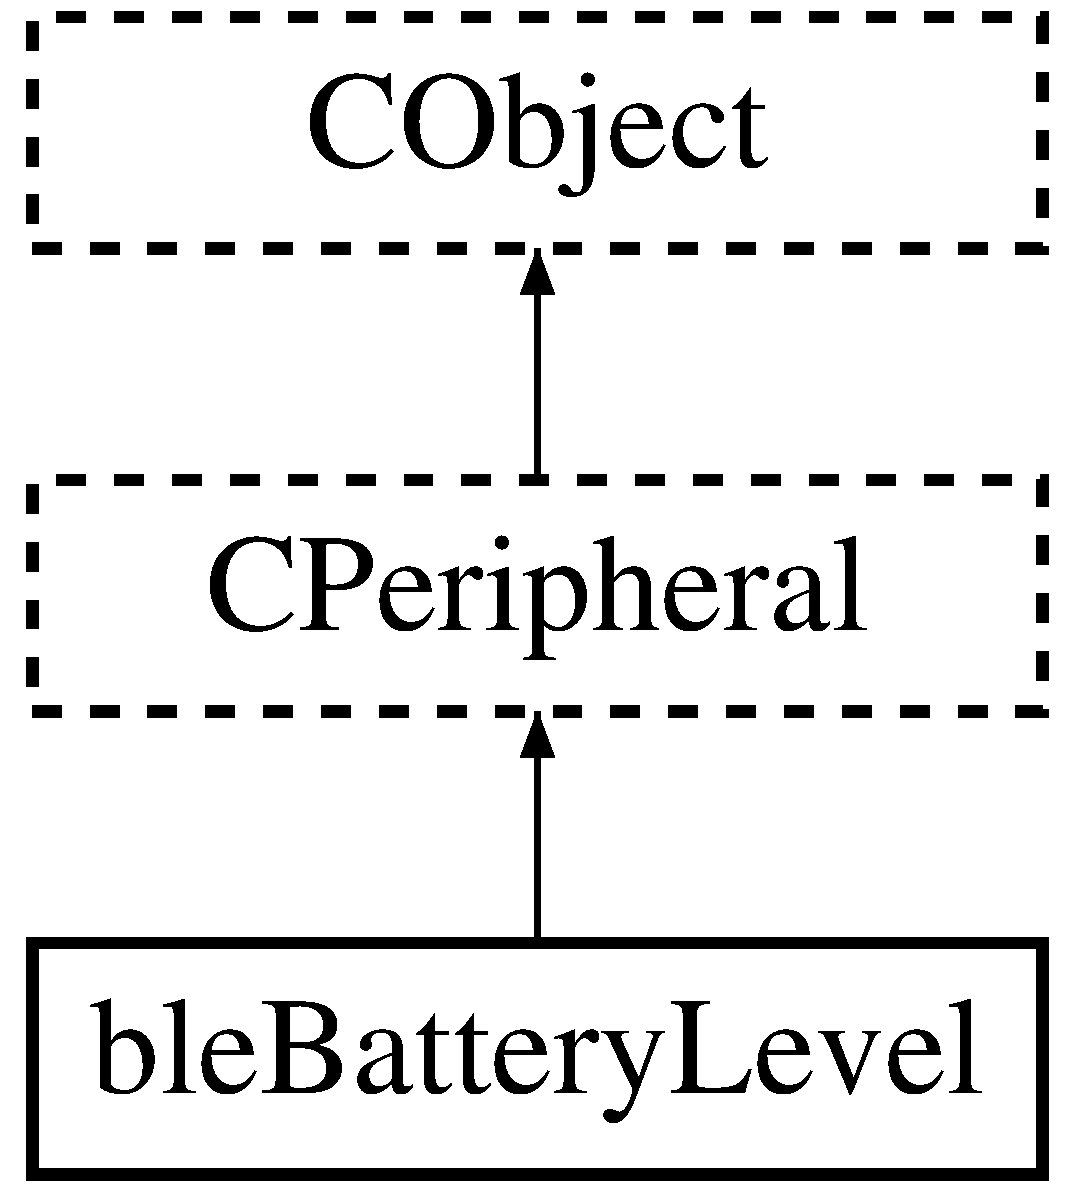
\includegraphics[height=3.000000cm]{d8/d3b/classble_battery_level}
\end{center}
\end{figure}
\subsection*{Public Member Functions}
\begin{DoxyCompactItemize}
\item 
\hyperlink{classble_battery_level_a212d349975b73b6f6020ce496ed68834}{ble\-Battery\-Level} (\hyperlink{classble_serial}{ble\-Serial} \&ble)
\item 
virtual bool \hyperlink{classble_battery_level_a2c6fae51a8653f720eb50169b094f7a5}{read\-System\-Voltage} (float \&voltage)
\item 
virtual bool \hyperlink{classble_battery_level_ad770083f87f2f193b897ca767593e716}{send\-Battery\-Level} (uint8\-\_\-t level)
\item 
virtual bool \hyperlink{classble_battery_level_a8cfd4674c5b405183b6b282e663849e4}{is\-Available} ()
\end{DoxyCompactItemize}
\subsection*{Protected Attributes}
\begin{DoxyCompactItemize}
\item 
\hyperlink{classble_serial}{ble\-Serial} $\ast$ \hyperlink{classble_battery_level_ac1466f5cc1995a2af27914beb432dedb}{m\-\_\-ble}
\end{DoxyCompactItemize}


\subsection{Detailed Description}
The \hyperlink{classble_battery_level}{ble\-Battery\-Level} class exposes the state of a battery within a device. 

\subsection{Constructor \& Destructor Documentation}
\hypertarget{classble_battery_level_a212d349975b73b6f6020ce496ed68834}{\index{ble\-Battery\-Level@{ble\-Battery\-Level}!ble\-Battery\-Level@{ble\-Battery\-Level}}
\index{ble\-Battery\-Level@{ble\-Battery\-Level}!bleBatteryLevel@{ble\-Battery\-Level}}
\subsubsection[{ble\-Battery\-Level}]{\setlength{\rightskip}{0pt plus 5cm}ble\-Battery\-Level\-::ble\-Battery\-Level (
\begin{DoxyParamCaption}
\item[{{\bf ble\-Serial} \&}]{ble}
\end{DoxyParamCaption}
)}}\label{classble_battery_level_a212d349975b73b6f6020ce496ed68834}
\hyperlink{classble_battery_level}{ble\-Battery\-Level} constructor. 
\begin{DoxyCode}
\textcolor{keywordtype}{int} main() \{
        ...
        \hyperlink{classble_serial}{bleSerial} ble(\textcolor{stringliteral}{"myBLE"});
        ble.enable();
        ...
        \hyperlink{classble_battery_level}{bleBatteryLevel} bat(ble);
        ...
        \textcolor{keywordtype}{float} val;
        uint8\_t level;

        \textcolor{keywordflow}{if} ( bat.readSystemVoltage(val) ) \{
         level = map(val, 2.0f, 3.3f, 0, 100);
         bat.sendBatteryLevel(level);
        \}
        ...
\end{DoxyCode}
 
\begin{DoxyParams}[1]{Parameters}
\mbox{\tt in}  & {\em ble} & is a \hyperlink{classble_serial}{ble\-Serial} class object. \\
\hline
\end{DoxyParams}


\subsection{Member Function Documentation}
\hypertarget{classble_battery_level_a2c6fae51a8653f720eb50169b094f7a5}{\index{ble\-Battery\-Level@{ble\-Battery\-Level}!read\-System\-Voltage@{read\-System\-Voltage}}
\index{read\-System\-Voltage@{read\-System\-Voltage}!bleBatteryLevel@{ble\-Battery\-Level}}
\subsubsection[{read\-System\-Voltage}]{\setlength{\rightskip}{0pt plus 5cm}virtual bool ble\-Battery\-Level\-::read\-System\-Voltage (
\begin{DoxyParamCaption}
\item[{float \&}]{voltage}
\end{DoxyParamCaption}
)\hspace{0.3cm}{\ttfamily [virtual]}}}\label{classble_battery_level_a2c6fae51a8653f720eb50169b094f7a5}
Use read\-System\-Voltage to retrieve the voltage of system (V3.\-3). 
\begin{DoxyParams}[1]{Parameters}
\mbox{\tt out}  & {\em voltage} & is a float type data to receive the system voltage. \\
\hline
\end{DoxyParams}
\begin{DoxyReturn}{Returns}
true, if read system voltage successful. otherwise, read failed. 
\end{DoxyReturn}
\hypertarget{classble_battery_level_ad770083f87f2f193b897ca767593e716}{\index{ble\-Battery\-Level@{ble\-Battery\-Level}!send\-Battery\-Level@{send\-Battery\-Level}}
\index{send\-Battery\-Level@{send\-Battery\-Level}!bleBatteryLevel@{ble\-Battery\-Level}}
\subsubsection[{send\-Battery\-Level}]{\setlength{\rightskip}{0pt plus 5cm}virtual bool ble\-Battery\-Level\-::send\-Battery\-Level (
\begin{DoxyParamCaption}
\item[{uint8\-\_\-t}]{level}
\end{DoxyParamCaption}
)\hspace{0.3cm}{\ttfamily [virtual]}}}\label{classble_battery_level_ad770083f87f2f193b897ca767593e716}
Use send\-Battery\-Level to send the battery level to remote (App). 
\begin{DoxyParams}[1]{Parameters}
\mbox{\tt in}  & {\em level} & is an unit8\-\_\-t type integer to indicate the battery level percentage. (0$\sim$100\%) \\
\hline
\end{DoxyParams}
\begin{DoxyReturn}{Returns}
true, if send battery level successful. otherwise, if send failed. 
\end{DoxyReturn}
\hypertarget{classble_battery_level_a8cfd4674c5b405183b6b282e663849e4}{\index{ble\-Battery\-Level@{ble\-Battery\-Level}!is\-Available@{is\-Available}}
\index{is\-Available@{is\-Available}!bleBatteryLevel@{ble\-Battery\-Level}}
\subsubsection[{is\-Available}]{\setlength{\rightskip}{0pt plus 5cm}virtual bool ble\-Battery\-Level\-::is\-Available (
\begin{DoxyParamCaption}
{}
\end{DoxyParamCaption}
)\hspace{0.3cm}{\ttfamily [virtual]}}}\label{classble_battery_level_a8cfd4674c5b405183b6b282e663849e4}
Use is\-Available to check the service whether opened by remote (App). \begin{DoxyReturn}{Returns}
true, if service is available. otherwise, the service is not in used. 
\end{DoxyReturn}


\subsection{Member Data Documentation}
\hypertarget{classble_battery_level_ac1466f5cc1995a2af27914beb432dedb}{\index{ble\-Battery\-Level@{ble\-Battery\-Level}!m\-\_\-ble@{m\-\_\-ble}}
\index{m\-\_\-ble@{m\-\_\-ble}!bleBatteryLevel@{ble\-Battery\-Level}}
\subsubsection[{m\-\_\-ble}]{\setlength{\rightskip}{0pt plus 5cm}{\bf ble\-Serial}$\ast$ ble\-Battery\-Level\-::m\-\_\-ble\hspace{0.3cm}{\ttfamily [protected]}}}\label{classble_battery_level_ac1466f5cc1995a2af27914beb432dedb}


The documentation for this class was generated from the following file\-:\begin{DoxyCompactItemize}
\item 
ble\-\_\-battery.\-h\end{DoxyCompactItemize}

\hypertarget{classble_device_info}{\section{ble\-Device\-Info Class Reference}
\label{classble_device_info}\index{ble\-Device\-Info@{ble\-Device\-Info}}
}


{\ttfamily \#include \char`\"{}class/ble\-\_\-devinfo.\-h\char`\"{}}

Inheritance diagram for ble\-Device\-Info\-:\begin{figure}[H]
\begin{center}
\leavevmode
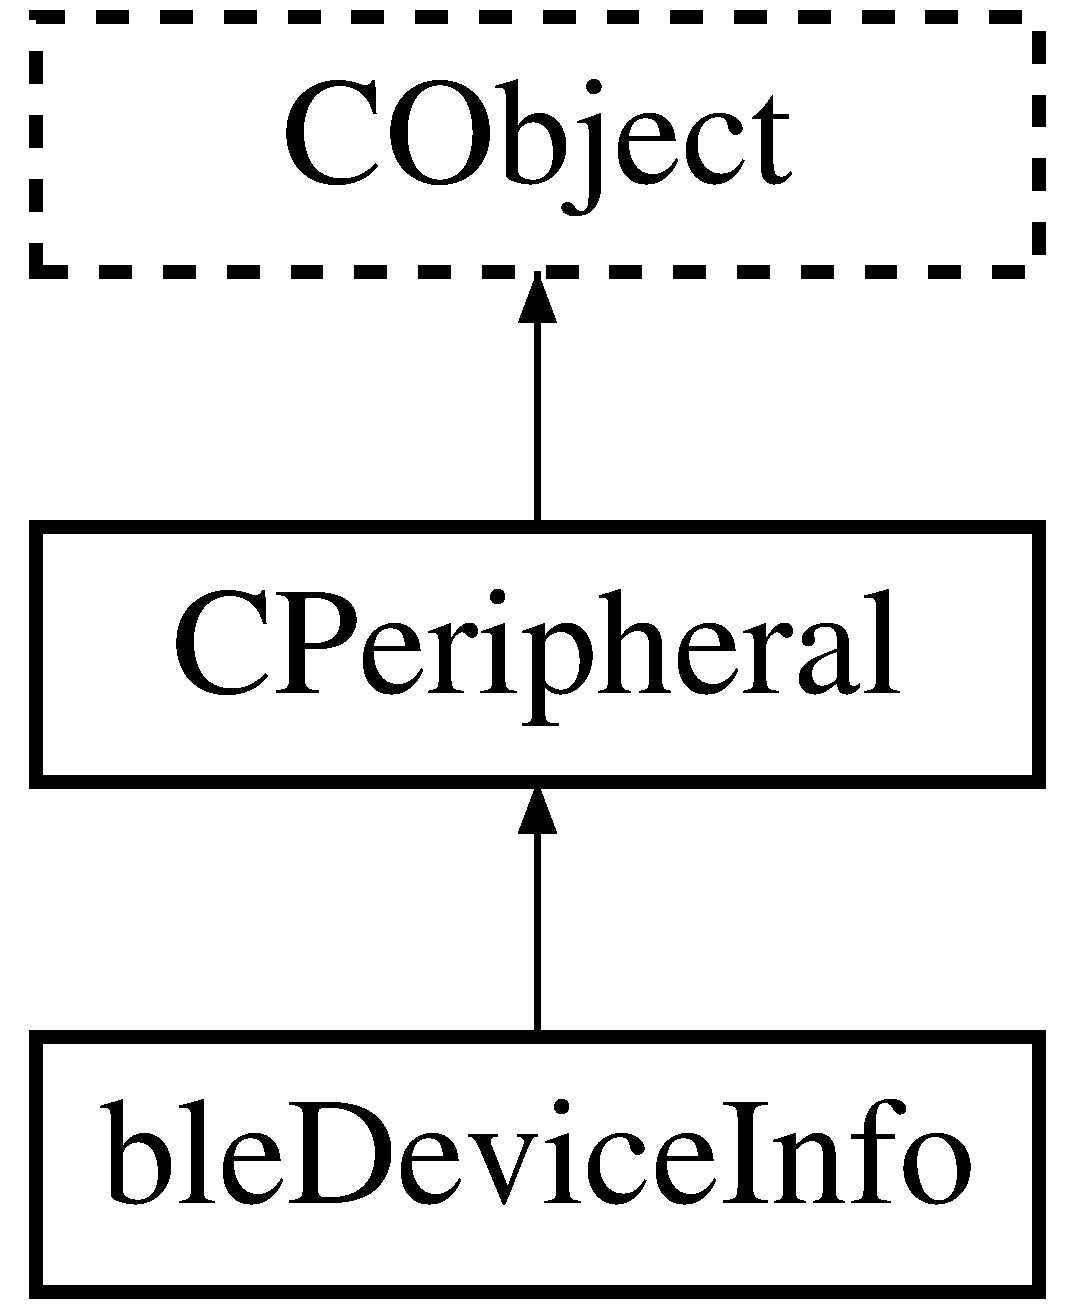
\includegraphics[height=3.000000cm]{d3/dc5/classble_device_info}
\end{center}
\end{figure}
\subsection*{Public Member Functions}
\begin{DoxyCompactItemize}
\item 
\hyperlink{classble_device_info_ae5f10713f4db98be9245aff3d482d51d}{ble\-Device\-Info} (\hyperlink{classble_serial}{ble\-Serial} \&ble)
\item 
int \hyperlink{classble_device_info_a98d7f5689f1e769f396282e3511edb99}{set\-Manufacture\-Name} (L\-P\-C\-T\-S\-T\-R str)
\item 
int \hyperlink{classble_device_info_a9e6a9696bb974ba0175968b3057e68d0}{set\-Model\-Number} (L\-P\-C\-T\-S\-T\-R str)
\item 
int \hyperlink{classble_device_info_a03fce5e655451a1245643987ca15ba71}{set\-Serial\-Number} (L\-P\-C\-T\-S\-T\-R str)
\item 
int \hyperlink{classble_device_info_a0e8825ee5d745fafdca6525fa2c230e7}{set\-Firmware\-Revison} (L\-P\-C\-T\-S\-T\-R str)
\item 
int \hyperlink{classble_device_info_aa2a08fe14dd55d02255719a1d29a484f}{set\-Hardware\-Revision} (L\-P\-C\-T\-S\-T\-R str)
\item 
void \hyperlink{classble_device_info_a372ab0246f7e19548fcef771e06dc407}{set\-System\-Id} (S\-Y\-S\-\_\-\-I\-D\-\_\-\-T \&sys\-Id)
\item 
void \hyperlink{classble_device_info_a344d50adf41337464686f926c8c85748}{set\-Pn\-P} (\hyperlink{group___enumerations_ga42b352f4817787f82d2adcffd4793ad9}{V\-I\-D\-\_\-\-S\-O\-U\-R\-C\-E\-\_\-\-T} src, uint16\-\_\-t vendor\-Id, uint16\-\_\-t product\-Id, uint16\-\_\-t product\-Version)
\end{DoxyCompactItemize}


\subsection{Detailed Description}
\hyperlink{classble_device_info}{ble\-Device\-Info} provides the Device Information service in B\-L\-E device. 

\subsection{Constructor \& Destructor Documentation}
\hypertarget{classble_device_info_ae5f10713f4db98be9245aff3d482d51d}{\index{ble\-Device\-Info@{ble\-Device\-Info}!ble\-Device\-Info@{ble\-Device\-Info}}
\index{ble\-Device\-Info@{ble\-Device\-Info}!bleDeviceInfo@{ble\-Device\-Info}}
\subsubsection[{ble\-Device\-Info}]{\setlength{\rightskip}{0pt plus 5cm}ble\-Device\-Info\-::ble\-Device\-Info (
\begin{DoxyParamCaption}
\item[{{\bf ble\-Serial} \&}]{ble}
\end{DoxyParamCaption}
)}}\label{classble_device_info_ae5f10713f4db98be9245aff3d482d51d}


\subsection{Member Function Documentation}
\hypertarget{classble_device_info_a98d7f5689f1e769f396282e3511edb99}{\index{ble\-Device\-Info@{ble\-Device\-Info}!set\-Manufacture\-Name@{set\-Manufacture\-Name}}
\index{set\-Manufacture\-Name@{set\-Manufacture\-Name}!bleDeviceInfo@{ble\-Device\-Info}}
\subsubsection[{set\-Manufacture\-Name}]{\setlength{\rightskip}{0pt plus 5cm}int ble\-Device\-Info\-::set\-Manufacture\-Name (
\begin{DoxyParamCaption}
\item[{L\-P\-C\-T\-S\-T\-R}]{str}
\end{DoxyParamCaption}
)}}\label{classble_device_info_a98d7f5689f1e769f396282e3511edb99}
\hypertarget{classble_device_info_a9e6a9696bb974ba0175968b3057e68d0}{\index{ble\-Device\-Info@{ble\-Device\-Info}!set\-Model\-Number@{set\-Model\-Number}}
\index{set\-Model\-Number@{set\-Model\-Number}!bleDeviceInfo@{ble\-Device\-Info}}
\subsubsection[{set\-Model\-Number}]{\setlength{\rightskip}{0pt plus 5cm}int ble\-Device\-Info\-::set\-Model\-Number (
\begin{DoxyParamCaption}
\item[{L\-P\-C\-T\-S\-T\-R}]{str}
\end{DoxyParamCaption}
)}}\label{classble_device_info_a9e6a9696bb974ba0175968b3057e68d0}
\hypertarget{classble_device_info_a03fce5e655451a1245643987ca15ba71}{\index{ble\-Device\-Info@{ble\-Device\-Info}!set\-Serial\-Number@{set\-Serial\-Number}}
\index{set\-Serial\-Number@{set\-Serial\-Number}!bleDeviceInfo@{ble\-Device\-Info}}
\subsubsection[{set\-Serial\-Number}]{\setlength{\rightskip}{0pt plus 5cm}int ble\-Device\-Info\-::set\-Serial\-Number (
\begin{DoxyParamCaption}
\item[{L\-P\-C\-T\-S\-T\-R}]{str}
\end{DoxyParamCaption}
)}}\label{classble_device_info_a03fce5e655451a1245643987ca15ba71}
\hypertarget{classble_device_info_a0e8825ee5d745fafdca6525fa2c230e7}{\index{ble\-Device\-Info@{ble\-Device\-Info}!set\-Firmware\-Revison@{set\-Firmware\-Revison}}
\index{set\-Firmware\-Revison@{set\-Firmware\-Revison}!bleDeviceInfo@{ble\-Device\-Info}}
\subsubsection[{set\-Firmware\-Revison}]{\setlength{\rightskip}{0pt plus 5cm}int ble\-Device\-Info\-::set\-Firmware\-Revison (
\begin{DoxyParamCaption}
\item[{L\-P\-C\-T\-S\-T\-R}]{str}
\end{DoxyParamCaption}
)}}\label{classble_device_info_a0e8825ee5d745fafdca6525fa2c230e7}
\hypertarget{classble_device_info_aa2a08fe14dd55d02255719a1d29a484f}{\index{ble\-Device\-Info@{ble\-Device\-Info}!set\-Hardware\-Revision@{set\-Hardware\-Revision}}
\index{set\-Hardware\-Revision@{set\-Hardware\-Revision}!bleDeviceInfo@{ble\-Device\-Info}}
\subsubsection[{set\-Hardware\-Revision}]{\setlength{\rightskip}{0pt plus 5cm}int ble\-Device\-Info\-::set\-Hardware\-Revision (
\begin{DoxyParamCaption}
\item[{L\-P\-C\-T\-S\-T\-R}]{str}
\end{DoxyParamCaption}
)}}\label{classble_device_info_aa2a08fe14dd55d02255719a1d29a484f}
\hypertarget{classble_device_info_a372ab0246f7e19548fcef771e06dc407}{\index{ble\-Device\-Info@{ble\-Device\-Info}!set\-System\-Id@{set\-System\-Id}}
\index{set\-System\-Id@{set\-System\-Id}!bleDeviceInfo@{ble\-Device\-Info}}
\subsubsection[{set\-System\-Id}]{\setlength{\rightskip}{0pt plus 5cm}void ble\-Device\-Info\-::set\-System\-Id (
\begin{DoxyParamCaption}
\item[{S\-Y\-S\-\_\-\-I\-D\-\_\-\-T \&}]{sys\-Id}
\end{DoxyParamCaption}
)}}\label{classble_device_info_a372ab0246f7e19548fcef771e06dc407}
\hypertarget{classble_device_info_a344d50adf41337464686f926c8c85748}{\index{ble\-Device\-Info@{ble\-Device\-Info}!set\-Pn\-P@{set\-Pn\-P}}
\index{set\-Pn\-P@{set\-Pn\-P}!bleDeviceInfo@{ble\-Device\-Info}}
\subsubsection[{set\-Pn\-P}]{\setlength{\rightskip}{0pt plus 5cm}void ble\-Device\-Info\-::set\-Pn\-P (
\begin{DoxyParamCaption}
\item[{{\bf V\-I\-D\-\_\-\-S\-O\-U\-R\-C\-E\-\_\-\-T}}]{src, }
\item[{uint16\-\_\-t}]{vendor\-Id, }
\item[{uint16\-\_\-t}]{product\-Id, }
\item[{uint16\-\_\-t}]{product\-Version}
\end{DoxyParamCaption}
)}}\label{classble_device_info_a344d50adf41337464686f926c8c85748}


The documentation for this class was generated from the following file\-:\begin{DoxyCompactItemize}
\item 
ble\-\_\-devinfo.\-h\end{DoxyCompactItemize}

\hypertarget{classble_health_thermometer}{\section{ble\-Health\-Thermometer Class Reference}
\label{classble_health_thermometer}\index{ble\-Health\-Thermometer@{ble\-Health\-Thermometer}}
}


{\ttfamily \#include \char`\"{}class/ble\-\_\-ht.\-h\char`\"{}}

Inheritance diagram for ble\-Health\-Thermometer\-:\begin{figure}[H]
\begin{center}
\leavevmode
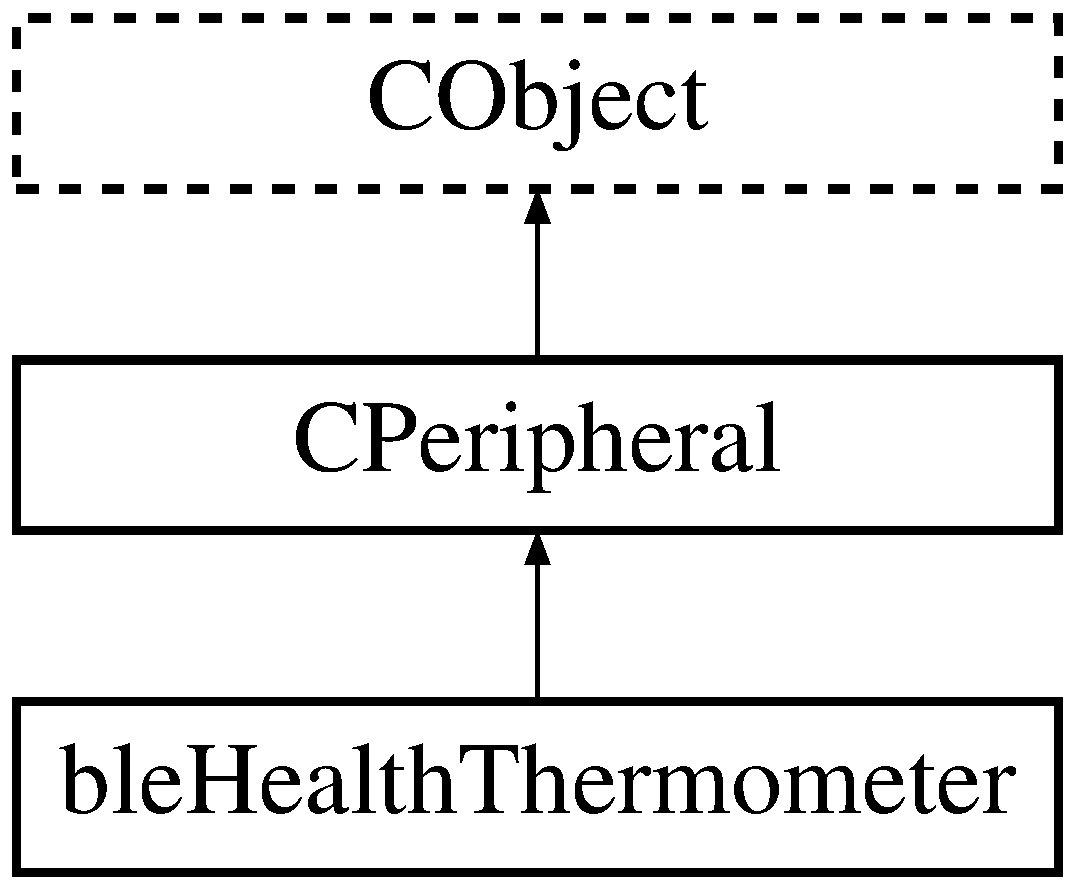
\includegraphics[height=3.000000cm]{d9/d26/classble_health_thermometer}
\end{center}
\end{figure}
\subsection*{Public Member Functions}
\begin{DoxyCompactItemize}
\item 
\hyperlink{classble_health_thermometer_a92480888b6ed2b0fe354cc4a5404a63d}{ble\-Health\-Thermometer} (\hyperlink{classble_serial}{ble\-Serial} \&ble, \hyperlink{group___enumerations_ga7fa712ec2096ff24507538b50e2f51e0}{h\-\_\-temp\-\_\-type\-\_\-t} type=\hyperlink{group___enumerations_gga7fa712ec2096ff24507538b50e2f51e0aedd58ca967667d8b42f7eef6080719e0}{H\-\_\-\-T\-Y\-P\-E\-\_\-\-N\-O\-T\-\_\-\-I\-N\-C\-L\-U\-D\-E\-D})
\item 
void \hyperlink{classble_health_thermometer_a0f00efd291e5b91fef286071d3441172}{unit\-\_\-c} ()
\item 
void \hyperlink{classble_health_thermometer_aafe2468db4033c905394da1d58c83620}{unit\-\_\-f} ()
\item 
virtual void \hyperlink{classble_health_thermometer_acd9cde127f632f06615382b3d03299fd}{measurement\-Interval} (uint16\-\_\-t sec)
\item 
virtual bool \hyperlink{classble_health_thermometer_a09413d493022f3c52dfd269cf01bacd1}{send\-Measure} (float temp)
\item 
virtual void \hyperlink{classble_health_thermometer_a32d3cdc9efb78bed4a5ed728cdb93846}{set\-Dynamic\-Type} (\hyperlink{group___enumerations_ga7fa712ec2096ff24507538b50e2f51e0}{h\-\_\-temp\-\_\-type\-\_\-t} in\-\_\-type)
\item 
virtual bool \hyperlink{classble_health_thermometer_a39b5e5ae997a87c7393e363cb540c421}{is\-Available} ()
\item 
bool \hyperlink{classble_health_thermometer_a8d54f2c7e49f12ca5846e55dcab0ab3b}{read\-Temperature} (float \&temp)
\end{DoxyCompactItemize}


\subsection{Detailed Description}
The \hyperlink{classble_health_thermometer}{ble\-Health\-Thermometer} class exposes temperature and other data from a thermometer intended for healthcare and fitness applications. 

\subsection{Constructor \& Destructor Documentation}
\hypertarget{classble_health_thermometer_a92480888b6ed2b0fe354cc4a5404a63d}{\index{ble\-Health\-Thermometer@{ble\-Health\-Thermometer}!ble\-Health\-Thermometer@{ble\-Health\-Thermometer}}
\index{ble\-Health\-Thermometer@{ble\-Health\-Thermometer}!bleHealthThermometer@{ble\-Health\-Thermometer}}
\subsubsection[{ble\-Health\-Thermometer}]{\setlength{\rightskip}{0pt plus 5cm}ble\-Health\-Thermometer\-::ble\-Health\-Thermometer (
\begin{DoxyParamCaption}
\item[{{\bf ble\-Serial} \&}]{ble, }
\item[{{\bf h\-\_\-temp\-\_\-type\-\_\-t}}]{type = {\ttfamily {\bf H\-\_\-\-T\-Y\-P\-E\-\_\-\-N\-O\-T\-\_\-\-I\-N\-C\-L\-U\-D\-E\-D}}}
\end{DoxyParamCaption}
)}}\label{classble_health_thermometer_a92480888b6ed2b0fe354cc4a5404a63d}
\hyperlink{classble_health_thermometer}{ble\-Health\-Thermometer} constructor. 
\begin{DoxyCode}
\textcolor{keywordtype}{int} main() \{
    ...
    \hyperlink{classble_serial}{bleSerial} ble(\textcolor{stringliteral}{"myBLE"});
    ble.enable();
    ...
    \hyperlink{classble_health_thermometer}{bleHealthThermometer} ht(ble);
    ht.unit\_c();
    ht.measurementInterval(3);  \textcolor{comment}{// set measurement interval 3 seconds}
    ...
    ht.sendMeasure(temp);
    ...
\end{DoxyCode}
 
\begin{DoxyParams}[1]{Parameters}
\mbox{\tt in}  & {\em ble} & is a \hyperlink{classble_serial}{ble\-Serial} class object. \\
\hline
\mbox{\tt in}  & {\em type} & is a h\-\_\-temp\-\_\-type\-\_\-t enumeration. \\
\hline
\end{DoxyParams}


\subsection{Member Function Documentation}
\hypertarget{classble_health_thermometer_a0f00efd291e5b91fef286071d3441172}{\index{ble\-Health\-Thermometer@{ble\-Health\-Thermometer}!unit\-\_\-c@{unit\-\_\-c}}
\index{unit\-\_\-c@{unit\-\_\-c}!bleHealthThermometer@{ble\-Health\-Thermometer}}
\subsubsection[{unit\-\_\-c}]{\setlength{\rightskip}{0pt plus 5cm}void ble\-Health\-Thermometer\-::unit\-\_\-c (
\begin{DoxyParamCaption}
{}
\end{DoxyParamCaption}
)}}\label{classble_health_thermometer_a0f00efd291e5b91fef286071d3441172}
Set temperature unit to Celsius. \hypertarget{classble_health_thermometer_aafe2468db4033c905394da1d58c83620}{\index{ble\-Health\-Thermometer@{ble\-Health\-Thermometer}!unit\-\_\-f@{unit\-\_\-f}}
\index{unit\-\_\-f@{unit\-\_\-f}!bleHealthThermometer@{ble\-Health\-Thermometer}}
\subsubsection[{unit\-\_\-f}]{\setlength{\rightskip}{0pt plus 5cm}void ble\-Health\-Thermometer\-::unit\-\_\-f (
\begin{DoxyParamCaption}
{}
\end{DoxyParamCaption}
)}}\label{classble_health_thermometer_aafe2468db4033c905394da1d58c83620}
Set temperature unit to Fahrenheit. \hypertarget{classble_health_thermometer_acd9cde127f632f06615382b3d03299fd}{\index{ble\-Health\-Thermometer@{ble\-Health\-Thermometer}!measurement\-Interval@{measurement\-Interval}}
\index{measurement\-Interval@{measurement\-Interval}!bleHealthThermometer@{ble\-Health\-Thermometer}}
\subsubsection[{measurement\-Interval}]{\setlength{\rightskip}{0pt plus 5cm}virtual void ble\-Health\-Thermometer\-::measurement\-Interval (
\begin{DoxyParamCaption}
\item[{uint16\-\_\-t}]{sec}
\end{DoxyParamCaption}
)\hspace{0.3cm}{\ttfamily [virtual]}}}\label{classble_health_thermometer_acd9cde127f632f06615382b3d03299fd}
Set measurement interval (unit second, default 3 seconds) 
\begin{DoxyParams}{Parameters}
{\em sec} & is an uint16\-\_\-t integer to indicate the measurement interval. \\
\hline
\end{DoxyParams}
\hypertarget{classble_health_thermometer_a09413d493022f3c52dfd269cf01bacd1}{\index{ble\-Health\-Thermometer@{ble\-Health\-Thermometer}!send\-Measure@{send\-Measure}}
\index{send\-Measure@{send\-Measure}!bleHealthThermometer@{ble\-Health\-Thermometer}}
\subsubsection[{send\-Measure}]{\setlength{\rightskip}{0pt plus 5cm}virtual bool ble\-Health\-Thermometer\-::send\-Measure (
\begin{DoxyParamCaption}
\item[{float}]{temp}
\end{DoxyParamCaption}
)\hspace{0.3cm}{\ttfamily [virtual]}}}\label{classble_health_thermometer_a09413d493022f3c52dfd269cf01bacd1}
send temperature measurement 
\begin{DoxyParams}{Parameters}
{\em temp} & is a floating value to indicate the temperature. \\
\hline
\end{DoxyParams}
\begin{DoxyReturn}{Returns}
true, if send measure successful. otherwise, send failed. 
\end{DoxyReturn}
\hypertarget{classble_health_thermometer_a32d3cdc9efb78bed4a5ed728cdb93846}{\index{ble\-Health\-Thermometer@{ble\-Health\-Thermometer}!set\-Dynamic\-Type@{set\-Dynamic\-Type}}
\index{set\-Dynamic\-Type@{set\-Dynamic\-Type}!bleHealthThermometer@{ble\-Health\-Thermometer}}
\subsubsection[{set\-Dynamic\-Type}]{\setlength{\rightskip}{0pt plus 5cm}virtual void ble\-Health\-Thermometer\-::set\-Dynamic\-Type (
\begin{DoxyParamCaption}
\item[{{\bf h\-\_\-temp\-\_\-type\-\_\-t}}]{in\-\_\-type}
\end{DoxyParamCaption}
)\hspace{0.3cm}{\ttfamily [virtual]}}}\label{classble_health_thermometer_a32d3cdc9efb78bed4a5ed728cdb93846}
Set the temperature dynamic type 
\begin{DoxyParams}[1]{Parameters}
\mbox{\tt in}  & {\em in\-\_\-type} & is a h\-\_\-temp\-\_\-type enumeration. \\
\hline
\end{DoxyParams}
\hypertarget{classble_health_thermometer_a39b5e5ae997a87c7393e363cb540c421}{\index{ble\-Health\-Thermometer@{ble\-Health\-Thermometer}!is\-Available@{is\-Available}}
\index{is\-Available@{is\-Available}!bleHealthThermometer@{ble\-Health\-Thermometer}}
\subsubsection[{is\-Available}]{\setlength{\rightskip}{0pt plus 5cm}virtual bool ble\-Health\-Thermometer\-::is\-Available (
\begin{DoxyParamCaption}
{}
\end{DoxyParamCaption}
)\hspace{0.3cm}{\ttfamily [virtual]}}}\label{classble_health_thermometer_a39b5e5ae997a87c7393e363cb540c421}
Use is\-Available to check the service whether opened by remote (App). \begin{DoxyReturn}{Returns}
true, if service is available. otherwise, the service is not in used. 
\end{DoxyReturn}
\hypertarget{classble_health_thermometer_a8d54f2c7e49f12ca5846e55dcab0ab3b}{\index{ble\-Health\-Thermometer@{ble\-Health\-Thermometer}!read\-Temperature@{read\-Temperature}}
\index{read\-Temperature@{read\-Temperature}!bleHealthThermometer@{ble\-Health\-Thermometer}}
\subsubsection[{read\-Temperature}]{\setlength{\rightskip}{0pt plus 5cm}bool ble\-Health\-Thermometer\-::read\-Temperature (
\begin{DoxyParamCaption}
\item[{float \&}]{temp}
\end{DoxyParamCaption}
)}}\label{classble_health_thermometer_a8d54f2c7e49f12ca5846e55dcab0ab3b}
Use read\-Temperature to read the temperature from B\-L\-E core sensor 
\begin{DoxyParams}[1]{Parameters}
\mbox{\tt out}  & {\em temp} & is a floating value to receive the temperature. \\
\hline
\end{DoxyParams}
\begin{DoxyReturn}{Returns}
true, if read temperature successful. otherwise, read failed. 
\end{DoxyReturn}


The documentation for this class was generated from the following file\-:\begin{DoxyCompactItemize}
\item 
ble\-\_\-ht.\-h\end{DoxyCompactItemize}

\hypertarget{classble_heart_rate}{\section{ble\-Heart\-Rate Class Reference}
\label{classble_heart_rate}\index{ble\-Heart\-Rate@{ble\-Heart\-Rate}}
}


{\ttfamily \#include $<$ble\-\_\-heartrate.\-h$>$}

Inheritance diagram for ble\-Heart\-Rate\-:\begin{figure}[H]
\begin{center}
\leavevmode
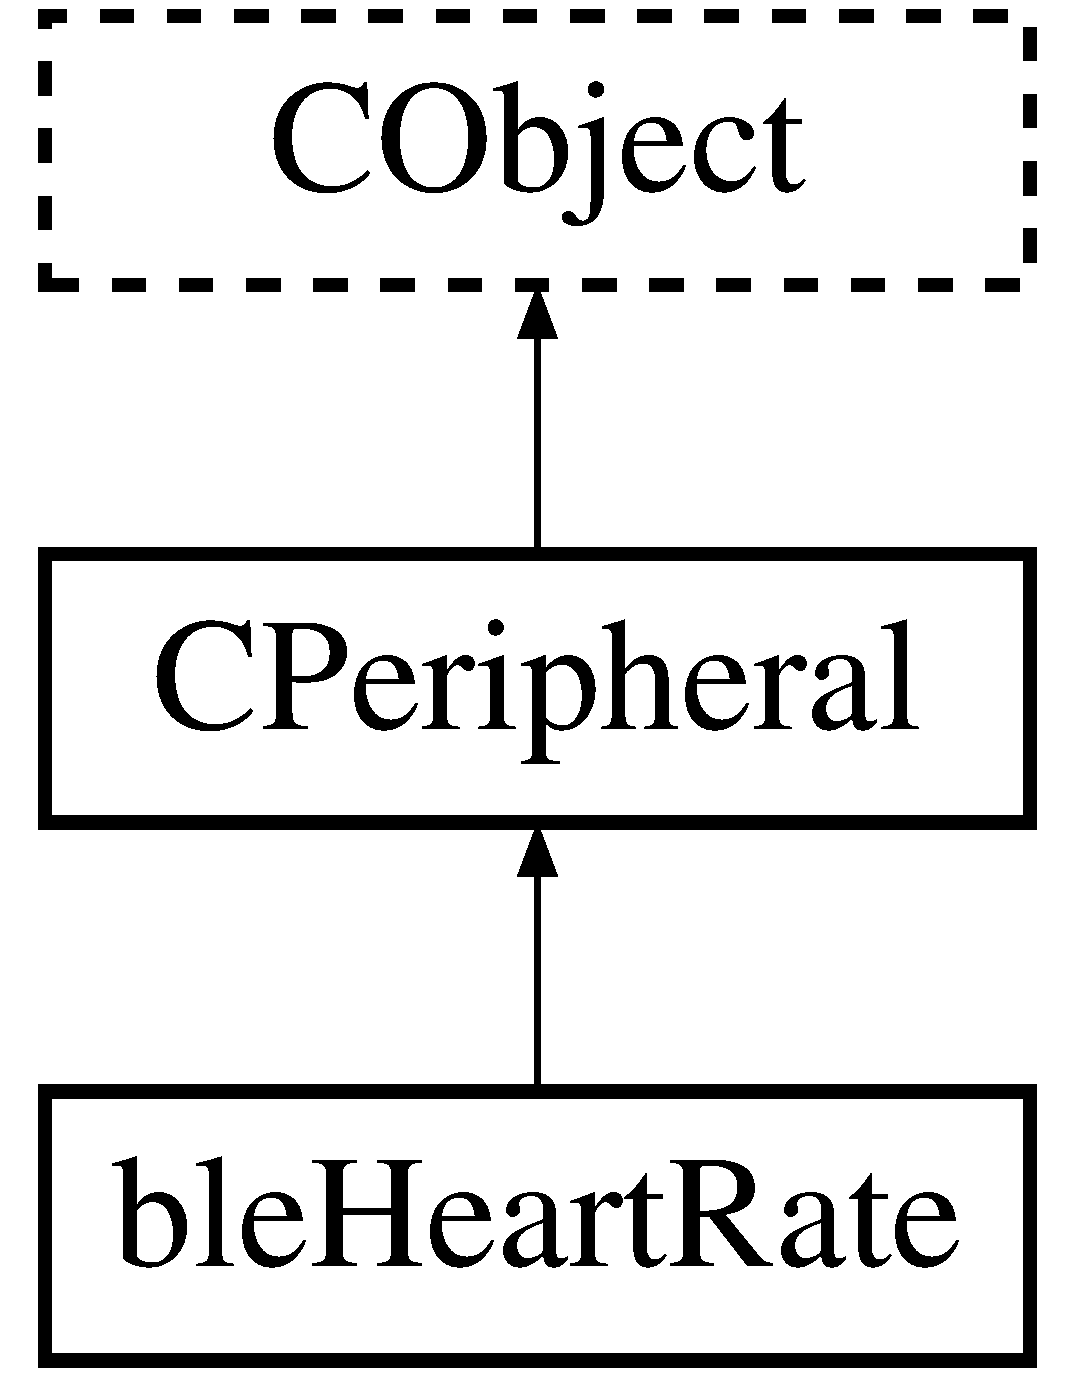
\includegraphics[height=3.000000cm]{d3/d81/classble_heart_rate}
\end{center}
\end{figure}
\subsection*{Public Member Functions}
\begin{DoxyCompactItemize}
\item 
\hyperlink{classble_heart_rate_af5e0bc81b5d2f8e290b6cba8050f80c2}{ble\-Heart\-Rate} (\hyperlink{classble_serial}{ble\-Serial} \&ble)
\item 
virtual bool \hyperlink{classble_heart_rate_a822019806bf50f6d25ae075b62a838ab}{is\-Available} ()
\item 
void \hyperlink{classble_heart_rate_acd5a0148a2df6692893a274a18710431}{support\-Contact} (bool enable)
\item 
void \hyperlink{classble_heart_rate_a4b05ceb33ffe7fcfe9f1a3dbf9679882}{contact\-Status} (bool enable)
\item 
void \hyperlink{classble_heart_rate_a9c822ea4fafcb609e009427feb0949c2}{set\-Sensor\-Location} (hrsl\-\_\-code\-\_\-t code)
\item 
bool \hyperlink{classble_heart_rate_a2b7329b1756f03c99334b6575e14c090}{send\-Measure} (uint8\-\_\-t meas\-\_\-hr)
\begin{DoxyCompactList}\small\item\em Overload function to send a heart rate measurement (8 bits). \end{DoxyCompactList}\item 
bool \hyperlink{classble_heart_rate_a9f69ad22553dabc5b992bf9a15aa6667}{send\-Measure} (uint16\-\_\-t meas\-\_\-hr)
\begin{DoxyCompactList}\small\item\em Function to send a heart rate measurement (16 bits). \end{DoxyCompactList}\item 
bool \hyperlink{classble_heart_rate_ac0bd83937f2997c2451918a421c277c2}{send\-Measure} (uint8\-\_\-t meas\-\_\-hr, uint16\-\_\-t expended\-\_\-energy)
\begin{DoxyCompactList}\small\item\em Overload function to send a heart rate measurement (8 bits) with expended energy. \end{DoxyCompactList}\item 
bool \hyperlink{classble_heart_rate_a34a055d4b926b2447ca78a4f63691d30}{send\-Measure} (uint16\-\_\-t meas\-\_\-hr, uint16\-\_\-t expended\-\_\-energy)
\begin{DoxyCompactList}\small\item\em Overload function to send a heart rate measurement (16 bits) with expended energy. \end{DoxyCompactList}\item 
bool \hyperlink{classble_heart_rate_ab511f6fcb6b7b57c09132911b5f87cb7}{send\-Measure} (uint8\-\_\-t meas\-\_\-hr, uint16\-\_\-t $\ast$p\-\_\-rr\-\_\-intervals, uint8\-\_\-t nb\-\_\-intervals)
\begin{DoxyCompactList}\small\item\em Overload function to send a heart rate measurement (8 bits) with rr\-\_\-intervals. \end{DoxyCompactList}\item 
bool \hyperlink{classble_heart_rate_a1d3fd3348703d304cd445620e7bb4998}{send\-Measure} (uint16\-\_\-t meas\-\_\-hr, uint16\-\_\-t $\ast$p\-\_\-rr\-\_\-intervals, uint8\-\_\-t nb\-\_\-intervals)
\begin{DoxyCompactList}\small\item\em Overload function to send a heart rate measurement (16 bits) with rr\-\_\-intervals. \end{DoxyCompactList}\item 
bool \hyperlink{classble_heart_rate_a2a6d1f10ea9a92ad5a953fc683125c50}{send\-Measure} (uint8\-\_\-t meas\-\_\-hr, uint16\-\_\-t expended\-\_\-energy, uint16\-\_\-t $\ast$p\-\_\-rr\-\_\-intervals, uint8\-\_\-t nb\-\_\-intervals)
\begin{DoxyCompactList}\small\item\em Overload function to send a heart rate measurement (8 bits) with expended energy with rr\-\_\-intervals. \end{DoxyCompactList}\item 
bool \hyperlink{classble_heart_rate_ab5cf3fd6c2e5909af4d51150c865d8b0}{send\-Measure} (uint16\-\_\-t meas\-\_\-hr, uint16\-\_\-t expended\-\_\-energy, uint16\-\_\-t $\ast$p\-\_\-rr\-\_\-intervals, uint8\-\_\-t nb\-\_\-intervals)
\begin{DoxyCompactList}\small\item\em Overload function to send a heart rate measurement (16 bits) with expended energy with rr\-\_\-intervals. \end{DoxyCompactList}\item 
virtual void \hyperlink{classble_heart_rate_a4764687c0e158518141b3dba9103b5d2}{on\-Reset\-Energy\-Expended} ()
\end{DoxyCompactItemize}


\subsection{Detailed Description}
The ble\-Hear\-Rate class exposes heart rate and other data from a Heart Rate Sensor intended for fitness applications. 

\subsection{Constructor \& Destructor Documentation}
\hypertarget{classble_heart_rate_af5e0bc81b5d2f8e290b6cba8050f80c2}{\index{ble\-Heart\-Rate@{ble\-Heart\-Rate}!ble\-Heart\-Rate@{ble\-Heart\-Rate}}
\index{ble\-Heart\-Rate@{ble\-Heart\-Rate}!bleHeartRate@{ble\-Heart\-Rate}}
\subsubsection[{ble\-Heart\-Rate}]{\setlength{\rightskip}{0pt plus 5cm}ble\-Heart\-Rate\-::ble\-Heart\-Rate (
\begin{DoxyParamCaption}
\item[{{\bf ble\-Serial} \&}]{ble}
\end{DoxyParamCaption}
)}}\label{classble_heart_rate_af5e0bc81b5d2f8e290b6cba8050f80c2}
\hyperlink{classble_heart_rate}{ble\-Heart\-Rate} constructor 
\begin{DoxyCode}
\textcolor{keywordtype}{int} main() \{
...
    \hyperlink{classble_serial}{bleSerial} ble(\textcolor{stringliteral}{"myBLE"});
    ble.enable();

    \hyperlink{classble_heart_rate}{bleHeartRate} hr(ble);
    hr.sendMeasure(BPM);
 ...
\end{DoxyCode}
 
\begin{DoxyParams}{Parameters}
{\em ble} & is a \hyperlink{classble_serial}{ble\-Serial} class object. \\
\hline
\end{DoxyParams}


\subsection{Member Function Documentation}
\hypertarget{classble_heart_rate_a822019806bf50f6d25ae075b62a838ab}{\index{ble\-Heart\-Rate@{ble\-Heart\-Rate}!is\-Available@{is\-Available}}
\index{is\-Available@{is\-Available}!bleHeartRate@{ble\-Heart\-Rate}}
\subsubsection[{is\-Available}]{\setlength{\rightskip}{0pt plus 5cm}virtual bool ble\-Heart\-Rate\-::is\-Available (
\begin{DoxyParamCaption}
{}
\end{DoxyParamCaption}
)\hspace{0.3cm}{\ttfamily [virtual]}}}\label{classble_heart_rate_a822019806bf50f6d25ae075b62a838ab}
Use is\-Available to check the service whether opened by remote (App). \begin{DoxyReturn}{Returns}
true, if service is available. otherwise, the service is not in used. 
\end{DoxyReturn}
\hypertarget{classble_heart_rate_acd5a0148a2df6692893a274a18710431}{\index{ble\-Heart\-Rate@{ble\-Heart\-Rate}!support\-Contact@{support\-Contact}}
\index{support\-Contact@{support\-Contact}!bleHeartRate@{ble\-Heart\-Rate}}
\subsubsection[{support\-Contact}]{\setlength{\rightskip}{0pt plus 5cm}void ble\-Heart\-Rate\-::support\-Contact (
\begin{DoxyParamCaption}
\item[{bool}]{enable}
\end{DoxyParamCaption}
)}}\label{classble_heart_rate_acd5a0148a2df6692893a274a18710431}
Set supported Contact sensor feature 
\begin{DoxyParams}{Parameters}
{\em enable} & true, if support the contact sensor. otherwise, no contact sensor supported. \\
\hline
\end{DoxyParams}
\hypertarget{classble_heart_rate_a4b05ceb33ffe7fcfe9f1a3dbf9679882}{\index{ble\-Heart\-Rate@{ble\-Heart\-Rate}!contact\-Status@{contact\-Status}}
\index{contact\-Status@{contact\-Status}!bleHeartRate@{ble\-Heart\-Rate}}
\subsubsection[{contact\-Status}]{\setlength{\rightskip}{0pt plus 5cm}void ble\-Heart\-Rate\-::contact\-Status (
\begin{DoxyParamCaption}
\item[{bool}]{enable}
\end{DoxyParamCaption}
)}}\label{classble_heart_rate_a4b05ceb33ffe7fcfe9f1a3dbf9679882}
Set contact sensor status. 
\begin{DoxyParams}{Parameters}
{\em enable} & is a boolean value, set true, if contact is detected. otherwise, contact is not detected. \\
\hline
\end{DoxyParams}
\hypertarget{classble_heart_rate_a9c822ea4fafcb609e009427feb0949c2}{\index{ble\-Heart\-Rate@{ble\-Heart\-Rate}!set\-Sensor\-Location@{set\-Sensor\-Location}}
\index{set\-Sensor\-Location@{set\-Sensor\-Location}!bleHeartRate@{ble\-Heart\-Rate}}
\subsubsection[{set\-Sensor\-Location}]{\setlength{\rightskip}{0pt plus 5cm}void ble\-Heart\-Rate\-::set\-Sensor\-Location (
\begin{DoxyParamCaption}
\item[{hrsl\-\_\-code\-\_\-t}]{code}
\end{DoxyParamCaption}
)}}\label{classble_heart_rate_a9c822ea4fafcb609e009427feb0949c2}
Set sensor location. 
\begin{DoxyParams}{Parameters}
{\em code} & is a hrsl\-\_\-code\-\_\-t enumeration. \\
\hline
\end{DoxyParams}
\hypertarget{classble_heart_rate_a2b7329b1756f03c99334b6575e14c090}{\index{ble\-Heart\-Rate@{ble\-Heart\-Rate}!send\-Measure@{send\-Measure}}
\index{send\-Measure@{send\-Measure}!bleHeartRate@{ble\-Heart\-Rate}}
\subsubsection[{send\-Measure}]{\setlength{\rightskip}{0pt plus 5cm}bool ble\-Heart\-Rate\-::send\-Measure (
\begin{DoxyParamCaption}
\item[{uint8\-\_\-t}]{meas\-\_\-hr}
\end{DoxyParamCaption}
)}}\label{classble_heart_rate_a2b7329b1756f03c99334b6575e14c090}


Overload function to send a heart rate measurement (8 bits). 


\begin{DoxyParams}{Parameters}
{\em meas\-\_\-hr} & Measured heart\-\_\-rate to send. \\
\hline
\end{DoxyParams}
\begin{DoxyReturn}{Returns}
\-: True when the command send successfully. 
\end{DoxyReturn}
\hypertarget{classble_heart_rate_a9f69ad22553dabc5b992bf9a15aa6667}{\index{ble\-Heart\-Rate@{ble\-Heart\-Rate}!send\-Measure@{send\-Measure}}
\index{send\-Measure@{send\-Measure}!bleHeartRate@{ble\-Heart\-Rate}}
\subsubsection[{send\-Measure}]{\setlength{\rightskip}{0pt plus 5cm}bool ble\-Heart\-Rate\-::send\-Measure (
\begin{DoxyParamCaption}
\item[{uint16\-\_\-t}]{meas\-\_\-hr}
\end{DoxyParamCaption}
)}}\label{classble_heart_rate_a9f69ad22553dabc5b992bf9a15aa6667}


Function to send a heart rate measurement (16 bits). 


\begin{DoxyParams}{Parameters}
{\em meas\-\_\-hr} & Measured heart\-\_\-rate to send. \\
\hline
\end{DoxyParams}
\begin{DoxyReturn}{Returns}
\-: True when the command send successfully. 
\end{DoxyReturn}
\hypertarget{classble_heart_rate_ac0bd83937f2997c2451918a421c277c2}{\index{ble\-Heart\-Rate@{ble\-Heart\-Rate}!send\-Measure@{send\-Measure}}
\index{send\-Measure@{send\-Measure}!bleHeartRate@{ble\-Heart\-Rate}}
\subsubsection[{send\-Measure}]{\setlength{\rightskip}{0pt plus 5cm}bool ble\-Heart\-Rate\-::send\-Measure (
\begin{DoxyParamCaption}
\item[{uint8\-\_\-t}]{meas\-\_\-hr, }
\item[{uint16\-\_\-t}]{expended\-\_\-energy}
\end{DoxyParamCaption}
)}}\label{classble_heart_rate_ac0bd83937f2997c2451918a421c277c2}


Overload function to send a heart rate measurement (8 bits) with expended energy. 


\begin{DoxyParams}{Parameters}
{\em meas\-\_\-hr} & Measured heart\-\_\-rate to send. \\
\hline
{\em expended\-\_\-energy} & Measured expended energy. \\
\hline
\end{DoxyParams}
\begin{DoxyReturn}{Returns}
\-: True when the command send successfully. 
\end{DoxyReturn}
\hypertarget{classble_heart_rate_a34a055d4b926b2447ca78a4f63691d30}{\index{ble\-Heart\-Rate@{ble\-Heart\-Rate}!send\-Measure@{send\-Measure}}
\index{send\-Measure@{send\-Measure}!bleHeartRate@{ble\-Heart\-Rate}}
\subsubsection[{send\-Measure}]{\setlength{\rightskip}{0pt plus 5cm}bool ble\-Heart\-Rate\-::send\-Measure (
\begin{DoxyParamCaption}
\item[{uint16\-\_\-t}]{meas\-\_\-hr, }
\item[{uint16\-\_\-t}]{expended\-\_\-energy}
\end{DoxyParamCaption}
)}}\label{classble_heart_rate_a34a055d4b926b2447ca78a4f63691d30}


Overload function to send a heart rate measurement (16 bits) with expended energy. 


\begin{DoxyParams}{Parameters}
{\em meas\-\_\-hr} & Measured heart\-\_\-rate to send. \\
\hline
{\em expended\-\_\-energy} & Measured expended energy. \\
\hline
\end{DoxyParams}
\begin{DoxyReturn}{Returns}
\-: True when the command send successfully. 
\end{DoxyReturn}
\hypertarget{classble_heart_rate_ab511f6fcb6b7b57c09132911b5f87cb7}{\index{ble\-Heart\-Rate@{ble\-Heart\-Rate}!send\-Measure@{send\-Measure}}
\index{send\-Measure@{send\-Measure}!bleHeartRate@{ble\-Heart\-Rate}}
\subsubsection[{send\-Measure}]{\setlength{\rightskip}{0pt plus 5cm}bool ble\-Heart\-Rate\-::send\-Measure (
\begin{DoxyParamCaption}
\item[{uint8\-\_\-t}]{meas\-\_\-hr, }
\item[{uint16\-\_\-t $\ast$}]{p\-\_\-rr\-\_\-intervals, }
\item[{uint8\-\_\-t}]{nb\-\_\-intervals}
\end{DoxyParamCaption}
)}}\label{classble_heart_rate_ab511f6fcb6b7b57c09132911b5f87cb7}


Overload function to send a heart rate measurement (8 bits) with rr\-\_\-intervals. 


\begin{DoxyParams}{Parameters}
{\em meas\-\_\-hr} & Measured heart\-\_\-rate to send. \\
\hline
{\em p\-\_\-rr\-\_\-intervals} & Pointer to rr\-\_\-intervals values. \\
\hline
{\em nb\-\_\-intervals} & Number of rr\-\_\-intervals. \\
\hline
\end{DoxyParams}
\begin{DoxyReturn}{Returns}
\-: True when the command send successfully. 
\end{DoxyReturn}
\hypertarget{classble_heart_rate_a1d3fd3348703d304cd445620e7bb4998}{\index{ble\-Heart\-Rate@{ble\-Heart\-Rate}!send\-Measure@{send\-Measure}}
\index{send\-Measure@{send\-Measure}!bleHeartRate@{ble\-Heart\-Rate}}
\subsubsection[{send\-Measure}]{\setlength{\rightskip}{0pt plus 5cm}bool ble\-Heart\-Rate\-::send\-Measure (
\begin{DoxyParamCaption}
\item[{uint16\-\_\-t}]{meas\-\_\-hr, }
\item[{uint16\-\_\-t $\ast$}]{p\-\_\-rr\-\_\-intervals, }
\item[{uint8\-\_\-t}]{nb\-\_\-intervals}
\end{DoxyParamCaption}
)}}\label{classble_heart_rate_a1d3fd3348703d304cd445620e7bb4998}


Overload function to send a heart rate measurement (16 bits) with rr\-\_\-intervals. 


\begin{DoxyParams}{Parameters}
{\em meas\-\_\-hr} & Measured heart\-\_\-rate to send. \\
\hline
{\em p\-\_\-rr\-\_\-intervals} & Pointer to rr\-\_\-intervals values. \\
\hline
{\em nb\-\_\-intervals} & Number of rr\-\_\-intervals. \\
\hline
\end{DoxyParams}
\begin{DoxyReturn}{Returns}
\-: True when the command send successfully. 
\end{DoxyReturn}
\hypertarget{classble_heart_rate_a2a6d1f10ea9a92ad5a953fc683125c50}{\index{ble\-Heart\-Rate@{ble\-Heart\-Rate}!send\-Measure@{send\-Measure}}
\index{send\-Measure@{send\-Measure}!bleHeartRate@{ble\-Heart\-Rate}}
\subsubsection[{send\-Measure}]{\setlength{\rightskip}{0pt plus 5cm}bool ble\-Heart\-Rate\-::send\-Measure (
\begin{DoxyParamCaption}
\item[{uint8\-\_\-t}]{meas\-\_\-hr, }
\item[{uint16\-\_\-t}]{expended\-\_\-energy, }
\item[{uint16\-\_\-t $\ast$}]{p\-\_\-rr\-\_\-intervals, }
\item[{uint8\-\_\-t}]{nb\-\_\-intervals}
\end{DoxyParamCaption}
)}}\label{classble_heart_rate_a2a6d1f10ea9a92ad5a953fc683125c50}


Overload function to send a heart rate measurement (8 bits) with expended energy with rr\-\_\-intervals. 


\begin{DoxyParams}{Parameters}
{\em meas\-\_\-hr} & Measured heart\-\_\-rate to send. \\
\hline
{\em expended\-\_\-energy} & Measured expended energy. \\
\hline
{\em p\-\_\-rr\-\_\-intervals} & Pointer to rr\-\_\-intervals values. \\
\hline
{\em nb\-\_\-intervals} & Number of rr\-\_\-intervals. \\
\hline
\end{DoxyParams}
\begin{DoxyReturn}{Returns}
\-: True when the command send successfully. 
\end{DoxyReturn}
\hypertarget{classble_heart_rate_ab5cf3fd6c2e5909af4d51150c865d8b0}{\index{ble\-Heart\-Rate@{ble\-Heart\-Rate}!send\-Measure@{send\-Measure}}
\index{send\-Measure@{send\-Measure}!bleHeartRate@{ble\-Heart\-Rate}}
\subsubsection[{send\-Measure}]{\setlength{\rightskip}{0pt plus 5cm}bool ble\-Heart\-Rate\-::send\-Measure (
\begin{DoxyParamCaption}
\item[{uint16\-\_\-t}]{meas\-\_\-hr, }
\item[{uint16\-\_\-t}]{expended\-\_\-energy, }
\item[{uint16\-\_\-t $\ast$}]{p\-\_\-rr\-\_\-intervals, }
\item[{uint8\-\_\-t}]{nb\-\_\-intervals}
\end{DoxyParamCaption}
)}}\label{classble_heart_rate_ab5cf3fd6c2e5909af4d51150c865d8b0}


Overload function to send a heart rate measurement (16 bits) with expended energy with rr\-\_\-intervals. 


\begin{DoxyParams}{Parameters}
{\em meas\-\_\-hr} & measured heart\-\_\-rate to send. \\
\hline
{\em expended\-\_\-energy} & Measured expended energy. \\
\hline
{\em p\-\_\-rr\-\_\-intervals} & Pointer to rr\-\_\-intervals values. \\
\hline
{\em nb\-\_\-intervals} & Number of rr\-\_\-intervals. \\
\hline
\end{DoxyParams}
\begin{DoxyReturn}{Returns}
\-: True when the command send successfully. 
\end{DoxyReturn}
\hypertarget{classble_heart_rate_a4764687c0e158518141b3dba9103b5d2}{\index{ble\-Heart\-Rate@{ble\-Heart\-Rate}!on\-Reset\-Energy\-Expended@{on\-Reset\-Energy\-Expended}}
\index{on\-Reset\-Energy\-Expended@{on\-Reset\-Energy\-Expended}!bleHeartRate@{ble\-Heart\-Rate}}
\subsubsection[{on\-Reset\-Energy\-Expended}]{\setlength{\rightskip}{0pt plus 5cm}virtual void ble\-Heart\-Rate\-::on\-Reset\-Energy\-Expended (
\begin{DoxyParamCaption}
{}
\end{DoxyParamCaption}
)\hspace{0.3cm}{\ttfamily [inline]}, {\ttfamily [virtual]}}}\label{classble_heart_rate_a4764687c0e158518141b3dba9103b5d2}
On reset energy expended event call by B\-L\-E task when receive remote (App) command. \begin{DoxyNote}{Note}
The on\-Reset\-Energy\-Expended is a virtual empty function, and implement by child class. 
\end{DoxyNote}


The documentation for this class was generated from the following file\-:\begin{DoxyCompactItemize}
\item 
ble\-\_\-heartrate.\-h\end{DoxyCompactItemize}

\hypertarget{classble_proximity}{\section{ble\-Proximity Class Reference}
\label{classble_proximity}\index{ble\-Proximity@{ble\-Proximity}}
}


{\ttfamily \#include \char`\"{}class/ble\-\_\-proximity.\-h\char`\"{}}

Inheritance diagram for ble\-Proximity\-:\begin{figure}[H]
\begin{center}
\leavevmode
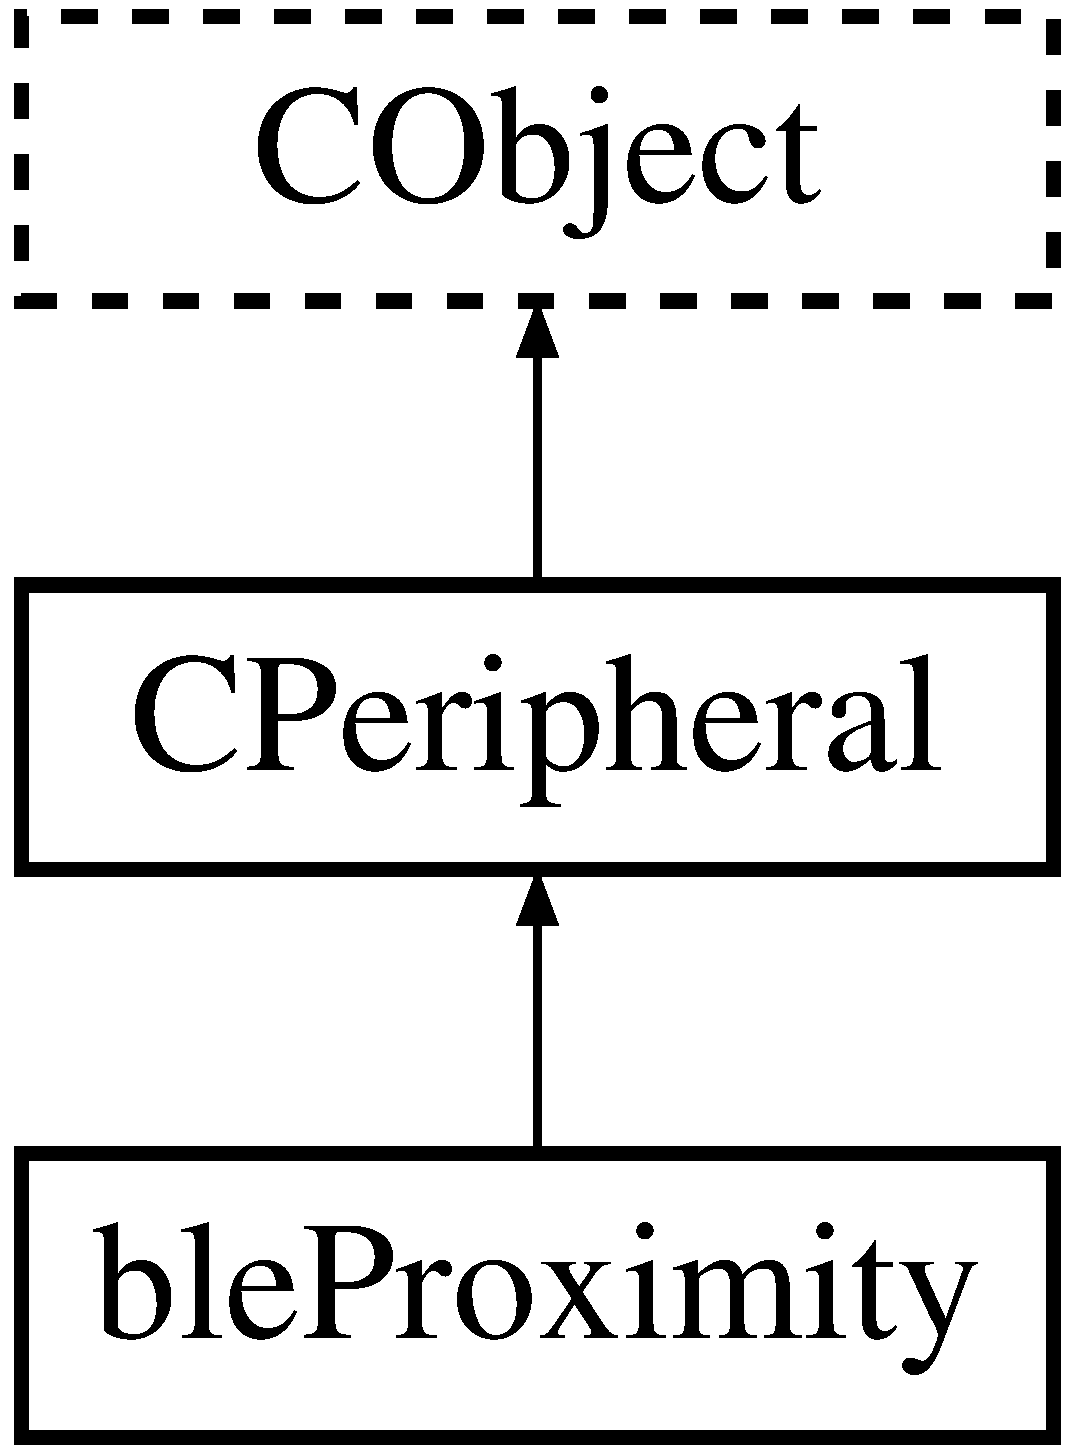
\includegraphics[height=3.000000cm]{de/d67/classble_proximity}
\end{center}
\end{figure}
\subsection*{Public Member Functions}
\begin{DoxyCompactItemize}
\item 
\hyperlink{classble_proximity_a3cbf3bd31cac77037d623ef9c8098a71}{ble\-Proximity} (\hyperlink{classble_serial}{ble\-Serial} \&ble)
\item 
virtual void \hyperlink{classble_proximity_a43c9187ddcb7237099ff414b74c5b0bd}{on\-Alert} (uint8\-\_\-t level)
\item 
virtual void \hyperlink{classble_proximity_a193eb5410fc4cf4b35613ad931ae61ff}{on\-Link\-Loss} (uint8\-\_\-t level)
\item 
virtual bool \hyperlink{classble_proximity_a6d3426d21b9182c5b3e135dd783e097d}{send\-Event} (uint8\-\_\-t level)
\item 
virtual void \hyperlink{classble_proximity_a177463a01974a439c9f8d90b36cf15e1}{set\-Tx\-Power\-Level} (int8\-\_\-t d\-Bm)
\item 
virtual bool \hyperlink{classble_proximity_adc2ab90789ee61d11031ce816b3db11c}{is\-Available} ()
\end{DoxyCompactItemize}


\subsection{Detailed Description}
\hyperlink{classble_proximity}{ble\-Proximity} provide \char`\"{}\-Immediate Alert\char`\"{} and \char`\"{}\-Link Loss\char`\"{} services. The \hyperlink{classble_proximity}{ble\-Proximity} enables proximity monitoring between two devices.\par
 See Also\-:\par
 \href{https://developer.bluetooth.org/TechnologyOverview/Pages/PXP.aspx}{\tt Proximity Profile (P\-X\-P)} 

\subsection{Constructor \& Destructor Documentation}
\hypertarget{classble_proximity_a3cbf3bd31cac77037d623ef9c8098a71}{\index{ble\-Proximity@{ble\-Proximity}!ble\-Proximity@{ble\-Proximity}}
\index{ble\-Proximity@{ble\-Proximity}!bleProximity@{ble\-Proximity}}
\subsubsection[{ble\-Proximity}]{\setlength{\rightskip}{0pt plus 5cm}ble\-Proximity\-::ble\-Proximity (
\begin{DoxyParamCaption}
\item[{{\bf ble\-Serial} \&}]{ble}
\end{DoxyParamCaption}
)}}\label{classble_proximity_a3cbf3bd31cac77037d623ef9c8098a71}
\hyperlink{classble_proximity}{ble\-Proximity} constructor. 
\begin{DoxyParams}[1]{Parameters}
\mbox{\tt in}  & {\em ble} & is a \hyperlink{classble_serial}{ble\-Serial} class object. \\
\hline
\end{DoxyParams}


\subsection{Member Function Documentation}
\hypertarget{classble_proximity_a43c9187ddcb7237099ff414b74c5b0bd}{\index{ble\-Proximity@{ble\-Proximity}!on\-Alert@{on\-Alert}}
\index{on\-Alert@{on\-Alert}!bleProximity@{ble\-Proximity}}
\subsubsection[{on\-Alert}]{\setlength{\rightskip}{0pt plus 5cm}virtual void ble\-Proximity\-::on\-Alert (
\begin{DoxyParamCaption}
\item[{uint8\-\_\-t}]{level}
\end{DoxyParamCaption}
)\hspace{0.3cm}{\ttfamily [virtual]}}}\label{classble_proximity_a43c9187ddcb7237099ff414b74c5b0bd}
on\-Alert event is call by B\-L\-E task. 
\begin{DoxyParams}[1]{Parameters}
\mbox{\tt in}  & {\em level} & is an uint8\-\_\-t type value, 0=No Alert, 1=Mild Alert, 2=High Alert, 3-\/255 reserved. \\
\hline
\end{DoxyParams}
\begin{DoxyRemark}{Remarks}
The on\-Alert will be implemented by the \hyperlink{classble_proximity}{ble\-Proximity} class. 
\end{DoxyRemark}
\begin{DoxyNote}{Note}
The event is defined in the Immediate service of B\-L\-E. The Alert Level characteristic is a control point that allows a peer to command this device to alert to a given level. 
\end{DoxyNote}
\hypertarget{classble_proximity_a193eb5410fc4cf4b35613ad931ae61ff}{\index{ble\-Proximity@{ble\-Proximity}!on\-Link\-Loss@{on\-Link\-Loss}}
\index{on\-Link\-Loss@{on\-Link\-Loss}!bleProximity@{ble\-Proximity}}
\subsubsection[{on\-Link\-Loss}]{\setlength{\rightskip}{0pt plus 5cm}virtual void ble\-Proximity\-::on\-Link\-Loss (
\begin{DoxyParamCaption}
\item[{uint8\-\_\-t}]{level}
\end{DoxyParamCaption}
)\hspace{0.3cm}{\ttfamily [virtual]}}}\label{classble_proximity_a193eb5410fc4cf4b35613ad931ae61ff}
on\-Link\-Loss event is call by B\-L\-E task. 
\begin{DoxyParams}{Parameters}
{\em level} & is an uint8\-\_\-t type value, 0=No Alert, 1=Mild Alert, 2=High Alert, 3-\/255 reserved. \\
\hline
\end{DoxyParams}
\begin{DoxyRemark}{Remarks}
The on\-Link\-Lose will be implemented by the ble\-Proxmity class. 
\end{DoxyRemark}
\begin{DoxyNote}{Note}
The event is defined in the Link-\/\-Lose service of B\-L\-E. The Alert Level characteristic is used to expose the current link loss alert level that is used to determine how the device alerts when the link is lost. 
\end{DoxyNote}
\hypertarget{classble_proximity_a6d3426d21b9182c5b3e135dd783e097d}{\index{ble\-Proximity@{ble\-Proximity}!send\-Event@{send\-Event}}
\index{send\-Event@{send\-Event}!bleProximity@{ble\-Proximity}}
\subsubsection[{send\-Event}]{\setlength{\rightskip}{0pt plus 5cm}virtual bool ble\-Proximity\-::send\-Event (
\begin{DoxyParamCaption}
\item[{uint8\-\_\-t}]{level}
\end{DoxyParamCaption}
)\hspace{0.3cm}{\ttfamily [virtual]}}}\label{classble_proximity_a6d3426d21b9182c5b3e135dd783e097d}
Send alert event to remote (App). 
\begin{DoxyParams}[1]{Parameters}
\mbox{\tt in}  & {\em level} & is an uint8\-\_\-t type value to indicate B\-L\-E devie alert level. \\
\hline
\end{DoxyParams}
\begin{DoxyReturn}{Returns}
true, if send alert event successful. otherwise, if send alert event failed. 
\end{DoxyReturn}
\hypertarget{classble_proximity_a177463a01974a439c9f8d90b36cf15e1}{\index{ble\-Proximity@{ble\-Proximity}!set\-Tx\-Power\-Level@{set\-Tx\-Power\-Level}}
\index{set\-Tx\-Power\-Level@{set\-Tx\-Power\-Level}!bleProximity@{ble\-Proximity}}
\subsubsection[{set\-Tx\-Power\-Level}]{\setlength{\rightskip}{0pt plus 5cm}virtual void ble\-Proximity\-::set\-Tx\-Power\-Level (
\begin{DoxyParamCaption}
\item[{int8\-\_\-t}]{d\-Bm}
\end{DoxyParamCaption}
)\hspace{0.3cm}{\ttfamily [virtual]}}}\label{classble_proximity_a177463a01974a439c9f8d90b36cf15e1}
set\-Tx\-Power\-Level exposes a device’s current transmit power level when in a connection. 
\begin{DoxyParams}[1]{Parameters}
\mbox{\tt in}  & {\em d\-Bm} & is a signed integer and range from +20d\-Bm to -\/120d\-Bm \\
\hline
\end{DoxyParams}
\hypertarget{classble_proximity_adc2ab90789ee61d11031ce816b3db11c}{\index{ble\-Proximity@{ble\-Proximity}!is\-Available@{is\-Available}}
\index{is\-Available@{is\-Available}!bleProximity@{ble\-Proximity}}
\subsubsection[{is\-Available}]{\setlength{\rightskip}{0pt plus 5cm}virtual bool ble\-Proximity\-::is\-Available (
\begin{DoxyParamCaption}
{}
\end{DoxyParamCaption}
)\hspace{0.3cm}{\ttfamily [virtual]}}}\label{classble_proximity_adc2ab90789ee61d11031ce816b3db11c}
Use is\-Available to check the service whether opened by remote (App). \begin{DoxyReturn}{Returns}
true, if service is available. otherwise, the service is not in used. 
\end{DoxyReturn}


The documentation for this class was generated from the following file\-:\begin{DoxyCompactItemize}
\item 
ble\-\_\-proximity.\-h\end{DoxyCompactItemize}

\hypertarget{classble_serial}{\section{ble\-Serial Class Reference}
\label{classble_serial}\index{ble\-Serial@{ble\-Serial}}
}


\hyperlink{classble_serial}{ble\-Serial} class is a ble core, and inherit from \hyperlink{class_c_stream}{C\-Stream} class to provide the stream virtual functions for serial input and output. the \hyperlink{classble_serial}{ble\-Serial} class also inherit from the \hyperlink{class_c_thread}{C\-Thread} class and can work in background.  




{\ttfamily \#include \char`\"{}class/ble\-\_\-serial.\-h\char`\"{}}

Inheritance diagram for ble\-Serial\-:\begin{figure}[H]
\begin{center}
\leavevmode
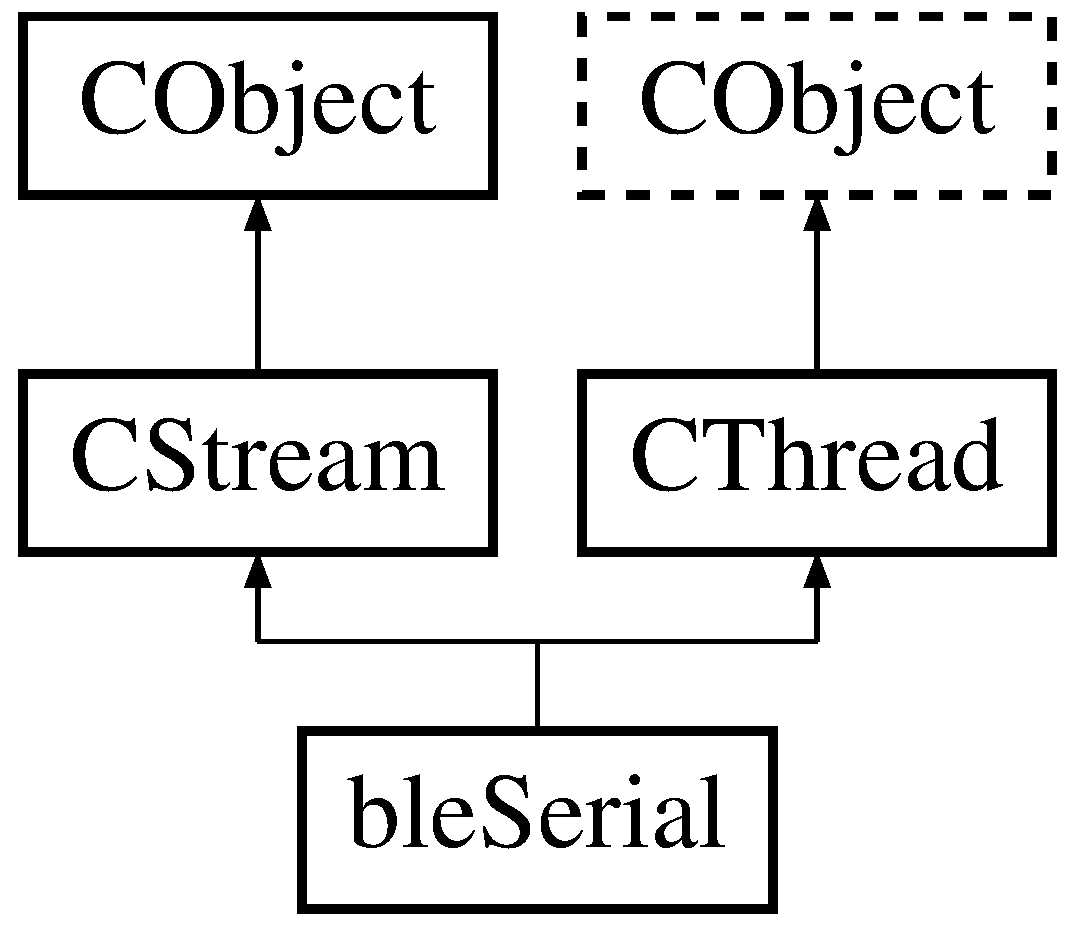
\includegraphics[height=3.000000cm]{d7/d03/classble_serial}
\end{center}
\end{figure}
\subsection*{Public Member Functions}
\begin{DoxyCompactItemize}
\item 
\hyperlink{classble_serial_a835c884c9209b074cf82e5a3f0a322ec}{ble\-Serial} (L\-P\-C\-T\-S\-T\-R device\-Name=D\-E\-F\-\_\-\-B\-L\-E\-\_\-\-D\-E\-V\-I\-C\-E\-N\-A\-M\-E)
\begin{DoxyCompactList}\small\item\em \hyperlink{classble_serial}{ble\-Serial} constructor with a G\-A\-T device name. \end{DoxyCompactList}\item 
void \hyperlink{classble_serial_a0ee4ea2d6d4a38bbd64968336f85c2e9}{advertising} (uint16\-\_\-t adv\-Interval, int8\-\_\-t tx\-Power\-Level=D\-E\-F\-\_\-\-B\-L\-E\-\_\-\-T\-X\-P\-O\-W\-E\-R, uint16\-\_\-t conn\-Interval=D\-E\-F\-\_\-\-B\-L\-E\-\_\-\-C\-O\-N\-N\-\_\-\-I\-N\-T\-E\-R\-V\-A\-L, uint16\-\_\-t conn\-Timeout=D\-E\-F\-\_\-\-B\-L\-E\-\_\-\-C\-O\-N\-N\-\_\-\-T\-I\-M\-E\-O\-U\-T, uint16\-\_\-t manufacture\-Data=D\-E\-F\-\_\-\-B\-L\-E\-\_\-\-M\-F\-G\-\_\-\-D\-A\-T\-A)
\item 
void \hyperlink{classble_serial_acc1e214474c9e98705fb7f363a3eee74}{setup} (uint16\-\_\-t adv\-Interval, int8\-\_\-t tx\-Power\-Level=D\-E\-F\-\_\-\-B\-L\-E\-\_\-\-T\-X\-P\-O\-W\-E\-R, uint16\-\_\-t conn\-Interval=D\-E\-F\-\_\-\-B\-L\-E\-\_\-\-C\-O\-N\-N\-\_\-\-I\-N\-T\-E\-R\-V\-A\-L, uint16\-\_\-t conn\-Timeout=D\-E\-F\-\_\-\-B\-L\-E\-\_\-\-C\-O\-N\-N\-\_\-\-T\-I\-M\-E\-O\-U\-T, uint16\-\_\-t manufacture\-Data=D\-E\-F\-\_\-\-B\-L\-E\-\_\-\-M\-F\-G\-\_\-\-D\-A\-T\-A)
\item 
bool \hyperlink{classble_serial_a3ff1e4b271a7d225e73abd337043d8e4}{enable} (uint32\-\_\-t stack=128)
\item 
void \hyperlink{classble_serial_a08b3a82e95aa527433c04b4a6a3d81d4}{disable} ()
\item 
void \hyperlink{classble_serial_a4188fc1bab7e077cf1d573024f092c7b}{poll\-Interval} (uint32\-\_\-t ms)
\item 
void \hyperlink{classble_serial_a2588b21bf80d35a866dc7e47f97142df}{watchdog} (uint32\-\_\-t tm)
\item 
bool \hyperlink{classble_serial_ab766015c18f219e359edc1c560d66893}{is\-Actived} ()
\item 
bool \hyperlink{classble_serial_a5e63823fd7ff0ef0ac5447cd265b5a5c}{disconnect} (\hyperlink{group___enumerations_gafdc7d73c1364c4d42f80cfdc702de294}{B\-L\-E\-\_\-\-D\-I\-S\-C\-O\-N\-N\-E\-C\-T\-\_\-\-R\-E\-A\-S\-O\-N\-\_\-\-T} reason=\hyperlink{group___enumerations_ggafdc7d73c1364c4d42f80cfdc702de294a3aaba90cbef710f140a4f7e70d1f0d5b}{B\-L\-E\-\_\-\-T\-E\-R\-M\-I\-N\-A\-T\-E\-D})
\item 
bool \hyperlink{classble_serial_acddad359ad714bd31358c96966839a61}{set\-Radio\-Tx\-Power} (\hyperlink{group___enumerations_ga3b6d6db9e13e93ae21f2a383d9903617}{B\-L\-E\-\_\-\-T\-X\-\_\-\-P\-O\-W\-E\-R\-\_\-\-T} power)
\item 
uint8\-\_\-t \hyperlink{classble_serial_a6aea16b265aa98f0a540f71b75965408}{get\-Phy\-Version} ()
\item 
virtual void \hyperlink{classble_serial_adb930ce55295ff7eb6ab5bdbeb702749}{on\-Connected} ()
\item 
virtual void \hyperlink{classble_serial_aa6f5116c8bcf05011a05ad5e2967c318}{on\-Disconnected} ()
\item 
virtual void \hyperlink{classble_serial_a8af315789cc459a1fde96ac80ca9ffb7}{on\-Watchdog} ()
\item 
virtual void \hyperlink{classble_serial_a8a0622f5d10fe2242978a16b2d1e6ee4}{on\-Error} (\hyperlink{group___enumerations_ga6c00522f6a8c33135ee0414877d42c04}{B\-L\-E\-\_\-\-E\-R\-R\-\_\-\-T} err, L\-P\-C\-T\-S\-T\-R id=\char`\"{}ble\-Serial\char`\"{})
\item 
bool \hyperlink{classble_serial_a1691c5c5655043512bf1c462e6928488}{is\-Available} ()
\item 
virtual int \hyperlink{classble_serial_a59dca8e3e2d6945a699347f4c4708fd4}{readable} ()
\item 
virtual int \hyperlink{classble_serial_ac42a8f805e6784e0fa2064270b5288a1}{writeable} ()
\item 
virtual int \hyperlink{classble_serial_a186e09706d9b6e58a6213ac0b6a220ad}{read} (void $\ast$buf, int len, bool block=true)
\item 
virtual int \hyperlink{classble_serial_ab9d147e7dcb9436f390f2ad29d539930}{write} (const void $\ast$buf, int len, bool block=true)
\item 
virtual bool \hyperlink{classble_serial_aebfde0d9a7583cb641ac60f02df7cd77}{is\-Connected} ()
\item 
virtual void \hyperlink{classble_serial_ad41b78cc1b0fc02ce65248147b32ffa8}{flush} ()
\end{DoxyCompactItemize}
\subsection*{Additional Inherited Members}


\subsection{Detailed Description}
\hyperlink{classble_serial}{ble\-Serial} class is a ble core, and inherit from \hyperlink{class_c_stream}{C\-Stream} class to provide the stream virtual functions for serial input and output. the \hyperlink{classble_serial}{ble\-Serial} class also inherit from the \hyperlink{class_c_thread}{C\-Thread} class and can work in background. 

\subsection{Constructor \& Destructor Documentation}
\hypertarget{classble_serial_a835c884c9209b074cf82e5a3f0a322ec}{\index{ble\-Serial@{ble\-Serial}!ble\-Serial@{ble\-Serial}}
\index{ble\-Serial@{ble\-Serial}!bleSerial@{ble\-Serial}}
\subsubsection[{ble\-Serial}]{\setlength{\rightskip}{0pt plus 5cm}ble\-Serial\-::ble\-Serial (
\begin{DoxyParamCaption}
\item[{L\-P\-C\-T\-S\-T\-R}]{device\-Name = {\ttfamily DEF\-\_\-BLE\-\_\-DEVICENAME}}
\end{DoxyParamCaption}
)}}\label{classble_serial_a835c884c9209b074cf82e5a3f0a322ec}


\hyperlink{classble_serial}{ble\-Serial} constructor with a G\-A\-T device name. 

\hyperlink{classble_serial}{ble\-Serial} constructor 
\begin{DoxyCode}
\textcolor{keywordtype}{int} main() \{
        ...
        \hyperlink{classble_serial}{bleSerial} ble(\textcolor{stringliteral}{"myBLE"});
        ble.advertising(100);   \textcolor{comment}{// set advertising interval 100ms}
        ble.enable();
        ...
        ...
\end{DoxyCode}
 
\begin{DoxyParams}{Parameters}
{\em device\-Name} & point to a L\-P\-C\-T\-S\-T\-R string to indicate the G\-A\-T device name of Bluetooth. \\
\hline
\end{DoxyParams}


\subsection{Member Function Documentation}
\hypertarget{classble_serial_a0ee4ea2d6d4a38bbd64968336f85c2e9}{\index{ble\-Serial@{ble\-Serial}!advertising@{advertising}}
\index{advertising@{advertising}!bleSerial@{ble\-Serial}}
\subsubsection[{advertising}]{\setlength{\rightskip}{0pt plus 5cm}void ble\-Serial\-::advertising (
\begin{DoxyParamCaption}
\item[{uint16\-\_\-t}]{adv\-Interval, }
\item[{int8\-\_\-t}]{tx\-Power\-Level = {\ttfamily DEF\-\_\-BLE\-\_\-TXPOWER}, }
\item[{uint16\-\_\-t}]{conn\-Interval = {\ttfamily DEF\-\_\-BLE\-\_\-CONN\-\_\-INTERVAL}, }
\item[{uint16\-\_\-t}]{conn\-Timeout = {\ttfamily DEF\-\_\-BLE\-\_\-CONN\-\_\-TIMEOUT}, }
\item[{uint16\-\_\-t}]{manufacture\-Data = {\ttfamily DEF\-\_\-BLE\-\_\-MFG\-\_\-DATA}}
\end{DoxyParamCaption}
)}}\label{classble_serial_a0ee4ea2d6d4a38bbd64968336f85c2e9}
Broadcast the advertising message when device is not in B\-L\-E connection. 
\begin{DoxyParams}{Parameters}
{\em adv\-Interval} & To broadcast the advertising message with the interval time in millisecond. \\
\hline
{\em tx\-Power\-Level} & To expose the \char`\"{}\-Tx\-Power\-Level\char`\"{} on the advertising message. \\
\hline
{\em conn\-Interval} & To expose the \char`\"{}connection interval\char`\"{} on the advertising message. \\
\hline
{\em conn\-Timeout} & To expose the \char`\"{}connection timeout\char`\"{} on the advertising message. \\
\hline
{\em manufacture\-Data} & To expose the \char`\"{}\-Manufacture Data\char`\"{} on the advertising message. \\
\hline
\end{DoxyParams}
\begin{DoxyRemark}{Remarks}
advertising(...) have to call before the \hyperlink{classble_serial_a3ff1e4b271a7d225e73abd337043d8e4}{enable()} member. 
\end{DoxyRemark}
\begin{DoxySeeAlso}{See Also}
\hyperlink{classble_serial_a835c884c9209b074cf82e5a3f0a322ec}{ble\-Serial()} 
\end{DoxySeeAlso}
\hypertarget{classble_serial_acc1e214474c9e98705fb7f363a3eee74}{\index{ble\-Serial@{ble\-Serial}!setup@{setup}}
\index{setup@{setup}!bleSerial@{ble\-Serial}}
\subsubsection[{setup}]{\setlength{\rightskip}{0pt plus 5cm}void ble\-Serial\-::setup (
\begin{DoxyParamCaption}
\item[{uint16\-\_\-t}]{adv\-Interval, }
\item[{int8\-\_\-t}]{tx\-Power\-Level = {\ttfamily DEF\-\_\-BLE\-\_\-TXPOWER}, }
\item[{uint16\-\_\-t}]{conn\-Interval = {\ttfamily DEF\-\_\-BLE\-\_\-CONN\-\_\-INTERVAL}, }
\item[{uint16\-\_\-t}]{conn\-Timeout = {\ttfamily DEF\-\_\-BLE\-\_\-CONN\-\_\-TIMEOUT}, }
\item[{uint16\-\_\-t}]{manufacture\-Data = {\ttfamily DEF\-\_\-BLE\-\_\-MFG\-\_\-DATA}}
\end{DoxyParamCaption}
)\hspace{0.3cm}{\ttfamily [inline]}}}\label{classble_serial_acc1e214474c9e98705fb7f363a3eee74}
An inline function redirect to \hyperlink{classble_serial_a0ee4ea2d6d4a38bbd64968336f85c2e9}{advertising()} member function. \begin{DoxySeeAlso}{See Also}
\hyperlink{classble_serial_a0ee4ea2d6d4a38bbd64968336f85c2e9}{advertising} 
\end{DoxySeeAlso}
\hypertarget{classble_serial_a3ff1e4b271a7d225e73abd337043d8e4}{\index{ble\-Serial@{ble\-Serial}!enable@{enable}}
\index{enable@{enable}!bleSerial@{ble\-Serial}}
\subsubsection[{enable}]{\setlength{\rightskip}{0pt plus 5cm}bool ble\-Serial\-::enable (
\begin{DoxyParamCaption}
\item[{uint32\-\_\-t}]{stack = {\ttfamily 128}}
\end{DoxyParamCaption}
)}}\label{classble_serial_a3ff1e4b271a7d225e73abd337043d8e4}
The enable member is to call the \hyperlink{class_c_thread}{C\-Thread}\-:\hyperlink{class_c_thread_aacf955d1852e74da1f989251955ee6ec}{start()} to start the ble engine task. 
\begin{DoxyCode}
\textcolor{preprocessor}{#include "class/ble\_serial.h"}
\textcolor{keywordtype}{int} main() \{
        \hyperlink{classble_serial}{bleSerial} ble(\textcolor{stringliteral}{"myBLE"});
        ble.enable();   \textcolor{comment}{// to start the BLE core and Task.}
        ...
        ...
\}
\end{DoxyCode}
 
\begin{DoxyParams}{Parameters}
{\em stack} & To indicate the stack size of B\-L\-E task. default is 128 bytes. \\
\hline
\end{DoxyParams}
\begin{DoxyReturn}{Returns}
true if start the ble task successful, otherwise is failed. 
\end{DoxyReturn}
\hypertarget{classble_serial_a08b3a82e95aa527433c04b4a6a3d81d4}{\index{ble\-Serial@{ble\-Serial}!disable@{disable}}
\index{disable@{disable}!bleSerial@{ble\-Serial}}
\subsubsection[{disable}]{\setlength{\rightskip}{0pt plus 5cm}void ble\-Serial\-::disable (
\begin{DoxyParamCaption}
{}
\end{DoxyParamCaption}
)}}\label{classble_serial_a08b3a82e95aa527433c04b4a6a3d81d4}
The disable member is to suspend the ble\-Serail task. \begin{DoxyNote}{Note}
Call enable member to resume the ble\-Serail task. 
\end{DoxyNote}
\hypertarget{classble_serial_a4188fc1bab7e077cf1d573024f092c7b}{\index{ble\-Serial@{ble\-Serial}!poll\-Interval@{poll\-Interval}}
\index{poll\-Interval@{poll\-Interval}!bleSerial@{ble\-Serial}}
\subsubsection[{poll\-Interval}]{\setlength{\rightskip}{0pt plus 5cm}void ble\-Serial\-::poll\-Interval (
\begin{DoxyParamCaption}
\item[{uint32\-\_\-t}]{ms}
\end{DoxyParamCaption}
)}}\label{classble_serial_a4188fc1bab7e077cf1d573024f092c7b}
Poll the B\-L\-E core with the interval time in milliseconds. 
\begin{DoxyParams}{Parameters}
{\em ms} & A millisecond value. \\
\hline
\end{DoxyParams}
\begin{DoxyNote}{Note}
The member is a optional function, and default is 50ms. 
\end{DoxyNote}
\hypertarget{classble_serial_a2588b21bf80d35a866dc7e47f97142df}{\index{ble\-Serial@{ble\-Serial}!watchdog@{watchdog}}
\index{watchdog@{watchdog}!bleSerial@{ble\-Serial}}
\subsubsection[{watchdog}]{\setlength{\rightskip}{0pt plus 5cm}void ble\-Serial\-::watchdog (
\begin{DoxyParamCaption}
\item[{uint32\-\_\-t}]{tm}
\end{DoxyParamCaption}
)}}\label{classble_serial_a2588b21bf80d35a866dc7e47f97142df}
Enable a watchdog on a B\-L\-E connection. The watchdog feature will cause the B\-L\-E core reset when remote (App) crash or lose the connection. 
\begin{DoxyParams}{Parameters}
{\em tm} & A timeout value in millisecond, recommend value is 500$\sim$30000. If set the tm to zero, it is meant to disable the watchdog. \\
\hline
\end{DoxyParams}
\begin{DoxyNote}{Note}
The member is an optional function, and default is 10,000ms (10 seconds). 
\end{DoxyNote}
\hypertarget{classble_serial_ab766015c18f219e359edc1c560d66893}{\index{ble\-Serial@{ble\-Serial}!is\-Actived@{is\-Actived}}
\index{is\-Actived@{is\-Actived}!bleSerial@{ble\-Serial}}
\subsubsection[{is\-Actived}]{\setlength{\rightskip}{0pt plus 5cm}bool ble\-Serial\-::is\-Actived (
\begin{DoxyParamCaption}
{}
\end{DoxyParamCaption}
)}}\label{classble_serial_ab766015c18f219e359edc1c560d66893}
To check that radio is activated before the radio becomes active. \begin{DoxyReturn}{Returns}
true if the radio is activated, otherwise if the radio is inactivated. 
\end{DoxyReturn}
\hypertarget{classble_serial_a5e63823fd7ff0ef0ac5447cd265b5a5c}{\index{ble\-Serial@{ble\-Serial}!disconnect@{disconnect}}
\index{disconnect@{disconnect}!bleSerial@{ble\-Serial}}
\subsubsection[{disconnect}]{\setlength{\rightskip}{0pt plus 5cm}bool ble\-Serial\-::disconnect (
\begin{DoxyParamCaption}
\item[{{\bf B\-L\-E\-\_\-\-D\-I\-S\-C\-O\-N\-N\-E\-C\-T\-\_\-\-R\-E\-A\-S\-O\-N\-\_\-\-T}}]{reason = {\ttfamily {\bf B\-L\-E\-\_\-\-T\-E\-R\-M\-I\-N\-A\-T\-E\-D}}}
\end{DoxyParamCaption}
)}}\label{classble_serial_a5e63823fd7ff0ef0ac5447cd265b5a5c}
To disconnect current connection with a reason. 
\begin{DoxyParams}{Parameters}
{\em reason} & is a B\-L\-E\-\_\-\-D\-I\-S\-C\-O\-N\-N\-E\-C\-T\-\_\-\-R\-E\-A\-S\-O\-N\-\_\-\-T enumeration. \\
\hline
\end{DoxyParams}
\begin{DoxyReturn}{Returns}
true if disconnect successful, otherwise, disconnect failed. 
\end{DoxyReturn}
\hypertarget{classble_serial_acddad359ad714bd31358c96966839a61}{\index{ble\-Serial@{ble\-Serial}!set\-Radio\-Tx\-Power@{set\-Radio\-Tx\-Power}}
\index{set\-Radio\-Tx\-Power@{set\-Radio\-Tx\-Power}!bleSerial@{ble\-Serial}}
\subsubsection[{set\-Radio\-Tx\-Power}]{\setlength{\rightskip}{0pt plus 5cm}bool ble\-Serial\-::set\-Radio\-Tx\-Power (
\begin{DoxyParamCaption}
\item[{{\bf B\-L\-E\-\_\-\-T\-X\-\_\-\-P\-O\-W\-E\-R\-\_\-\-T}}]{power}
\end{DoxyParamCaption}
)}}\label{classble_serial_acddad359ad714bd31358c96966839a61}
Set the ouptut power level of the Bluetooth Low Energy radio. 
\begin{DoxyParams}{Parameters}
{\em power} & is a B\-L\-E\-\_\-\-T\-X\-\_\-\-P\-O\-W\-E\-R\-\_\-\-T enumeration. \\
\hline
\end{DoxyParams}
\begin{DoxyReturn}{Returns}
true if set radio power successful, otherwise is failed. 
\end{DoxyReturn}
\hypertarget{classble_serial_a6aea16b265aa98f0a540f71b75965408}{\index{ble\-Serial@{ble\-Serial}!get\-Phy\-Version@{get\-Phy\-Version}}
\index{get\-Phy\-Version@{get\-Phy\-Version}!bleSerial@{ble\-Serial}}
\subsubsection[{get\-Phy\-Version}]{\setlength{\rightskip}{0pt plus 5cm}uint8\-\_\-t ble\-Serial\-::get\-Phy\-Version (
\begin{DoxyParamCaption}
{}
\end{DoxyParamCaption}
)}}\label{classble_serial_a6aea16b265aa98f0a540f71b75965408}
Get B\-L\-E core hardware version. \begin{DoxyReturn}{Returns}
An uint8\-\_\-t type value. 
\end{DoxyReturn}
\hypertarget{classble_serial_adb930ce55295ff7eb6ab5bdbeb702749}{\index{ble\-Serial@{ble\-Serial}!on\-Connected@{on\-Connected}}
\index{on\-Connected@{on\-Connected}!bleSerial@{ble\-Serial}}
\subsubsection[{on\-Connected}]{\setlength{\rightskip}{0pt plus 5cm}virtual void ble\-Serial\-::on\-Connected (
\begin{DoxyParamCaption}
{}
\end{DoxyParamCaption}
)\hspace{0.3cm}{\ttfamily [virtual]}}}\label{classble_serial_adb930ce55295ff7eb6ab5bdbeb702749}
An virtual function call by B\-L\-E task and occurs when remote (App) is already to connect the B\-L\-E device. \begin{DoxyRemark}{Remarks}
To override the virtual, the on\-Connection of child have to call the on\-Connection of supper class. 
\begin{DoxyCode}
\textcolor{keyword}{class }myBle: \textcolor{keyword}{public} \hyperlink{classble_serial}{bleSerial} \{
\textcolor{keyword}{public}:
        \textcolor{comment}{// override the onConnected() virtual function}
        \textcolor{keyword}{virtual} \hyperlink{classble_serial_adb930ce55295ff7eb6ab5bdbeb702749}{onConnected}() \{
            bleSerial::onConnection();      \textcolor{comment}{// call to parent class}

            \textcolor{comment}{// your onConnection event code here:}
            ...
            ...
        \}
    \};
\end{DoxyCode}
 
\end{DoxyRemark}
\hypertarget{classble_serial_aa6f5116c8bcf05011a05ad5e2967c318}{\index{ble\-Serial@{ble\-Serial}!on\-Disconnected@{on\-Disconnected}}
\index{on\-Disconnected@{on\-Disconnected}!bleSerial@{ble\-Serial}}
\subsubsection[{on\-Disconnected}]{\setlength{\rightskip}{0pt plus 5cm}virtual void ble\-Serial\-::on\-Disconnected (
\begin{DoxyParamCaption}
{}
\end{DoxyParamCaption}
)\hspace{0.3cm}{\ttfamily [virtual]}}}\label{classble_serial_aa6f5116c8bcf05011a05ad5e2967c318}
An virtual function call by B\-L\-E task and occurs when remote (App) is already to disconnect the B\-L\-E device. \begin{DoxyRemark}{Remarks}
To override the virtual, the on\-Disconnection of child have to call the on\-Disconnection of parent class. 
\begin{DoxyCode}
\textcolor{keyword}{class }myBle: \textcolor{keyword}{public} \hyperlink{classble_serial}{bleSerial} \{
\textcolor{keyword}{public}:
        \textcolor{comment}{// override the onConnected() virtual function}
        \textcolor{keyword}{virtual} \hyperlink{classble_serial_aa6f5116c8bcf05011a05ad5e2967c318}{onDisconnected}() \{
            bleSerial::onDisconnection();   \textcolor{comment}{// call to parent class}

            \textcolor{comment}{// your onDisonnection event code here:}
            ...
            ...
        \}
    \};
\end{DoxyCode}
 
\end{DoxyRemark}
\hypertarget{classble_serial_a8af315789cc459a1fde96ac80ca9ffb7}{\index{ble\-Serial@{ble\-Serial}!on\-Watchdog@{on\-Watchdog}}
\index{on\-Watchdog@{on\-Watchdog}!bleSerial@{ble\-Serial}}
\subsubsection[{on\-Watchdog}]{\setlength{\rightskip}{0pt plus 5cm}virtual void ble\-Serial\-::on\-Watchdog (
\begin{DoxyParamCaption}
{}
\end{DoxyParamCaption}
)\hspace{0.3cm}{\ttfamily [virtual]}}}\label{classble_serial_a8af315789cc459a1fde96ac80ca9ffb7}
An virtual function call by B\-L\-E task and occurs when a watchdog timeout on a connection. \begin{DoxyRemark}{Remarks}
The on\-Watchdog member will call the reset() member function to reset the B\-L\-E core. 
\end{DoxyRemark}
\hypertarget{classble_serial_a8a0622f5d10fe2242978a16b2d1e6ee4}{\index{ble\-Serial@{ble\-Serial}!on\-Error@{on\-Error}}
\index{on\-Error@{on\-Error}!bleSerial@{ble\-Serial}}
\subsubsection[{on\-Error}]{\setlength{\rightskip}{0pt plus 5cm}virtual void ble\-Serial\-::on\-Error (
\begin{DoxyParamCaption}
\item[{{\bf B\-L\-E\-\_\-\-E\-R\-R\-\_\-\-T}}]{err, }
\item[{L\-P\-C\-T\-S\-T\-R}]{id = {\ttfamily \char`\"{}bleSerial\char`\"{}}}
\end{DoxyParamCaption}
)\hspace{0.3cm}{\ttfamily [inline]}, {\ttfamily [virtual]}}}\label{classble_serial_a8a0622f5d10fe2242978a16b2d1e6ee4}
An virtual function call by B\-L\-E task and occurs when a B\-L\-E hardware error. 
\begin{DoxyParams}{Parameters}
{\em error} & A B\-L\-E\-\_\-\-E\-R\-R\-\_\-\-T enumeration. \\
\hline
{\em id} & A string to a class name. (for debug) \\
\hline
\end{DoxyParams}
\begin{DoxyNote}{Note}
The on\-Error event is a empty function in \hyperlink{classble_serial}{ble\-Serial} class. 
\end{DoxyNote}
\hypertarget{classble_serial_a1691c5c5655043512bf1c462e6928488}{\index{ble\-Serial@{ble\-Serial}!is\-Available@{is\-Available}}
\index{is\-Available@{is\-Available}!bleSerial@{ble\-Serial}}
\subsubsection[{is\-Available}]{\setlength{\rightskip}{0pt plus 5cm}bool ble\-Serial\-::is\-Available (
\begin{DoxyParamCaption}
{}
\end{DoxyParamCaption}
)\hspace{0.3cm}{\ttfamily [inline]}}}\label{classble_serial_a1691c5c5655043512bf1c462e6928488}
Use is\-Available to check the service whether opened by remote (App). \begin{DoxyReturn}{Returns}
true, if service is available. otherwise, the service is not in used. 
\end{DoxyReturn}
\begin{DoxyNote}{Note}
This is\-Available member is an inline function to redirect to the \hyperlink{classble_serial_ac42a8f805e6784e0fa2064270b5288a1}{writeable()} member. 
\end{DoxyNote}
\begin{DoxySeeAlso}{See Also}
\hyperlink{classble_serial_ac42a8f805e6784e0fa2064270b5288a1}{writeable} 
\end{DoxySeeAlso}
\hypertarget{classble_serial_a59dca8e3e2d6945a699347f4c4708fd4}{\index{ble\-Serial@{ble\-Serial}!readable@{readable}}
\index{readable@{readable}!bleSerial@{ble\-Serial}}
\subsubsection[{readable}]{\setlength{\rightskip}{0pt plus 5cm}virtual int ble\-Serial\-::readable (
\begin{DoxyParamCaption}
{}
\end{DoxyParamCaption}
)\hspace{0.3cm}{\ttfamily [virtual]}}}\label{classble_serial_a59dca8e3e2d6945a699347f4c4708fd4}
Determine how many data bytes are available to read. \begin{DoxyReturn}{Returns}
A value to indicate how many data byte is available in the input buffer. 
\end{DoxyReturn}
\begin{DoxyRemark}{Remarks}
the pure virtual function have to implement by child class. 
\end{DoxyRemark}


Reimplemented from \hyperlink{class_c_stream_a96328807241e15017868b845b06fd9e4}{C\-Stream}.

\hypertarget{classble_serial_ac42a8f805e6784e0fa2064270b5288a1}{\index{ble\-Serial@{ble\-Serial}!writeable@{writeable}}
\index{writeable@{writeable}!bleSerial@{ble\-Serial}}
\subsubsection[{writeable}]{\setlength{\rightskip}{0pt plus 5cm}virtual int ble\-Serial\-::writeable (
\begin{DoxyParamCaption}
{}
\end{DoxyParamCaption}
)\hspace{0.3cm}{\ttfamily [virtual]}}}\label{classble_serial_ac42a8f805e6784e0fa2064270b5288a1}
Determine how many data space are available to write. \begin{DoxyReturn}{Returns}
A value to indicate how many data space is available in the output buffer. 
\end{DoxyReturn}
\begin{DoxyRemark}{Remarks}
the pure virtual function have to implement by child class. 
\end{DoxyRemark}


Reimplemented from \hyperlink{class_c_stream_a56ec27ee664f1a4eb9910988b78833d5}{C\-Stream}.

\hypertarget{classble_serial_a186e09706d9b6e58a6213ac0b6a220ad}{\index{ble\-Serial@{ble\-Serial}!read@{read}}
\index{read@{read}!bleSerial@{ble\-Serial}}
\subsubsection[{read}]{\setlength{\rightskip}{0pt plus 5cm}virtual int ble\-Serial\-::read (
\begin{DoxyParamCaption}
\item[{void $\ast$}]{buf, }
\item[{int}]{len, }
\item[{bool}]{block = {\ttfamily true}}
\end{DoxyParamCaption}
)\hspace{0.3cm}{\ttfamily [virtual]}}}\label{classble_serial_a186e09706d9b6e58a6213ac0b6a220ad}
To read the stream to buffer. 
\begin{DoxyParams}[1]{Parameters}
\mbox{\tt in}  & {\em buf} & Destination buffer. \\
\hline
\mbox{\tt in}  & {\em len} & Length of destination buffer. \\
\hline
\mbox{\tt in}  & {\em block} & If true, to block in the read function unit to the indication length (len) be read. \\
\hline
\end{DoxyParams}
\begin{DoxyReturn}{Returns}
A value to indicate how many data bytes to read. 
\end{DoxyReturn}
\begin{DoxyRemark}{Remarks}
the pure virtual function have to implement by child class. 
\end{DoxyRemark}


Reimplemented from \hyperlink{class_c_stream_a80977482ffb2f7b626a9f29f437b7d8d}{C\-Stream}.

\hypertarget{classble_serial_ab9d147e7dcb9436f390f2ad29d539930}{\index{ble\-Serial@{ble\-Serial}!write@{write}}
\index{write@{write}!bleSerial@{ble\-Serial}}
\subsubsection[{write}]{\setlength{\rightskip}{0pt plus 5cm}virtual int ble\-Serial\-::write (
\begin{DoxyParamCaption}
\item[{const void $\ast$}]{buf, }
\item[{int}]{len, }
\item[{bool}]{block = {\ttfamily true}}
\end{DoxyParamCaption}
)\hspace{0.3cm}{\ttfamily [virtual]}}}\label{classble_serial_ab9d147e7dcb9436f390f2ad29d539930}
To write the buffer to stream. 
\begin{DoxyParams}[1]{Parameters}
\mbox{\tt out}  & {\em buf} & Source buffer. \\
\hline
\mbox{\tt in}  & {\em len} & Length of source buffer. \\
\hline
\mbox{\tt in}  & {\em block} & If true, to block in the write function unit to the indication length (len) be sent. \\
\hline
\end{DoxyParams}
\begin{DoxyReturn}{Returns}
A value to indicate how many data bytes to write. 
\end{DoxyReturn}
\begin{DoxyRemark}{Remarks}
the pure virtual function have to implement by child class. 
\end{DoxyRemark}


Reimplemented from \hyperlink{class_c_stream_a172fe857c74488b881007c65cc2e9552}{C\-Stream}.

\hypertarget{classble_serial_aebfde0d9a7583cb641ac60f02df7cd77}{\index{ble\-Serial@{ble\-Serial}!is\-Connected@{is\-Connected}}
\index{is\-Connected@{is\-Connected}!bleSerial@{ble\-Serial}}
\subsubsection[{is\-Connected}]{\setlength{\rightskip}{0pt plus 5cm}virtual bool ble\-Serial\-::is\-Connected (
\begin{DoxyParamCaption}
{}
\end{DoxyParamCaption}
)\hspace{0.3cm}{\ttfamily [virtual]}}}\label{classble_serial_aebfde0d9a7583cb641ac60f02df7cd77}
Check the current connection is valid or not. \begin{DoxyReturn}{Returns}
true if current connection is valid. 
\end{DoxyReturn}
\begin{DoxyRemark}{Remarks}
the pure virtual function have to implement by child class. 
\end{DoxyRemark}


Reimplemented from \hyperlink{class_c_stream_a7a152e6bda8654064634428d81bd81cb}{C\-Stream}.

\hypertarget{classble_serial_ad41b78cc1b0fc02ce65248147b32ffa8}{\index{ble\-Serial@{ble\-Serial}!flush@{flush}}
\index{flush@{flush}!bleSerial@{ble\-Serial}}
\subsubsection[{flush}]{\setlength{\rightskip}{0pt plus 5cm}virtual void ble\-Serial\-::flush (
\begin{DoxyParamCaption}
{}
\end{DoxyParamCaption}
)\hspace{0.3cm}{\ttfamily [virtual]}}}\label{classble_serial_ad41b78cc1b0fc02ce65248147b32ffa8}
Flush the stream the both input and output buffer \begin{DoxyRemark}{Remarks}
the pure virtual function have to implement by child class. 
\end{DoxyRemark}


Reimplemented from \hyperlink{class_c_stream_a5bd707b33627e01c2069b14bbf10694a}{C\-Stream}.



The documentation for this class was generated from the following file\-:\begin{DoxyCompactItemize}
\item 
ble\-\_\-serial.\-h\end{DoxyCompactItemize}

\hypertarget{class_c_adc}{\section{C\-Adc Class Reference}
\label{class_c_adc}\index{C\-Adc@{C\-Adc}}
}


an Analog-\/to-\/\-Digital converter class.  




{\ttfamily \#include \char`\"{}class/adc.\-h\char`\"{}}

Inheritance diagram for C\-Adc\-:\begin{figure}[H]
\begin{center}
\leavevmode
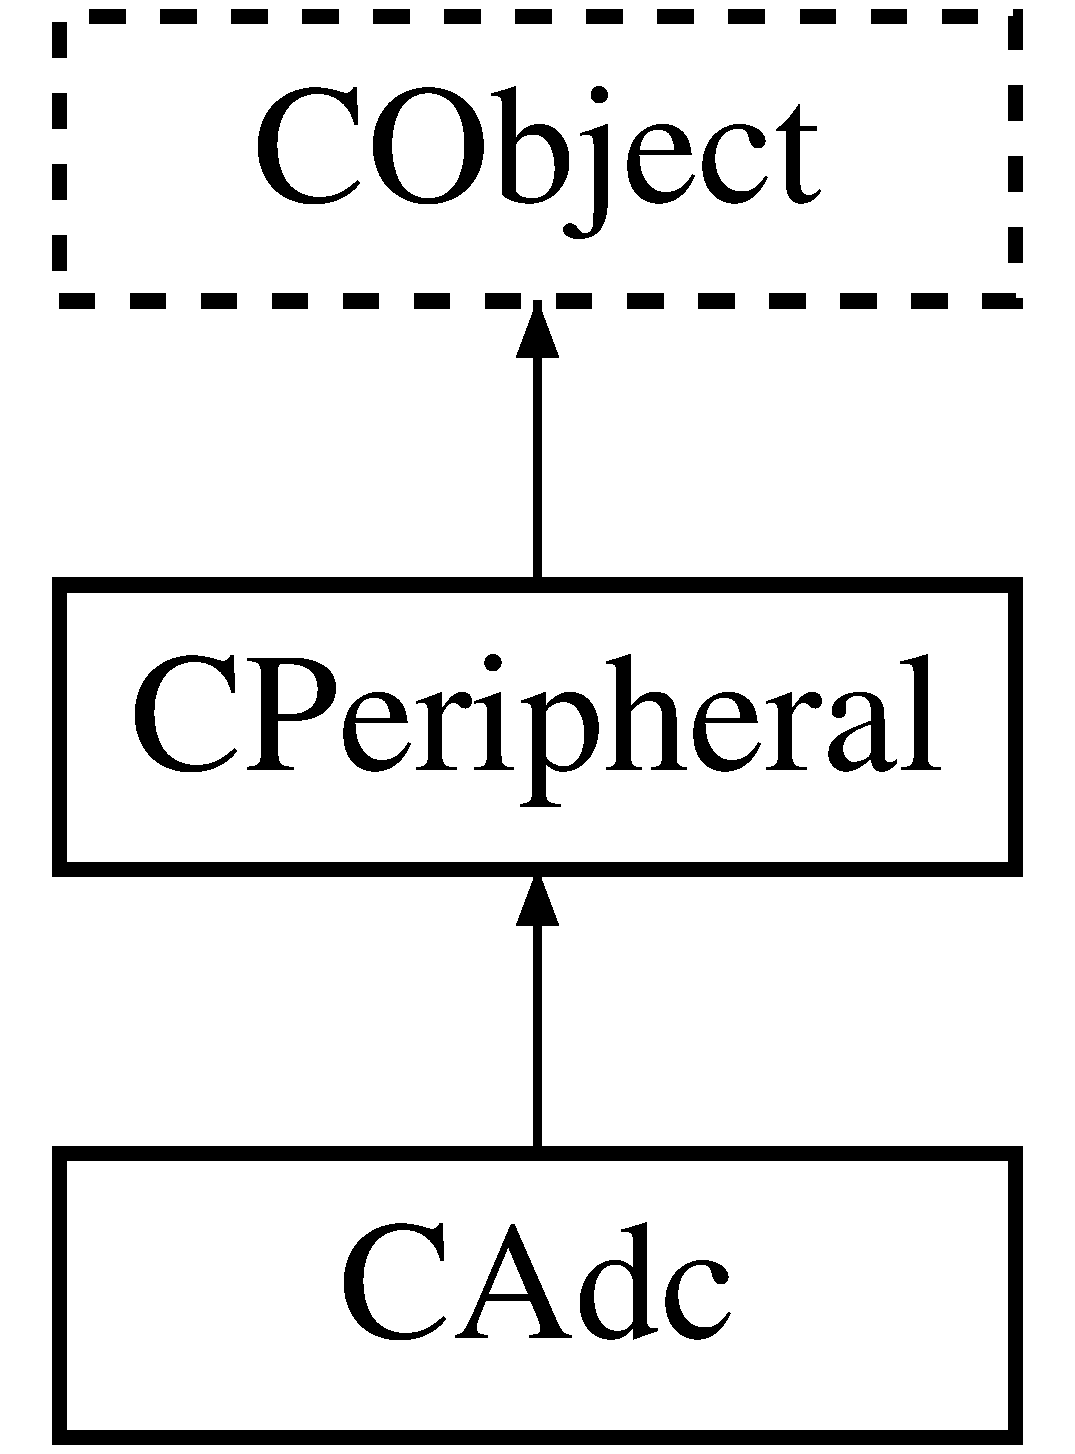
\includegraphics[height=3.000000cm]{class_c_adc}
\end{center}
\end{figure}
\subsection*{Public Member Functions}
\begin{DoxyCompactItemize}
\item 
\hyperlink{class_c_adc_a3d122c0e7fe686958371eabc9ed0db3f}{C\-Adc} (A\-D\-C\-\_\-\-C\-H\-\_\-\-T ch)
\item 
virtual void \hyperlink{class_c_adc_a11f59e83f9a3815e7980273a0b9bdd5b}{enable} (bool filtr=true)
\item 
virtual void \hyperlink{class_c_adc_ad3fc0560a6fbbca6d1cae12b187f98b7}{disable} ()
\item 
virtual int \hyperlink{class_c_adc_aa0748ed4e15aded89101060e388af8be}{read} ()
\item 
virtual int \hyperlink{class_c_adc_a20a6e83792c914309d2b0845e798b4d7}{read} (float filter, int count=3)
\item 
virtual int \hyperlink{class_c_adc_a31643f0558a614c013d476818156a1a1}{read} (int samples, \hyperlink{class_c_timer}{C\-Timer} \&interval)
\item 
virtual \hyperlink{class_c_adc_a678a8b70b4d4a2537c99eaba562e75b8}{operator float} ()
\item 
\hypertarget{class_c_adc_ad27b537dba363079fc68ee48050183d6}{void {\bfseries begin} ()}\label{class_c_adc_ad27b537dba363079fc68ee48050183d6}

\item 
\hypertarget{class_c_adc_a83103970c96cf7f0638bc44a11fa68b6}{void {\bfseries end} ()}\label{class_c_adc_a83103970c96cf7f0638bc44a11fa68b6}

\end{DoxyCompactItemize}


\subsection{Detailed Description}
an Analog-\/to-\/\-Digital converter class. 

\subsection{Constructor \& Destructor Documentation}
\hypertarget{class_c_adc_a3d122c0e7fe686958371eabc9ed0db3f}{\index{C\-Adc@{C\-Adc}!C\-Adc@{C\-Adc}}
\index{C\-Adc@{C\-Adc}!CAdc@{C\-Adc}}
\subsubsection[{C\-Adc}]{\setlength{\rightskip}{0pt plus 5cm}C\-Adc\-::\-C\-Adc (
\begin{DoxyParamCaption}
\item[{A\-D\-C\-\_\-\-C\-H\-\_\-\-T}]{ch}
\end{DoxyParamCaption}
)}}\label{class_c_adc_a3d122c0e7fe686958371eabc9ed0db3f}
Constructs a \hyperlink{class_c_adc}{C\-Adc} object with an A\-D pin. 
\begin{DoxyParams}{Parameters}
{\em ch} & is a A\-D\-C\-\_\-\-C\-H\-\_\-\-T to specified an A\-D pin to connected to the object.\\
\hline
\end{DoxyParams}

\begin{DoxyCode}
Example:
    \hyperlink{class_c_adc}{CAdc} ad(AD5);
    ad.begin();
\end{DoxyCode}
 

\subsection{Member Function Documentation}
\hypertarget{class_c_adc_ad3fc0560a6fbbca6d1cae12b187f98b7}{\index{C\-Adc@{C\-Adc}!disable@{disable}}
\index{disable@{disable}!CAdc@{C\-Adc}}
\subsubsection[{disable}]{\setlength{\rightskip}{0pt plus 5cm}virtual void C\-Adc\-::disable (
\begin{DoxyParamCaption}
{}
\end{DoxyParamCaption}
)\hspace{0.3cm}{\ttfamily [virtual]}}}\label{class_c_adc_ad3fc0560a6fbbca6d1cae12b187f98b7}
Disable the A\-D\-C function on the object \hypertarget{class_c_adc_a11f59e83f9a3815e7980273a0b9bdd5b}{\index{C\-Adc@{C\-Adc}!enable@{enable}}
\index{enable@{enable}!CAdc@{C\-Adc}}
\subsubsection[{enable}]{\setlength{\rightskip}{0pt plus 5cm}virtual void C\-Adc\-::enable (
\begin{DoxyParamCaption}
\item[{bool}]{filtr = {\ttfamily true}}
\end{DoxyParamCaption}
)\hspace{0.3cm}{\ttfamily [virtual]}}}\label{class_c_adc_a11f59e83f9a3815e7980273a0b9bdd5b}
Enable the A\-D\-C function on the object \hypertarget{class_c_adc_a678a8b70b4d4a2537c99eaba562e75b8}{\index{C\-Adc@{C\-Adc}!operator float@{operator float}}
\index{operator float@{operator float}!CAdc@{C\-Adc}}
\subsubsection[{operator float}]{\setlength{\rightskip}{0pt plus 5cm}virtual C\-Adc\-::operator float (
\begin{DoxyParamCaption}
{}
\end{DoxyParamCaption}
)\hspace{0.3cm}{\ttfamily [inline]}, {\ttfamily [virtual]}}}\label{class_c_adc_a678a8b70b4d4a2537c99eaba562e75b8}
A shorthand operator code to read A\-D\-C value \begin{DoxyReturn}{Returns}
a float value, divide by M\-A\-X\-\_\-\-A\-D\-C\-\_\-\-V\-A\-L\-U\-E
\end{DoxyReturn}

\begin{DoxyCode}
Example:
    \hyperlink{class_c_adc}{CAdc} ad(AD5);
    ad.begin();

    \textcolor{keywordtype}{float} value = ad;
\end{DoxyCode}
 \hypertarget{class_c_adc_aa0748ed4e15aded89101060e388af8be}{\index{C\-Adc@{C\-Adc}!read@{read}}
\index{read@{read}!CAdc@{C\-Adc}}
\subsubsection[{read}]{\setlength{\rightskip}{0pt plus 5cm}virtual int C\-Adc\-::read (
\begin{DoxyParamCaption}
{}
\end{DoxyParamCaption}
)\hspace{0.3cm}{\ttfamily [virtual]}}}\label{class_c_adc_aa0748ed4e15aded89101060e388af8be}
Read the A\-D\-C value from the A\-D pin \begin{DoxyReturn}{Returns}
10 bits resolution (0$\sim$1023) A\-D\-C value, if return -\/1, an overrun error. 
\end{DoxyReturn}
\hypertarget{class_c_adc_a20a6e83792c914309d2b0845e798b4d7}{\index{C\-Adc@{C\-Adc}!read@{read}}
\index{read@{read}!CAdc@{C\-Adc}}
\subsubsection[{read}]{\setlength{\rightskip}{0pt plus 5cm}virtual int C\-Adc\-::read (
\begin{DoxyParamCaption}
\item[{float}]{filter, }
\item[{int}]{count = {\ttfamily 3}}
\end{DoxyParamCaption}
)\hspace{0.3cm}{\ttfamily [virtual]}}}\label{class_c_adc_a20a6e83792c914309d2b0845e798b4d7}
Read the A\-D\-C value from the A\-D pin with Compare-\/\-Filter 
\begin{DoxyParams}[1]{Parameters}
\mbox{\tt in}  & {\em filter} & a float value to identify the offset range with last value. (0.\-1 = 10\%, 0.\-25=25\%) \\
\hline
\mbox{\tt in}  & {\em count} & a integer value to identify to retry count if A\-D\-C value over the filter range. (default value is 3) \\
\hline
\end{DoxyParams}
\begin{DoxyReturn}{Returns}
12 bits resolution (0$\sim$4095) A\-D\-C value
\end{DoxyReturn}

\begin{DoxyCode}
Example:
    \hyperlink{class_c_adc}{CAdc} ad(AD0);
    ad.begin();
    \textcolor{keywordtype}{int} value = ad.read(0.25, 3);   \textcolor{comment}{// if AD value over 25% with last value, try to read the AD value 3
       times.}
\end{DoxyCode}
 \hypertarget{class_c_adc_a31643f0558a614c013d476818156a1a1}{\index{C\-Adc@{C\-Adc}!read@{read}}
\index{read@{read}!CAdc@{C\-Adc}}
\subsubsection[{read}]{\setlength{\rightskip}{0pt plus 5cm}virtual int C\-Adc\-::read (
\begin{DoxyParamCaption}
\item[{int}]{samples, }
\item[{{\bf C\-Timer} \&}]{interval}
\end{DoxyParamCaption}
)\hspace{0.3cm}{\ttfamily [virtual]}}}\label{class_c_adc_a31643f0558a614c013d476818156a1a1}
Read the A\-D\-C value from the A\-D pin with Median-\/\-Filter 
\begin{DoxyParams}[1]{Parameters}
\mbox{\tt in}  & {\em samples} & a integer to identify how many A\-D\-C value read in sample buffer. \\
\hline
\mbox{\tt in}  & {\em interval} & a \hyperlink{class_c_timer}{C\-Timer} object to provide the interval timer service. \\
\hline
\end{DoxyParams}
\begin{DoxyReturn}{Returns}
12 bits resolution (0$\sim$4095) A\-D\-C value
\end{DoxyReturn}

\begin{DoxyCode}
Example:
        \hyperlink{class_c_adc}{CAdc} ad(AD0);
        ad.begin();

        CTime t(TIMER0);
        t.setting(10, 50);          \textcolor{comment}{// 10x50 = 500us interval}
        t.begin();

        \textcolor{keywordtype}{int} value = ad.read(5, t);  \textcolor{comment}{// ADC value with Median-Filter, total 5 samples, interval 500us}
\end{DoxyCode}
 \href{http://en.wikipedia.org/wiki/Median_filter}{\tt Wi\-Ki for Median Filter} 

The documentation for this class was generated from the following file\-:\begin{DoxyCompactItemize}
\item 
adc.\-h\end{DoxyCompactItemize}

\hypertarget{class_c_bus}{\section{C\-Bus Class Reference}
\label{class_c_bus}\index{C\-Bus@{C\-Bus}}
}


{\ttfamily \#include \char`\"{}class/bus.\-h\char`\"{}}

Inheritance diagram for C\-Bus\-:\begin{figure}[H]
\begin{center}
\leavevmode
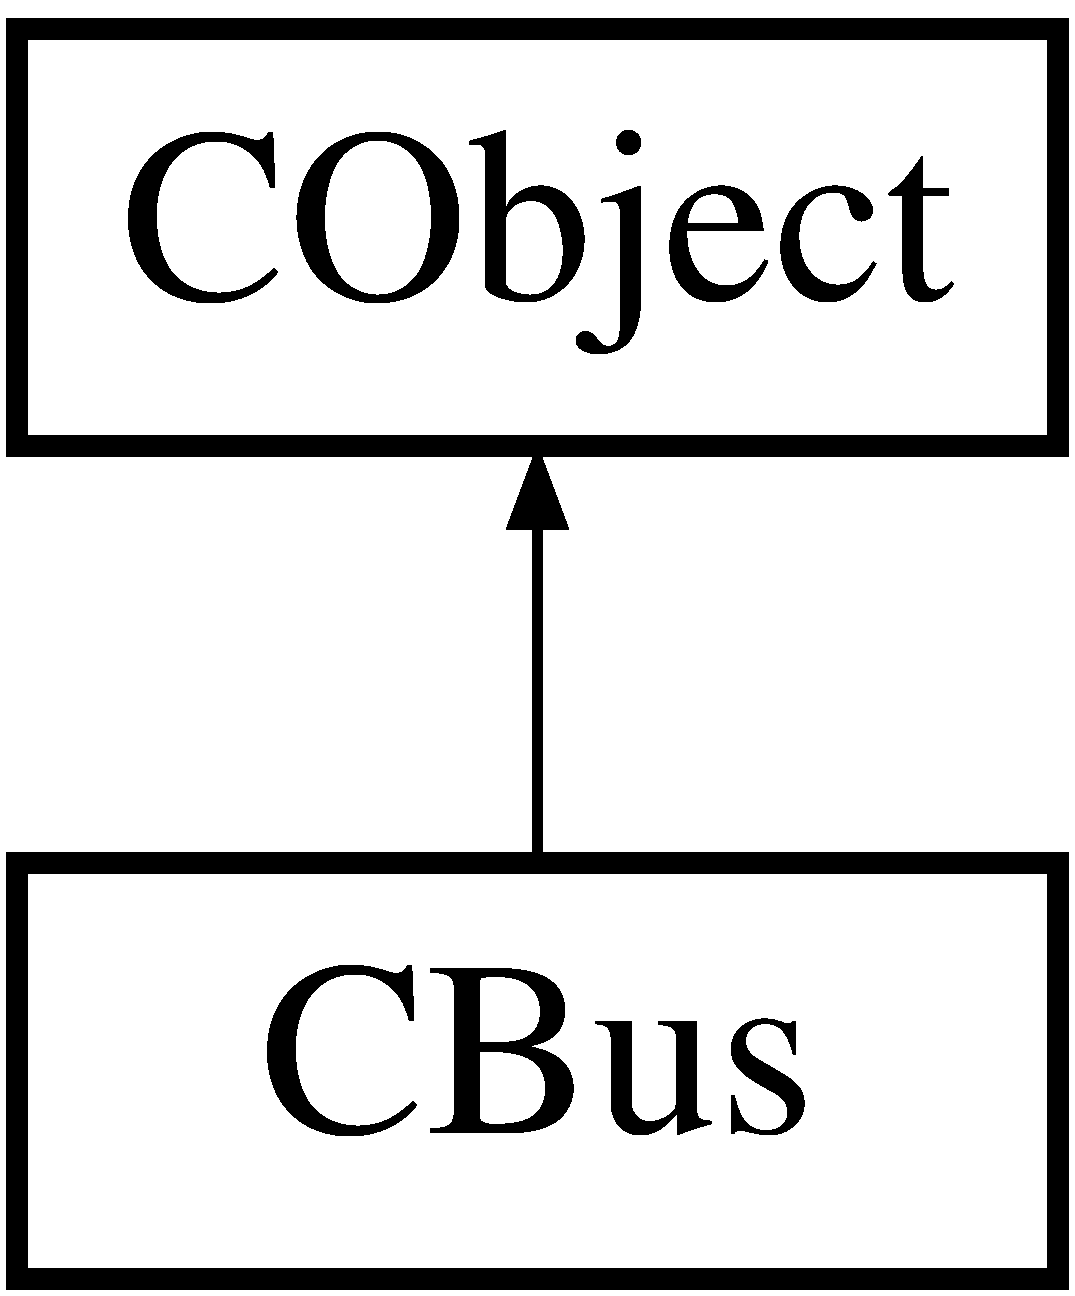
\includegraphics[height=3.000000cm]{de/d89/class_c_bus}
\end{center}
\end{figure}
\subsection*{Public Member Functions}
\begin{DoxyCompactItemize}
\item 
\hyperlink{class_c_bus_a5f859ac1582a6cbe9b5b420c6c051e63}{C\-Bus} (\hyperlink{group___enumerations_ga65a2241721e4acb573e0c3fe29ac432f}{P\-I\-N\-\_\-\-N\-A\-M\-E\-\_\-\-T} \hyperlink{class_c_bus_a94da38619defc1c41c16c04c4c7991f8}{pin},...)
\item 
void \hyperlink{class_c_bus_a5f797dca77eb5a86048c65e567a2d233}{output} ()
\item 
void \hyperlink{class_c_bus_ad45a06493f12aef3d096ac3ed86a3b8f}{input} (\hyperlink{group___enumerations_ga9f8f32709b482732d6e377ff26da36ef}{P\-I\-N\-\_\-\-I\-N\-P\-U\-T\-\_\-\-M\-O\-D\-E\-\_\-\-T} mode=\hyperlink{group___enumerations_gga9f8f32709b482732d6e377ff26da36efa781a7f23ae9b0dbdc6edfdcfd3be75df}{I\-N\-T\-E\-R\-N\-A\-L\-\_\-\-P\-U\-L\-L\-\_\-\-U\-P})
\item 
virtual void \hyperlink{class_c_bus_a4852669ff7ae53e68cf125aa49a87bd0}{write} (uint32\-\_\-t val)
\item 
virtual uint32\-\_\-t \hyperlink{class_c_bus_ae5c9d649c6f6b22a93fb29e0152a57c1}{read} ()
\item 
\hyperlink{class_c_pin}{C\-Pin} \& \hyperlink{class_c_bus_a94da38619defc1c41c16c04c4c7991f8}{pin} (int index)
\item 
\hyperlink{class_c_bus_add3835bd7327b63bdaa480938d5a8adc}{operator uint32\-\_\-t} ()
\item 
void \hyperlink{class_c_bus_a9f639b395906de4549c51deb0a0ad79c}{operator=} (uint32\-\_\-t val)
\item 
bool \hyperlink{class_c_bus_a55d1c493025b37e0f34801b8ced31068}{operator==} (uint32\-\_\-t val)
\item 
bool \hyperlink{class_c_bus_a3ea59ccbb16b92e2763a00b3baa10fd6}{operator!=} (uint32\-\_\-t val)
\item 
\hyperlink{class_c_pin}{C\-Pin} \& \hyperlink{class_c_bus_a12e4d076164971de589cbc5b2f6537e2}{operator\mbox{[}$\,$\mbox{]}} (int index)
\item 
int \hyperlink{class_c_bus_a4fa0e4c537c237278fe8092f4d8e26fb}{count} ()
\end{DoxyCompactItemize}


\subsection{Detailed Description}
A digital input/output bus, used for reading/writing the state of a collection of pins. 

\subsection{Constructor \& Destructor Documentation}
\hypertarget{class_c_bus_a5f859ac1582a6cbe9b5b420c6c051e63}{\index{C\-Bus@{C\-Bus}!C\-Bus@{C\-Bus}}
\index{C\-Bus@{C\-Bus}!CBus@{C\-Bus}}
\subsubsection[{C\-Bus}]{\setlength{\rightskip}{0pt plus 5cm}C\-Bus\-::\-C\-Bus (
\begin{DoxyParamCaption}
\item[{{\bf P\-I\-N\-\_\-\-N\-A\-M\-E\-\_\-\-T}}]{pin, }
\item[{}]{...}
\end{DoxyParamCaption}
)}}\label{class_c_bus_a5f859ac1582a6cbe9b5b420c6c051e63}
Constructs a \hyperlink{class_c_bus}{C\-Bus} object to connect to the specified pins. 
\begin{DoxyParams}{Parameters}
{\em pin} & ... are P\-I\-N\-\_\-\-N\-A\-M\-E\-\_\-\-T to specified one or more pins to the \hyperlink{class_c_bus}{C\-Bus}.\\
\hline
\end{DoxyParams}

\begin{DoxyCode}
Example:
        \hyperlink{class_c_bus}{CBus} bus(\hyperlink{group___enumerations_gga65a2241721e4acb573e0c3fe29ac432fa19b235491a16a3e7f91872f46a33a4a6}{P21}, \hyperlink{group___enumerations_gga65a2241721e4acb573e0c3fe29ac432fa7010befcbd538e2d53cf35755cbc4663}{P22}, \hyperlink{group___enumerations_gga65a2241721e4acb573e0c3fe29ac432fac7bf4234043357a0b854b3818a8d33e6}{P23}, \hyperlink{group___enumerations_gga65a2241721e4acb573e0c3fe29ac432fa98300b37c344c1c3e73a3f9ddb160bab}{P24}, \hyperlink{group___enumerations_gga65a2241721e4acb573e0c3fe29ac432fadc6f24fd6915a3f2786a1b7045406924}{END});  \textcolor{comment}{// Collect P21~P24 in the CBus object.}
        bus.output();                       \textcolor{comment}{// Set the bus as output pins.}
\end{DoxyCode}
 \begin{DoxyRemark}{Remarks}
to 'E\-N\-D' of the pin arguments is M\-U\-S\-T!! 
\end{DoxyRemark}


\subsection{Member Function Documentation}
\hypertarget{class_c_bus_a5f797dca77eb5a86048c65e567a2d233}{\index{C\-Bus@{C\-Bus}!output@{output}}
\index{output@{output}!CBus@{C\-Bus}}
\subsubsection[{output}]{\setlength{\rightskip}{0pt plus 5cm}void C\-Bus\-::output (
\begin{DoxyParamCaption}
{}
\end{DoxyParamCaption}
)}}\label{class_c_bus_a5f797dca77eb5a86048c65e567a2d233}
Call the member function to set the bus as output pins. 
\begin{DoxyParams}{Parameters}
{\em mode} & is a P\-I\-N\-\_\-\-O\-U\-T\-P\-U\-T\-\_\-\-M\-O\-D\-E\-\_\-\-T, default is O\-P\-E\-N\-\_\-\-D\-R\-A\-I\-N (provide current). \\
\hline
\end{DoxyParams}
\hypertarget{class_c_bus_ad45a06493f12aef3d096ac3ed86a3b8f}{\index{C\-Bus@{C\-Bus}!input@{input}}
\index{input@{input}!CBus@{C\-Bus}}
\subsubsection[{input}]{\setlength{\rightskip}{0pt plus 5cm}void C\-Bus\-::input (
\begin{DoxyParamCaption}
\item[{{\bf P\-I\-N\-\_\-\-I\-N\-P\-U\-T\-\_\-\-M\-O\-D\-E\-\_\-\-T}}]{mode = {\ttfamily {\bf I\-N\-T\-E\-R\-N\-A\-L\-\_\-\-P\-U\-L\-L\-\_\-\-U\-P}}}
\end{DoxyParamCaption}
)}}\label{class_c_bus_ad45a06493f12aef3d096ac3ed86a3b8f}
Call the member function to set the bus as input pins 
\begin{DoxyParams}{Parameters}
{\em mode} & is a P\-I\-N\-\_\-\-I\-N\-P\-U\-T\-\_\-\-M\-O\-D\-E\-\_\-\-T, default is I\-N\-T\-E\-R\-N\-A\-L\-\_\-\-P\-U\-T\-T\-\_\-\-U\-P. \\
\hline
\end{DoxyParams}
\hypertarget{class_c_bus_a4852669ff7ae53e68cf125aa49a87bd0}{\index{C\-Bus@{C\-Bus}!write@{write}}
\index{write@{write}!CBus@{C\-Bus}}
\subsubsection[{write}]{\setlength{\rightskip}{0pt plus 5cm}virtual void C\-Bus\-::write (
\begin{DoxyParamCaption}
\item[{uint32\-\_\-t}]{val}
\end{DoxyParamCaption}
)\hspace{0.3cm}{\ttfamily [virtual]}}}\label{class_c_bus_a4852669ff7ae53e68cf125aa49a87bd0}
Call the member function to write a value to the bus. 
\begin{DoxyParams}{Parameters}
{\em val} & is a unsigned integer to map the bit wide value to pins. \\
\hline
\end{DoxyParams}
\hypertarget{class_c_bus_ae5c9d649c6f6b22a93fb29e0152a57c1}{\index{C\-Bus@{C\-Bus}!read@{read}}
\index{read@{read}!CBus@{C\-Bus}}
\subsubsection[{read}]{\setlength{\rightskip}{0pt plus 5cm}virtual uint32\-\_\-t C\-Bus\-::read (
\begin{DoxyParamCaption}
{}
\end{DoxyParamCaption}
)\hspace{0.3cm}{\ttfamily [virtual]}}}\label{class_c_bus_ae5c9d649c6f6b22a93fb29e0152a57c1}
Call the member function to retrieve a value from pins. \begin{DoxyReturn}{Returns}
a unsigned integer value that map the bit-\/wide of pins. 
\end{DoxyReturn}
\hypertarget{class_c_bus_a94da38619defc1c41c16c04c4c7991f8}{\index{C\-Bus@{C\-Bus}!pin@{pin}}
\index{pin@{pin}!CBus@{C\-Bus}}
\subsubsection[{pin}]{\setlength{\rightskip}{0pt plus 5cm}{\bf C\-Pin}\& C\-Bus\-::pin (
\begin{DoxyParamCaption}
\item[{int}]{index}
\end{DoxyParamCaption}
)}}\label{class_c_bus_a94da38619defc1c41c16c04c4c7991f8}
Call the member function to retrieve a identity pin from bus. \begin{DoxyReturn}{Returns}
\hyperlink{class_c_pin}{C\-Pin} 
\end{DoxyReturn}
\hypertarget{class_c_bus_add3835bd7327b63bdaa480938d5a8adc}{\index{C\-Bus@{C\-Bus}!operator uint32\-\_\-t@{operator uint32\-\_\-t}}
\index{operator uint32\-\_\-t@{operator uint32\-\_\-t}!CBus@{C\-Bus}}
\subsubsection[{operator uint32\-\_\-t}]{\setlength{\rightskip}{0pt plus 5cm}C\-Bus\-::operator uint32\-\_\-t (
\begin{DoxyParamCaption}
{}
\end{DoxyParamCaption}
)\hspace{0.3cm}{\ttfamily [inline]}}}\label{class_c_bus_add3835bd7327b63bdaa480938d5a8adc}
A shorthand for read


\begin{DoxyCode}
Example:
        \hyperlink{class_c_bus}{CBus} bus(\hyperlink{group___enumerations_gga65a2241721e4acb573e0c3fe29ac432fa19b235491a16a3e7f91872f46a33a4a6}{P21}, \hyperlink{group___enumerations_gga65a2241721e4acb573e0c3fe29ac432fa7010befcbd538e2d53cf35755cbc4663}{P22}, \hyperlink{group___enumerations_gga65a2241721e4acb573e0c3fe29ac432fac7bf4234043357a0b854b3818a8d33e6}{P23}, \hyperlink{group___enumerations_gga65a2241721e4acb573e0c3fe29ac432fa98300b37c344c1c3e73a3f9ddb160bab}{P24}, \hyperlink{group___enumerations_gga65a2241721e4acb573e0c3fe29ac432fadc6f24fd6915a3f2786a1b7045406924}{END});  \textcolor{comment}{// Collect P21~P24 in the CBus object.}
        bus.input();                        \textcolor{comment}{// Set the bus as input pins.}
        uint32\_t val = bus;                 \textcolor{comment}{// Read a value from bus.}
\end{DoxyCode}
 \hypertarget{class_c_bus_a9f639b395906de4549c51deb0a0ad79c}{\index{C\-Bus@{C\-Bus}!operator=@{operator=}}
\index{operator=@{operator=}!CBus@{C\-Bus}}
\subsubsection[{operator=}]{\setlength{\rightskip}{0pt plus 5cm}void C\-Bus\-::operator= (
\begin{DoxyParamCaption}
\item[{uint32\-\_\-t}]{val}
\end{DoxyParamCaption}
)\hspace{0.3cm}{\ttfamily [inline]}}}\label{class_c_bus_a9f639b395906de4549c51deb0a0ad79c}
A shorthand for write


\begin{DoxyCode}
Example:
        \hyperlink{class_c_bus}{CBus} bus(\hyperlink{group___enumerations_gga65a2241721e4acb573e0c3fe29ac432fa19b235491a16a3e7f91872f46a33a4a6}{P21}, \hyperlink{group___enumerations_gga65a2241721e4acb573e0c3fe29ac432fa7010befcbd538e2d53cf35755cbc4663}{P22}, \hyperlink{group___enumerations_gga65a2241721e4acb573e0c3fe29ac432fac7bf4234043357a0b854b3818a8d33e6}{P23}, \hyperlink{group___enumerations_gga65a2241721e4acb573e0c3fe29ac432fa98300b37c344c1c3e73a3f9ddb160bab}{P24}, \hyperlink{group___enumerations_gga65a2241721e4acb573e0c3fe29ac432fadc6f24fd6915a3f2786a1b7045406924}{END});  \textcolor{comment}{// Collect P21~P24 in the CBus object.}
        bus.output();                       \textcolor{comment}{// Set the bus as output pins.}
        bus = 0x05;                         \textcolor{comment}{// Write 0x05 to bus.}
\end{DoxyCode}
 \hypertarget{class_c_bus_a55d1c493025b37e0f34801b8ced31068}{\index{C\-Bus@{C\-Bus}!operator==@{operator==}}
\index{operator==@{operator==}!CBus@{C\-Bus}}
\subsubsection[{operator==}]{\setlength{\rightskip}{0pt plus 5cm}bool C\-Bus\-::operator== (
\begin{DoxyParamCaption}
\item[{uint32\-\_\-t}]{val}
\end{DoxyParamCaption}
)\hspace{0.3cm}{\ttfamily [inline]}}}\label{class_c_bus_a55d1c493025b37e0f34801b8ced31068}
A shorthand for equal to... \begin{DoxyReturn}{Returns}
true if the bus==val, otherwise, failed. 
\end{DoxyReturn}
\hypertarget{class_c_bus_a3ea59ccbb16b92e2763a00b3baa10fd6}{\index{C\-Bus@{C\-Bus}!operator!=@{operator!=}}
\index{operator!=@{operator!=}!CBus@{C\-Bus}}
\subsubsection[{operator!=}]{\setlength{\rightskip}{0pt plus 5cm}bool C\-Bus\-::operator!= (
\begin{DoxyParamCaption}
\item[{uint32\-\_\-t}]{val}
\end{DoxyParamCaption}
)\hspace{0.3cm}{\ttfamily [inline]}}}\label{class_c_bus_a3ea59ccbb16b92e2763a00b3baa10fd6}
A shorthand for not equal to... \begin{DoxyReturn}{Returns}
true if the bus not equal the val; otherwise, failed. 
\end{DoxyReturn}
\hypertarget{class_c_bus_a12e4d076164971de589cbc5b2f6537e2}{\index{C\-Bus@{C\-Bus}!operator\mbox{[}$\,$\mbox{]}@{operator[]}}
\index{operator\mbox{[}$\,$\mbox{]}@{operator[]}!CBus@{C\-Bus}}
\subsubsection[{operator[]}]{\setlength{\rightskip}{0pt plus 5cm}{\bf C\-Pin}\& C\-Bus\-::operator\mbox{[}$\,$\mbox{]} (
\begin{DoxyParamCaption}
\item[{int}]{index}
\end{DoxyParamCaption}
)\hspace{0.3cm}{\ttfamily [inline]}}}\label{class_c_bus_a12e4d076164971de589cbc5b2f6537e2}
A shorthand for array \begin{DoxyReturn}{Returns}
\hyperlink{class_c_pin}{C\-Pin}
\end{DoxyReturn}

\begin{DoxyCode}
Example:
        \hyperlink{class_c_bus}{CBus} bus(\hyperlink{group___enumerations_gga65a2241721e4acb573e0c3fe29ac432fa19b235491a16a3e7f91872f46a33a4a6}{P21}, \hyperlink{group___enumerations_gga65a2241721e4acb573e0c3fe29ac432fa7010befcbd538e2d53cf35755cbc4663}{P22}, \hyperlink{group___enumerations_gga65a2241721e4acb573e0c3fe29ac432fac7bf4234043357a0b854b3818a8d33e6}{P23}, \hyperlink{group___enumerations_gga65a2241721e4acb573e0c3fe29ac432fa98300b37c344c1c3e73a3f9ddb160bab}{P24}, \hyperlink{group___enumerations_gga65a2241721e4acb573e0c3fe29ac432fadc6f24fd6915a3f2786a1b7045406924}{END});  \textcolor{comment}{// Collect P21~P24 in the CBus object.}
        bus.output();                       \textcolor{comment}{// Set the bus as output pins.}
    bus[2] = \hyperlink{group___enumerations_gga6f24594071a026b31238ab8cb80d6a80a6a226f4143ca3b18999551694cdb72a8}{LOW};                       \textcolor{comment}{// Set P23 is LOW.}
\end{DoxyCode}
 \hypertarget{class_c_bus_a4fa0e4c537c237278fe8092f4d8e26fb}{\index{C\-Bus@{C\-Bus}!count@{count}}
\index{count@{count}!CBus@{C\-Bus}}
\subsubsection[{count}]{\setlength{\rightskip}{0pt plus 5cm}int C\-Bus\-::count (
\begin{DoxyParamCaption}
{}
\end{DoxyParamCaption}
)\hspace{0.3cm}{\ttfamily [inline]}}}\label{class_c_bus_a4fa0e4c537c237278fe8092f4d8e26fb}
Call the member function to retrieve the number of pins in the bus. \begin{DoxyReturn}{Returns}
integer value. 
\end{DoxyReturn}


The documentation for this class was generated from the following file\-:\begin{DoxyCompactItemize}
\item 
bus.\-h\end{DoxyCompactItemize}

\hypertarget{class_c_debug}{\section{C\-Debug Class Reference}
\label{class_c_debug}\index{C\-Debug@{C\-Debug}}
}


{\ttfamily \#include $<$debug.\-h$>$}

Inheritance diagram for C\-Debug\-:\begin{figure}[H]
\begin{center}
\leavevmode
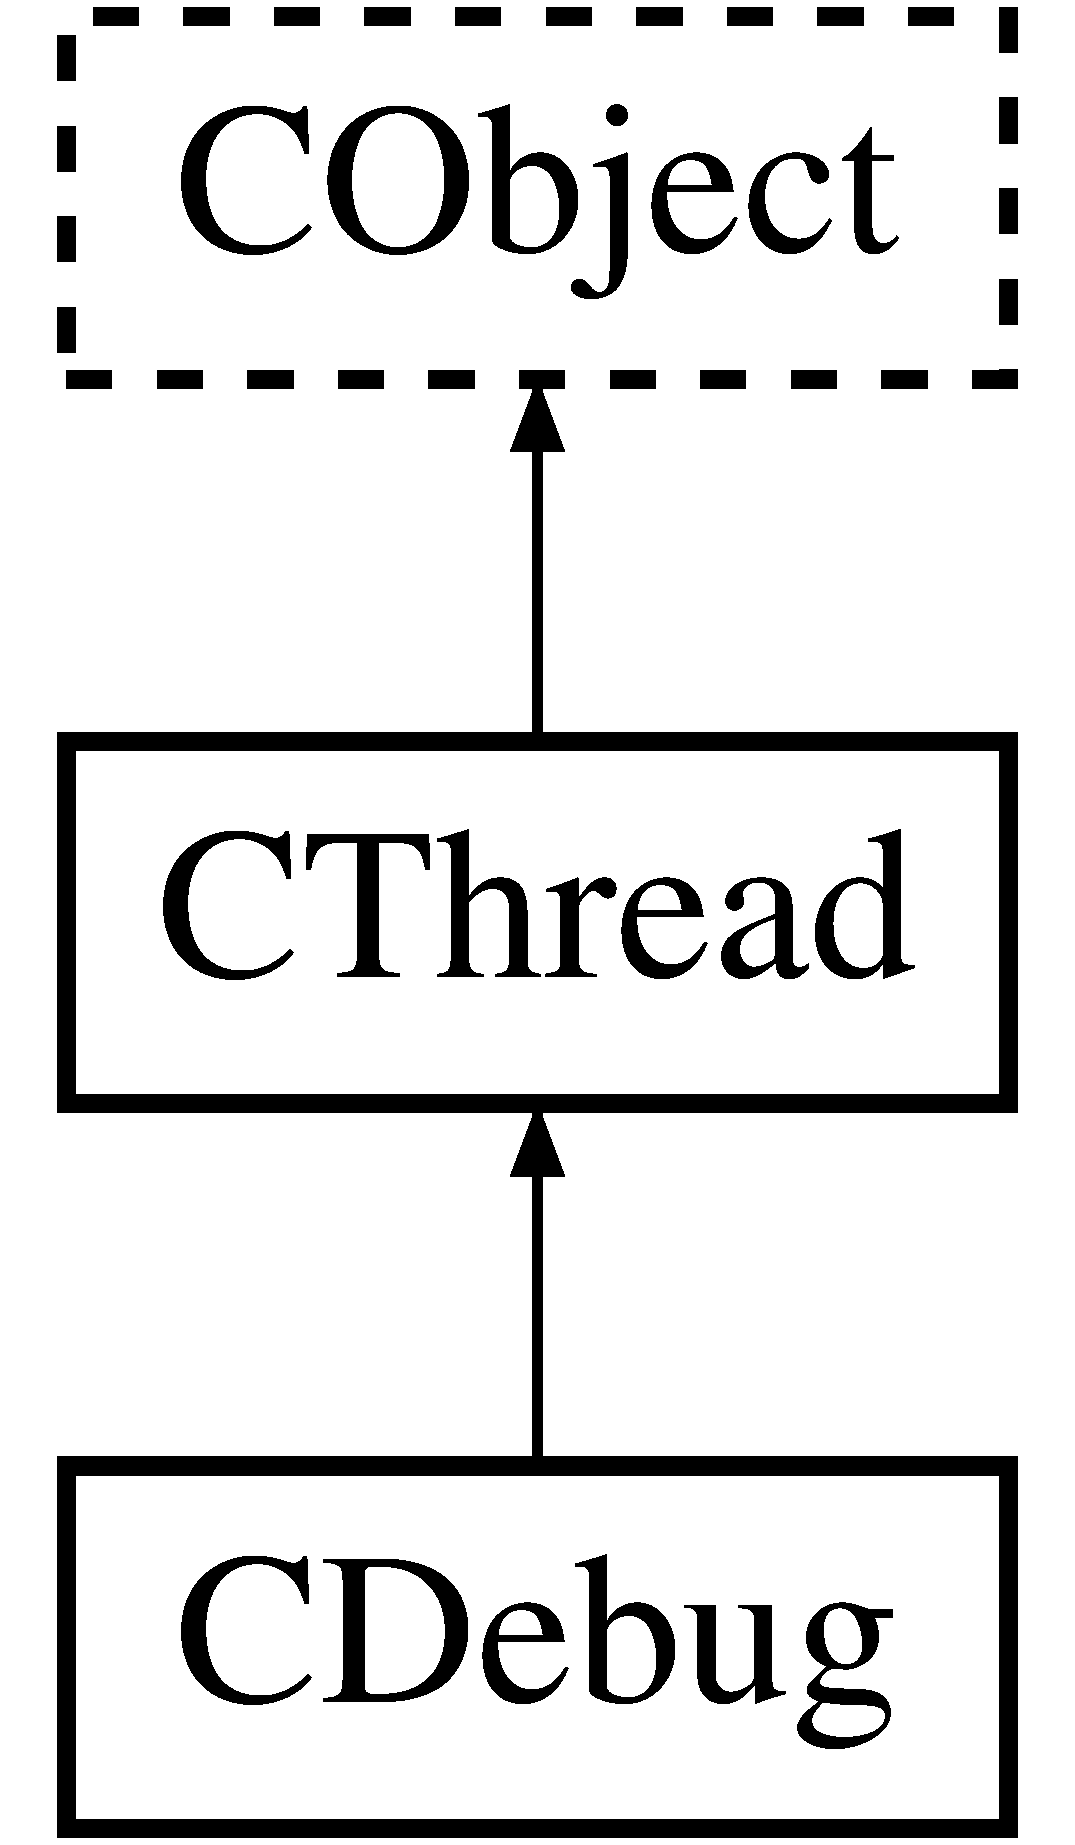
\includegraphics[height=3.000000cm]{d4/d37/class_c_debug}
\end{center}
\end{figure}
\subsection*{Public Member Functions}
\begin{DoxyCompactItemize}
\item 
\hyperlink{class_c_debug_a5e5390068e9a979029fc6df202ad8b6e}{C\-Debug} (\hyperlink{class_c_stream}{C\-Stream} \&s)
\item 
virtual bool \hyperlink{class_c_debug_a40d1b7f50b76311b3a7fb148e5b7e2ea}{start} ()
\item 
virtual void \hyperlink{class_c_debug_a525c9b7e5f56eca7017ee8a519f86a3e}{wait\-To\-Debug\-Mode} ()
\item 
virtual void \hyperlink{class_c_debug_a89c983c24d2a2934187d25a27f6c1aa9}{printf} (L\-P\-C\-T\-S\-T\-R format, va\-\_\-list varg)
\item 
virtual void \hyperlink{class_c_debug_a4f55fe7d7a21e9386da0484a1e4cd4cd}{printf} (L\-P\-C\-T\-S\-T\-R format,...)
\item 
virtual void \hyperlink{class_c_debug_a69b3be339e7fe9c991b39ef0f0e452c6}{println} (L\-P\-C\-T\-S\-T\-R format,...)
\item 
virtual void \hyperlink{class_c_debug_a6e7fadf6162782fa5b83635b737fb880}{println} (int value)
\item 
virtual void \hyperlink{class_c_debug_aa58d1c7c44e669a77bd8fdf3e58d68cd}{println} (uint32\-\_\-t value)
\item 
virtual void \hyperlink{class_c_debug_ac129190a73c1ce50df847d61c57641c4}{println} (float value)
\item 
virtual int \hyperlink{class_c_debug_a260233f4b1d98901555a249c3f7ad7be}{breakpoint} (L\-P\-C\-T\-S\-T\-R desc=N\-U\-L\-L)
\item 
virtual void \hyperlink{class_c_debug_ae83e3ecc41e21c19d2cfbea15459a7c9}{println} (\hyperlink{class_c_string}{C\-String} \&str)
\item 
virtual bool \hyperlink{class_c_debug_ab90cf9f4b16af5e740ac6a503f612224}{is\-Debug\-Mode} ()
\item 
virtual int \hyperlink{class_c_debug_ad4b4b7f29bf53500532e00aabb62deab}{is\-Any\-Key} ()
\item 
virtual void \hyperlink{class_c_debug_a8135b97d1fbae13f5a4952e3bbf50d34}{putc} (int c)
\item 
int \hyperlink{class_c_debug_a3c07626045ffa3227794e7cc080f5e36}{bp} ()
\item 
\hyperlink{class_c_debug_a5a1359725fca8337c5967a3c1811c460}{operator bool} ()
\end{DoxyCompactItemize}
\subsection*{Protected Member Functions}
\begin{DoxyCompactItemize}
\item 
virtual void \hyperlink{class_c_debug_a9a3e40cc8ee5d0c2a41577f658779c71}{run} ()
\end{DoxyCompactItemize}
\subsection*{Protected Attributes}
\begin{DoxyCompactItemize}
\item 
\hyperlink{class_c_stream}{C\-Stream} $\ast$ \hyperlink{class_c_debug_ab0e3c0c44f27c27a9fafa30866854cbe}{m\-\_\-stream}
\item 
\hyperlink{class_c_shell}{C\-Shell} \hyperlink{class_c_debug_a1e4ada8bb77d3cbcfaf614f0a657d6c7}{m\-\_\-shell}
\item 
\hyperlink{class_c_mutex}{C\-Mutex} \hyperlink{class_c_debug_a5c8a50a383cc0f5ddd26efb72d6b4794}{m\-\_\-mutex}
\end{DoxyCompactItemize}
\subsection*{Additional Inherited Members}


\subsection{Constructor \& Destructor Documentation}
\hypertarget{class_c_debug_a5e5390068e9a979029fc6df202ad8b6e}{\index{C\-Debug@{C\-Debug}!C\-Debug@{C\-Debug}}
\index{C\-Debug@{C\-Debug}!CDebug@{C\-Debug}}
\subsubsection[{C\-Debug}]{\setlength{\rightskip}{0pt plus 5cm}C\-Debug\-::\-C\-Debug (
\begin{DoxyParamCaption}
\item[{{\bf C\-Stream} \&}]{s}
\end{DoxyParamCaption}
)}}\label{class_c_debug_a5e5390068e9a979029fc6df202ad8b6e}


\subsection{Member Function Documentation}
\hypertarget{class_c_debug_a40d1b7f50b76311b3a7fb148e5b7e2ea}{\index{C\-Debug@{C\-Debug}!start@{start}}
\index{start@{start}!CDebug@{C\-Debug}}
\subsubsection[{start}]{\setlength{\rightskip}{0pt plus 5cm}virtual bool C\-Debug\-::start (
\begin{DoxyParamCaption}
{}
\end{DoxyParamCaption}
)\hspace{0.3cm}{\ttfamily [virtual]}}}\label{class_c_debug_a40d1b7f50b76311b3a7fb148e5b7e2ea}
Call the member function to start the thread. \begin{DoxyNote}{Note}
the \hyperlink{class_c_debug_a40d1b7f50b76311b3a7fb148e5b7e2ea}{start()} is an overload member function of \hyperlink{class_c_thread}{C\-Thread}. 
\end{DoxyNote}


Reimplemented from \hyperlink{class_c_thread_aacf955d1852e74da1f989251955ee6ec}{C\-Thread}.

\hypertarget{class_c_debug_a525c9b7e5f56eca7017ee8a519f86a3e}{\index{C\-Debug@{C\-Debug}!wait\-To\-Debug\-Mode@{wait\-To\-Debug\-Mode}}
\index{wait\-To\-Debug\-Mode@{wait\-To\-Debug\-Mode}!CDebug@{C\-Debug}}
\subsubsection[{wait\-To\-Debug\-Mode}]{\setlength{\rightskip}{0pt plus 5cm}virtual void C\-Debug\-::wait\-To\-Debug\-Mode (
\begin{DoxyParamCaption}
{}
\end{DoxyParamCaption}
)\hspace{0.3cm}{\ttfamily [virtual]}}}\label{class_c_debug_a525c9b7e5f56eca7017ee8a519f86a3e}
\hypertarget{class_c_debug_a89c983c24d2a2934187d25a27f6c1aa9}{\index{C\-Debug@{C\-Debug}!printf@{printf}}
\index{printf@{printf}!CDebug@{C\-Debug}}
\subsubsection[{printf}]{\setlength{\rightskip}{0pt plus 5cm}virtual void C\-Debug\-::printf (
\begin{DoxyParamCaption}
\item[{L\-P\-C\-T\-S\-T\-R}]{format, }
\item[{va\-\_\-list}]{varg}
\end{DoxyParamCaption}
)\hspace{0.3cm}{\ttfamily [virtual]}}}\label{class_c_debug_a89c983c24d2a2934187d25a27f6c1aa9}
\hypertarget{class_c_debug_a4f55fe7d7a21e9386da0484a1e4cd4cd}{\index{C\-Debug@{C\-Debug}!printf@{printf}}
\index{printf@{printf}!CDebug@{C\-Debug}}
\subsubsection[{printf}]{\setlength{\rightskip}{0pt plus 5cm}virtual void C\-Debug\-::printf (
\begin{DoxyParamCaption}
\item[{L\-P\-C\-T\-S\-T\-R}]{format, }
\item[{}]{...}
\end{DoxyParamCaption}
)\hspace{0.3cm}{\ttfamily [virtual]}}}\label{class_c_debug_a4f55fe7d7a21e9386da0484a1e4cd4cd}
\hypertarget{class_c_debug_a69b3be339e7fe9c991b39ef0f0e452c6}{\index{C\-Debug@{C\-Debug}!println@{println}}
\index{println@{println}!CDebug@{C\-Debug}}
\subsubsection[{println}]{\setlength{\rightskip}{0pt plus 5cm}virtual void C\-Debug\-::println (
\begin{DoxyParamCaption}
\item[{L\-P\-C\-T\-S\-T\-R}]{format, }
\item[{}]{...}
\end{DoxyParamCaption}
)\hspace{0.3cm}{\ttfamily [virtual]}}}\label{class_c_debug_a69b3be339e7fe9c991b39ef0f0e452c6}
\hypertarget{class_c_debug_a6e7fadf6162782fa5b83635b737fb880}{\index{C\-Debug@{C\-Debug}!println@{println}}
\index{println@{println}!CDebug@{C\-Debug}}
\subsubsection[{println}]{\setlength{\rightskip}{0pt plus 5cm}virtual void C\-Debug\-::println (
\begin{DoxyParamCaption}
\item[{int}]{value}
\end{DoxyParamCaption}
)\hspace{0.3cm}{\ttfamily [virtual]}}}\label{class_c_debug_a6e7fadf6162782fa5b83635b737fb880}
\hypertarget{class_c_debug_aa58d1c7c44e669a77bd8fdf3e58d68cd}{\index{C\-Debug@{C\-Debug}!println@{println}}
\index{println@{println}!CDebug@{C\-Debug}}
\subsubsection[{println}]{\setlength{\rightskip}{0pt plus 5cm}virtual void C\-Debug\-::println (
\begin{DoxyParamCaption}
\item[{uint32\-\_\-t}]{value}
\end{DoxyParamCaption}
)\hspace{0.3cm}{\ttfamily [virtual]}}}\label{class_c_debug_aa58d1c7c44e669a77bd8fdf3e58d68cd}
\hypertarget{class_c_debug_ac129190a73c1ce50df847d61c57641c4}{\index{C\-Debug@{C\-Debug}!println@{println}}
\index{println@{println}!CDebug@{C\-Debug}}
\subsubsection[{println}]{\setlength{\rightskip}{0pt plus 5cm}virtual void C\-Debug\-::println (
\begin{DoxyParamCaption}
\item[{float}]{value}
\end{DoxyParamCaption}
)\hspace{0.3cm}{\ttfamily [virtual]}}}\label{class_c_debug_ac129190a73c1ce50df847d61c57641c4}
\hypertarget{class_c_debug_a260233f4b1d98901555a249c3f7ad7be}{\index{C\-Debug@{C\-Debug}!breakpoint@{breakpoint}}
\index{breakpoint@{breakpoint}!CDebug@{C\-Debug}}
\subsubsection[{breakpoint}]{\setlength{\rightskip}{0pt plus 5cm}virtual int C\-Debug\-::breakpoint (
\begin{DoxyParamCaption}
\item[{L\-P\-C\-T\-S\-T\-R}]{desc = {\ttfamily NULL}}
\end{DoxyParamCaption}
)\hspace{0.3cm}{\ttfamily [virtual]}}}\label{class_c_debug_a260233f4b1d98901555a249c3f7ad7be}
\hypertarget{class_c_debug_ae83e3ecc41e21c19d2cfbea15459a7c9}{\index{C\-Debug@{C\-Debug}!println@{println}}
\index{println@{println}!CDebug@{C\-Debug}}
\subsubsection[{println}]{\setlength{\rightskip}{0pt plus 5cm}virtual void C\-Debug\-::println (
\begin{DoxyParamCaption}
\item[{{\bf C\-String} \&}]{str}
\end{DoxyParamCaption}
)\hspace{0.3cm}{\ttfamily [inline]}, {\ttfamily [virtual]}}}\label{class_c_debug_ae83e3ecc41e21c19d2cfbea15459a7c9}
\hypertarget{class_c_debug_ab90cf9f4b16af5e740ac6a503f612224}{\index{C\-Debug@{C\-Debug}!is\-Debug\-Mode@{is\-Debug\-Mode}}
\index{is\-Debug\-Mode@{is\-Debug\-Mode}!CDebug@{C\-Debug}}
\subsubsection[{is\-Debug\-Mode}]{\setlength{\rightskip}{0pt plus 5cm}virtual bool C\-Debug\-::is\-Debug\-Mode (
\begin{DoxyParamCaption}
{}
\end{DoxyParamCaption}
)\hspace{0.3cm}{\ttfamily [inline]}, {\ttfamily [virtual]}}}\label{class_c_debug_ab90cf9f4b16af5e740ac6a503f612224}
\hypertarget{class_c_debug_ad4b4b7f29bf53500532e00aabb62deab}{\index{C\-Debug@{C\-Debug}!is\-Any\-Key@{is\-Any\-Key}}
\index{is\-Any\-Key@{is\-Any\-Key}!CDebug@{C\-Debug}}
\subsubsection[{is\-Any\-Key}]{\setlength{\rightskip}{0pt plus 5cm}virtual int C\-Debug\-::is\-Any\-Key (
\begin{DoxyParamCaption}
{}
\end{DoxyParamCaption}
)\hspace{0.3cm}{\ttfamily [inline]}, {\ttfamily [virtual]}}}\label{class_c_debug_ad4b4b7f29bf53500532e00aabb62deab}
\hypertarget{class_c_debug_a8135b97d1fbae13f5a4952e3bbf50d34}{\index{C\-Debug@{C\-Debug}!putc@{putc}}
\index{putc@{putc}!CDebug@{C\-Debug}}
\subsubsection[{putc}]{\setlength{\rightskip}{0pt plus 5cm}virtual void C\-Debug\-::putc (
\begin{DoxyParamCaption}
\item[{int}]{c}
\end{DoxyParamCaption}
)\hspace{0.3cm}{\ttfamily [virtual]}}}\label{class_c_debug_a8135b97d1fbae13f5a4952e3bbf50d34}
\hypertarget{class_c_debug_a3c07626045ffa3227794e7cc080f5e36}{\index{C\-Debug@{C\-Debug}!bp@{bp}}
\index{bp@{bp}!CDebug@{C\-Debug}}
\subsubsection[{bp}]{\setlength{\rightskip}{0pt plus 5cm}int C\-Debug\-::bp (
\begin{DoxyParamCaption}
{}
\end{DoxyParamCaption}
)\hspace{0.3cm}{\ttfamily [inline]}}}\label{class_c_debug_a3c07626045ffa3227794e7cc080f5e36}
\hypertarget{class_c_debug_a5a1359725fca8337c5967a3c1811c460}{\index{C\-Debug@{C\-Debug}!operator bool@{operator bool}}
\index{operator bool@{operator bool}!CDebug@{C\-Debug}}
\subsubsection[{operator bool}]{\setlength{\rightskip}{0pt plus 5cm}C\-Debug\-::operator bool (
\begin{DoxyParamCaption}
{}
\end{DoxyParamCaption}
)\hspace{0.3cm}{\ttfamily [inline]}}}\label{class_c_debug_a5a1359725fca8337c5967a3c1811c460}
\hypertarget{class_c_debug_a9a3e40cc8ee5d0c2a41577f658779c71}{\index{C\-Debug@{C\-Debug}!run@{run}}
\index{run@{run}!CDebug@{C\-Debug}}
\subsubsection[{run}]{\setlength{\rightskip}{0pt plus 5cm}virtual void C\-Debug\-::run (
\begin{DoxyParamCaption}
{}
\end{DoxyParamCaption}
)\hspace{0.3cm}{\ttfamily [protected]}, {\ttfamily [virtual]}}}\label{class_c_debug_a9a3e40cc8ee5d0c2a41577f658779c71}
The run member function is the task main procedure, and callback by R\-T\-O\-S when task start.


\begin{DoxyCode}
Example:
        \textcolor{keyword}{class }CLedTask: \textcolor{keyword}{public} \hyperlink{class_c_thread}{CThread} \{
        \textcolor{keyword}{protected}:
            \textcolor{keyword}{virtual} \textcolor{keywordtype}{void} \hyperlink{class_c_debug_a9a3e40cc8ee5d0c2a41577f658779c71}{run}() \{
                \hyperlink{class_c_pin}{CPin} led(\hyperlink{group___peripheral_gga65a2241721e4acb573e0c3fe29ac432fa8379bbaa96d151e6adac488b2a147b7a}{LED2});
                \textcolor{keywordflow}{while}(1) \{
                    led = !led;
                    sleep(200);
                \}
            \}
        \};

        \textcolor{keywordtype}{int} main() \{
            ...
            CLedTask ledTask;
            ledTask.start(\textcolor{stringliteral}{"led"});   \textcolor{comment}{// default stack=128, default priority=low}
            ...
        \}
\end{DoxyCode}
 \begin{DoxyRemark}{Remarks}
The \hyperlink{class_c_debug_a9a3e40cc8ee5d0c2a41577f658779c71}{run()} is a pure virtual function, must reimplement by inheritor. 
\end{DoxyRemark}
\begin{DoxyNote}{Note}
if end the \hyperlink{class_c_debug_a9a3e40cc8ee5d0c2a41577f658779c71}{run()} member function, the \hyperlink{class_c_thread}{C\-Thread} object will be deleted and collected. 
\end{DoxyNote}


Reimplemented from \hyperlink{class_c_thread_a071c3d3b3c19a7bd6a01aca073a9b4d7}{C\-Thread}.



\subsection{Member Data Documentation}
\hypertarget{class_c_debug_ab0e3c0c44f27c27a9fafa30866854cbe}{\index{C\-Debug@{C\-Debug}!m\-\_\-stream@{m\-\_\-stream}}
\index{m\-\_\-stream@{m\-\_\-stream}!CDebug@{C\-Debug}}
\subsubsection[{m\-\_\-stream}]{\setlength{\rightskip}{0pt plus 5cm}{\bf C\-Stream}$\ast$ C\-Debug\-::m\-\_\-stream\hspace{0.3cm}{\ttfamily [protected]}}}\label{class_c_debug_ab0e3c0c44f27c27a9fafa30866854cbe}
\hypertarget{class_c_debug_a1e4ada8bb77d3cbcfaf614f0a657d6c7}{\index{C\-Debug@{C\-Debug}!m\-\_\-shell@{m\-\_\-shell}}
\index{m\-\_\-shell@{m\-\_\-shell}!CDebug@{C\-Debug}}
\subsubsection[{m\-\_\-shell}]{\setlength{\rightskip}{0pt plus 5cm}{\bf C\-Shell} C\-Debug\-::m\-\_\-shell\hspace{0.3cm}{\ttfamily [protected]}}}\label{class_c_debug_a1e4ada8bb77d3cbcfaf614f0a657d6c7}
\hypertarget{class_c_debug_a5c8a50a383cc0f5ddd26efb72d6b4794}{\index{C\-Debug@{C\-Debug}!m\-\_\-mutex@{m\-\_\-mutex}}
\index{m\-\_\-mutex@{m\-\_\-mutex}!CDebug@{C\-Debug}}
\subsubsection[{m\-\_\-mutex}]{\setlength{\rightskip}{0pt plus 5cm}{\bf C\-Mutex} C\-Debug\-::m\-\_\-mutex\hspace{0.3cm}{\ttfamily [protected]}}}\label{class_c_debug_a5c8a50a383cc0f5ddd26efb72d6b4794}


The documentation for this class was generated from the following file\-:\begin{DoxyCompactItemize}
\item 
debug.\-h\end{DoxyCompactItemize}

\hypertarget{class_c_event_bit}{\section{C\-Event\-Bit Class Reference}
\label{class_c_event_bit}\index{C\-Event\-Bit@{C\-Event\-Bit}}
}
Inheritance diagram for C\-Event\-Bit\-:\begin{figure}[H]
\begin{center}
\leavevmode
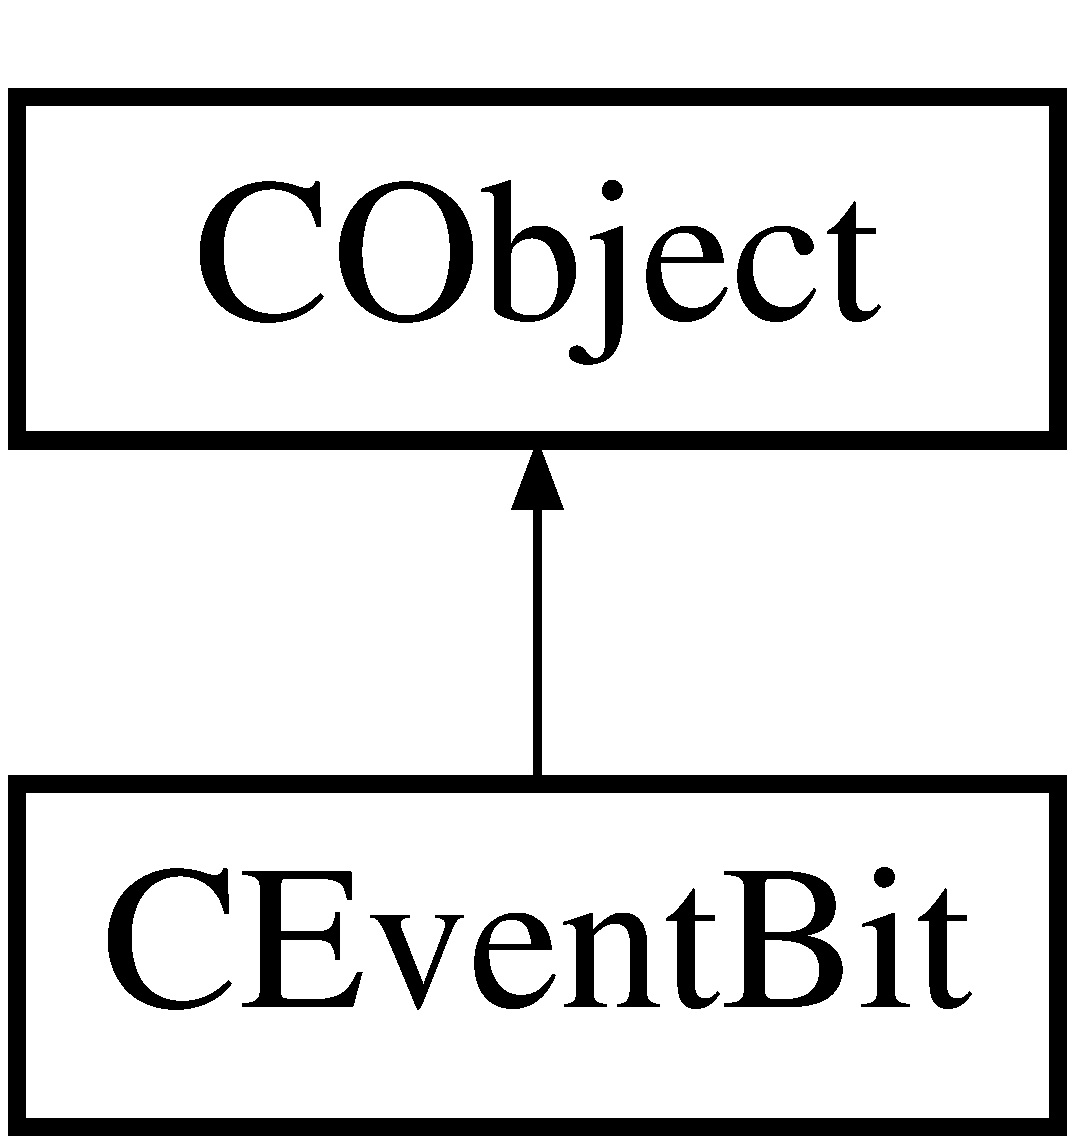
\includegraphics[height=2.000000cm]{class_c_event_bit}
\end{center}
\end{figure}
\subsection*{Public Member Functions}
\begin{DoxyCompactItemize}
\item 
\hypertarget{class_c_event_bit_a0b05da65aa8bb0b77dd75f0a84b8fbb0}{virtual uint32\-\_\-t {\bfseries set} (uint32\-\_\-t bits)}\label{class_c_event_bit_a0b05da65aa8bb0b77dd75f0a84b8fbb0}

\item 
\hypertarget{class_c_event_bit_ade8e4420bd49ab351417ca955bb293e3}{virtual uint32\-\_\-t {\bfseries clr} (uint32\-\_\-t bits)}\label{class_c_event_bit_ade8e4420bd49ab351417ca955bb293e3}

\item 
\hypertarget{class_c_event_bit_a52b137d375dbb670b2473222c8914081}{virtual uint32\-\_\-t {\bfseries get} ()}\label{class_c_event_bit_a52b137d375dbb670b2473222c8914081}

\item 
\hypertarget{class_c_event_bit_a4183fe9b9d9cc00cd0ae806c9aaba461}{virtual uint32\-\_\-t {\bfseries wait} (uint32\-\_\-t bits\-To\-Wait, bool clear\-On\-Exit=true, bool wait\-For\-All=true, uint32\-\_\-t timeout=M\-A\-X\-\_\-\-D\-E\-L\-A\-Y\-\_\-\-T\-I\-M\-E)}\label{class_c_event_bit_a4183fe9b9d9cc00cd0ae806c9aaba461}

\item 
\hypertarget{class_c_event_bit_a4a50fd1376946d508762fa00d01034ce}{virtual uint32\-\_\-t {\bfseries sync} (uint32\-\_\-t bits\-To\-Set, uint32\-\_\-t bits\-To\-Wait, uint32\-\_\-t timeout=M\-A\-X\-\_\-\-D\-E\-L\-A\-Y\-\_\-\-T\-I\-M\-E)}\label{class_c_event_bit_a4a50fd1376946d508762fa00d01034ce}

\end{DoxyCompactItemize}
\subsection*{Protected Attributes}
\begin{DoxyCompactItemize}
\item 
\hypertarget{class_c_event_bit_a99560a5eb8518d37c62dd30d3382c17e}{x\-Handle {\bfseries m\-\_\-event}}\label{class_c_event_bit_a99560a5eb8518d37c62dd30d3382c17e}

\end{DoxyCompactItemize}


The documentation for this class was generated from the following file\-:\begin{DoxyCompactItemize}
\item 
event.\-h\end{DoxyCompactItemize}

\hypertarget{class_c_i2_c}{\section{C\-I2\-C Class Reference}
\label{class_c_i2_c}\index{C\-I2\-C@{C\-I2\-C}}
}


{\ttfamily \#include $<$i2c.\-h$>$}

Inheritance diagram for C\-I2\-C\-:\begin{figure}[H]
\begin{center}
\leavevmode
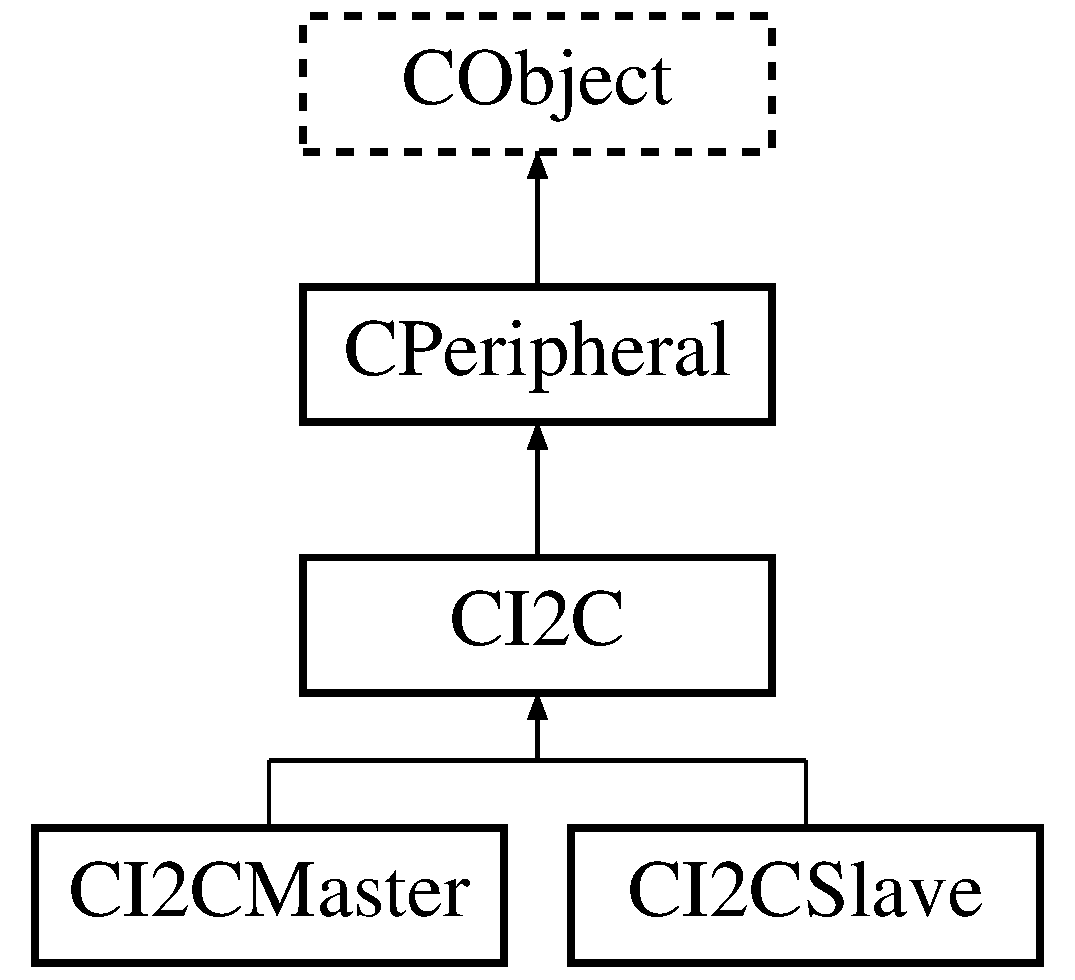
\includegraphics[height=4.000000cm]{d0/dce/class_c_i2_c}
\end{center}
\end{figure}
\subsection*{Public Member Functions}
\begin{DoxyCompactItemize}
\item 
\hyperlink{class_c_i2_c_a2df83a2627a8b8bf91460a68372c9ed5}{C\-I2\-C} ()
\item 
void \hyperlink{class_c_i2_c_aeff3f958457f68d453fe125b031c4539}{enable} ()
\item 
void \hyperlink{class_c_i2_c_a36a89b063ac68ff1710193258e76ea73}{disable} ()
\item 
virtual void \hyperlink{class_c_i2_c_ab5158b0fe99495c186200ac1d6ef4e52}{frequency} (uint32\-\_\-t hz)
\item 
virtual void \hyperlink{class_c_i2_c_a20801c3b9529bb0b3b29d51630a399de}{on\-State} (uint32\-\_\-t value)
\item 
virtual bool \hyperlink{class_c_i2_c_a1517b47af85f0129355d2242f124dfbc}{start} ()
\item 
virtual bool \hyperlink{class_c_i2_c_a68800b62b81e6fb291c24db5e0618e56}{stop} ()
\item 
virtual I2\-C\-\_\-\-E\-R\-R\-O\-R\-\_\-\-T \hyperlink{class_c_i2_c_ab0776700fc48c94f200774e832081c7f}{engine} (uint32\-\_\-t timeout=I2\-C\-\_\-\-T\-I\-M\-E\-O\-U\-T)
\item 
virtual void \hyperlink{class_c_i2_c_ac1730f4db280cd2c9b0d73a03317776e}{read} (uint8\-\_\-t $\ast$data, int length)
\item 
virtual void \hyperlink{class_c_i2_c_a379c419607c235a7d723ab4391c2ff2c}{write} (uint8\-\_\-t $\ast$data, int length)
\item 
virtual \hyperlink{class_c_i2_c_a1e66eebc5b74b3f79d44e506a6e72810}{$\sim$\-C\-I2\-C} ()
\end{DoxyCompactItemize}
\subsection*{Public Attributes}
\begin{DoxyCompactItemize}
\item 
\hyperlink{class_c_semaphore}{C\-Semaphore} \hyperlink{class_c_i2_c_afe268dd16ca42e8542c67a7f574df789}{m\-\_\-sem\-Irq}
\item 
\hyperlink{class_c_semaphore}{C\-Semaphore} \hyperlink{class_c_i2_c_aed6c05c74c281a6ae0dcc8e0203511b1}{m\-\_\-sem\-State}
\item 
uint32\-\_\-t \hyperlink{class_c_i2_c_aa2da331d3ad66d64a25d63405882be4c}{m\-\_\-state}
\item 
uint32\-\_\-t \hyperlink{class_c_i2_c_a4c29db1010457d99b12ac6097219bcc8}{m\-\_\-flag}
\item 
uint8\-\_\-t $\ast$ \hyperlink{class_c_i2_c_ae7fd0860329b89d55cfe5ca214b705e2}{m\-\_\-\-Master\-Buffer}
\item 
uint8\-\_\-t $\ast$ \hyperlink{class_c_i2_c_a4ef901e7efdef3f95faa2dd08d548aed}{m\-\_\-\-Slave\-Buffer}
\item 
int \hyperlink{class_c_i2_c_ad8b02ac3b8cfe93c0e123f7c4d79709b}{m\-\_\-rd\-Index}
\item 
int \hyperlink{class_c_i2_c_ad2e77f79779205f9c2ae13f7a4fc9168}{m\-\_\-wr\-Index}
\item 
int \hyperlink{class_c_i2_c_afc1ac8b1f15f1e74dd4a884fb9fe342a}{m\-\_\-wr\-Length}
\item 
int \hyperlink{class_c_i2_c_a517d08ec5c1a44662ab923bb74c6a25c}{m\-\_\-rd\-Length}
\end{DoxyCompactItemize}
\subsection*{Protected Attributes}
\begin{DoxyCompactItemize}
\item 
x\-Handle \hyperlink{class_c_i2_c_aef073fe282d448add47eb63b3f481205}{m\-\_\-handle}
\end{DoxyCompactItemize}


\subsection{Constructor \& Destructor Documentation}
\hypertarget{class_c_i2_c_a2df83a2627a8b8bf91460a68372c9ed5}{\index{C\-I2\-C@{C\-I2\-C}!C\-I2\-C@{C\-I2\-C}}
\index{C\-I2\-C@{C\-I2\-C}!CI2C@{C\-I2\-C}}
\subsubsection[{C\-I2\-C}]{\setlength{\rightskip}{0pt plus 5cm}C\-I2\-C\-::\-C\-I2\-C (
\begin{DoxyParamCaption}
{}
\end{DoxyParamCaption}
)}}\label{class_c_i2_c_a2df83a2627a8b8bf91460a68372c9ed5}
\hypertarget{class_c_i2_c_a1e66eebc5b74b3f79d44e506a6e72810}{\index{C\-I2\-C@{C\-I2\-C}!$\sim$\-C\-I2\-C@{$\sim$\-C\-I2\-C}}
\index{$\sim$\-C\-I2\-C@{$\sim$\-C\-I2\-C}!CI2C@{C\-I2\-C}}
\subsubsection[{$\sim$\-C\-I2\-C}]{\setlength{\rightskip}{0pt plus 5cm}virtual C\-I2\-C\-::$\sim$\-C\-I2\-C (
\begin{DoxyParamCaption}
{}
\end{DoxyParamCaption}
)\hspace{0.3cm}{\ttfamily [virtual]}}}\label{class_c_i2_c_a1e66eebc5b74b3f79d44e506a6e72810}


\subsection{Member Function Documentation}
\hypertarget{class_c_i2_c_aeff3f958457f68d453fe125b031c4539}{\index{C\-I2\-C@{C\-I2\-C}!enable@{enable}}
\index{enable@{enable}!CI2C@{C\-I2\-C}}
\subsubsection[{enable}]{\setlength{\rightskip}{0pt plus 5cm}void C\-I2\-C\-::enable (
\begin{DoxyParamCaption}
{}
\end{DoxyParamCaption}
)}}\label{class_c_i2_c_aeff3f958457f68d453fe125b031c4539}
\hypertarget{class_c_i2_c_a36a89b063ac68ff1710193258e76ea73}{\index{C\-I2\-C@{C\-I2\-C}!disable@{disable}}
\index{disable@{disable}!CI2C@{C\-I2\-C}}
\subsubsection[{disable}]{\setlength{\rightskip}{0pt plus 5cm}void C\-I2\-C\-::disable (
\begin{DoxyParamCaption}
{}
\end{DoxyParamCaption}
)}}\label{class_c_i2_c_a36a89b063ac68ff1710193258e76ea73}
\hypertarget{class_c_i2_c_ab5158b0fe99495c186200ac1d6ef4e52}{\index{C\-I2\-C@{C\-I2\-C}!frequency@{frequency}}
\index{frequency@{frequency}!CI2C@{C\-I2\-C}}
\subsubsection[{frequency}]{\setlength{\rightskip}{0pt plus 5cm}virtual void C\-I2\-C\-::frequency (
\begin{DoxyParamCaption}
\item[{uint32\-\_\-t}]{hz}
\end{DoxyParamCaption}
)\hspace{0.3cm}{\ttfamily [virtual]}}}\label{class_c_i2_c_ab5158b0fe99495c186200ac1d6ef4e52}
\hypertarget{class_c_i2_c_a20801c3b9529bb0b3b29d51630a399de}{\index{C\-I2\-C@{C\-I2\-C}!on\-State@{on\-State}}
\index{on\-State@{on\-State}!CI2C@{C\-I2\-C}}
\subsubsection[{on\-State}]{\setlength{\rightskip}{0pt plus 5cm}virtual void C\-I2\-C\-::on\-State (
\begin{DoxyParamCaption}
\item[{uint32\-\_\-t}]{value}
\end{DoxyParamCaption}
)\hspace{0.3cm}{\ttfamily [virtual]}}}\label{class_c_i2_c_a20801c3b9529bb0b3b29d51630a399de}
\hypertarget{class_c_i2_c_a1517b47af85f0129355d2242f124dfbc}{\index{C\-I2\-C@{C\-I2\-C}!start@{start}}
\index{start@{start}!CI2C@{C\-I2\-C}}
\subsubsection[{start}]{\setlength{\rightskip}{0pt plus 5cm}virtual bool C\-I2\-C\-::start (
\begin{DoxyParamCaption}
{}
\end{DoxyParamCaption}
)\hspace{0.3cm}{\ttfamily [virtual]}}}\label{class_c_i2_c_a1517b47af85f0129355d2242f124dfbc}
\hypertarget{class_c_i2_c_a68800b62b81e6fb291c24db5e0618e56}{\index{C\-I2\-C@{C\-I2\-C}!stop@{stop}}
\index{stop@{stop}!CI2C@{C\-I2\-C}}
\subsubsection[{stop}]{\setlength{\rightskip}{0pt plus 5cm}virtual bool C\-I2\-C\-::stop (
\begin{DoxyParamCaption}
{}
\end{DoxyParamCaption}
)\hspace{0.3cm}{\ttfamily [virtual]}}}\label{class_c_i2_c_a68800b62b81e6fb291c24db5e0618e56}
\hypertarget{class_c_i2_c_ab0776700fc48c94f200774e832081c7f}{\index{C\-I2\-C@{C\-I2\-C}!engine@{engine}}
\index{engine@{engine}!CI2C@{C\-I2\-C}}
\subsubsection[{engine}]{\setlength{\rightskip}{0pt plus 5cm}virtual I2\-C\-\_\-\-E\-R\-R\-O\-R\-\_\-\-T C\-I2\-C\-::engine (
\begin{DoxyParamCaption}
\item[{uint32\-\_\-t}]{timeout = {\ttfamily I2C\-\_\-TIMEOUT}}
\end{DoxyParamCaption}
)\hspace{0.3cm}{\ttfamily [virtual]}}}\label{class_c_i2_c_ab0776700fc48c94f200774e832081c7f}
\hypertarget{class_c_i2_c_ac1730f4db280cd2c9b0d73a03317776e}{\index{C\-I2\-C@{C\-I2\-C}!read@{read}}
\index{read@{read}!CI2C@{C\-I2\-C}}
\subsubsection[{read}]{\setlength{\rightskip}{0pt plus 5cm}virtual void C\-I2\-C\-::read (
\begin{DoxyParamCaption}
\item[{uint8\-\_\-t $\ast$}]{data, }
\item[{int}]{length}
\end{DoxyParamCaption}
)\hspace{0.3cm}{\ttfamily [virtual]}}}\label{class_c_i2_c_ac1730f4db280cd2c9b0d73a03317776e}
\hypertarget{class_c_i2_c_a379c419607c235a7d723ab4391c2ff2c}{\index{C\-I2\-C@{C\-I2\-C}!write@{write}}
\index{write@{write}!CI2C@{C\-I2\-C}}
\subsubsection[{write}]{\setlength{\rightskip}{0pt plus 5cm}virtual void C\-I2\-C\-::write (
\begin{DoxyParamCaption}
\item[{uint8\-\_\-t $\ast$}]{data, }
\item[{int}]{length}
\end{DoxyParamCaption}
)\hspace{0.3cm}{\ttfamily [virtual]}}}\label{class_c_i2_c_a379c419607c235a7d723ab4391c2ff2c}


\subsection{Member Data Documentation}
\hypertarget{class_c_i2_c_afe268dd16ca42e8542c67a7f574df789}{\index{C\-I2\-C@{C\-I2\-C}!m\-\_\-sem\-Irq@{m\-\_\-sem\-Irq}}
\index{m\-\_\-sem\-Irq@{m\-\_\-sem\-Irq}!CI2C@{C\-I2\-C}}
\subsubsection[{m\-\_\-sem\-Irq}]{\setlength{\rightskip}{0pt plus 5cm}{\bf C\-Semaphore} C\-I2\-C\-::m\-\_\-sem\-Irq}}\label{class_c_i2_c_afe268dd16ca42e8542c67a7f574df789}
\hypertarget{class_c_i2_c_aed6c05c74c281a6ae0dcc8e0203511b1}{\index{C\-I2\-C@{C\-I2\-C}!m\-\_\-sem\-State@{m\-\_\-sem\-State}}
\index{m\-\_\-sem\-State@{m\-\_\-sem\-State}!CI2C@{C\-I2\-C}}
\subsubsection[{m\-\_\-sem\-State}]{\setlength{\rightskip}{0pt plus 5cm}{\bf C\-Semaphore} C\-I2\-C\-::m\-\_\-sem\-State}}\label{class_c_i2_c_aed6c05c74c281a6ae0dcc8e0203511b1}
\hypertarget{class_c_i2_c_aa2da331d3ad66d64a25d63405882be4c}{\index{C\-I2\-C@{C\-I2\-C}!m\-\_\-state@{m\-\_\-state}}
\index{m\-\_\-state@{m\-\_\-state}!CI2C@{C\-I2\-C}}
\subsubsection[{m\-\_\-state}]{\setlength{\rightskip}{0pt plus 5cm}uint32\-\_\-t C\-I2\-C\-::m\-\_\-state}}\label{class_c_i2_c_aa2da331d3ad66d64a25d63405882be4c}
\hypertarget{class_c_i2_c_a4c29db1010457d99b12ac6097219bcc8}{\index{C\-I2\-C@{C\-I2\-C}!m\-\_\-flag@{m\-\_\-flag}}
\index{m\-\_\-flag@{m\-\_\-flag}!CI2C@{C\-I2\-C}}
\subsubsection[{m\-\_\-flag}]{\setlength{\rightskip}{0pt plus 5cm}uint32\-\_\-t C\-I2\-C\-::m\-\_\-flag}}\label{class_c_i2_c_a4c29db1010457d99b12ac6097219bcc8}
\hypertarget{class_c_i2_c_ae7fd0860329b89d55cfe5ca214b705e2}{\index{C\-I2\-C@{C\-I2\-C}!m\-\_\-\-Master\-Buffer@{m\-\_\-\-Master\-Buffer}}
\index{m\-\_\-\-Master\-Buffer@{m\-\_\-\-Master\-Buffer}!CI2C@{C\-I2\-C}}
\subsubsection[{m\-\_\-\-Master\-Buffer}]{\setlength{\rightskip}{0pt plus 5cm}uint8\-\_\-t$\ast$ C\-I2\-C\-::m\-\_\-\-Master\-Buffer}}\label{class_c_i2_c_ae7fd0860329b89d55cfe5ca214b705e2}
\hypertarget{class_c_i2_c_a4ef901e7efdef3f95faa2dd08d548aed}{\index{C\-I2\-C@{C\-I2\-C}!m\-\_\-\-Slave\-Buffer@{m\-\_\-\-Slave\-Buffer}}
\index{m\-\_\-\-Slave\-Buffer@{m\-\_\-\-Slave\-Buffer}!CI2C@{C\-I2\-C}}
\subsubsection[{m\-\_\-\-Slave\-Buffer}]{\setlength{\rightskip}{0pt plus 5cm}uint8\-\_\-t$\ast$ C\-I2\-C\-::m\-\_\-\-Slave\-Buffer}}\label{class_c_i2_c_a4ef901e7efdef3f95faa2dd08d548aed}
\hypertarget{class_c_i2_c_ad8b02ac3b8cfe93c0e123f7c4d79709b}{\index{C\-I2\-C@{C\-I2\-C}!m\-\_\-rd\-Index@{m\-\_\-rd\-Index}}
\index{m\-\_\-rd\-Index@{m\-\_\-rd\-Index}!CI2C@{C\-I2\-C}}
\subsubsection[{m\-\_\-rd\-Index}]{\setlength{\rightskip}{0pt plus 5cm}int C\-I2\-C\-::m\-\_\-rd\-Index}}\label{class_c_i2_c_ad8b02ac3b8cfe93c0e123f7c4d79709b}
\hypertarget{class_c_i2_c_ad2e77f79779205f9c2ae13f7a4fc9168}{\index{C\-I2\-C@{C\-I2\-C}!m\-\_\-wr\-Index@{m\-\_\-wr\-Index}}
\index{m\-\_\-wr\-Index@{m\-\_\-wr\-Index}!CI2C@{C\-I2\-C}}
\subsubsection[{m\-\_\-wr\-Index}]{\setlength{\rightskip}{0pt plus 5cm}int C\-I2\-C\-::m\-\_\-wr\-Index}}\label{class_c_i2_c_ad2e77f79779205f9c2ae13f7a4fc9168}
\hypertarget{class_c_i2_c_afc1ac8b1f15f1e74dd4a884fb9fe342a}{\index{C\-I2\-C@{C\-I2\-C}!m\-\_\-wr\-Length@{m\-\_\-wr\-Length}}
\index{m\-\_\-wr\-Length@{m\-\_\-wr\-Length}!CI2C@{C\-I2\-C}}
\subsubsection[{m\-\_\-wr\-Length}]{\setlength{\rightskip}{0pt plus 5cm}int C\-I2\-C\-::m\-\_\-wr\-Length}}\label{class_c_i2_c_afc1ac8b1f15f1e74dd4a884fb9fe342a}
\hypertarget{class_c_i2_c_a517d08ec5c1a44662ab923bb74c6a25c}{\index{C\-I2\-C@{C\-I2\-C}!m\-\_\-rd\-Length@{m\-\_\-rd\-Length}}
\index{m\-\_\-rd\-Length@{m\-\_\-rd\-Length}!CI2C@{C\-I2\-C}}
\subsubsection[{m\-\_\-rd\-Length}]{\setlength{\rightskip}{0pt plus 5cm}int C\-I2\-C\-::m\-\_\-rd\-Length}}\label{class_c_i2_c_a517d08ec5c1a44662ab923bb74c6a25c}
\hypertarget{class_c_i2_c_aef073fe282d448add47eb63b3f481205}{\index{C\-I2\-C@{C\-I2\-C}!m\-\_\-handle@{m\-\_\-handle}}
\index{m\-\_\-handle@{m\-\_\-handle}!CI2C@{C\-I2\-C}}
\subsubsection[{m\-\_\-handle}]{\setlength{\rightskip}{0pt plus 5cm}x\-Handle C\-I2\-C\-::m\-\_\-handle\hspace{0.3cm}{\ttfamily [protected]}}}\label{class_c_i2_c_aef073fe282d448add47eb63b3f481205}


The documentation for this class was generated from the following file\-:\begin{DoxyCompactItemize}
\item 
i2c.\-h\end{DoxyCompactItemize}

\hypertarget{class_c_i2_c_master}{\section{C\-I2\-C\-Master Class Reference}
\label{class_c_i2_c_master}\index{C\-I2\-C\-Master@{C\-I2\-C\-Master}}
}
Inheritance diagram for C\-I2\-C\-Master\-:\begin{figure}[H]
\begin{center}
\leavevmode
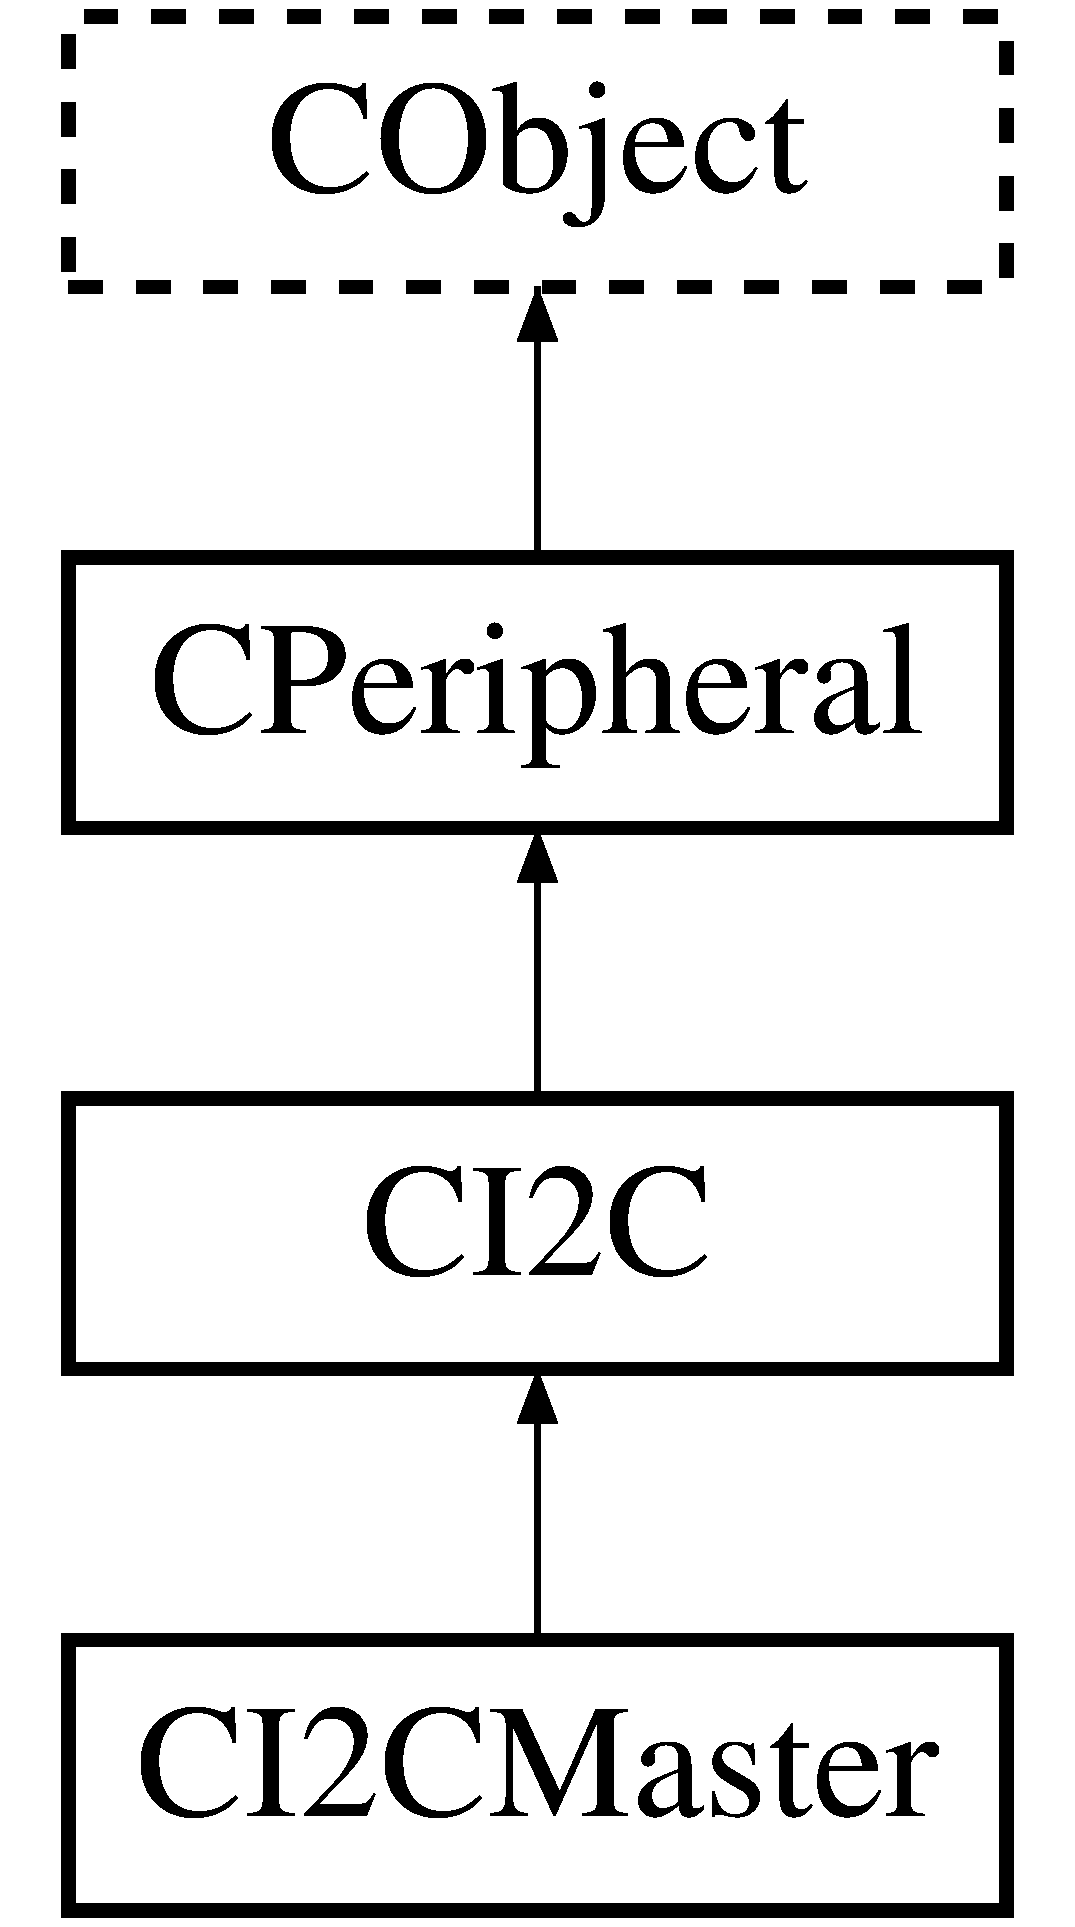
\includegraphics[height=4.000000cm]{class_c_i2_c_master}
\end{center}
\end{figure}
\subsection*{Public Member Functions}
\begin{DoxyCompactItemize}
\item 
\hypertarget{class_c_i2_c_master_aeea55afb38b9788048b5f7458616d208}{virtual I2\-C\-\_\-\-E\-R\-R\-O\-R\-\_\-\-T {\bfseries readwrite} (uint8\-\_\-t slave\-Addr, void $\ast$txbuf, int txsize, void $\ast$rxbuf, int rxsize)}\label{class_c_i2_c_master_aeea55afb38b9788048b5f7458616d208}

\end{DoxyCompactItemize}
\subsection*{Additional Inherited Members}


The documentation for this class was generated from the following file\-:\begin{DoxyCompactItemize}
\item 
i2c.\-h\end{DoxyCompactItemize}

\hypertarget{class_c_i2_c_slave}{\section{C\-I2\-C\-Slave Class Reference}
\label{class_c_i2_c_slave}\index{C\-I2\-C\-Slave@{C\-I2\-C\-Slave}}
}


{\ttfamily \#include $<$i2c.\-h$>$}

Inheritance diagram for C\-I2\-C\-Slave\-:\begin{figure}[H]
\begin{center}
\leavevmode
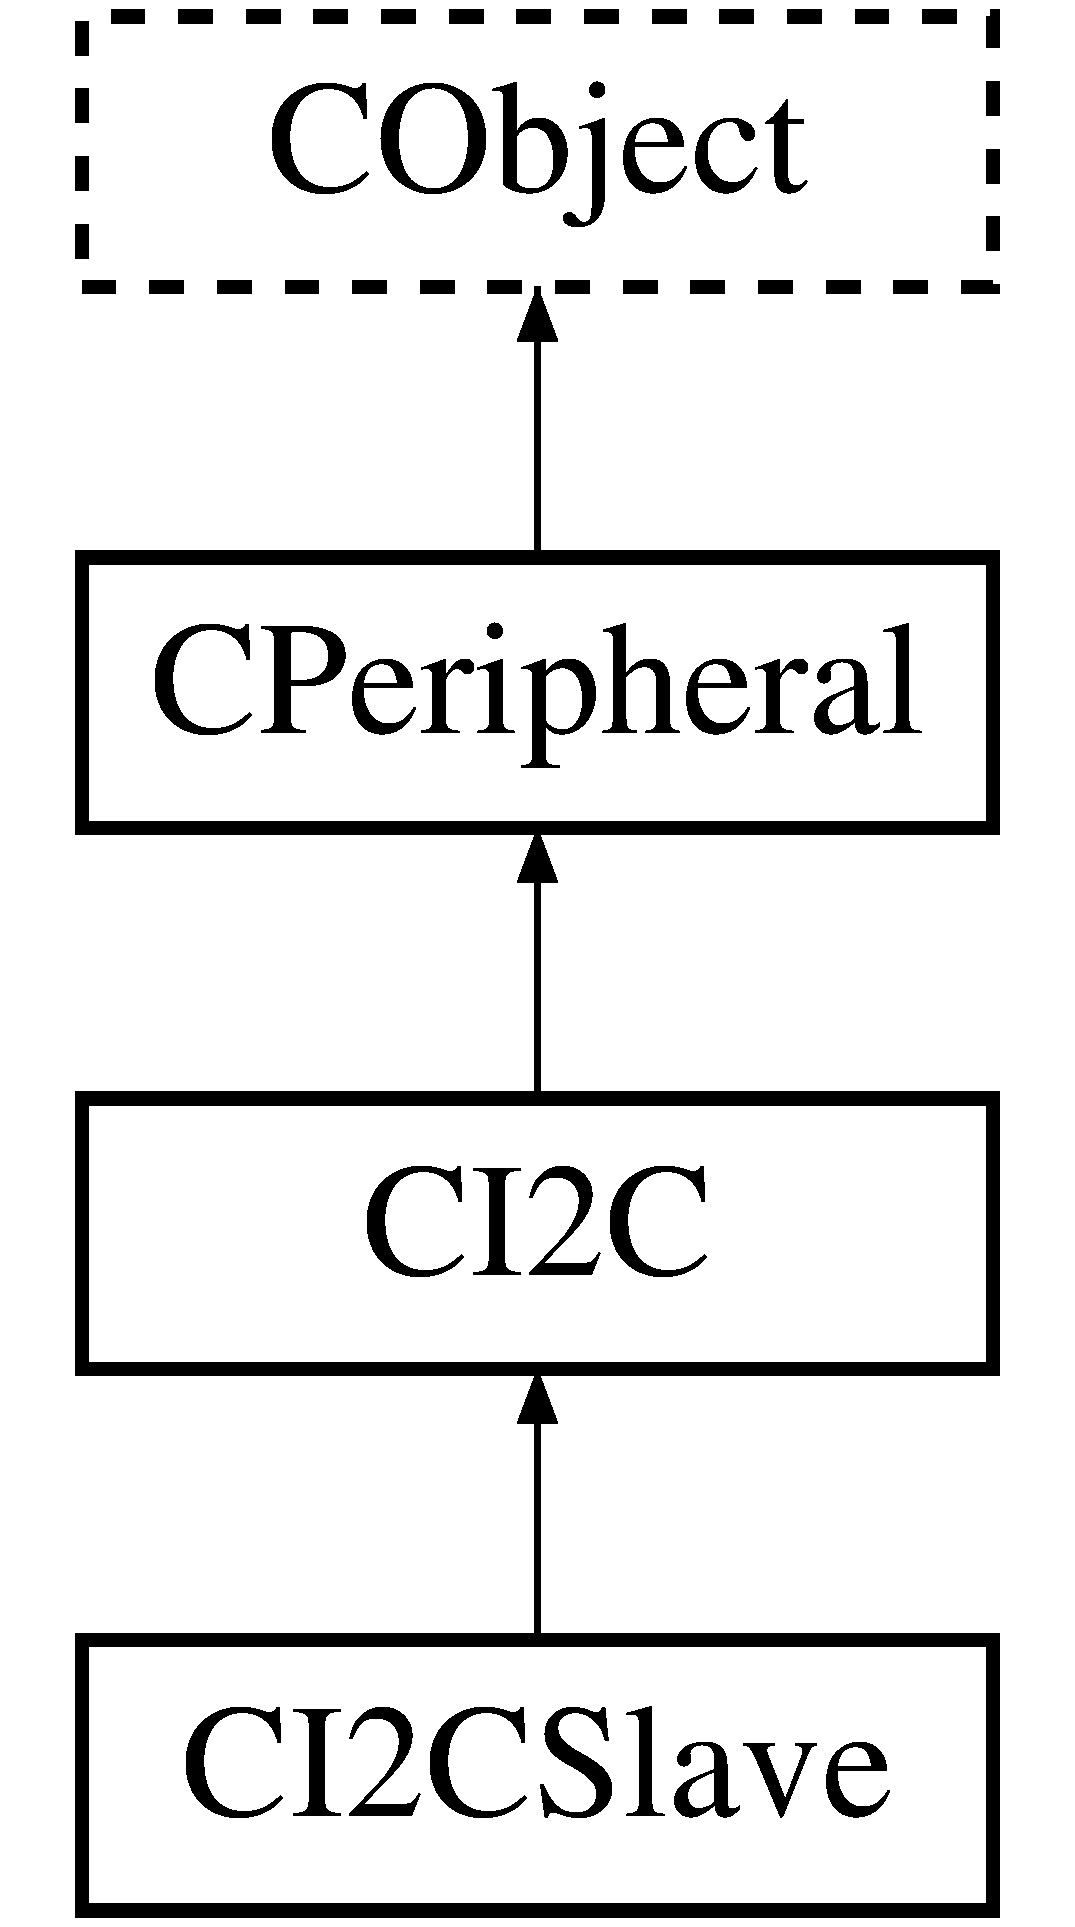
\includegraphics[height=4.000000cm]{d9/d52/class_c_i2_c_slave}
\end{center}
\end{figure}
\subsection*{Public Member Functions}
\begin{DoxyCompactItemize}
\item 
\hyperlink{class_c_i2_c_slave_adfd2a0e20a0560b382f423eb8a350aad}{C\-I2\-C\-Slave} (uint8\-\_\-t slave\-Addr)
\item 
virtual I2\-C\-\_\-\-E\-R\-R\-O\-R\-\_\-\-T \hyperlink{class_c_i2_c_slave_a1fe39972f6786151907517439c34acc3}{readwrite} (uint8\-\_\-t slave\-Addr, void $\ast$txbuf, int txsize, void $\ast$rxbuf, int rxsize)
\end{DoxyCompactItemize}
\subsection*{Additional Inherited Members}


\subsection{Constructor \& Destructor Documentation}
\hypertarget{class_c_i2_c_slave_adfd2a0e20a0560b382f423eb8a350aad}{\index{C\-I2\-C\-Slave@{C\-I2\-C\-Slave}!C\-I2\-C\-Slave@{C\-I2\-C\-Slave}}
\index{C\-I2\-C\-Slave@{C\-I2\-C\-Slave}!CI2CSlave@{C\-I2\-C\-Slave}}
\subsubsection[{C\-I2\-C\-Slave}]{\setlength{\rightskip}{0pt plus 5cm}C\-I2\-C\-Slave\-::\-C\-I2\-C\-Slave (
\begin{DoxyParamCaption}
\item[{uint8\-\_\-t}]{slave\-Addr}
\end{DoxyParamCaption}
)}}\label{class_c_i2_c_slave_adfd2a0e20a0560b382f423eb8a350aad}


\subsection{Member Function Documentation}
\hypertarget{class_c_i2_c_slave_a1fe39972f6786151907517439c34acc3}{\index{C\-I2\-C\-Slave@{C\-I2\-C\-Slave}!readwrite@{readwrite}}
\index{readwrite@{readwrite}!CI2CSlave@{C\-I2\-C\-Slave}}
\subsubsection[{readwrite}]{\setlength{\rightskip}{0pt plus 5cm}virtual I2\-C\-\_\-\-E\-R\-R\-O\-R\-\_\-\-T C\-I2\-C\-Slave\-::readwrite (
\begin{DoxyParamCaption}
\item[{uint8\-\_\-t}]{slave\-Addr, }
\item[{void $\ast$}]{txbuf, }
\item[{int}]{txsize, }
\item[{void $\ast$}]{rxbuf, }
\item[{int}]{rxsize}
\end{DoxyParamCaption}
)\hspace{0.3cm}{\ttfamily [virtual]}}}\label{class_c_i2_c_slave_a1fe39972f6786151907517439c34acc3}


The documentation for this class was generated from the following file\-:\begin{DoxyCompactItemize}
\item 
i2c.\-h\end{DoxyCompactItemize}

\hypertarget{class_c_list}{\section{C\-List Class Reference}
\label{class_c_list}\index{C\-List@{C\-List}}
}


{\ttfamily \#include $<$list.\-h$>$}

Inheritance diagram for C\-List\-:\begin{figure}[H]
\begin{center}
\leavevmode
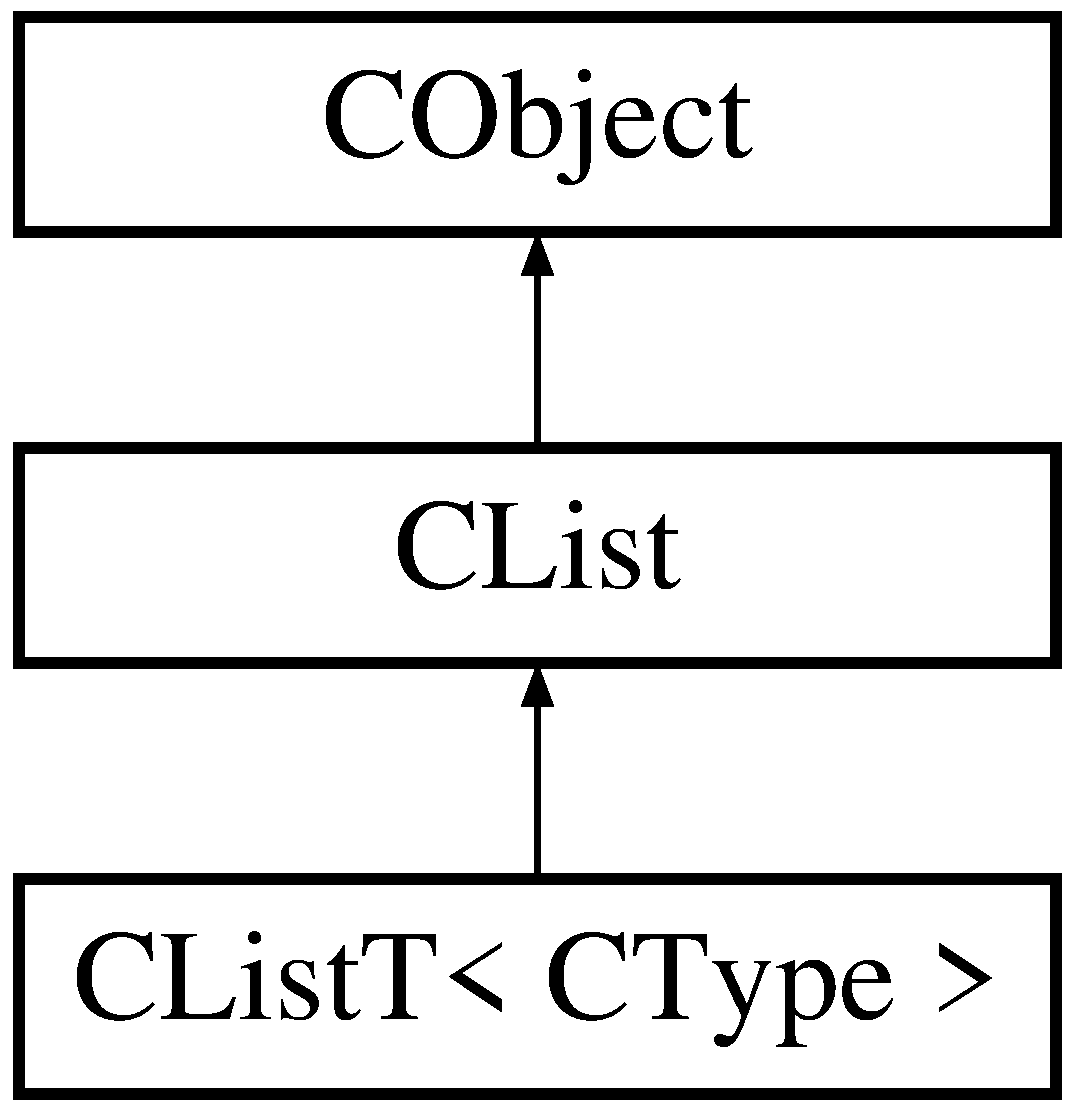
\includegraphics[height=3.000000cm]{df/db6/class_c_list}
\end{center}
\end{figure}
\subsection*{Public Member Functions}
\begin{DoxyCompactItemize}
\item 
\hyperlink{class_c_list_ae6434f79bc2d54fbd3617214a313af97}{C\-List} ()
\item 
virtual \hyperlink{class_c_list_aba485cb512089f00dcd7a08720d8e5de}{$\sim$\-C\-List} ()
\item 
virtual int \hyperlink{class_c_list_aba5942fb294f8f3381bef96ffc8f5054}{count} ()
\item 
virtual bool \hyperlink{class_c_list_ab4db98accd12debb4330ad97b8b1dc37}{is\-Empty} ()
\item 
virtual L\-I\-S\-T\-\_\-\-P\-O\-S \hyperlink{class_c_list_af77b9f95976788ad6b74e825fad12e94}{add\-Head} (E\-L\-E\-M\-\_\-\-P\-T\-R elem)
\item 
virtual L\-I\-S\-T\-\_\-\-P\-O\-S \hyperlink{class_c_list_a81c34b9127ccce385b6699b9eaa799d1}{add\-Tail} (E\-L\-E\-M\-\_\-\-P\-T\-R elem)
\item 
virtual E\-L\-E\-M\-\_\-\-P\-T\-R \hyperlink{class_c_list_acc4c74c1684f630c99988a477b0a3eb7}{get\-Head} ()
\item 
virtual E\-L\-E\-M\-\_\-\-P\-T\-R \hyperlink{class_c_list_a4bb6b07562fdd0cc376e7f300ed3b9c0}{get\-Tail} ()
\item 
virtual E\-L\-E\-M\-\_\-\-P\-T\-R \hyperlink{class_c_list_a54795f456c006f4ab3647d5abfaa806c}{get\-At} (L\-I\-S\-T\-\_\-\-P\-O\-S pos)
\item 
virtual E\-L\-E\-M\-\_\-\-P\-T\-R \hyperlink{class_c_list_abec03f2f356c1bcd44ff3ddfa3e1e65a}{get\-At} (int index)
\item 
virtual E\-L\-E\-M\-\_\-\-P\-T\-R \hyperlink{class_c_list_a0e0dfa3bc3d93b9708d4a454e91d0994}{remove\-Head} ()
\item 
virtual E\-L\-E\-M\-\_\-\-P\-T\-R \hyperlink{class_c_list_adc7cb308e77a9e0550eecce9333b071b}{remove\-Tail} ()
\item 
virtual E\-L\-E\-M\-\_\-\-P\-T\-R \hyperlink{class_c_list_a4baf624e719e27016de00005bbbc0f7b}{remove\-At} (L\-I\-S\-T\-\_\-\-P\-O\-S pos)
\item 
virtual void \hyperlink{class_c_list_a5ee3e7395c54395c7f603c08a1b9d5cf}{remove\-All} (bool free\-\_\-elem=false, bool is\-Obj=false)
\item 
virtual L\-I\-S\-T\-\_\-\-P\-O\-S \hyperlink{class_c_list_a9d1f8b32387ace522e2fa3a5bf68975a}{get\-Head\-Pos} ()
\item 
virtual L\-I\-S\-T\-\_\-\-P\-O\-S \hyperlink{class_c_list_a8cfadd6c7dd3dd6688e314b732e7b48f}{get\-Tail\-Pos} ()
\item 
virtual L\-I\-S\-T\-\_\-\-P\-O\-S \hyperlink{class_c_list_a30c0314e7dc83d1ba735f673b09e4deb}{get\-Next} (L\-I\-S\-T\-\_\-\-P\-O\-S pos)
\item 
virtual L\-I\-S\-T\-\_\-\-P\-O\-S \hyperlink{class_c_list_a4cf8035d25af022ba9c054c1b4f5b61c}{get\-Prev} (L\-I\-S\-T\-\_\-\-P\-O\-S pos)
\item 
virtual L\-I\-S\-T\-\_\-\-P\-O\-S \hyperlink{class_c_list_ac10ff6ad96cb1a7aebb866d2a1cf62bf}{find} (E\-L\-E\-M\-\_\-\-P\-T\-R elem)
\item 
virtual L\-I\-S\-T\-\_\-\-P\-O\-S \hyperlink{class_c_list_a02ae0a29f9466904e349a984d287a756}{insert\-Before} (L\-I\-S\-T\-\_\-\-P\-O\-S pos, E\-L\-E\-M\-\_\-\-P\-T\-R elem)
\item 
virtual L\-I\-S\-T\-\_\-\-P\-O\-S \hyperlink{class_c_list_ac30a5a1368438fbcf58b13bf4f2f44ad}{insert\-After} (L\-I\-S\-T\-\_\-\-P\-O\-S pos, E\-L\-E\-M\-\_\-\-P\-T\-R elem)
\item 
virtual E\-L\-E\-M\-\_\-\-P\-T\-R \hyperlink{class_c_list_aab328a02021b5988496f2dbb631bd71c}{operator\mbox{[}$\,$\mbox{]}} (int index)
\end{DoxyCompactItemize}
\subsection*{Protected Member Functions}
\begin{DoxyCompactItemize}
\item 
virtual L\-I\-S\-T\-\_\-\-P\-O\-S \hyperlink{class_c_list_acdb91815d21dabe0572e67da9bfd4c27}{alloc} ()
\item 
virtual void \hyperlink{class_c_list_aff212aceabad23dbb4370273ac91d814}{free} (L\-I\-S\-T\-\_\-\-P\-O\-S pos)
\end{DoxyCompactItemize}
\subsection*{Protected Attributes}
\begin{DoxyCompactItemize}
\item 
\hyperlink{class_c_mutex}{C\-Mutex} \hyperlink{class_c_list_a76347b2a51428a724cc7698074e08639}{m\-\_\-mutex}
\item 
L\-I\-S\-T\-\_\-\-P\-O\-S \hyperlink{class_c_list_a3ffa4c25b7b0604451366791aede5af7}{m\-\_\-nd\-Head}
\item 
L\-I\-S\-T\-\_\-\-P\-O\-S \hyperlink{class_c_list_aeeb0d3cb327800216a8f0fa112efa8d6}{m\-\_\-nd\-Tail}
\item 
int \hyperlink{class_c_list_adb228ed98190b1f57080840440f2eb2b}{length}
\end{DoxyCompactItemize}


\subsection{Constructor \& Destructor Documentation}
\hypertarget{class_c_list_ae6434f79bc2d54fbd3617214a313af97}{\index{C\-List@{C\-List}!C\-List@{C\-List}}
\index{C\-List@{C\-List}!CList@{C\-List}}
\subsubsection[{C\-List}]{\setlength{\rightskip}{0pt plus 5cm}C\-List\-::\-C\-List (
\begin{DoxyParamCaption}
{}
\end{DoxyParamCaption}
)}}\label{class_c_list_ae6434f79bc2d54fbd3617214a313af97}
\hypertarget{class_c_list_aba485cb512089f00dcd7a08720d8e5de}{\index{C\-List@{C\-List}!$\sim$\-C\-List@{$\sim$\-C\-List}}
\index{$\sim$\-C\-List@{$\sim$\-C\-List}!CList@{C\-List}}
\subsubsection[{$\sim$\-C\-List}]{\setlength{\rightskip}{0pt plus 5cm}virtual C\-List\-::$\sim$\-C\-List (
\begin{DoxyParamCaption}
{}
\end{DoxyParamCaption}
)\hspace{0.3cm}{\ttfamily [virtual]}}}\label{class_c_list_aba485cb512089f00dcd7a08720d8e5de}


\subsection{Member Function Documentation}
\hypertarget{class_c_list_acdb91815d21dabe0572e67da9bfd4c27}{\index{C\-List@{C\-List}!alloc@{alloc}}
\index{alloc@{alloc}!CList@{C\-List}}
\subsubsection[{alloc}]{\setlength{\rightskip}{0pt plus 5cm}virtual L\-I\-S\-T\-\_\-\-P\-O\-S C\-List\-::alloc (
\begin{DoxyParamCaption}
{}
\end{DoxyParamCaption}
)\hspace{0.3cm}{\ttfamily [protected]}, {\ttfamily [virtual]}}}\label{class_c_list_acdb91815d21dabe0572e67da9bfd4c27}
\hypertarget{class_c_list_aff212aceabad23dbb4370273ac91d814}{\index{C\-List@{C\-List}!free@{free}}
\index{free@{free}!CList@{C\-List}}
\subsubsection[{free}]{\setlength{\rightskip}{0pt plus 5cm}virtual void C\-List\-::free (
\begin{DoxyParamCaption}
\item[{L\-I\-S\-T\-\_\-\-P\-O\-S}]{pos}
\end{DoxyParamCaption}
)\hspace{0.3cm}{\ttfamily [protected]}, {\ttfamily [virtual]}}}\label{class_c_list_aff212aceabad23dbb4370273ac91d814}
\hypertarget{class_c_list_aba5942fb294f8f3381bef96ffc8f5054}{\index{C\-List@{C\-List}!count@{count}}
\index{count@{count}!CList@{C\-List}}
\subsubsection[{count}]{\setlength{\rightskip}{0pt plus 5cm}virtual int C\-List\-::count (
\begin{DoxyParamCaption}
{}
\end{DoxyParamCaption}
)\hspace{0.3cm}{\ttfamily [virtual]}}}\label{class_c_list_aba5942fb294f8f3381bef96ffc8f5054}
\hypertarget{class_c_list_ab4db98accd12debb4330ad97b8b1dc37}{\index{C\-List@{C\-List}!is\-Empty@{is\-Empty}}
\index{is\-Empty@{is\-Empty}!CList@{C\-List}}
\subsubsection[{is\-Empty}]{\setlength{\rightskip}{0pt plus 5cm}virtual bool C\-List\-::is\-Empty (
\begin{DoxyParamCaption}
{}
\end{DoxyParamCaption}
)\hspace{0.3cm}{\ttfamily [virtual]}}}\label{class_c_list_ab4db98accd12debb4330ad97b8b1dc37}
\hypertarget{class_c_list_af77b9f95976788ad6b74e825fad12e94}{\index{C\-List@{C\-List}!add\-Head@{add\-Head}}
\index{add\-Head@{add\-Head}!CList@{C\-List}}
\subsubsection[{add\-Head}]{\setlength{\rightskip}{0pt plus 5cm}virtual L\-I\-S\-T\-\_\-\-P\-O\-S C\-List\-::add\-Head (
\begin{DoxyParamCaption}
\item[{E\-L\-E\-M\-\_\-\-P\-T\-R}]{elem}
\end{DoxyParamCaption}
)\hspace{0.3cm}{\ttfamily [virtual]}}}\label{class_c_list_af77b9f95976788ad6b74e825fad12e94}
\hypertarget{class_c_list_a81c34b9127ccce385b6699b9eaa799d1}{\index{C\-List@{C\-List}!add\-Tail@{add\-Tail}}
\index{add\-Tail@{add\-Tail}!CList@{C\-List}}
\subsubsection[{add\-Tail}]{\setlength{\rightskip}{0pt plus 5cm}virtual L\-I\-S\-T\-\_\-\-P\-O\-S C\-List\-::add\-Tail (
\begin{DoxyParamCaption}
\item[{E\-L\-E\-M\-\_\-\-P\-T\-R}]{elem}
\end{DoxyParamCaption}
)\hspace{0.3cm}{\ttfamily [virtual]}}}\label{class_c_list_a81c34b9127ccce385b6699b9eaa799d1}
\hypertarget{class_c_list_acc4c74c1684f630c99988a477b0a3eb7}{\index{C\-List@{C\-List}!get\-Head@{get\-Head}}
\index{get\-Head@{get\-Head}!CList@{C\-List}}
\subsubsection[{get\-Head}]{\setlength{\rightskip}{0pt plus 5cm}virtual E\-L\-E\-M\-\_\-\-P\-T\-R C\-List\-::get\-Head (
\begin{DoxyParamCaption}
{}
\end{DoxyParamCaption}
)\hspace{0.3cm}{\ttfamily [virtual]}}}\label{class_c_list_acc4c74c1684f630c99988a477b0a3eb7}
\hypertarget{class_c_list_a4bb6b07562fdd0cc376e7f300ed3b9c0}{\index{C\-List@{C\-List}!get\-Tail@{get\-Tail}}
\index{get\-Tail@{get\-Tail}!CList@{C\-List}}
\subsubsection[{get\-Tail}]{\setlength{\rightskip}{0pt plus 5cm}virtual E\-L\-E\-M\-\_\-\-P\-T\-R C\-List\-::get\-Tail (
\begin{DoxyParamCaption}
{}
\end{DoxyParamCaption}
)\hspace{0.3cm}{\ttfamily [virtual]}}}\label{class_c_list_a4bb6b07562fdd0cc376e7f300ed3b9c0}
\hypertarget{class_c_list_a54795f456c006f4ab3647d5abfaa806c}{\index{C\-List@{C\-List}!get\-At@{get\-At}}
\index{get\-At@{get\-At}!CList@{C\-List}}
\subsubsection[{get\-At}]{\setlength{\rightskip}{0pt plus 5cm}virtual E\-L\-E\-M\-\_\-\-P\-T\-R C\-List\-::get\-At (
\begin{DoxyParamCaption}
\item[{L\-I\-S\-T\-\_\-\-P\-O\-S}]{pos}
\end{DoxyParamCaption}
)\hspace{0.3cm}{\ttfamily [virtual]}}}\label{class_c_list_a54795f456c006f4ab3647d5abfaa806c}
\hypertarget{class_c_list_abec03f2f356c1bcd44ff3ddfa3e1e65a}{\index{C\-List@{C\-List}!get\-At@{get\-At}}
\index{get\-At@{get\-At}!CList@{C\-List}}
\subsubsection[{get\-At}]{\setlength{\rightskip}{0pt plus 5cm}virtual E\-L\-E\-M\-\_\-\-P\-T\-R C\-List\-::get\-At (
\begin{DoxyParamCaption}
\item[{int}]{index}
\end{DoxyParamCaption}
)\hspace{0.3cm}{\ttfamily [virtual]}}}\label{class_c_list_abec03f2f356c1bcd44ff3ddfa3e1e65a}
\hypertarget{class_c_list_a0e0dfa3bc3d93b9708d4a454e91d0994}{\index{C\-List@{C\-List}!remove\-Head@{remove\-Head}}
\index{remove\-Head@{remove\-Head}!CList@{C\-List}}
\subsubsection[{remove\-Head}]{\setlength{\rightskip}{0pt plus 5cm}virtual E\-L\-E\-M\-\_\-\-P\-T\-R C\-List\-::remove\-Head (
\begin{DoxyParamCaption}
{}
\end{DoxyParamCaption}
)\hspace{0.3cm}{\ttfamily [virtual]}}}\label{class_c_list_a0e0dfa3bc3d93b9708d4a454e91d0994}
\hypertarget{class_c_list_adc7cb308e77a9e0550eecce9333b071b}{\index{C\-List@{C\-List}!remove\-Tail@{remove\-Tail}}
\index{remove\-Tail@{remove\-Tail}!CList@{C\-List}}
\subsubsection[{remove\-Tail}]{\setlength{\rightskip}{0pt plus 5cm}virtual E\-L\-E\-M\-\_\-\-P\-T\-R C\-List\-::remove\-Tail (
\begin{DoxyParamCaption}
{}
\end{DoxyParamCaption}
)\hspace{0.3cm}{\ttfamily [virtual]}}}\label{class_c_list_adc7cb308e77a9e0550eecce9333b071b}
\hypertarget{class_c_list_a4baf624e719e27016de00005bbbc0f7b}{\index{C\-List@{C\-List}!remove\-At@{remove\-At}}
\index{remove\-At@{remove\-At}!CList@{C\-List}}
\subsubsection[{remove\-At}]{\setlength{\rightskip}{0pt plus 5cm}virtual E\-L\-E\-M\-\_\-\-P\-T\-R C\-List\-::remove\-At (
\begin{DoxyParamCaption}
\item[{L\-I\-S\-T\-\_\-\-P\-O\-S}]{pos}
\end{DoxyParamCaption}
)\hspace{0.3cm}{\ttfamily [virtual]}}}\label{class_c_list_a4baf624e719e27016de00005bbbc0f7b}
\hypertarget{class_c_list_a5ee3e7395c54395c7f603c08a1b9d5cf}{\index{C\-List@{C\-List}!remove\-All@{remove\-All}}
\index{remove\-All@{remove\-All}!CList@{C\-List}}
\subsubsection[{remove\-All}]{\setlength{\rightskip}{0pt plus 5cm}virtual void C\-List\-::remove\-All (
\begin{DoxyParamCaption}
\item[{bool}]{free\-\_\-elem = {\ttfamily false}, }
\item[{bool}]{is\-Obj = {\ttfamily false}}
\end{DoxyParamCaption}
)\hspace{0.3cm}{\ttfamily [virtual]}}}\label{class_c_list_a5ee3e7395c54395c7f603c08a1b9d5cf}
\hypertarget{class_c_list_a9d1f8b32387ace522e2fa3a5bf68975a}{\index{C\-List@{C\-List}!get\-Head\-Pos@{get\-Head\-Pos}}
\index{get\-Head\-Pos@{get\-Head\-Pos}!CList@{C\-List}}
\subsubsection[{get\-Head\-Pos}]{\setlength{\rightskip}{0pt plus 5cm}virtual L\-I\-S\-T\-\_\-\-P\-O\-S C\-List\-::get\-Head\-Pos (
\begin{DoxyParamCaption}
{}
\end{DoxyParamCaption}
)\hspace{0.3cm}{\ttfamily [virtual]}}}\label{class_c_list_a9d1f8b32387ace522e2fa3a5bf68975a}
\hypertarget{class_c_list_a8cfadd6c7dd3dd6688e314b732e7b48f}{\index{C\-List@{C\-List}!get\-Tail\-Pos@{get\-Tail\-Pos}}
\index{get\-Tail\-Pos@{get\-Tail\-Pos}!CList@{C\-List}}
\subsubsection[{get\-Tail\-Pos}]{\setlength{\rightskip}{0pt plus 5cm}virtual L\-I\-S\-T\-\_\-\-P\-O\-S C\-List\-::get\-Tail\-Pos (
\begin{DoxyParamCaption}
{}
\end{DoxyParamCaption}
)\hspace{0.3cm}{\ttfamily [virtual]}}}\label{class_c_list_a8cfadd6c7dd3dd6688e314b732e7b48f}
\hypertarget{class_c_list_a30c0314e7dc83d1ba735f673b09e4deb}{\index{C\-List@{C\-List}!get\-Next@{get\-Next}}
\index{get\-Next@{get\-Next}!CList@{C\-List}}
\subsubsection[{get\-Next}]{\setlength{\rightskip}{0pt plus 5cm}virtual L\-I\-S\-T\-\_\-\-P\-O\-S C\-List\-::get\-Next (
\begin{DoxyParamCaption}
\item[{L\-I\-S\-T\-\_\-\-P\-O\-S}]{pos}
\end{DoxyParamCaption}
)\hspace{0.3cm}{\ttfamily [virtual]}}}\label{class_c_list_a30c0314e7dc83d1ba735f673b09e4deb}
\hypertarget{class_c_list_a4cf8035d25af022ba9c054c1b4f5b61c}{\index{C\-List@{C\-List}!get\-Prev@{get\-Prev}}
\index{get\-Prev@{get\-Prev}!CList@{C\-List}}
\subsubsection[{get\-Prev}]{\setlength{\rightskip}{0pt plus 5cm}virtual L\-I\-S\-T\-\_\-\-P\-O\-S C\-List\-::get\-Prev (
\begin{DoxyParamCaption}
\item[{L\-I\-S\-T\-\_\-\-P\-O\-S}]{pos}
\end{DoxyParamCaption}
)\hspace{0.3cm}{\ttfamily [virtual]}}}\label{class_c_list_a4cf8035d25af022ba9c054c1b4f5b61c}
\hypertarget{class_c_list_ac10ff6ad96cb1a7aebb866d2a1cf62bf}{\index{C\-List@{C\-List}!find@{find}}
\index{find@{find}!CList@{C\-List}}
\subsubsection[{find}]{\setlength{\rightskip}{0pt plus 5cm}virtual L\-I\-S\-T\-\_\-\-P\-O\-S C\-List\-::find (
\begin{DoxyParamCaption}
\item[{E\-L\-E\-M\-\_\-\-P\-T\-R}]{elem}
\end{DoxyParamCaption}
)\hspace{0.3cm}{\ttfamily [virtual]}}}\label{class_c_list_ac10ff6ad96cb1a7aebb866d2a1cf62bf}
\hypertarget{class_c_list_a02ae0a29f9466904e349a984d287a756}{\index{C\-List@{C\-List}!insert\-Before@{insert\-Before}}
\index{insert\-Before@{insert\-Before}!CList@{C\-List}}
\subsubsection[{insert\-Before}]{\setlength{\rightskip}{0pt plus 5cm}virtual L\-I\-S\-T\-\_\-\-P\-O\-S C\-List\-::insert\-Before (
\begin{DoxyParamCaption}
\item[{L\-I\-S\-T\-\_\-\-P\-O\-S}]{pos, }
\item[{E\-L\-E\-M\-\_\-\-P\-T\-R}]{elem}
\end{DoxyParamCaption}
)\hspace{0.3cm}{\ttfamily [virtual]}}}\label{class_c_list_a02ae0a29f9466904e349a984d287a756}
\hypertarget{class_c_list_ac30a5a1368438fbcf58b13bf4f2f44ad}{\index{C\-List@{C\-List}!insert\-After@{insert\-After}}
\index{insert\-After@{insert\-After}!CList@{C\-List}}
\subsubsection[{insert\-After}]{\setlength{\rightskip}{0pt plus 5cm}virtual L\-I\-S\-T\-\_\-\-P\-O\-S C\-List\-::insert\-After (
\begin{DoxyParamCaption}
\item[{L\-I\-S\-T\-\_\-\-P\-O\-S}]{pos, }
\item[{E\-L\-E\-M\-\_\-\-P\-T\-R}]{elem}
\end{DoxyParamCaption}
)\hspace{0.3cm}{\ttfamily [virtual]}}}\label{class_c_list_ac30a5a1368438fbcf58b13bf4f2f44ad}
\hypertarget{class_c_list_aab328a02021b5988496f2dbb631bd71c}{\index{C\-List@{C\-List}!operator\mbox{[}$\,$\mbox{]}@{operator[]}}
\index{operator\mbox{[}$\,$\mbox{]}@{operator[]}!CList@{C\-List}}
\subsubsection[{operator[]}]{\setlength{\rightskip}{0pt plus 5cm}virtual E\-L\-E\-M\-\_\-\-P\-T\-R C\-List\-::operator\mbox{[}$\,$\mbox{]} (
\begin{DoxyParamCaption}
\item[{int}]{index}
\end{DoxyParamCaption}
)\hspace{0.3cm}{\ttfamily [inline]}, {\ttfamily [virtual]}}}\label{class_c_list_aab328a02021b5988496f2dbb631bd71c}


\subsection{Member Data Documentation}
\hypertarget{class_c_list_a76347b2a51428a724cc7698074e08639}{\index{C\-List@{C\-List}!m\-\_\-mutex@{m\-\_\-mutex}}
\index{m\-\_\-mutex@{m\-\_\-mutex}!CList@{C\-List}}
\subsubsection[{m\-\_\-mutex}]{\setlength{\rightskip}{0pt plus 5cm}{\bf C\-Mutex} C\-List\-::m\-\_\-mutex\hspace{0.3cm}{\ttfamily [protected]}}}\label{class_c_list_a76347b2a51428a724cc7698074e08639}
\hypertarget{class_c_list_a3ffa4c25b7b0604451366791aede5af7}{\index{C\-List@{C\-List}!m\-\_\-nd\-Head@{m\-\_\-nd\-Head}}
\index{m\-\_\-nd\-Head@{m\-\_\-nd\-Head}!CList@{C\-List}}
\subsubsection[{m\-\_\-nd\-Head}]{\setlength{\rightskip}{0pt plus 5cm}L\-I\-S\-T\-\_\-\-P\-O\-S C\-List\-::m\-\_\-nd\-Head\hspace{0.3cm}{\ttfamily [protected]}}}\label{class_c_list_a3ffa4c25b7b0604451366791aede5af7}
\hypertarget{class_c_list_aeeb0d3cb327800216a8f0fa112efa8d6}{\index{C\-List@{C\-List}!m\-\_\-nd\-Tail@{m\-\_\-nd\-Tail}}
\index{m\-\_\-nd\-Tail@{m\-\_\-nd\-Tail}!CList@{C\-List}}
\subsubsection[{m\-\_\-nd\-Tail}]{\setlength{\rightskip}{0pt plus 5cm}L\-I\-S\-T\-\_\-\-P\-O\-S C\-List\-::m\-\_\-nd\-Tail\hspace{0.3cm}{\ttfamily [protected]}}}\label{class_c_list_aeeb0d3cb327800216a8f0fa112efa8d6}
\hypertarget{class_c_list_adb228ed98190b1f57080840440f2eb2b}{\index{C\-List@{C\-List}!length@{length}}
\index{length@{length}!CList@{C\-List}}
\subsubsection[{length}]{\setlength{\rightskip}{0pt plus 5cm}int C\-List\-::length\hspace{0.3cm}{\ttfamily [protected]}}}\label{class_c_list_adb228ed98190b1f57080840440f2eb2b}


The documentation for this class was generated from the following file\-:\begin{DoxyCompactItemize}
\item 
list.\-h\end{DoxyCompactItemize}

\hypertarget{class_c_list_t}{\section{C\-List\-T$<$ C\-Type $>$ Class Template Reference}
\label{class_c_list_t}\index{C\-List\-T$<$ C\-Type $>$@{C\-List\-T$<$ C\-Type $>$}}
}
Inheritance diagram for C\-List\-T$<$ C\-Type $>$\-:\begin{figure}[H]
\begin{center}
\leavevmode
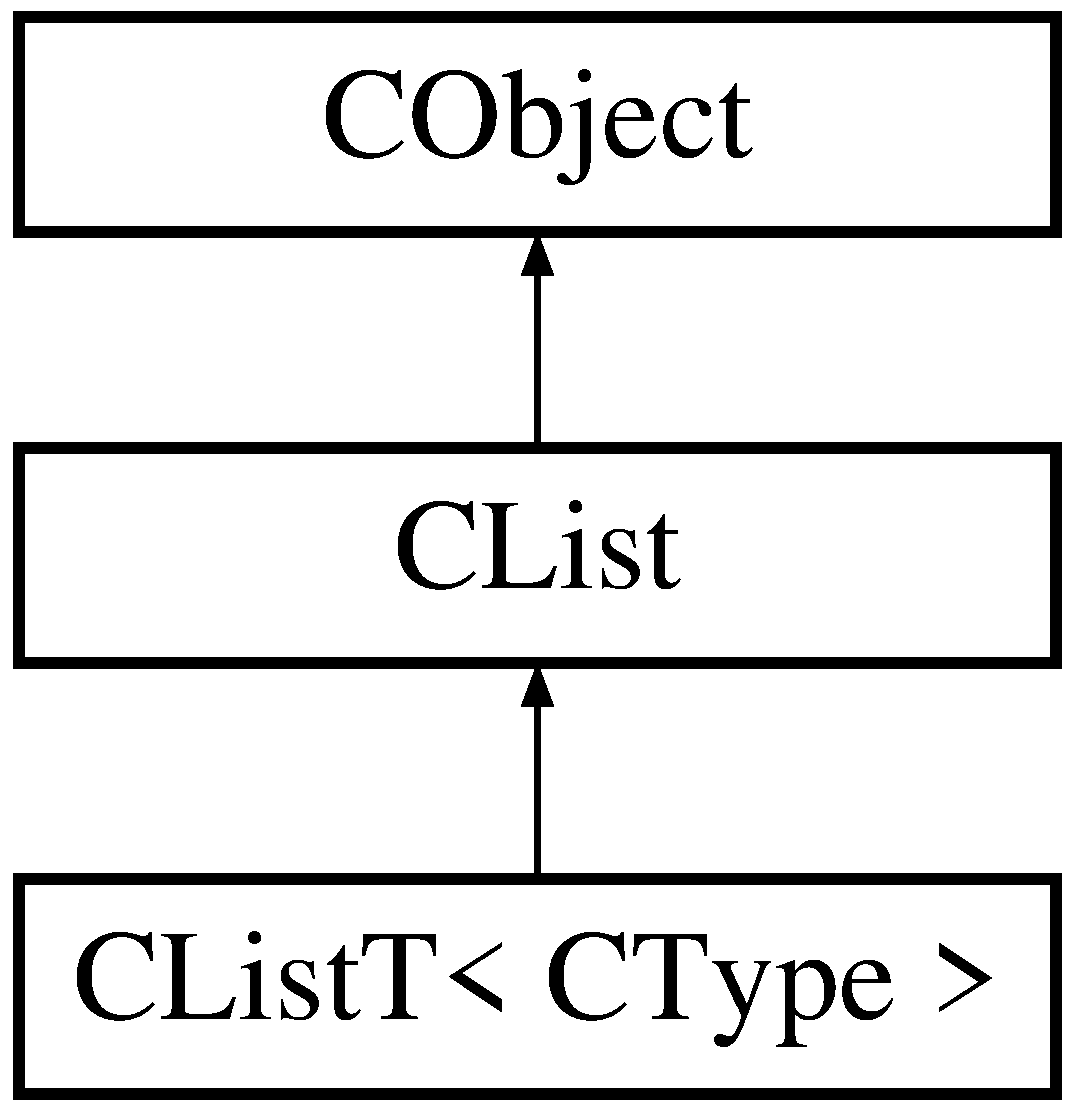
\includegraphics[height=3.000000cm]{class_c_list_t}
\end{center}
\end{figure}
\subsection*{Public Member Functions}
\begin{DoxyCompactItemize}
\item 
\hypertarget{class_c_list_t_a1135a93b349ac4ae024e45b8fbdc2842}{virtual L\-I\-S\-T\-\_\-\-P\-O\-S {\bfseries add\-Head\-T} (C\-Type $\ast$elem)}\label{class_c_list_t_a1135a93b349ac4ae024e45b8fbdc2842}

\item 
\hypertarget{class_c_list_t_a580d6fa5153806358134cda4fdd7810e}{virtual L\-I\-S\-T\-\_\-\-P\-O\-S {\bfseries add\-Tail\-T} (C\-Type $\ast$elem)}\label{class_c_list_t_a580d6fa5153806358134cda4fdd7810e}

\item 
\hypertarget{class_c_list_t_a4645ce0c83fb57db7b7c7b5baeff73ec}{virtual C\-Type $\ast$ {\bfseries get\-Head\-T} ()}\label{class_c_list_t_a4645ce0c83fb57db7b7c7b5baeff73ec}

\item 
\hypertarget{class_c_list_t_a3084c493b524681a3bc40be808bc5b93}{virtual C\-Type $\ast$ {\bfseries get\-Tail\-T} ()}\label{class_c_list_t_a3084c493b524681a3bc40be808bc5b93}

\item 
\hypertarget{class_c_list_t_a18acff60ba234e5f4e6728be0c66a171}{virtual C\-Type $\ast$ {\bfseries get\-At\-T} (L\-I\-S\-T\-\_\-\-P\-O\-S pos)}\label{class_c_list_t_a18acff60ba234e5f4e6728be0c66a171}

\item 
\hypertarget{class_c_list_t_a8d5f6f7d4251425a6583f4ffe6ccdd37}{virtual C\-Type $\ast$ {\bfseries remove\-Head\-T} ()}\label{class_c_list_t_a8d5f6f7d4251425a6583f4ffe6ccdd37}

\item 
\hypertarget{class_c_list_t_acb8c0cc7df7297b766065d3d89eba530}{virtual C\-Type $\ast$ {\bfseries remove\-Tail\-T} ()}\label{class_c_list_t_acb8c0cc7df7297b766065d3d89eba530}

\item 
\hypertarget{class_c_list_t_abf84e4b6b4cb035ea2a5c174acf8da45}{virtual void {\bfseries remove\-At\-T} (C\-Type $\ast$elem)}\label{class_c_list_t_abf84e4b6b4cb035ea2a5c174acf8da45}

\item 
\hypertarget{class_c_list_t_a33519401fb498e0b5f64e2da041726cc}{virtual void {\bfseries remove\-All\-T} (bool free\-\_\-elem=false)}\label{class_c_list_t_a33519401fb498e0b5f64e2da041726cc}

\item 
\hypertarget{class_c_list_t_affdeb2786698f49ea1dda928591cbc5e}{virtual L\-I\-S\-T\-\_\-\-P\-O\-S {\bfseries insert\-Before\-T} (L\-I\-S\-T\-\_\-\-P\-O\-S pos, C\-Type $\ast$elem)}\label{class_c_list_t_affdeb2786698f49ea1dda928591cbc5e}

\item 
\hypertarget{class_c_list_t_abcd6ee703a0256c5ecd6f04fd7c83e6b}{virtual L\-I\-S\-T\-\_\-\-P\-O\-S {\bfseries insert\-After\-T} (L\-I\-S\-T\-\_\-\-P\-O\-S pos, C\-Type $\ast$elem)}\label{class_c_list_t_abcd6ee703a0256c5ecd6f04fd7c83e6b}

\end{DoxyCompactItemize}
\subsection*{Additional Inherited Members}


The documentation for this class was generated from the following file\-:\begin{DoxyCompactItemize}
\item 
list.\-h\end{DoxyCompactItemize}

\hypertarget{class_c_mail_box}{\section{C\-Mail\-Box Class Reference}
\label{class_c_mail_box}\index{C\-Mail\-Box@{C\-Mail\-Box}}
}


{\ttfamily \#include \char`\"{}class/mailbox.\-h\char`\"{}}

Inheritance diagram for C\-Mail\-Box\-:\begin{figure}[H]
\begin{center}
\leavevmode
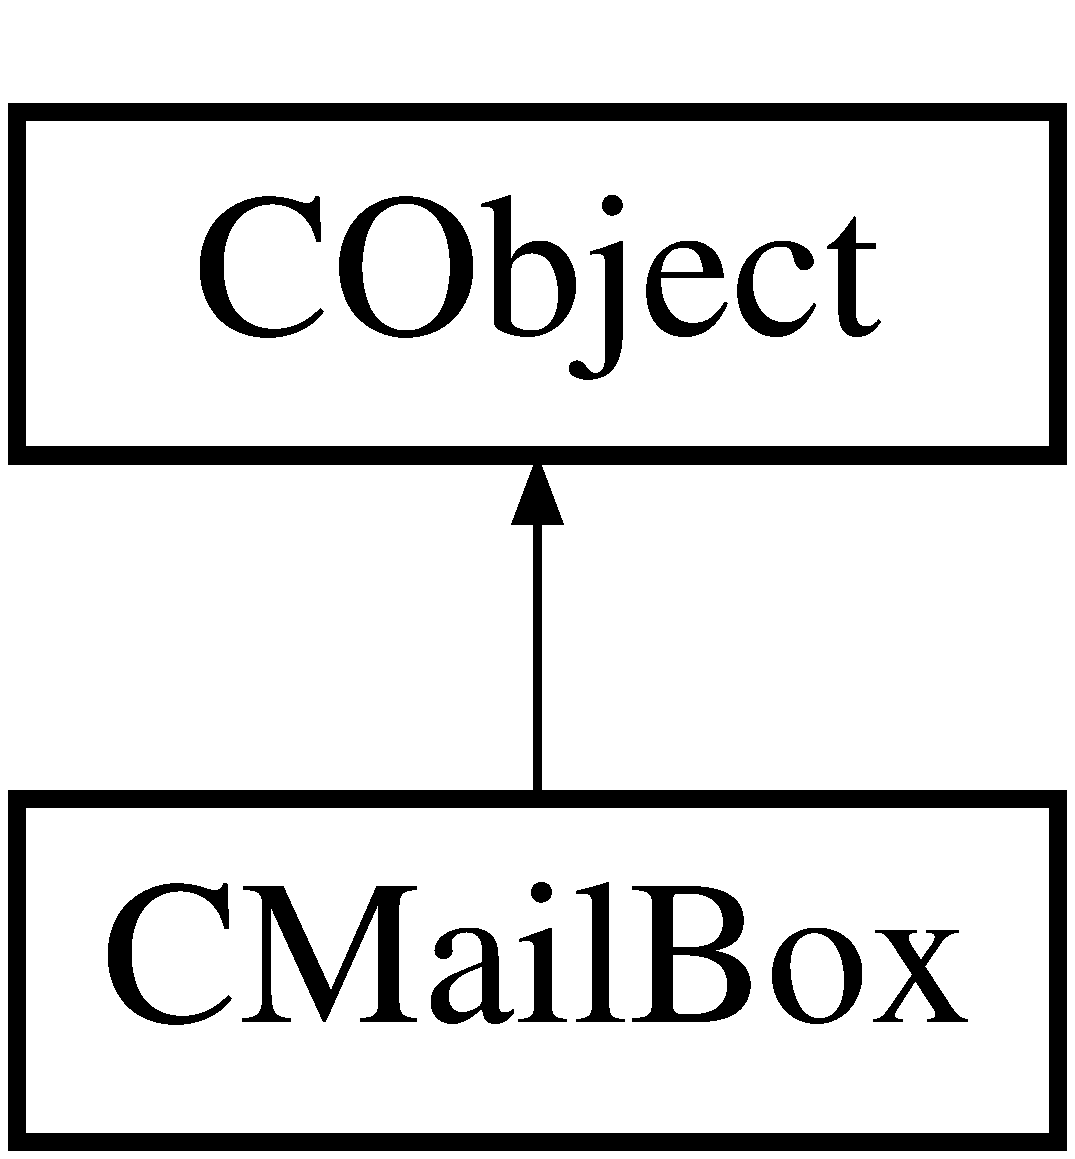
\includegraphics[height=2.000000cm]{d8/d26/class_c_mail_box}
\end{center}
\end{figure}
\subsection*{Public Member Functions}
\begin{DoxyCompactItemize}
\item 
\hyperlink{class_c_mail_box_a860c64ec622b6bb2641f8e69748ba9e6}{C\-Mail\-Box} (L\-P\-C\-T\-S\-T\-R name, int \hyperlink{class_c_mail_box_a11592da3e55cf9bedc8d2cf36d56e9bd}{count}=D\-E\-F\-\_\-\-M\-A\-I\-L\-\_\-\-C\-O\-U\-N\-T)
\item 
virtual M\-E\-S\-S\-A\-G\-E\-\_\-\-T \hyperlink{class_c_mail_box_ad03ed94ae07a9309d9f42695c9df7e94}{wait} (uint32\-\_\-t timeout=M\-A\-X\-\_\-\-D\-E\-L\-A\-Y\-\_\-\-T\-I\-M\-E)
\item 
virtual M\-E\-S\-S\-A\-G\-E\-\_\-\-T \hyperlink{class_c_mail_box_adc923a33209756bb2ed9e1838b12b68c}{peek} (uint32\-\_\-t timeout=M\-A\-X\-\_\-\-D\-E\-L\-A\-Y\-\_\-\-T\-I\-M\-E)
\item 
virtual int \hyperlink{class_c_mail_box_a11592da3e55cf9bedc8d2cf36d56e9bd}{count} ()
\item 
virtual bool \hyperlink{class_c_mail_box_a5ab581cd317944e824efbbc6f7f4d14d}{post} (M\-E\-S\-S\-A\-G\-E\-\_\-\-T msg, uint32\-\_\-t timeout=M\-A\-X\-\_\-\-D\-E\-L\-A\-Y\-\_\-\-T\-I\-M\-E)
\item 
void \hyperlink{class_c_mail_box_a73d5b694b1e7ce4e05c7ccc8f1dfd695}{reset} ()
\end{DoxyCompactItemize}
\subsection*{Static Public Member Functions}
\begin{DoxyCompactItemize}
\item 
static bool \hyperlink{class_c_mail_box_a96075bbd5308e6b1d0aaf5bd5fa2e645}{post} (L\-P\-C\-T\-S\-T\-R name, M\-E\-S\-S\-A\-G\-E\-\_\-\-T msg, uint32\-\_\-t timeout=0)
\end{DoxyCompactItemize}


\subsection{Detailed Description}
Use the C\-Mailbox to receive a message pointer from sender. 

\subsection{Constructor \& Destructor Documentation}
\hypertarget{class_c_mail_box_a860c64ec622b6bb2641f8e69748ba9e6}{\index{C\-Mail\-Box@{C\-Mail\-Box}!C\-Mail\-Box@{C\-Mail\-Box}}
\index{C\-Mail\-Box@{C\-Mail\-Box}!CMailBox@{C\-Mail\-Box}}
\subsubsection[{C\-Mail\-Box}]{\setlength{\rightskip}{0pt plus 5cm}C\-Mail\-Box\-::\-C\-Mail\-Box (
\begin{DoxyParamCaption}
\item[{L\-P\-C\-T\-S\-T\-R}]{name, }
\item[{int}]{count = {\ttfamily DEF\-\_\-MAIL\-\_\-COUNT}}
\end{DoxyParamCaption}
)}}\label{class_c_mail_box_a860c64ec622b6bb2641f8e69748ba9e6}
Constructs a \hyperlink{class_c_mail_box}{C\-Mail\-Box} object. 
\begin{DoxyParams}{Parameters}
{\em name} & is a string to point to describe the name of mailbox. \\
\hline
{\em count} & is a integer value to specified the maximum number of message can be contain.\\
\hline
\end{DoxyParams}

\begin{DoxyCode}
Example:
        \textcolor{keyword}{class }CLedTask: \textcolor{keyword}{public} \hyperlink{class_c_thread}{CThread} \{
        \textcolor{keyword}{protected}:
            \textcolor{keyword}{virtual} \textcolor{keywordtype}{void} run() \{
            \hyperlink{class_c_bus}{CBus} leds(LED2, LED3, LED4, END);
            \hyperlink{class_c_mail_box}{CMailBox} mail(\textcolor{stringliteral}{"LED"});
            \textcolor{keywordtype}{int} *i;
            \textcolor{keywordflow}{while}(1) \{
                i = (\textcolor{keywordtype}{int} *) mail.wait();
                \textcolor{keywordflow}{if} ( i ) \{
                    leds[*i] = !leds[*i];
                \}
            \}
            \}
    \};
\end{DoxyCode}
 

\subsection{Member Function Documentation}
\hypertarget{class_c_mail_box_ad03ed94ae07a9309d9f42695c9df7e94}{\index{C\-Mail\-Box@{C\-Mail\-Box}!wait@{wait}}
\index{wait@{wait}!CMailBox@{C\-Mail\-Box}}
\subsubsection[{wait}]{\setlength{\rightskip}{0pt plus 5cm}virtual M\-E\-S\-S\-A\-G\-E\-\_\-\-T C\-Mail\-Box\-::wait (
\begin{DoxyParamCaption}
\item[{uint32\-\_\-t}]{timeout = {\ttfamily MAX\-\_\-DELAY\-\_\-TIME}}
\end{DoxyParamCaption}
)\hspace{0.3cm}{\ttfamily [virtual]}}}\label{class_c_mail_box_ad03ed94ae07a9309d9f42695c9df7e94}
Call the member function to wait a message from sender. 
\begin{DoxyParams}{Parameters}
{\em timeout} & is an amount of time the task should block for a message to receive. \\
\hline
\end{DoxyParams}
\begin{DoxyReturn}{Returns}
M\-E\-S\-S\-A\-G\-E\-\_\-\-T 
\end{DoxyReturn}
\hypertarget{class_c_mail_box_adc923a33209756bb2ed9e1838b12b68c}{\index{C\-Mail\-Box@{C\-Mail\-Box}!peek@{peek}}
\index{peek@{peek}!CMailBox@{C\-Mail\-Box}}
\subsubsection[{peek}]{\setlength{\rightskip}{0pt plus 5cm}virtual M\-E\-S\-S\-A\-G\-E\-\_\-\-T C\-Mail\-Box\-::peek (
\begin{DoxyParamCaption}
\item[{uint32\-\_\-t}]{timeout = {\ttfamily MAX\-\_\-DELAY\-\_\-TIME}}
\end{DoxyParamCaption}
)\hspace{0.3cm}{\ttfamily [virtual]}}}\label{class_c_mail_box_adc923a33209756bb2ed9e1838b12b68c}
Receive a message from mail box without remove \hypertarget{class_c_mail_box_a11592da3e55cf9bedc8d2cf36d56e9bd}{\index{C\-Mail\-Box@{C\-Mail\-Box}!count@{count}}
\index{count@{count}!CMailBox@{C\-Mail\-Box}}
\subsubsection[{count}]{\setlength{\rightskip}{0pt plus 5cm}virtual int C\-Mail\-Box\-::count (
\begin{DoxyParamCaption}
{}
\end{DoxyParamCaption}
)\hspace{0.3cm}{\ttfamily [virtual]}}}\label{class_c_mail_box_a11592da3e55cf9bedc8d2cf36d56e9bd}
Call the member function to retrieve the number of message stored in the mailbox. \begin{DoxyReturn}{Returns}
number of message. 
\end{DoxyReturn}
\hypertarget{class_c_mail_box_a5ab581cd317944e824efbbc6f7f4d14d}{\index{C\-Mail\-Box@{C\-Mail\-Box}!post@{post}}
\index{post@{post}!CMailBox@{C\-Mail\-Box}}
\subsubsection[{post}]{\setlength{\rightskip}{0pt plus 5cm}virtual bool C\-Mail\-Box\-::post (
\begin{DoxyParamCaption}
\item[{M\-E\-S\-S\-A\-G\-E\-\_\-\-T}]{msg, }
\item[{uint32\-\_\-t}]{timeout = {\ttfamily MAX\-\_\-DELAY\-\_\-TIME}}
\end{DoxyParamCaption}
)\hspace{0.3cm}{\ttfamily [virtual]}}}\label{class_c_mail_box_a5ab581cd317944e824efbbc6f7f4d14d}
Call the member function to send a message to receiver \hypertarget{class_c_mail_box_a96075bbd5308e6b1d0aaf5bd5fa2e645}{\index{C\-Mail\-Box@{C\-Mail\-Box}!post@{post}}
\index{post@{post}!CMailBox@{C\-Mail\-Box}}
\subsubsection[{post}]{\setlength{\rightskip}{0pt plus 5cm}static bool C\-Mail\-Box\-::post (
\begin{DoxyParamCaption}
\item[{L\-P\-C\-T\-S\-T\-R}]{name, }
\item[{M\-E\-S\-S\-A\-G\-E\-\_\-\-T}]{msg, }
\item[{uint32\-\_\-t}]{timeout = {\ttfamily 0}}
\end{DoxyParamCaption}
)\hspace{0.3cm}{\ttfamily [static]}}}\label{class_c_mail_box_a96075bbd5308e6b1d0aaf5bd5fa2e645}
Call the member function to send a message to receiver which the same mailbox name. 
\begin{DoxyParams}{Parameters}
{\em name} & is a string to point to which the same name of mailbox to be received the message. \\
\hline
{\em msg} & is a pointer to the message (void$\ast$). \\
\hline
{\em timeout} & is a time to wait for post. (Default zero) \\
\hline
\end{DoxyParams}
\begin{DoxyReturn}{Returns}
true if post the message successful; otherwise, pose failed.
\end{DoxyReturn}

\begin{DoxyCode}
Example:
    \textcolor{keyword}{class }Task1: \textcolor{keyword}{public} \hyperlink{class_c_thread}{CThread} \{
    \textcolor{keyword}{protected}:
    \textcolor{keyword}{virtual} \textcolor{keywordtype}{void} run() \{
        \textcolor{keywordtype}{int} i=0;
        \textcolor{keywordflow}{while}(1) \{
            \hyperlink{class_c_mail_box_a5ab581cd317944e824efbbc6f7f4d14d}{CMailBox::post}(MAIL\_LED, &i);
            sleep(500);
        \}
    \}
 \};
\end{DoxyCode}
 \begin{DoxyRemark}{Remarks}
The \hyperlink{class_c_mail_box_a5ab581cd317944e824efbbc6f7f4d14d}{C\-Mail\-Box\-::post} is a static function. 
\end{DoxyRemark}
\hypertarget{class_c_mail_box_a73d5b694b1e7ce4e05c7ccc8f1dfd695}{\index{C\-Mail\-Box@{C\-Mail\-Box}!reset@{reset}}
\index{reset@{reset}!CMailBox@{C\-Mail\-Box}}
\subsubsection[{reset}]{\setlength{\rightskip}{0pt plus 5cm}void C\-Mail\-Box\-::reset (
\begin{DoxyParamCaption}
{}
\end{DoxyParamCaption}
)}}\label{class_c_mail_box_a73d5b694b1e7ce4e05c7ccc8f1dfd695}
Reset the mail box to original empty state. 

The documentation for this class was generated from the following file\-:\begin{DoxyCompactItemize}
\item 
mailbox.\-h\end{DoxyCompactItemize}

\hypertarget{class_c_mutex}{\section{C\-Mutex Class Reference}
\label{class_c_mutex}\index{C\-Mutex@{C\-Mutex}}
}


{\ttfamily \#include \char`\"{}class/mutex.\-h\char`\"{}}

Inheritance diagram for C\-Mutex\-:\begin{figure}[H]
\begin{center}
\leavevmode
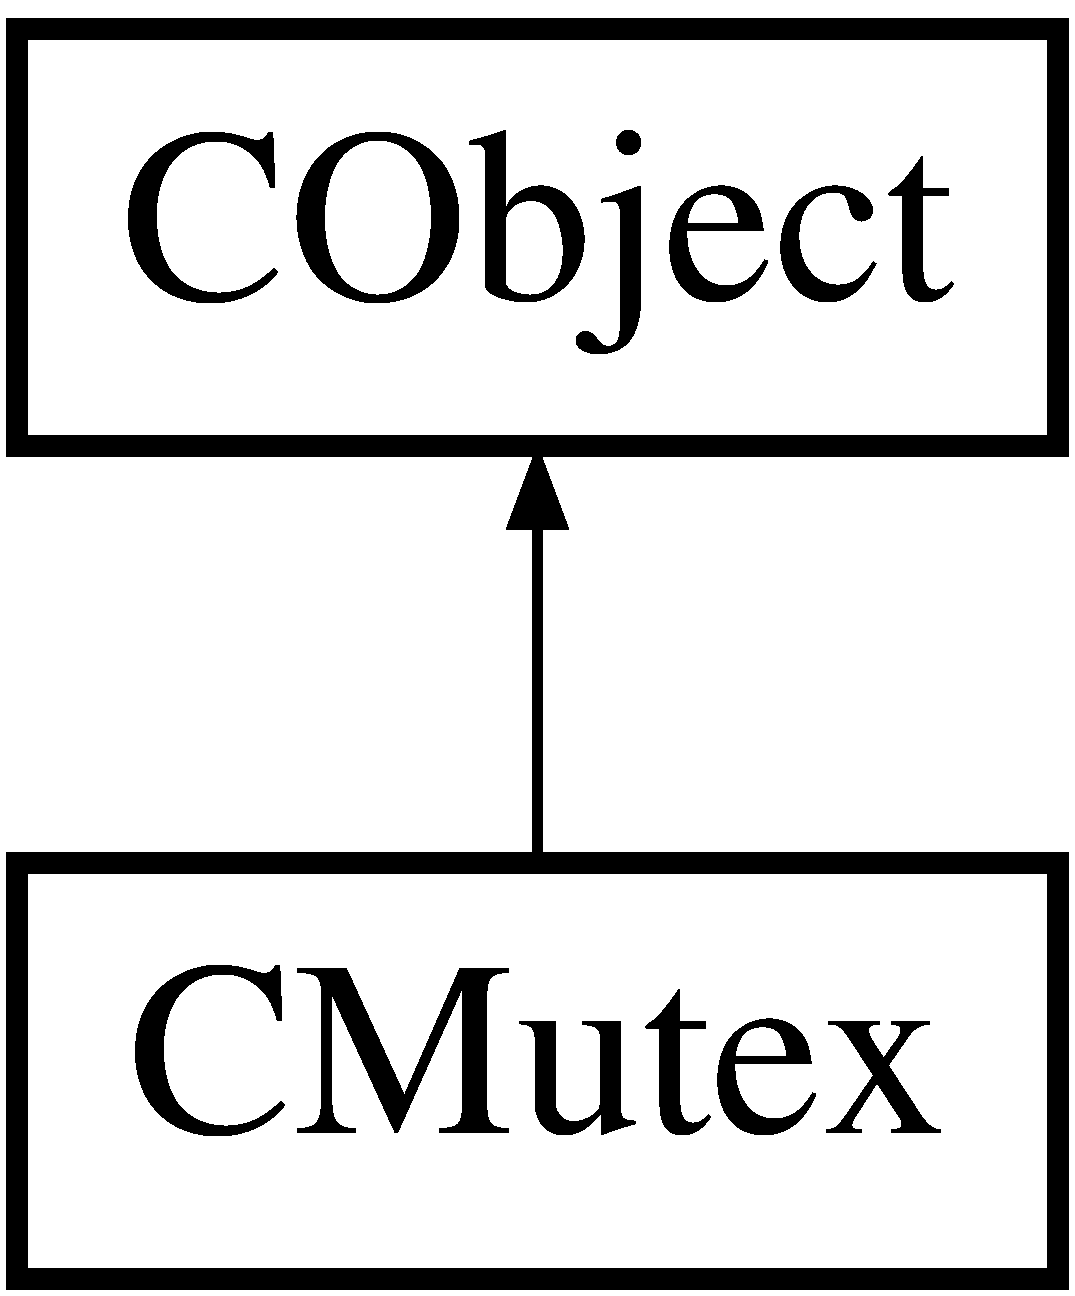
\includegraphics[height=2.000000cm]{d3/d0d/class_c_mutex}
\end{center}
\end{figure}
\subsection*{Public Member Functions}
\begin{DoxyCompactItemize}
\item 
virtual void \hyperlink{class_c_mutex_a820d77775dfd7d5dddfdac6bbf89b67a}{lock} ()
\item 
virtual bool \hyperlink{class_c_mutex_adb89cb4258a492458db9fb614c1681a9}{try\-Lock} (uint32\-\_\-t delay=0)
\item 
virtual void \hyperlink{class_c_mutex_aee0e6661ae4b790104a9a4205910d53d}{unlock} ()
\end{DoxyCompactItemize}


\subsection{Detailed Description}
Use the \hyperlink{class_c_mutex}{C\-Mutex} class to lock or unlock a resource. \begin{DoxyNote}{Note}
Mutexes and binary semaphores are very similar but have some subtle differences\-: Mutexes include a priority inheritance mechanism, binary semaphores do not. This makes binary semaphores the better choice for implementing synchronisation (between tasks or between tasks and an interrupt), and mutexes the better choice for implementing simple mutual exclusion. 
\end{DoxyNote}


\subsection{Member Function Documentation}
\hypertarget{class_c_mutex_a820d77775dfd7d5dddfdac6bbf89b67a}{\index{C\-Mutex@{C\-Mutex}!lock@{lock}}
\index{lock@{lock}!CMutex@{C\-Mutex}}
\subsubsection[{lock}]{\setlength{\rightskip}{0pt plus 5cm}virtual void C\-Mutex\-::lock (
\begin{DoxyParamCaption}
{}
\end{DoxyParamCaption}
)\hspace{0.3cm}{\ttfamily [virtual]}}}\label{class_c_mutex_a820d77775dfd7d5dddfdac6bbf89b67a}
Call the member function to lock (take semaphore) a resource with block when resource in used.


\begin{DoxyCode}
Example:
        \hyperlink{class_c_mutex}{CMutex} mutex;

        \hyperlink{class_c_serial}{CSerial} cdc(USB);
        \hyperlink{class_console}{Console} (cdc);

        \textcolor{keyword}{class }Task1: \textcolor{keyword}{public} \hyperlink{class_c_thread}{CThread} \{
        \textcolor{keyword}{protected}:
            \textcolor{keyword}{virtual} \textcolor{keywordtype}{void} run() \{
            \textcolor{keywordflow}{while}(1) \{
                \textcolor{keywordflow}{if} ( cdc.isConnected() ) \{
                    mutex.\hyperlink{class_c_mutex_a820d77775dfd7d5dddfdac6bbf89b67a}{lock}();
                    con << \textcolor{stringliteral}{"1111111111"} << endl;
                    mutex.\hyperlink{class_c_mutex_aee0e6661ae4b790104a9a4205910d53d}{unlock}();
                \}
            \}
            \}
        \};

        \textcolor{keyword}{class }Task2: \textcolor{keyword}{public} \hyperlink{class_c_thread}{CThread} \{
        \textcolor{keyword}{protected}:
            \textcolor{keyword}{virtual} \textcolor{keywordtype}{void} run() \{
            \textcolor{keywordflow}{while}(1) \{
                \textcolor{keywordflow}{if} ( cdc.isConnected() ) \{
                    mutex.\hyperlink{class_c_mutex_a820d77775dfd7d5dddfdac6bbf89b67a}{lock}();
                    con << \textcolor{stringliteral}{"2222222222"} << endl;
                    mutex.\hyperlink{class_c_mutex_aee0e6661ae4b790104a9a4205910d53d}{unlock}();
                \}
            \}
            \}
        \};
\end{DoxyCode}
 \hypertarget{class_c_mutex_adb89cb4258a492458db9fb614c1681a9}{\index{C\-Mutex@{C\-Mutex}!try\-Lock@{try\-Lock}}
\index{try\-Lock@{try\-Lock}!CMutex@{C\-Mutex}}
\subsubsection[{try\-Lock}]{\setlength{\rightskip}{0pt plus 5cm}virtual bool C\-Mutex\-::try\-Lock (
\begin{DoxyParamCaption}
\item[{uint32\-\_\-t}]{delay = {\ttfamily 0}}
\end{DoxyParamCaption}
)\hspace{0.3cm}{\ttfamily [virtual]}}}\label{class_c_mutex_adb89cb4258a492458db9fb614c1681a9}
Call the member function to lock (take) a resource without block when resource in used. \begin{DoxyReturn}{Returns}
true if lock successful; otherwise, failed. 
\end{DoxyReturn}
\hypertarget{class_c_mutex_aee0e6661ae4b790104a9a4205910d53d}{\index{C\-Mutex@{C\-Mutex}!unlock@{unlock}}
\index{unlock@{unlock}!CMutex@{C\-Mutex}}
\subsubsection[{unlock}]{\setlength{\rightskip}{0pt plus 5cm}virtual void C\-Mutex\-::unlock (
\begin{DoxyParamCaption}
{}
\end{DoxyParamCaption}
)\hspace{0.3cm}{\ttfamily [virtual]}}}\label{class_c_mutex_aee0e6661ae4b790104a9a4205910d53d}
Call the member function to unlock (release) a resource.


\begin{DoxyCode}
Example:
        \hyperlink{class_c_mutex}{CMutex} mutex;

        \hyperlink{class_c_serial}{CSerial} cdc(USB);
        \hyperlink{class_console}{Console} (cdc);

        \textcolor{keyword}{class }Task1: \textcolor{keyword}{public} \hyperlink{class_c_thread}{CThread} \{
        \textcolor{keyword}{protected}:
            \textcolor{keyword}{virtual} \textcolor{keywordtype}{void} run() \{
            \textcolor{keywordflow}{while}(1) \{
                \textcolor{keywordflow}{if} ( cdc.isConnected() ) \{
                    mutex.\hyperlink{class_c_mutex_a820d77775dfd7d5dddfdac6bbf89b67a}{lock}();
                    con << \textcolor{stringliteral}{"1111111111"} << endl;
                    mutex.\hyperlink{class_c_mutex_aee0e6661ae4b790104a9a4205910d53d}{unlock}();
                \}
            \}
            \}
        \};

        \textcolor{keyword}{class }Task2: \textcolor{keyword}{public} \hyperlink{class_c_thread}{CThread} \{
        \textcolor{keyword}{protected}:
            \textcolor{keyword}{virtual} \textcolor{keywordtype}{void} run() \{
            \textcolor{keywordflow}{while}(1) \{
                \textcolor{keywordflow}{if} ( cdc.isConnected() ) \{
                    mutex.\hyperlink{class_c_mutex_a820d77775dfd7d5dddfdac6bbf89b67a}{lock}();
                    con << \textcolor{stringliteral}{"2222222222"} << endl;
                    mutex.\hyperlink{class_c_mutex_aee0e6661ae4b790104a9a4205910d53d}{unlock}();
                \}
            \}
            \}
        \};
\end{DoxyCode}
 

The documentation for this class was generated from the following file\-:\begin{DoxyCompactItemize}
\item 
mutex.\-h\end{DoxyCompactItemize}

\hypertarget{class_c_object}{\section{C\-Object Class Reference}
\label{class_c_object}\index{C\-Object@{C\-Object}}
}
Inheritance diagram for C\-Object\-:\begin{figure}[H]
\begin{center}
\leavevmode
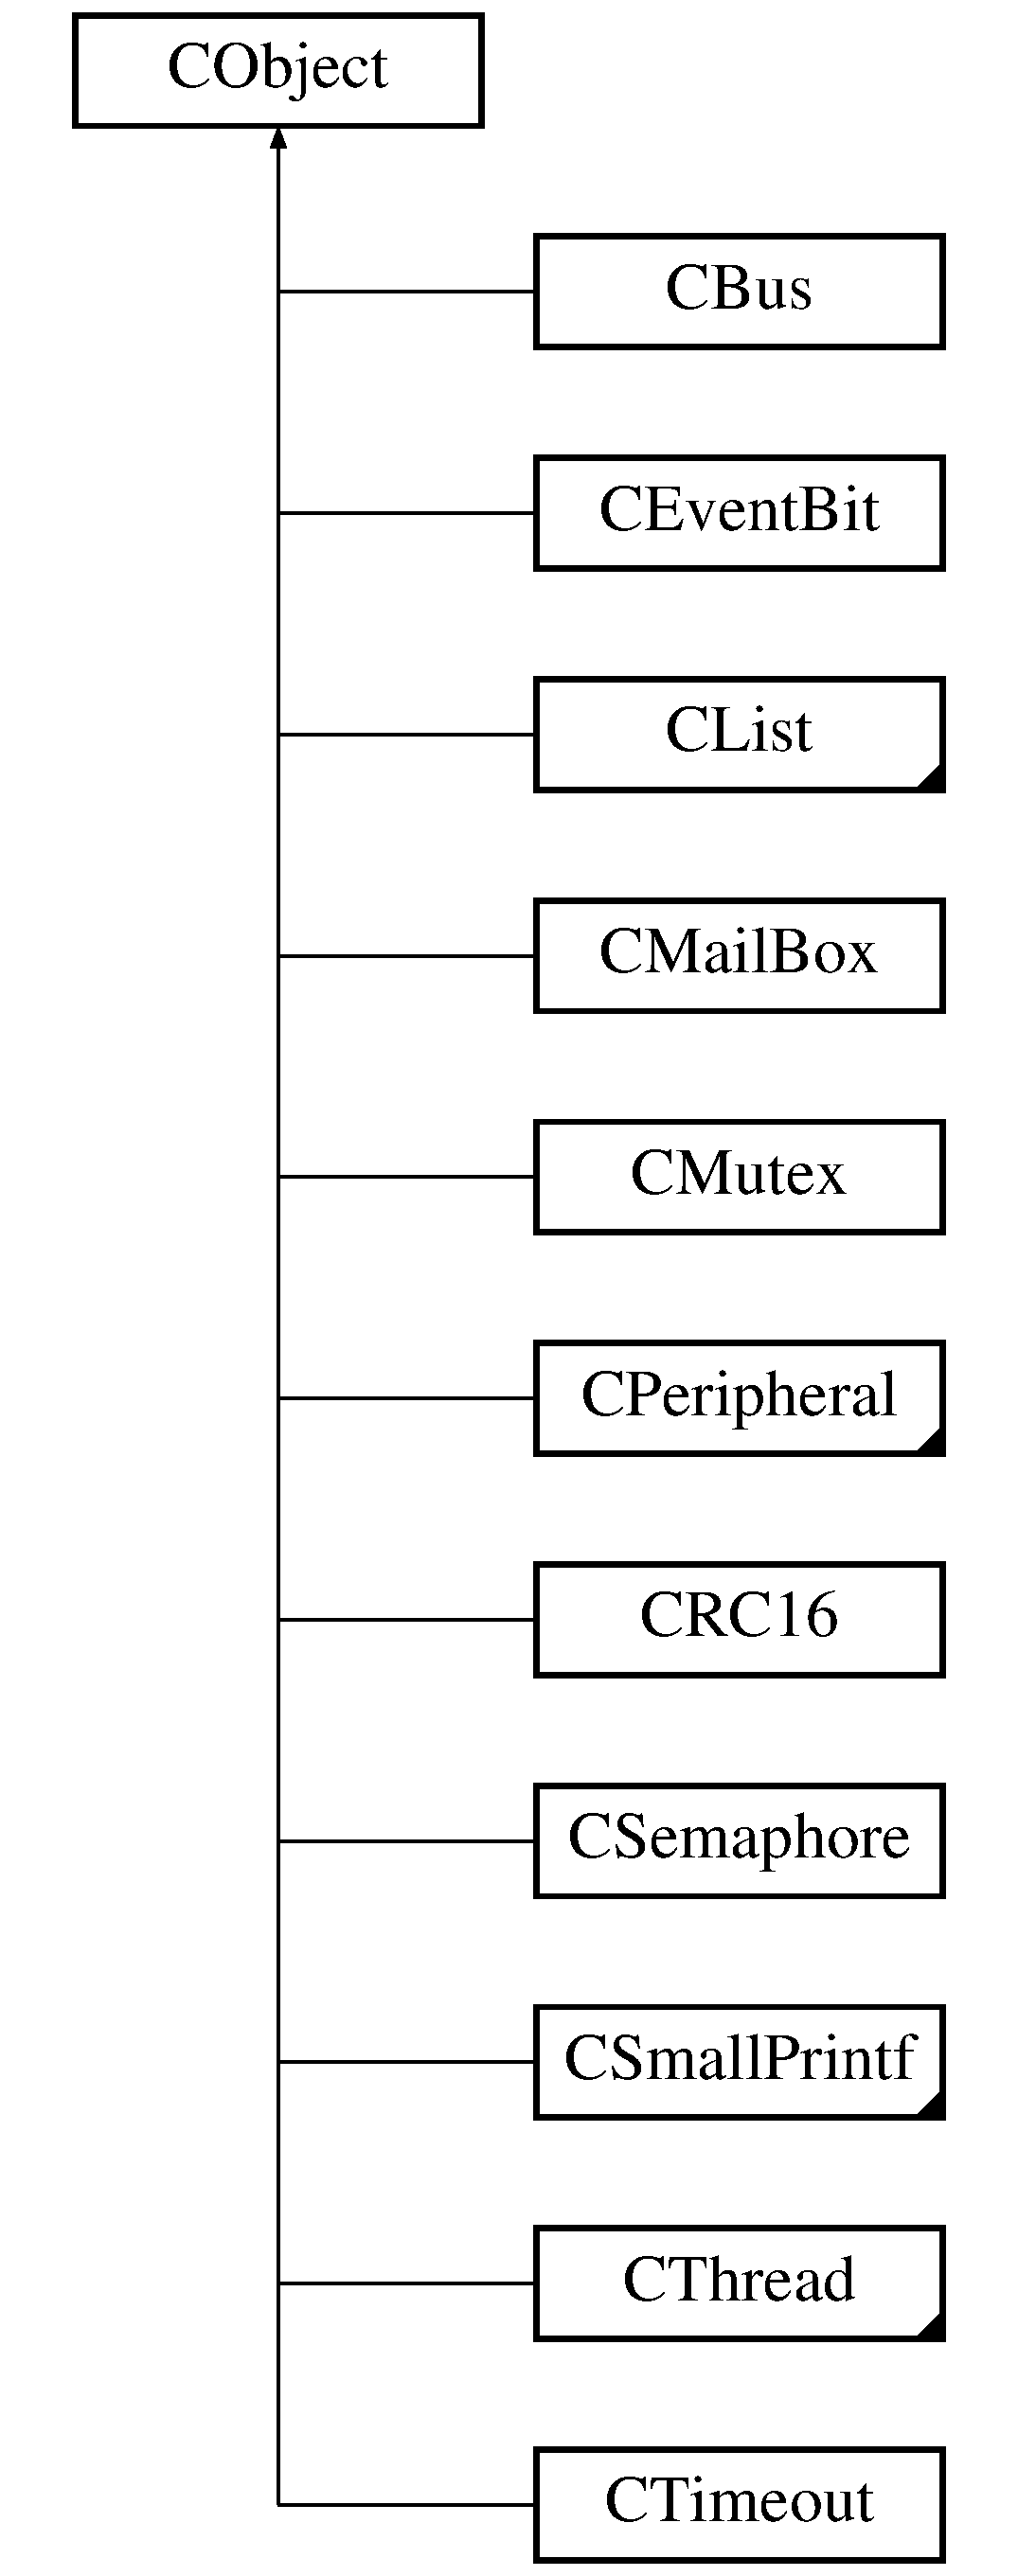
\includegraphics[height=12.000000cm]{class_c_object}
\end{center}
\end{figure}
\subsection*{Public Member Functions}
\begin{DoxyCompactItemize}
\item 
\hypertarget{class_c_object_a26a76c241a4d62d2efdac57d2cfe4c0f}{virtual bool {\bfseries is\-Thread} ()}\label{class_c_object_a26a76c241a4d62d2efdac57d2cfe4c0f}

\end{DoxyCompactItemize}


The documentation for this class was generated from the following file\-:\begin{DoxyCompactItemize}
\item 
object.\-h\end{DoxyCompactItemize}

\hypertarget{class_console}{\section{Console Class Reference}
\label{class_console}\index{Console@{Console}}
}


The \hyperlink{class_console}{Console} class provides a lightweight input/output stream to console.  




{\ttfamily \#include \char`\"{}class/console.\-h\char`\"{}}

Inheritance diagram for Console\-:\begin{figure}[H]
\begin{center}
\leavevmode
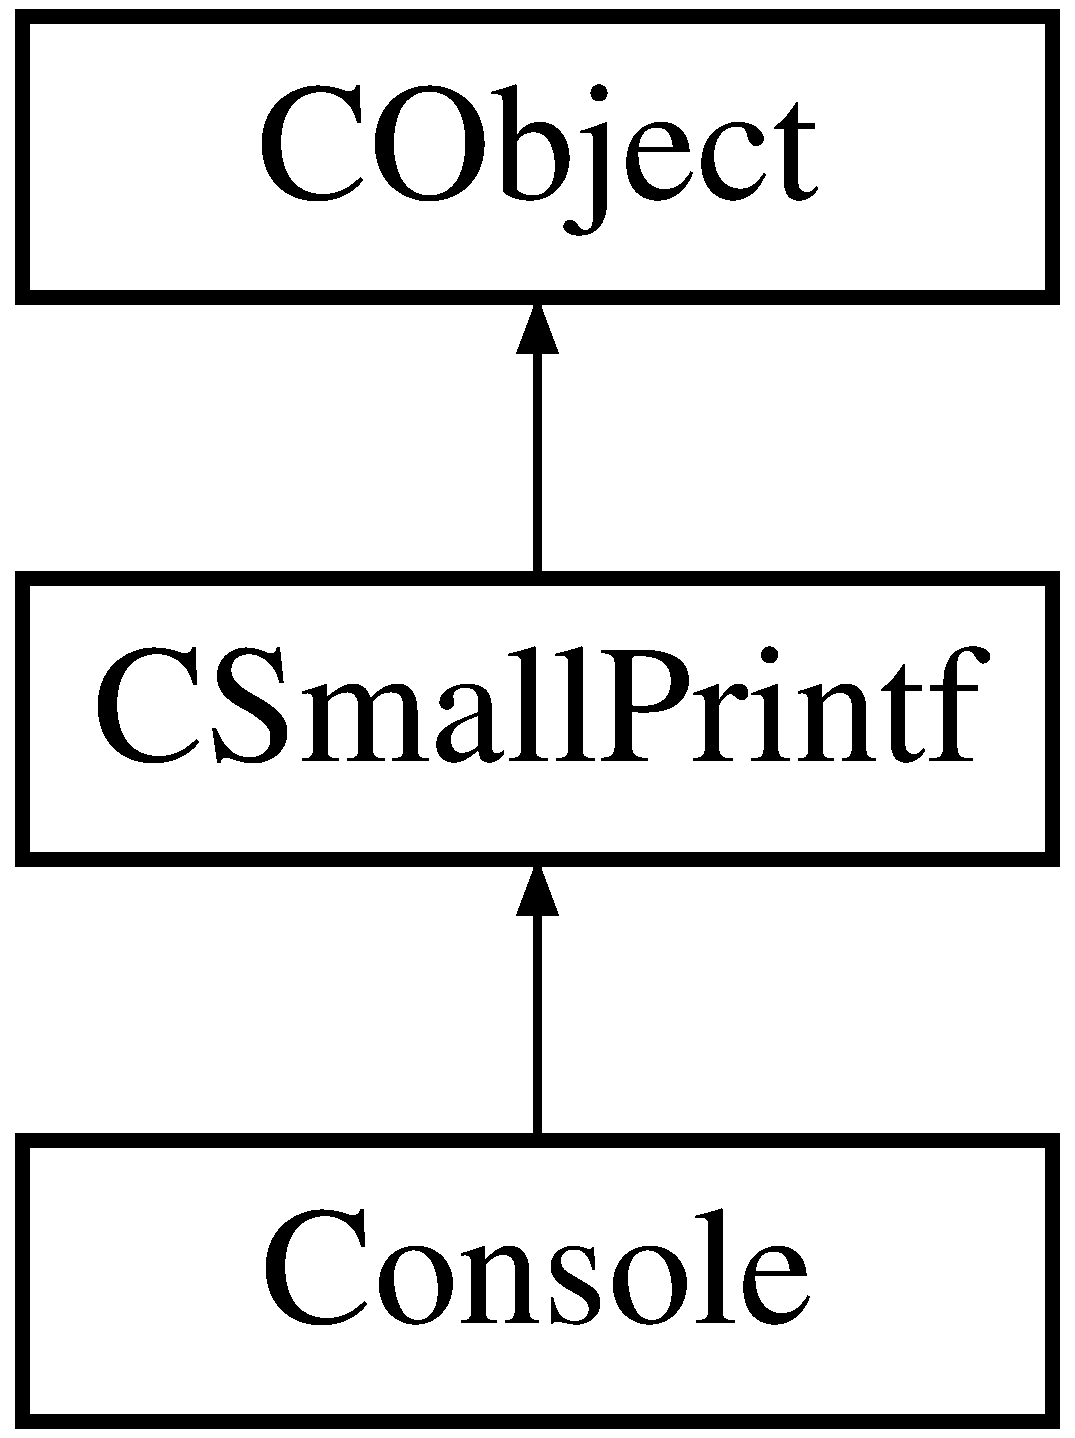
\includegraphics[height=3.000000cm]{class_console}
\end{center}
\end{figure}
\subsection*{Public Member Functions}
\begin{DoxyCompactItemize}
\item 
\hyperlink{class_console_a8374ffffac8edeaa0775bdd1923bdc10}{Console} (\hyperlink{class_c_stream}{C\-Stream} \&io)
\item 
virtual bool \hyperlink{class_console_a855191be30cd0e1eeaea2d6ab7cda03b}{is\-Connected} ()
\item 
virtual void \hyperlink{class_console_a78bb22aa6e31673a5675986c9c5e3529}{echo} (bool set)
\item 
virtual void \hyperlink{class_console_a61f9d57ebeecfd8553f02a84b4939e69}{clear} ()
\item 
virtual int \hyperlink{class_console_a1427b8f1d904381c49188a1f8d8da083}{putchar} (int ch)
\item 
virtual int \hyperlink{class_console_a404cc62475ef74f818d9102bdde09584}{getchar} ()
\item 
virtual int \hyperlink{class_console_a0a229393c4d71b47cb68d30397d5de1e}{putstr} (L\-P\-C\-T\-S\-T\-R str)
\item 
virtual int \hyperlink{class_console_ab28b81a0b1e462ec0df65ba0a573921f}{getstr} (L\-P\-T\-S\-T\-R strbuf, size\-\_\-t size)
\item 
virtual int \hyperlink{class_console_a3ff57fe349e1335039230e14b9fc0cb1}{write} (const void $\ast$buf, int size)
\item 
virtual int \hyperlink{class_console_a10df5763117e36da9f029d1dfa9641be}{read} (void $\ast$buf, int size)
\item 
virtual void \hyperlink{class_console_ae80d540e36c5522b8653359e1e4d6839}{operator$>$$>$} (char \&ch)
\item 
virtual void \hyperlink{class_console_a33c9beff5456efdd13209b8321df1a74}{operator$>$$>$} (uint8\-\_\-t \&b)
\item 
virtual \hyperlink{class_console}{Console} \& \hyperlink{class_console_afc5355f4c4fee0a91c4ba5ae6647f07d}{operator$<$$<$} (T\-C\-H\-A\-R ch)
\item 
virtual \hyperlink{class_console}{Console} \& \hyperlink{class_console_aa05d7169f95dc3a36b11a291e35c84ae}{operator$<$$<$} (L\-P\-C\-T\-S\-T\-R str)
\item 
virtual \hyperlink{class_console}{Console} \& \hyperlink{class_console_a01e2cf3bdbb5ff14689a8858e12da5ad}{operator$<$$<$} (int val)
\item 
virtual \hyperlink{class_console}{Console} \& \hyperlink{class_console_adaabaa6205705e13193e472a4cf7f194}{operator$<$$<$} (float val)
\item 
virtual \hyperlink{class_console}{Console} \& \hyperlink{class_console_ab765a1b1954e26b2cb725dc49c35fdeb}{operator$<$$<$} (double val)
\item 
virtual \hyperlink{class_console}{Console} \& \hyperlink{class_console_a756e1e290f184491bf98dfaa1247fff7}{operator$<$$<$} (size\-\_\-t val)
\item 
virtual \hyperlink{class_console}{Console} \& \hyperlink{class_console_a1da129a9f12eff89f82fc694bdc59231}{operator$<$$<$} (uint16\-\_\-t val)
\item 
\hypertarget{class_console_ad2d3cf94e3a31436681cc0839b760a75}{virtual \hyperlink{class_console}{Console} \& {\bfseries operator$<$$<$} (uint32\-\_\-t val)}\label{class_console_ad2d3cf94e3a31436681cc0839b760a75}

\item 
virtual \hyperlink{class_console}{Console} \& \hyperlink{class_console_a0b13c2318c5e62763b679c190223de54}{operator$<$$<$} (uint8\-\_\-t val)
\item 
virtual \hyperlink{class_console}{Console} \& \hyperlink{class_console_aed5d1ad55ac69f1173f610d7c75793a6}{operator$<$$<$} (C\-O\-N\-S\-O\-L\-E\-\_\-\-C\-T\-R\-L\-\_\-\-T ctrl)
\item 
\hyperlink{class_c_stream}{C\-Stream} $\ast$ \hyperlink{class_console_ad4d21815c5cbc33e9015ba5babf5bf09}{i\-Stream} ()
\item 
\hyperlink{class_c_stream}{C\-Stream} $\ast$ \hyperlink{class_console_af6941f3b8ce87a9e53f58c5a74936d49}{o\-Stream} ()
\end{DoxyCompactItemize}


\subsection{Detailed Description}
The \hyperlink{class_console}{Console} class provides a lightweight input/output stream to console. 

\subsection{Constructor \& Destructor Documentation}
\hypertarget{class_console_a8374ffffac8edeaa0775bdd1923bdc10}{\index{Console@{Console}!Console@{Console}}
\index{Console@{Console}!Console@{Console}}
\subsubsection[{Console}]{\setlength{\rightskip}{0pt plus 5cm}Console\-::\-Console (
\begin{DoxyParamCaption}
\item[{{\bf C\-Stream} \&}]{io}
\end{DoxyParamCaption}
)}}\label{class_console_a8374ffffac8edeaa0775bdd1923bdc10}
Constructs a console object. 
\begin{DoxyParams}{Parameters}
{\em io} & is a \hyperlink{class_c_stream}{C\-Stream} object to provide the input/output stream.\\
\hline
\end{DoxyParams}

\begin{DoxyCode}
Example:
        \hyperlink{class_c_serial}{CSerial} cdc(USB);       \textcolor{comment}{// create an USB serial stream object.}
        \hyperlink{class_console}{Console} con(cdc);       \textcolor{comment}{// create a console by the USB stream.}

        \textcolor{keywordflow}{if} ( con.isConnected() ) \{
            con << \textcolor{stringliteral}{"Hello World"} << endl;
        \}
\end{DoxyCode}
 

\subsection{Member Function Documentation}
\hypertarget{class_console_a61f9d57ebeecfd8553f02a84b4939e69}{\index{Console@{Console}!clear@{clear}}
\index{clear@{clear}!Console@{Console}}
\subsubsection[{clear}]{\setlength{\rightskip}{0pt plus 5cm}virtual void Console\-::clear (
\begin{DoxyParamCaption}
{}
\end{DoxyParamCaption}
)\hspace{0.3cm}{\ttfamily [virtual]}}}\label{class_console_a61f9d57ebeecfd8553f02a84b4939e69}
Call the member function to clear the screen of console. \hypertarget{class_console_a78bb22aa6e31673a5675986c9c5e3529}{\index{Console@{Console}!echo@{echo}}
\index{echo@{echo}!Console@{Console}}
\subsubsection[{echo}]{\setlength{\rightskip}{0pt plus 5cm}virtual void Console\-::echo (
\begin{DoxyParamCaption}
\item[{bool}]{set}
\end{DoxyParamCaption}
)\hspace{0.3cm}{\ttfamily [virtual]}}}\label{class_console_a78bb22aa6e31673a5675986c9c5e3529}
Call the member function to enable or disable the echo. 
\begin{DoxyParams}{Parameters}
{\em set} & is a boolean value, set true to enable the echo. \\
\hline
\end{DoxyParams}
\hypertarget{class_console_a404cc62475ef74f818d9102bdde09584}{\index{Console@{Console}!getchar@{getchar}}
\index{getchar@{getchar}!Console@{Console}}
\subsubsection[{getchar}]{\setlength{\rightskip}{0pt plus 5cm}virtual int Console\-::getchar (
\begin{DoxyParamCaption}
{}
\end{DoxyParamCaption}
)\hspace{0.3cm}{\ttfamily [inline]}, {\ttfamily [virtual]}}}\label{class_console_a404cc62475ef74f818d9102bdde09584}
Call the member function to get a character from the serial stream of console. \begin{DoxyReturn}{Returns}
the received character. 
\end{DoxyReturn}
\hypertarget{class_console_ab28b81a0b1e462ec0df65ba0a573921f}{\index{Console@{Console}!getstr@{getstr}}
\index{getstr@{getstr}!Console@{Console}}
\subsubsection[{getstr}]{\setlength{\rightskip}{0pt plus 5cm}virtual int Console\-::getstr (
\begin{DoxyParamCaption}
\item[{L\-P\-T\-S\-T\-R}]{strbuf, }
\item[{size\-\_\-t}]{size}
\end{DoxyParamCaption}
)\hspace{0.3cm}{\ttfamily [virtual]}}}\label{class_console_ab28b81a0b1e462ec0df65ba0a573921f}
Call the member function to get a string from the serial stream of console. 
\begin{DoxyParams}[1]{Parameters}
\mbox{\tt out}  & {\em strbuf} & is a string pointer where the string stored. \\
\hline
\mbox{\tt in}  & {\em size} & is a size\-\_\-t to represent the size of strbuf to be read. \\
\hline
\end{DoxyParams}
\begin{DoxyReturn}{Returns}
the how many characters received. 
\end{DoxyReturn}
\hypertarget{class_console_a855191be30cd0e1eeaea2d6ab7cda03b}{\index{Console@{Console}!is\-Connected@{is\-Connected}}
\index{is\-Connected@{is\-Connected}!Console@{Console}}
\subsubsection[{is\-Connected}]{\setlength{\rightskip}{0pt plus 5cm}virtual bool Console\-::is\-Connected (
\begin{DoxyParamCaption}
{}
\end{DoxyParamCaption}
)\hspace{0.3cm}{\ttfamily [virtual]}}}\label{class_console_a855191be30cd0e1eeaea2d6ab7cda03b}
Call the member function to check the stream is ready to read (or write).


\begin{DoxyCode}
Example:
        \hyperlink{class_c_serial}{CSerial} cdc(USB);       \textcolor{comment}{// create an USB serial stream object.}
        \hyperlink{class_console}{Console} con(cdc);       \textcolor{comment}{// create a console by the USB stream.}

        \textcolor{keywordflow}{if} ( con.isConnected() ) \{
            con << \textcolor{stringliteral}{"Hello World"} << endl;
        \}
\end{DoxyCode}
 \hypertarget{class_console_ad4d21815c5cbc33e9015ba5babf5bf09}{\index{Console@{Console}!i\-Stream@{i\-Stream}}
\index{i\-Stream@{i\-Stream}!Console@{Console}}
\subsubsection[{i\-Stream}]{\setlength{\rightskip}{0pt plus 5cm}{\bf C\-Stream}$\ast$ Console\-::i\-Stream (
\begin{DoxyParamCaption}
{}
\end{DoxyParamCaption}
)\hspace{0.3cm}{\ttfamily [inline]}}}\label{class_console_ad4d21815c5cbc33e9015ba5babf5bf09}
Call the member function to retrieve the input stream. \begin{DoxyReturn}{Returns}
a \hyperlink{class_c_stream}{C\-Stream} object for input. 
\end{DoxyReturn}
\hypertarget{class_console_afc5355f4c4fee0a91c4ba5ae6647f07d}{\index{Console@{Console}!operator$<$$<$@{operator$<$$<$}}
\index{operator$<$$<$@{operator$<$$<$}!Console@{Console}}
\subsubsection[{operator$<$$<$}]{\setlength{\rightskip}{0pt plus 5cm}virtual {\bf Console}\& Console\-::operator$<$$<$ (
\begin{DoxyParamCaption}
\item[{T\-C\-H\-A\-R}]{ch}
\end{DoxyParamCaption}
)\hspace{0.3cm}{\ttfamily [virtual]}}}\label{class_console_afc5355f4c4fee0a91c4ba5ae6647f07d}
A shorthand for write a character to console. \begin{DoxyReturn}{Returns}
$\ast$this.
\end{DoxyReturn}

\begin{DoxyCode}
Example:
        con << \textcolor{charliteral}{'?'} << \textcolor{stringliteral}{"Whate is it this year? "} << 2012 << endl;
\end{DoxyCode}
 \hypertarget{class_console_aa05d7169f95dc3a36b11a291e35c84ae}{\index{Console@{Console}!operator$<$$<$@{operator$<$$<$}}
\index{operator$<$$<$@{operator$<$$<$}!Console@{Console}}
\subsubsection[{operator$<$$<$}]{\setlength{\rightskip}{0pt plus 5cm}virtual {\bf Console}\& Console\-::operator$<$$<$ (
\begin{DoxyParamCaption}
\item[{L\-P\-C\-T\-S\-T\-R}]{str}
\end{DoxyParamCaption}
)\hspace{0.3cm}{\ttfamily [virtual]}}}\label{class_console_aa05d7169f95dc3a36b11a291e35c84ae}
A shorthand for write a string to console. \begin{DoxyReturn}{Returns}
$\ast$this.
\end{DoxyReturn}

\begin{DoxyCode}
Example:
        con << \textcolor{charliteral}{'?'} << \textcolor{stringliteral}{"Whate is it this year? "} << 2012 << endl;
\end{DoxyCode}
 \hypertarget{class_console_a01e2cf3bdbb5ff14689a8858e12da5ad}{\index{Console@{Console}!operator$<$$<$@{operator$<$$<$}}
\index{operator$<$$<$@{operator$<$$<$}!Console@{Console}}
\subsubsection[{operator$<$$<$}]{\setlength{\rightskip}{0pt plus 5cm}virtual {\bf Console}\& Console\-::operator$<$$<$ (
\begin{DoxyParamCaption}
\item[{int}]{val}
\end{DoxyParamCaption}
)\hspace{0.3cm}{\ttfamily [inline]}, {\ttfamily [virtual]}}}\label{class_console_a01e2cf3bdbb5ff14689a8858e12da5ad}
A shorthand for write a integer value to console. \begin{DoxyReturn}{Returns}
$\ast$this.
\end{DoxyReturn}

\begin{DoxyCode}
Example:
        con << \textcolor{charliteral}{'?'} << \textcolor{stringliteral}{"Whate is it this year? "} << 2012 << endl;
\end{DoxyCode}
 \hypertarget{class_console_adaabaa6205705e13193e472a4cf7f194}{\index{Console@{Console}!operator$<$$<$@{operator$<$$<$}}
\index{operator$<$$<$@{operator$<$$<$}!Console@{Console}}
\subsubsection[{operator$<$$<$}]{\setlength{\rightskip}{0pt plus 5cm}virtual {\bf Console}\& Console\-::operator$<$$<$ (
\begin{DoxyParamCaption}
\item[{float}]{val}
\end{DoxyParamCaption}
)\hspace{0.3cm}{\ttfamily [inline]}, {\ttfamily [virtual]}}}\label{class_console_adaabaa6205705e13193e472a4cf7f194}
A shorthand for write a float value to console. \begin{DoxyReturn}{Returns}
$\ast$this. 
\end{DoxyReturn}
\hypertarget{class_console_ab765a1b1954e26b2cb725dc49c35fdeb}{\index{Console@{Console}!operator$<$$<$@{operator$<$$<$}}
\index{operator$<$$<$@{operator$<$$<$}!Console@{Console}}
\subsubsection[{operator$<$$<$}]{\setlength{\rightskip}{0pt plus 5cm}virtual {\bf Console}\& Console\-::operator$<$$<$ (
\begin{DoxyParamCaption}
\item[{double}]{val}
\end{DoxyParamCaption}
)\hspace{0.3cm}{\ttfamily [inline]}, {\ttfamily [virtual]}}}\label{class_console_ab765a1b1954e26b2cb725dc49c35fdeb}
A shorthand for write a double value to console. \begin{DoxyReturn}{Returns}
$\ast$this. 
\end{DoxyReturn}
\hypertarget{class_console_a756e1e290f184491bf98dfaa1247fff7}{\index{Console@{Console}!operator$<$$<$@{operator$<$$<$}}
\index{operator$<$$<$@{operator$<$$<$}!Console@{Console}}
\subsubsection[{operator$<$$<$}]{\setlength{\rightskip}{0pt plus 5cm}virtual {\bf Console}\& Console\-::operator$<$$<$ (
\begin{DoxyParamCaption}
\item[{size\-\_\-t}]{val}
\end{DoxyParamCaption}
)\hspace{0.3cm}{\ttfamily [inline]}, {\ttfamily [virtual]}}}\label{class_console_a756e1e290f184491bf98dfaa1247fff7}
A shorthand for write a size\-\_\-t value to console. \begin{DoxyReturn}{Returns}
$\ast$this; 
\end{DoxyReturn}
\hypertarget{class_console_a1da129a9f12eff89f82fc694bdc59231}{\index{Console@{Console}!operator$<$$<$@{operator$<$$<$}}
\index{operator$<$$<$@{operator$<$$<$}!Console@{Console}}
\subsubsection[{operator$<$$<$}]{\setlength{\rightskip}{0pt plus 5cm}virtual {\bf Console}\& Console\-::operator$<$$<$ (
\begin{DoxyParamCaption}
\item[{uint16\-\_\-t}]{val}
\end{DoxyParamCaption}
)\hspace{0.3cm}{\ttfamily [inline]}, {\ttfamily [virtual]}}}\label{class_console_a1da129a9f12eff89f82fc694bdc59231}
A shorthand for write a unsigned integer 16 bits value to console. \begin{DoxyReturn}{Returns}
$\ast$this. 
\end{DoxyReturn}
\hypertarget{class_console_a0b13c2318c5e62763b679c190223de54}{\index{Console@{Console}!operator$<$$<$@{operator$<$$<$}}
\index{operator$<$$<$@{operator$<$$<$}!Console@{Console}}
\subsubsection[{operator$<$$<$}]{\setlength{\rightskip}{0pt plus 5cm}virtual {\bf Console}\& Console\-::operator$<$$<$ (
\begin{DoxyParamCaption}
\item[{uint8\-\_\-t}]{val}
\end{DoxyParamCaption}
)\hspace{0.3cm}{\ttfamily [inline]}, {\ttfamily [virtual]}}}\label{class_console_a0b13c2318c5e62763b679c190223de54}
A shorthand for write a unsigned integer 8 bits value to console. \begin{DoxyReturn}{Returns}
$\ast$this. 
\end{DoxyReturn}
\hypertarget{class_console_aed5d1ad55ac69f1173f610d7c75793a6}{\index{Console@{Console}!operator$<$$<$@{operator$<$$<$}}
\index{operator$<$$<$@{operator$<$$<$}!Console@{Console}}
\subsubsection[{operator$<$$<$}]{\setlength{\rightskip}{0pt plus 5cm}virtual {\bf Console}\& Console\-::operator$<$$<$ (
\begin{DoxyParamCaption}
\item[{C\-O\-N\-S\-O\-L\-E\-\_\-\-C\-T\-R\-L\-\_\-\-T}]{ctrl}
\end{DoxyParamCaption}
)\hspace{0.3cm}{\ttfamily [virtual]}}}\label{class_console_aed5d1ad55ac69f1173f610d7c75793a6}
A shorthand for write a control operator to console. \begin{DoxyReturn}{Returns}
$\ast$this;
\end{DoxyReturn}

\begin{DoxyCode}
Example:
        con << \textcolor{charliteral}{'?'} << \textcolor{stringliteral}{"Whate is it this year? "} << 2012 << endl;
\end{DoxyCode}
 \hypertarget{class_console_ae80d540e36c5522b8653359e1e4d6839}{\index{Console@{Console}!operator$>$$>$@{operator$>$$>$}}
\index{operator$>$$>$@{operator$>$$>$}!Console@{Console}}
\subsubsection[{operator$>$$>$}]{\setlength{\rightskip}{0pt plus 5cm}virtual void Console\-::operator$>$$>$ (
\begin{DoxyParamCaption}
\item[{char \&}]{ch}
\end{DoxyParamCaption}
)\hspace{0.3cm}{\ttfamily [virtual]}}}\label{class_console_ae80d540e36c5522b8653359e1e4d6839}
A shorthand for read a character.


\begin{DoxyCode}
Examle:
        \textcolor{keywordtype}{char} c;
        con >> c;
\end{DoxyCode}
 \hypertarget{class_console_a33c9beff5456efdd13209b8321df1a74}{\index{Console@{Console}!operator$>$$>$@{operator$>$$>$}}
\index{operator$>$$>$@{operator$>$$>$}!Console@{Console}}
\subsubsection[{operator$>$$>$}]{\setlength{\rightskip}{0pt plus 5cm}virtual void Console\-::operator$>$$>$ (
\begin{DoxyParamCaption}
\item[{uint8\-\_\-t \&}]{b}
\end{DoxyParamCaption}
)\hspace{0.3cm}{\ttfamily [virtual]}}}\label{class_console_a33c9beff5456efdd13209b8321df1a74}
A shorthand for read a byte value.


\begin{DoxyCode}
Example:
        byte c;
        con >> c;
\end{DoxyCode}
 \hypertarget{class_console_af6941f3b8ce87a9e53f58c5a74936d49}{\index{Console@{Console}!o\-Stream@{o\-Stream}}
\index{o\-Stream@{o\-Stream}!Console@{Console}}
\subsubsection[{o\-Stream}]{\setlength{\rightskip}{0pt plus 5cm}{\bf C\-Stream}$\ast$ Console\-::o\-Stream (
\begin{DoxyParamCaption}
{}
\end{DoxyParamCaption}
)\hspace{0.3cm}{\ttfamily [inline]}}}\label{class_console_af6941f3b8ce87a9e53f58c5a74936d49}
Call the member function to retrieve the output stream. \begin{DoxyReturn}{Returns}
a C\-Strea object for output. 
\end{DoxyReturn}
\hypertarget{class_console_a1427b8f1d904381c49188a1f8d8da083}{\index{Console@{Console}!putchar@{putchar}}
\index{putchar@{putchar}!Console@{Console}}
\subsubsection[{putchar}]{\setlength{\rightskip}{0pt plus 5cm}virtual int Console\-::putchar (
\begin{DoxyParamCaption}
\item[{int}]{ch}
\end{DoxyParamCaption}
)\hspace{0.3cm}{\ttfamily [inline]}, {\ttfamily [virtual]}}}\label{class_console_a1427b8f1d904381c49188a1f8d8da083}
Call the member function to put a character to the serial stream of console. 
\begin{DoxyParams}{Parameters}
{\em ch} & is a integer value of character. \\
\hline
\end{DoxyParams}
\begin{DoxyReturn}{Returns}
the same value, if put a character successful; 
\end{DoxyReturn}
\hypertarget{class_console_a0a229393c4d71b47cb68d30397d5de1e}{\index{Console@{Console}!putstr@{putstr}}
\index{putstr@{putstr}!Console@{Console}}
\subsubsection[{putstr}]{\setlength{\rightskip}{0pt plus 5cm}virtual int Console\-::putstr (
\begin{DoxyParamCaption}
\item[{L\-P\-C\-T\-S\-T\-R}]{str}
\end{DoxyParamCaption}
)\hspace{0.3cm}{\ttfamily [virtual]}}}\label{class_console_a0a229393c4d71b47cb68d30397d5de1e}
Call the member function to put a string to console. 
\begin{DoxyParams}[1]{Parameters}
\mbox{\tt in}  & {\em str} & is a string pointer to be written. \\
\hline
\end{DoxyParams}
\begin{DoxyReturn}{Returns}
the how many character sent. 
\end{DoxyReturn}
\hypertarget{class_console_a10df5763117e36da9f029d1dfa9641be}{\index{Console@{Console}!read@{read}}
\index{read@{read}!Console@{Console}}
\subsubsection[{read}]{\setlength{\rightskip}{0pt plus 5cm}virtual int Console\-::read (
\begin{DoxyParamCaption}
\item[{void $\ast$}]{buf, }
\item[{int}]{size}
\end{DoxyParamCaption}
)\hspace{0.3cm}{\ttfamily [virtual]}}}\label{class_console_a10df5763117e36da9f029d1dfa9641be}
Call the member function to read a block buffer from the serial stream of console. 
\begin{DoxyParams}[1]{Parameters}
\mbox{\tt out}  & {\em buf} & is a pointer to a block data where the content read will be stored. \\
\hline
\mbox{\tt in}  & {\em size} & is integer value to represent the size of block to be read. \\
\hline
\end{DoxyParams}
\begin{DoxyReturn}{Returns}
the how many byte to be read. 
\end{DoxyReturn}
\hypertarget{class_console_a3ff57fe349e1335039230e14b9fc0cb1}{\index{Console@{Console}!write@{write}}
\index{write@{write}!Console@{Console}}
\subsubsection[{write}]{\setlength{\rightskip}{0pt plus 5cm}virtual int Console\-::write (
\begin{DoxyParamCaption}
\item[{const void $\ast$}]{buf, }
\item[{int}]{size}
\end{DoxyParamCaption}
)\hspace{0.3cm}{\ttfamily [virtual]}}}\label{class_console_a3ff57fe349e1335039230e14b9fc0cb1}
Call the member function to write a block buffer to the serial stream of console. 
\begin{DoxyParams}[1]{Parameters}
\mbox{\tt in}  & {\em buf} & is a pointer to a block data with the content to be written. \\
\hline
\mbox{\tt in}  & {\em size} & is a integer value to specified the size of block to write. \\
\hline
\end{DoxyParams}
\begin{DoxyReturn}{Returns}
the how many bytes to write. 
\end{DoxyReturn}


The documentation for this class was generated from the following file\-:\begin{DoxyCompactItemize}
\item 
console.\-h\end{DoxyCompactItemize}

\hypertarget{class_c_peripheral}{\section{C\-Peripheral Class Reference}
\label{class_c_peripheral}\index{C\-Peripheral@{C\-Peripheral}}
}


{\ttfamily \#include $<$peripheral.\-h$>$}

Inheritance diagram for C\-Peripheral\-:\begin{figure}[H]
\begin{center}
\leavevmode
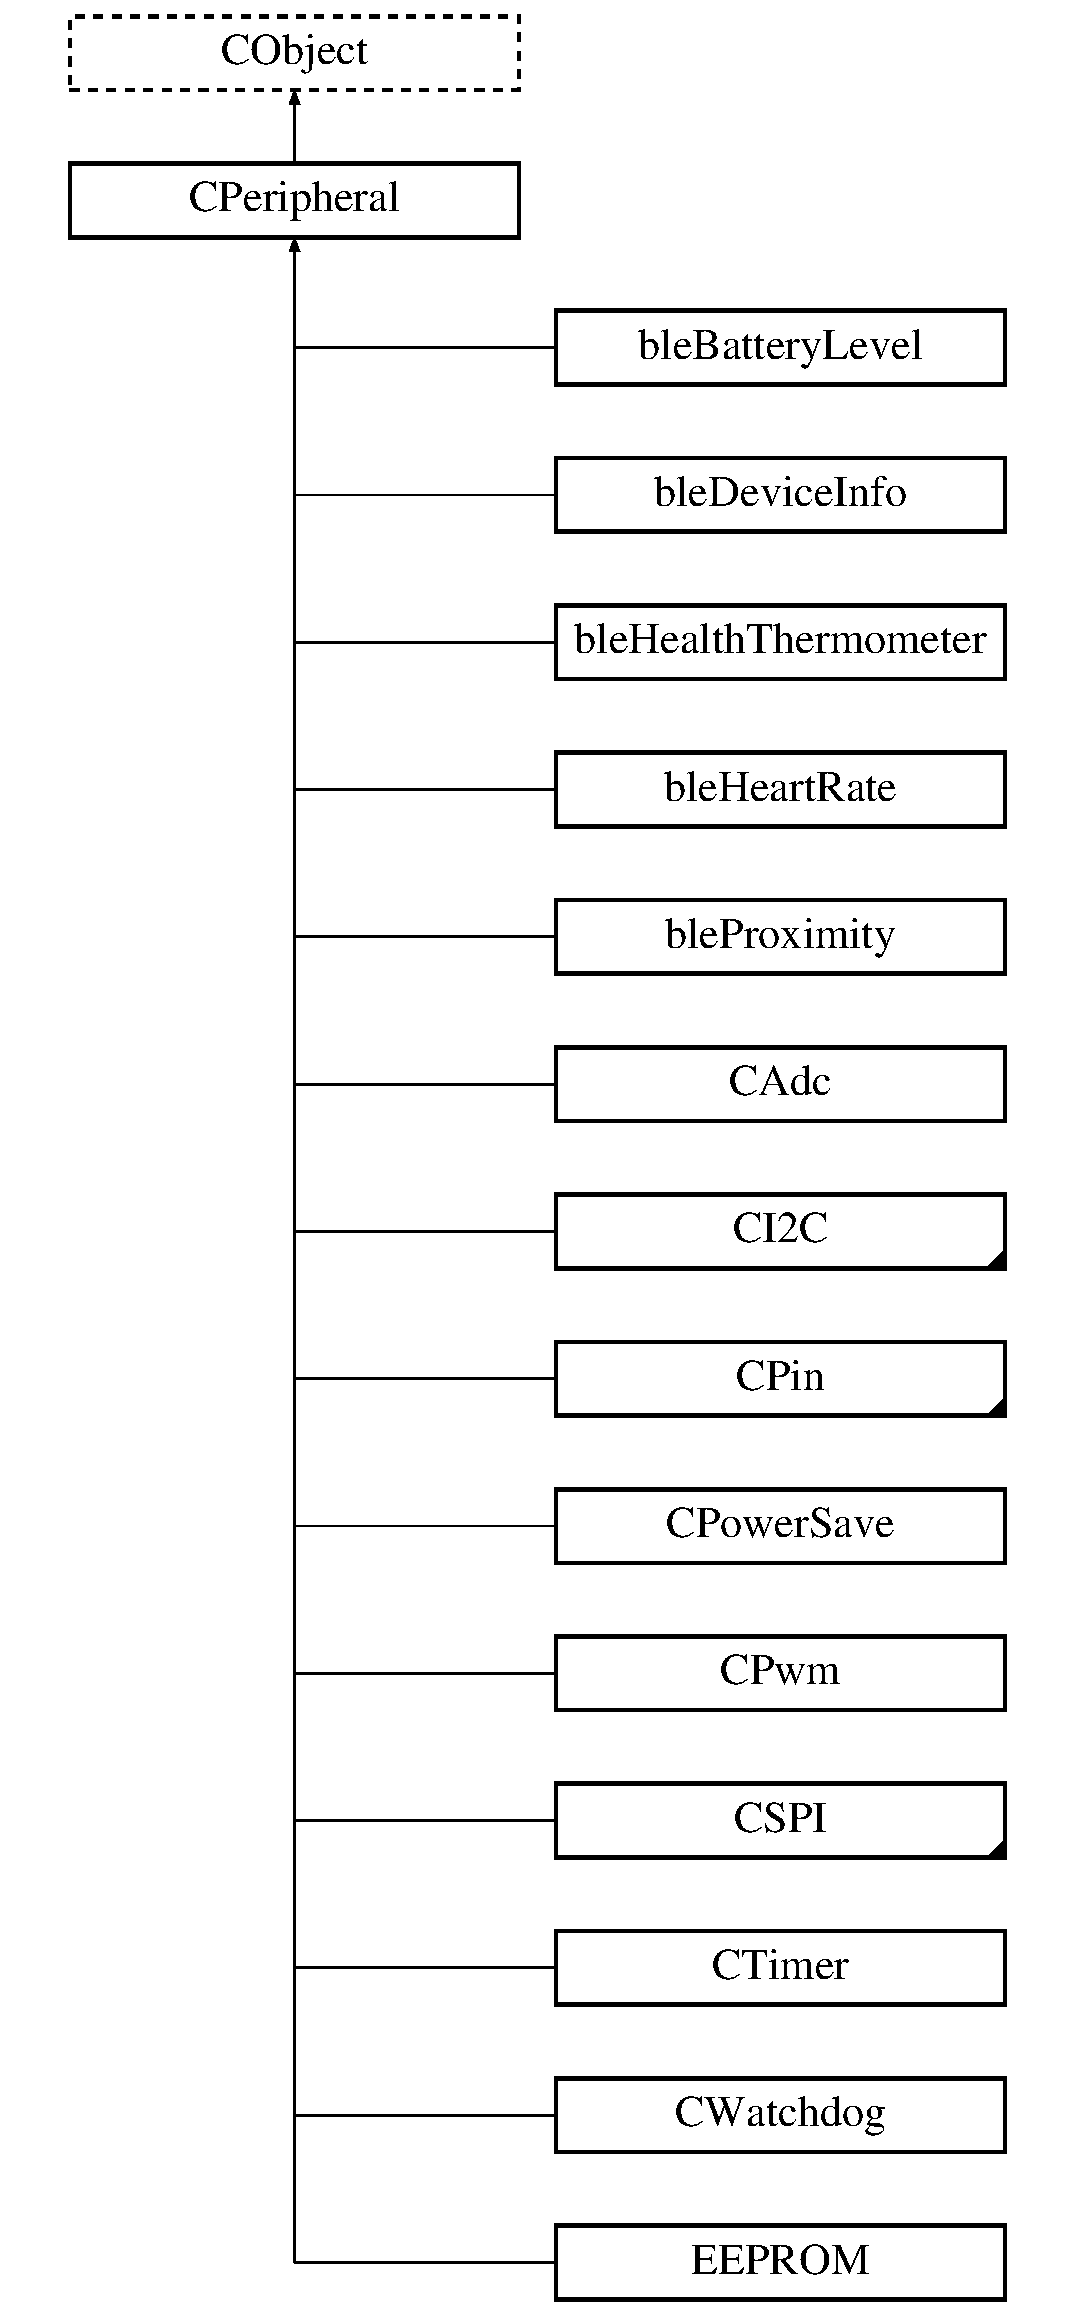
\includegraphics[height=12.000000cm]{d9/db6/class_c_peripheral}
\end{center}
\end{figure}
\subsection*{Additional Inherited Members}


The documentation for this class was generated from the following file\-:\begin{DoxyCompactItemize}
\item 
peripheral.\-h\end{DoxyCompactItemize}

\hypertarget{class_c_pin}{\section{C\-Pin Class Reference}
\label{class_c_pin}\index{C\-Pin@{C\-Pin}}
}


{\ttfamily \#include \char`\"{}class/pin.\-h\char`\"{}}

Inheritance diagram for C\-Pin\-:\begin{figure}[H]
\begin{center}
\leavevmode
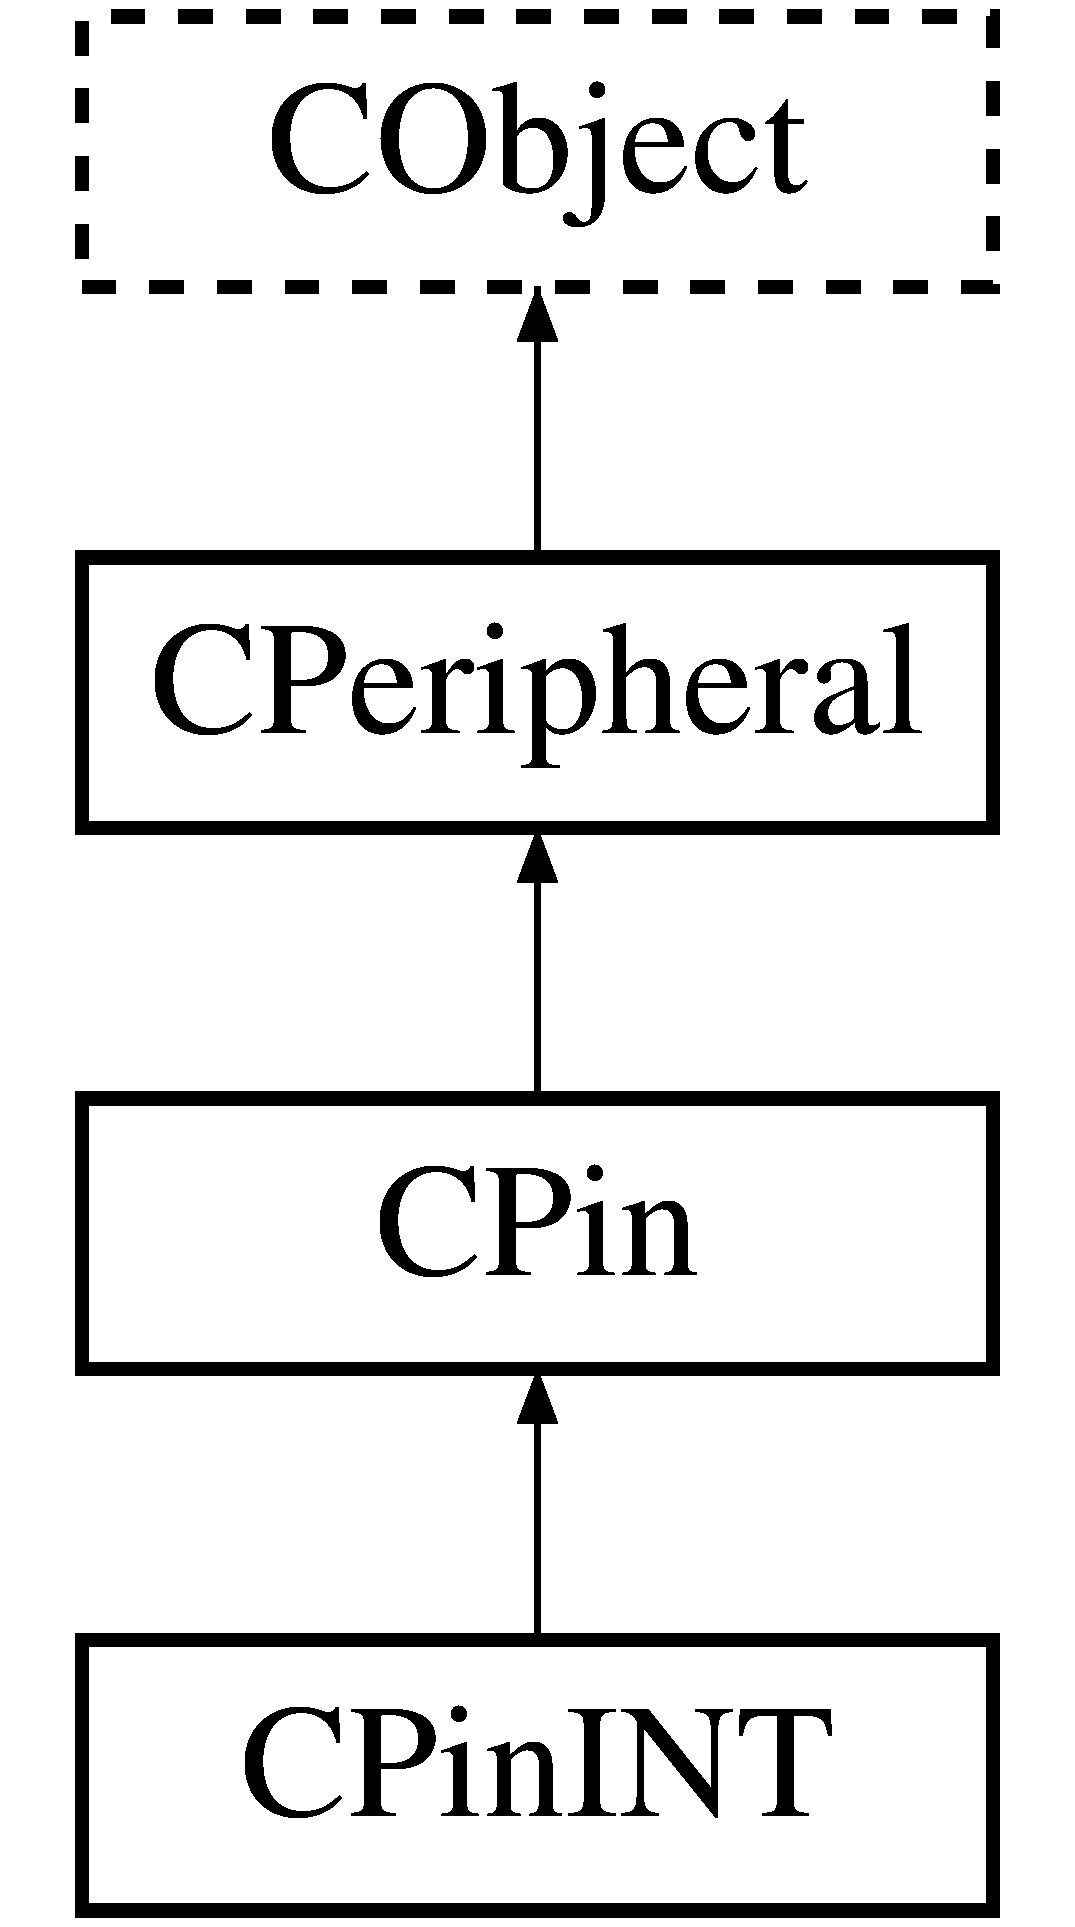
\includegraphics[height=4.000000cm]{d7/db9/class_c_pin}
\end{center}
\end{figure}
\subsection*{Public Member Functions}
\begin{DoxyCompactItemize}
\item 
\hyperlink{class_c_pin_a7338f2960b4d8992c43f3c6067742ded}{C\-Pin} (\hyperlink{group___enumerations_ga65a2241721e4acb573e0c3fe29ac432f}{P\-I\-N\-\_\-\-N\-A\-M\-E\-\_\-\-T} p)
\item 
virtual void \hyperlink{class_c_pin_a84cd9c4613a9b53f00e52c23b4eed050}{output} (\hyperlink{group___enumerations_gac16e35b75166ad7286b8bb78bd244ed2}{P\-I\-N\-\_\-\-O\-U\-T\-P\-U\-T\-\_\-\-M\-O\-D\-E\-\_\-\-T} mode=\hyperlink{group___enumerations_ggac16e35b75166ad7286b8bb78bd244ed2afd68b1a66f2a33ce77d4f6c7f8fc998a}{N\-O\-T\-\_\-\-O\-P\-E\-N}, \hyperlink{group___enumerations_ga6f24594071a026b31238ab8cb80d6a80}{P\-I\-N\-\_\-\-L\-E\-V\-E\-L\-\_\-\-T} def\-Value=\hyperlink{group___enumerations_gga6f24594071a026b31238ab8cb80d6a80a6a226f4143ca3b18999551694cdb72a8}{L\-O\-W})
\item 
virtual void \hyperlink{class_c_pin_a21aa5b473c1a3637a487c7724f8b9fcf}{input} (\hyperlink{group___enumerations_ga9f8f32709b482732d6e377ff26da36ef}{P\-I\-N\-\_\-\-I\-N\-P\-U\-T\-\_\-\-M\-O\-D\-E\-\_\-\-T} mode=\hyperlink{group___enumerations_gga9f8f32709b482732d6e377ff26da36efa781a7f23ae9b0dbdc6edfdcfd3be75df}{I\-N\-T\-E\-R\-N\-A\-L\-\_\-\-P\-U\-L\-L\-\_\-\-U\-P})
\item 
virtual void \hyperlink{class_c_pin_a1fc3486f4afea4de56ae677c20600551}{write} (\hyperlink{group___enumerations_ga6f24594071a026b31238ab8cb80d6a80}{P\-I\-N\-\_\-\-L\-E\-V\-E\-L\-\_\-\-T} val)
\item 
virtual \hyperlink{group___enumerations_ga6f24594071a026b31238ab8cb80d6a80}{P\-I\-N\-\_\-\-L\-E\-V\-E\-L\-\_\-\-T} \hyperlink{class_c_pin_a02060b0c9bbf0f75dead7bef1c75ce6b}{read} ()
\item 
virtual void \hyperlink{class_c_pin_a240de24c726724aeda90bfacf1d50cc5}{invert} ()
\item 
void \hyperlink{class_c_pin_a7d125bef83689d0f1db13b3f1acbd05e}{operator=} (\hyperlink{group___enumerations_ga6f24594071a026b31238ab8cb80d6a80}{P\-I\-N\-\_\-\-L\-E\-V\-E\-L\-\_\-\-T} val)
\item 
void \hyperlink{class_c_pin_a01428eca1b98e2e194bd0848b3eb8904}{operator=} (\hyperlink{class_c_pin}{C\-Pin} \&pin)
\item 
\hyperlink{class_c_pin_a9037649d1e88192f5fde46b810c71299}{operator P\-I\-N\-\_\-\-L\-E\-V\-E\-L\-\_\-\-T} ()
\item 
\hyperlink{group___enumerations_ga6f24594071a026b31238ab8cb80d6a80}{P\-I\-N\-\_\-\-L\-E\-V\-E\-L\-\_\-\-T} \hyperlink{class_c_pin_a5ec08fca85a5f9472e82588a6a895b8f}{operator!} ()
\item 
bool \hyperlink{class_c_pin_ae9f57493334eeb6e69a77a0cf4e50f95}{operator==} (\hyperlink{group___enumerations_ga6f24594071a026b31238ab8cb80d6a80}{P\-I\-N\-\_\-\-L\-E\-V\-E\-L\-\_\-\-T} val)
\item 
bool \hyperlink{class_c_pin_aae98a7d34d72ccc58b6d799f7ad2e12e}{operator!=} (\hyperlink{group___enumerations_ga6f24594071a026b31238ab8cb80d6a80}{P\-I\-N\-\_\-\-L\-E\-V\-E\-L\-\_\-\-T} val)
\item 
\hyperlink{group___enumerations_ga65a2241721e4acb573e0c3fe29ac432f}{P\-I\-N\-\_\-\-N\-A\-M\-E\-\_\-\-T} \hyperlink{class_c_pin_a5e6cdf81b6a8869e3c1e78dffb6ddca5}{name} ()
\end{DoxyCompactItemize}


\subsection{Detailed Description}
Pin define class 

\subsection{Constructor \& Destructor Documentation}
\hypertarget{class_c_pin_a7338f2960b4d8992c43f3c6067742ded}{\index{C\-Pin@{C\-Pin}!C\-Pin@{C\-Pin}}
\index{C\-Pin@{C\-Pin}!CPin@{C\-Pin}}
\subsubsection[{C\-Pin}]{\setlength{\rightskip}{0pt plus 5cm}C\-Pin\-::\-C\-Pin (
\begin{DoxyParamCaption}
\item[{{\bf P\-I\-N\-\_\-\-N\-A\-M\-E\-\_\-\-T}}]{p}
\end{DoxyParamCaption}
)}}\label{class_c_pin_a7338f2960b4d8992c43f3c6067742ded}
Constructs a \hyperlink{class_c_pin}{C\-Pin} object to connect to the specified pin. 
\begin{DoxyParams}{Parameters}
{\em p} & is a P\-I\-N\-\_\-\-N\-A\-M\-E\-\_\-\-T enumeration to a pin of peripheral.\\
\hline
\end{DoxyParams}

\begin{DoxyCode}
Example:
        \hyperlink{class_c_pin}{CPin} key(\hyperlink{group___enumerations_gga65a2241721e4acb573e0c3fe29ac432fa19b235491a16a3e7f91872f46a33a4a6}{P21});      \textcolor{comment}{// Create a key object to connect to pin 21.}
        key.input();        \textcolor{comment}{// set the key object as a input.}

        \textcolor{keywordflow}{if} ( key==\hyperlink{group___enumerations_gga6f24594071a026b31238ab8cb80d6a80a6a226f4143ca3b18999551694cdb72a8}{LOW} ) \{   \textcolor{comment}{// check the pin level}
        ...
        \}
\end{DoxyCode}
 

\subsection{Member Function Documentation}
\hypertarget{class_c_pin_a84cd9c4613a9b53f00e52c23b4eed050}{\index{C\-Pin@{C\-Pin}!output@{output}}
\index{output@{output}!CPin@{C\-Pin}}
\subsubsection[{output}]{\setlength{\rightskip}{0pt plus 5cm}virtual void C\-Pin\-::output (
\begin{DoxyParamCaption}
\item[{{\bf P\-I\-N\-\_\-\-O\-U\-T\-P\-U\-T\-\_\-\-M\-O\-D\-E\-\_\-\-T}}]{mode = {\ttfamily {\bf N\-O\-T\-\_\-\-O\-P\-E\-N}}, }
\item[{{\bf P\-I\-N\-\_\-\-L\-E\-V\-E\-L\-\_\-\-T}}]{def\-Value = {\ttfamily {\bf L\-O\-W}}}
\end{DoxyParamCaption}
)\hspace{0.3cm}{\ttfamily [virtual]}}}\label{class_c_pin_a84cd9c4613a9b53f00e52c23b4eed050}
Set the pin as an output pin. 
\begin{DoxyCode}
\hyperlink{class_c_pin}{CPin} myPin(\hyperlink{group___enumerations_gga65a2241721e4acb573e0c3fe29ac432fa61f13c350e3003e8df7d8001bb015b19}{P19});
myPin.output();     \textcolor{comment}{// set the P19 as an output pin. (use the default NOT\_OPEN and LOW level output)}
myPin = \hyperlink{group___enumerations_gga6f24594071a026b31238ab8cb80d6a80a0c3a1dacf94061154b3ee354359c5893}{HIGH};       \textcolor{comment}{// set P19 to HIGH (use the operator '=')}
myPin.write(\hyperlink{group___enumerations_gga6f24594071a026b31238ab8cb80d6a80a6a226f4143ca3b18999551694cdb72a8}{LOW});   \textcolor{comment}{// set P19 to LOW  (use the write() member)}
\end{DoxyCode}
 
\begin{DoxyParams}{Parameters}
{\em mode} & is a P\-I\-N\-\_\-\-O\-U\-T\-\_\-\-M\-O\-D\-E\-\_\-\-T enumeration to indicate the output mode. \\
\hline
{\em def\-Value} & is a P\-I\-N\-\_\-\-L\-E\-V\-E\-L\-\_\-\-T enumeration to set the default level for the output pin. \\
\hline
\end{DoxyParams}
\hypertarget{class_c_pin_a21aa5b473c1a3637a487c7724f8b9fcf}{\index{C\-Pin@{C\-Pin}!input@{input}}
\index{input@{input}!CPin@{C\-Pin}}
\subsubsection[{input}]{\setlength{\rightskip}{0pt plus 5cm}virtual void C\-Pin\-::input (
\begin{DoxyParamCaption}
\item[{{\bf P\-I\-N\-\_\-\-I\-N\-P\-U\-T\-\_\-\-M\-O\-D\-E\-\_\-\-T}}]{mode = {\ttfamily {\bf I\-N\-T\-E\-R\-N\-A\-L\-\_\-\-P\-U\-L\-L\-\_\-\-U\-P}}}
\end{DoxyParamCaption}
)\hspace{0.3cm}{\ttfamily [virtual]}}}\label{class_c_pin_a21aa5b473c1a3637a487c7724f8b9fcf}
Set as an input pin 
\begin{DoxyCode}
\hyperlink{group___enumerations_ga6f24594071a026b31238ab8cb80d6a80}{PIN\_LEVEL\_T} level;
\hyperlink{class_c_pin}{CPin} myPin(\hyperlink{group___enumerations_gga65a2241721e4acb573e0c3fe29ac432fa61f13c350e3003e8df7d8001bb015b19}{P19});
myPin.input();      \textcolor{comment}{// Set the P19 as an input pin. (with default INTERNAL\_PULL\_UP feature)}
\textcolor{keywordflow}{if} ( myPin==\hyperlink{group___enumerations_gga6f24594071a026b31238ab8cb80d6a80a0c3a1dacf94061154b3ee354359c5893}{HIGH} ) \{    \textcolor{comment}{// Read a pin level from myPin. (use the operator '==')}
        ...
\}
level = myPin;      \textcolor{comment}{// Read a pin level from myPin. (use the operator '=')}
level = myPin.read();\textcolor{comment}{// Read a pin level from myPin. (use the read() member)}
\end{DoxyCode}
 
\begin{DoxyParams}{Parameters}
{\em mode} & is a P\-I\-N\-\_\-\-I\-N\-P\-U\-T\-\_\-\-M\-O\-D\-E\-\_\-\-T enumeration to indicat the input mode. \\
\hline
\end{DoxyParams}
\hypertarget{class_c_pin_a1fc3486f4afea4de56ae677c20600551}{\index{C\-Pin@{C\-Pin}!write@{write}}
\index{write@{write}!CPin@{C\-Pin}}
\subsubsection[{write}]{\setlength{\rightskip}{0pt plus 5cm}virtual void C\-Pin\-::write (
\begin{DoxyParamCaption}
\item[{{\bf P\-I\-N\-\_\-\-L\-E\-V\-E\-L\-\_\-\-T}}]{val}
\end{DoxyParamCaption}
)\hspace{0.3cm}{\ttfamily [virtual]}}}\label{class_c_pin_a1fc3486f4afea4de56ae677c20600551}
Write a Pin Level to the output pin. 
\begin{DoxyParams}{Parameters}
{\em val} & is a P\-I\-N\-\_\-\-L\-E\-V\-E\-L\-\_\-\-T enumeration to write to the output pin. \\
\hline
\end{DoxyParams}
\begin{DoxySeeAlso}{See Also}
\hyperlink{class_c_pin_a84cd9c4613a9b53f00e52c23b4eed050}{output} 
\end{DoxySeeAlso}
\hypertarget{class_c_pin_a02060b0c9bbf0f75dead7bef1c75ce6b}{\index{C\-Pin@{C\-Pin}!read@{read}}
\index{read@{read}!CPin@{C\-Pin}}
\subsubsection[{read}]{\setlength{\rightskip}{0pt plus 5cm}virtual {\bf P\-I\-N\-\_\-\-L\-E\-V\-E\-L\-\_\-\-T} C\-Pin\-::read (
\begin{DoxyParamCaption}
{}
\end{DoxyParamCaption}
)\hspace{0.3cm}{\ttfamily [virtual]}}}\label{class_c_pin_a02060b0c9bbf0f75dead7bef1c75ce6b}
Read a Pin Level from the input pin. \begin{DoxyReturn}{Returns}
P\-I\-N\-\_\-\-L\-E\-V\-E\-L\-\_\-\-T is H\-I\-G\-H (or L\-O\-W) enumeration. 
\end{DoxyReturn}
\begin{DoxySeeAlso}{See Also}
\hyperlink{class_c_pin_a21aa5b473c1a3637a487c7724f8b9fcf}{input} 
\end{DoxySeeAlso}
\hypertarget{class_c_pin_a240de24c726724aeda90bfacf1d50cc5}{\index{C\-Pin@{C\-Pin}!invert@{invert}}
\index{invert@{invert}!CPin@{C\-Pin}}
\subsubsection[{invert}]{\setlength{\rightskip}{0pt plus 5cm}virtual void C\-Pin\-::invert (
\begin{DoxyParamCaption}
{}
\end{DoxyParamCaption}
)\hspace{0.3cm}{\ttfamily [virtual]}}}\label{class_c_pin_a240de24c726724aeda90bfacf1d50cc5}
Invert an output pin. 
\begin{DoxyCode}
\hyperlink{class_c_pin}{CPin} myPin(\hyperlink{group___enumerations_gga65a2241721e4acb573e0c3fe29ac432fa61f13c350e3003e8df7d8001bb015b19}{P19});
myPin.output();

\textcolor{keywordflow}{while}(1) \{
        myPin.invert(); \textcolor{comment}{// Invert the output pin level. (use the invert() member)}
\textcolor{comment}{//   myPin = !myPin; // Invert the output pin level. (use the '!' operator)}
        sleep(100);
\}
\end{DoxyCode}
 \hypertarget{class_c_pin_a7d125bef83689d0f1db13b3f1acbd05e}{\index{C\-Pin@{C\-Pin}!operator=@{operator=}}
\index{operator=@{operator=}!CPin@{C\-Pin}}
\subsubsection[{operator=}]{\setlength{\rightskip}{0pt plus 5cm}void C\-Pin\-::operator= (
\begin{DoxyParamCaption}
\item[{{\bf P\-I\-N\-\_\-\-L\-E\-V\-E\-L\-\_\-\-T}}]{val}
\end{DoxyParamCaption}
)\hspace{0.3cm}{\ttfamily [inline]}}}\label{class_c_pin_a7d125bef83689d0f1db13b3f1acbd05e}
\hypertarget{class_c_pin_a01428eca1b98e2e194bd0848b3eb8904}{\index{C\-Pin@{C\-Pin}!operator=@{operator=}}
\index{operator=@{operator=}!CPin@{C\-Pin}}
\subsubsection[{operator=}]{\setlength{\rightskip}{0pt plus 5cm}void C\-Pin\-::operator= (
\begin{DoxyParamCaption}
\item[{{\bf C\-Pin} \&}]{pin}
\end{DoxyParamCaption}
)\hspace{0.3cm}{\ttfamily [inline]}}}\label{class_c_pin_a01428eca1b98e2e194bd0848b3eb8904}
\hypertarget{class_c_pin_a9037649d1e88192f5fde46b810c71299}{\index{C\-Pin@{C\-Pin}!operator P\-I\-N\-\_\-\-L\-E\-V\-E\-L\-\_\-\-T@{operator P\-I\-N\-\_\-\-L\-E\-V\-E\-L\-\_\-\-T}}
\index{operator P\-I\-N\-\_\-\-L\-E\-V\-E\-L\-\_\-\-T@{operator P\-I\-N\-\_\-\-L\-E\-V\-E\-L\-\_\-\-T}!CPin@{C\-Pin}}
\subsubsection[{operator P\-I\-N\-\_\-\-L\-E\-V\-E\-L\-\_\-\-T}]{\setlength{\rightskip}{0pt plus 5cm}C\-Pin\-::operator {\bf P\-I\-N\-\_\-\-L\-E\-V\-E\-L\-\_\-\-T} (
\begin{DoxyParamCaption}
{}
\end{DoxyParamCaption}
)\hspace{0.3cm}{\ttfamily [inline]}}}\label{class_c_pin_a9037649d1e88192f5fde46b810c71299}
\hypertarget{class_c_pin_a5ec08fca85a5f9472e82588a6a895b8f}{\index{C\-Pin@{C\-Pin}!operator!@{operator!}}
\index{operator!@{operator!}!CPin@{C\-Pin}}
\subsubsection[{operator!}]{\setlength{\rightskip}{0pt plus 5cm}{\bf P\-I\-N\-\_\-\-L\-E\-V\-E\-L\-\_\-\-T} C\-Pin\-::operator! (
\begin{DoxyParamCaption}
{}
\end{DoxyParamCaption}
)\hspace{0.3cm}{\ttfamily [inline]}}}\label{class_c_pin_a5ec08fca85a5f9472e82588a6a895b8f}
\hypertarget{class_c_pin_ae9f57493334eeb6e69a77a0cf4e50f95}{\index{C\-Pin@{C\-Pin}!operator==@{operator==}}
\index{operator==@{operator==}!CPin@{C\-Pin}}
\subsubsection[{operator==}]{\setlength{\rightskip}{0pt plus 5cm}bool C\-Pin\-::operator== (
\begin{DoxyParamCaption}
\item[{{\bf P\-I\-N\-\_\-\-L\-E\-V\-E\-L\-\_\-\-T}}]{val}
\end{DoxyParamCaption}
)\hspace{0.3cm}{\ttfamily [inline]}}}\label{class_c_pin_ae9f57493334eeb6e69a77a0cf4e50f95}
\hypertarget{class_c_pin_aae98a7d34d72ccc58b6d799f7ad2e12e}{\index{C\-Pin@{C\-Pin}!operator!=@{operator!=}}
\index{operator!=@{operator!=}!CPin@{C\-Pin}}
\subsubsection[{operator!=}]{\setlength{\rightskip}{0pt plus 5cm}bool {\bf C\-Pin\-::operator!}= (
\begin{DoxyParamCaption}
\item[{{\bf P\-I\-N\-\_\-\-L\-E\-V\-E\-L\-\_\-\-T}}]{val}
\end{DoxyParamCaption}
)\hspace{0.3cm}{\ttfamily [inline]}}}\label{class_c_pin_aae98a7d34d72ccc58b6d799f7ad2e12e}
\hypertarget{class_c_pin_a5e6cdf81b6a8869e3c1e78dffb6ddca5}{\index{C\-Pin@{C\-Pin}!name@{name}}
\index{name@{name}!CPin@{C\-Pin}}
\subsubsection[{name}]{\setlength{\rightskip}{0pt plus 5cm}{\bf P\-I\-N\-\_\-\-N\-A\-M\-E\-\_\-\-T} C\-Pin\-::name (
\begin{DoxyParamCaption}
{}
\end{DoxyParamCaption}
)\hspace{0.3cm}{\ttfamily [inline]}}}\label{class_c_pin_a5e6cdf81b6a8869e3c1e78dffb6ddca5}
Call the \hyperlink{class_c_pin_a5e6cdf81b6a8869e3c1e78dffb6ddca5}{name()} member to retrieve the Pin Name of Object \begin{DoxyReturn}{Returns}
P\-I\-N\-\_\-\-N\-A\-M\-E\-\_\-\-T name 
\end{DoxyReturn}


The documentation for this class was generated from the following file\-:\begin{DoxyCompactItemize}
\item 
pin.\-h\end{DoxyCompactItemize}

\hypertarget{class_c_pin_i_n_t}{\section{C\-Pin\-I\-N\-T Class Reference}
\label{class_c_pin_i_n_t}\index{C\-Pin\-I\-N\-T@{C\-Pin\-I\-N\-T}}
}


{\ttfamily \#include $<$pinint.\-h$>$}

Inheritance diagram for C\-Pin\-I\-N\-T\-:\begin{figure}[H]
\begin{center}
\leavevmode
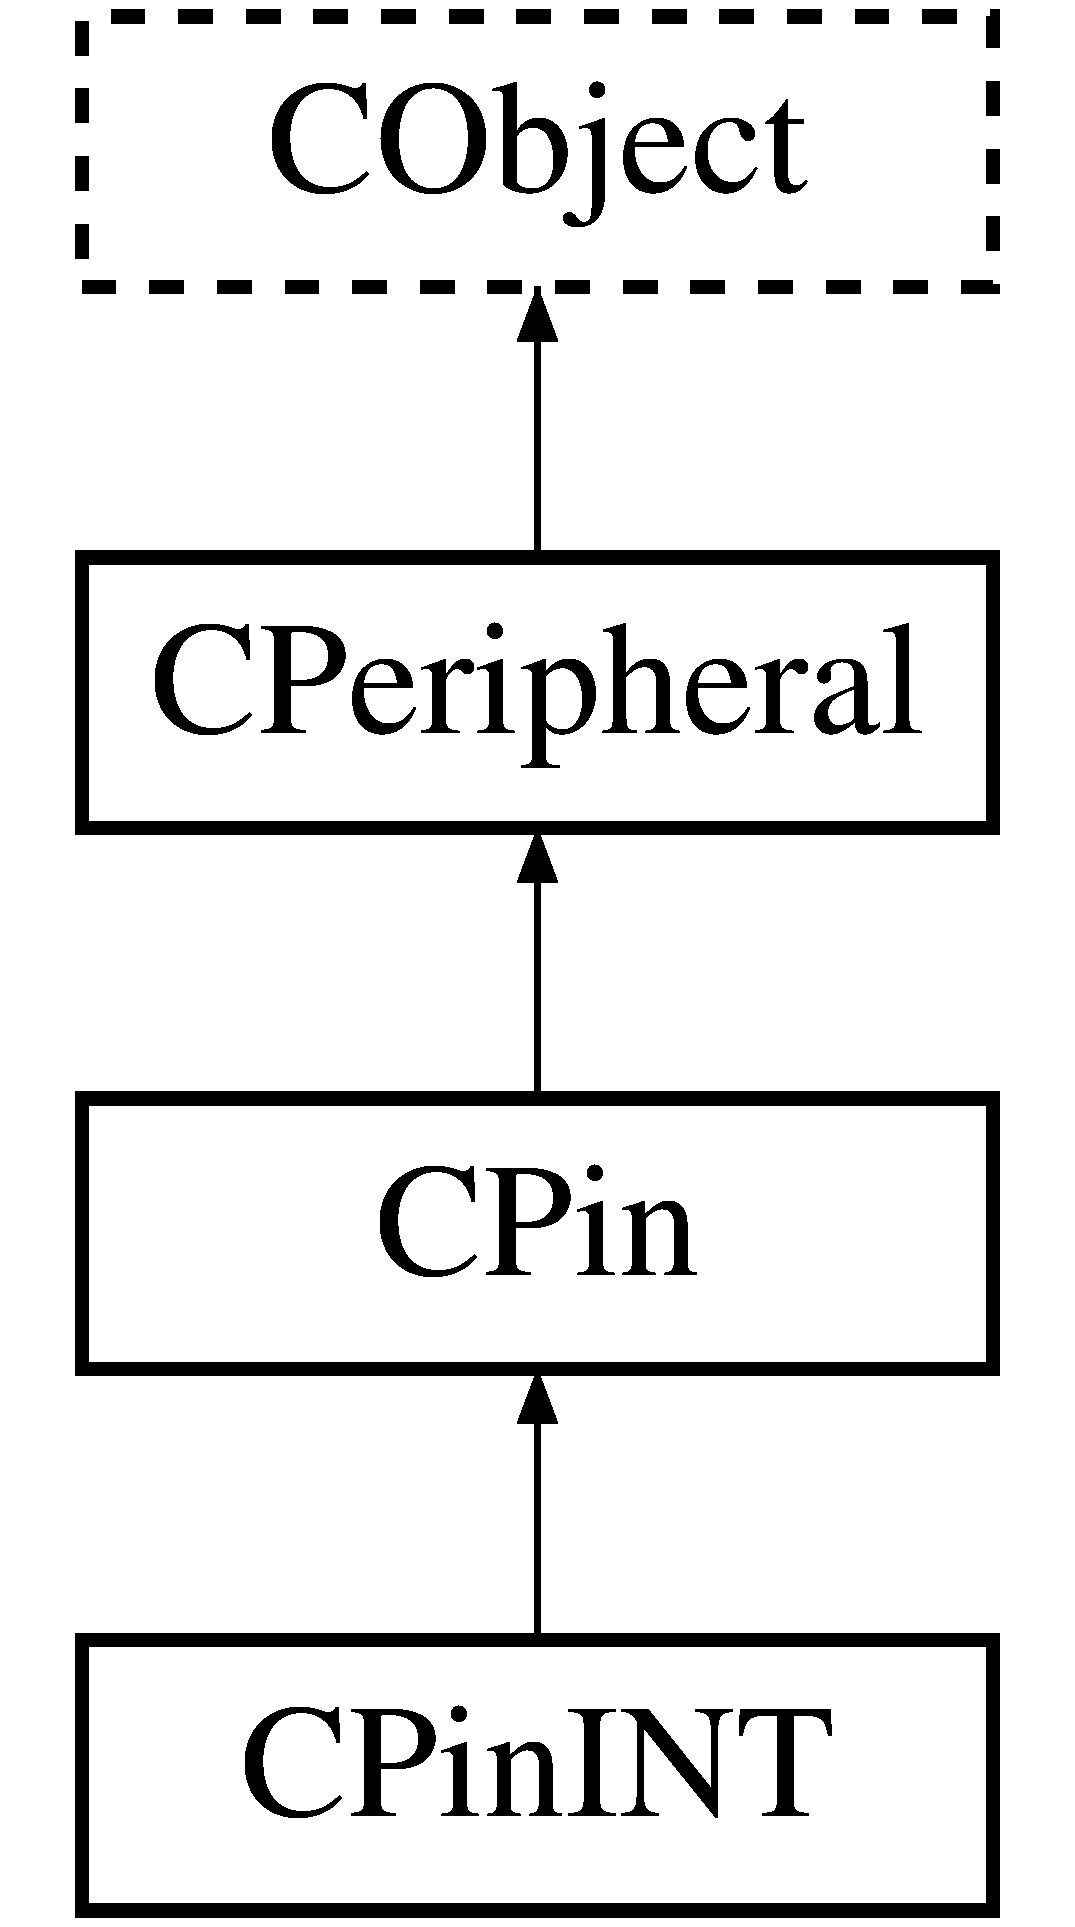
\includegraphics[height=4.000000cm]{db/d2c/class_c_pin_i_n_t}
\end{center}
\end{figure}
\subsection*{Public Member Functions}
\begin{DoxyCompactItemize}
\item 
\hyperlink{class_c_pin_i_n_t_a71f5452b1d99597b04082bf402f4ae59}{C\-Pin\-I\-N\-T} (\hyperlink{group___peripheral_ga65a2241721e4acb573e0c3fe29ac432f}{P\-I\-N\-\_\-\-N\-A\-M\-E\-\_\-\-T} pin, E\-D\-G\-E\-\_\-\-S\-T\-A\-T\-E\-\_\-\-T edge, \hyperlink{group___peripheral_gad5705547b72a4480dc714447b3bbfb64}{P\-I\-N\-\_\-\-I\-N\-P\-U\-T\-\_\-\-M\-O\-D\-E\-\_\-\-T} mode=\hyperlink{group___peripheral_gga16ce6180d8bb2eb23a7df8f8923ea581a781a7f23ae9b0dbdc6edfdcfd3be75df}{I\-N\-T\-E\-R\-N\-A\-L\-\_\-\-P\-U\-L\-L\-\_\-\-U\-P})
\item 
\hyperlink{class_c_pin_i_n_t_a48e6afdca1e70de51e292d1d3c4bafc5}{C\-Pin\-I\-N\-T} (\hyperlink{group___peripheral_ga65a2241721e4acb573e0c3fe29ac432f}{P\-I\-N\-\_\-\-N\-A\-M\-E\-\_\-\-T} pin, \hyperlink{group___peripheral_gac4a9005971c102914017b5e21ae23a19}{P\-I\-N\-\_\-\-L\-E\-V\-E\-L\-\_\-\-T} level, \hyperlink{group___peripheral_gad5705547b72a4480dc714447b3bbfb64}{P\-I\-N\-\_\-\-I\-N\-P\-U\-T\-\_\-\-M\-O\-D\-E\-\_\-\-T} mode=\hyperlink{group___peripheral_gga16ce6180d8bb2eb23a7df8f8923ea581a781a7f23ae9b0dbdc6edfdcfd3be75df}{I\-N\-T\-E\-R\-N\-A\-L\-\_\-\-P\-U\-L\-L\-\_\-\-U\-P})
\item 
virtual void \hyperlink{class_c_pin_i_n_t_a36d2301b10290741be6d3dd86dbc534b}{enable} ()
\item 
virtual void \hyperlink{class_c_pin_i_n_t_a08521d6d6892b7a80452bfce7db03e2b}{disable} ()
\item 
void \hyperlink{class_c_pin_i_n_t_a811526191ebf7ba17f0f51dea004d37b}{begin} ()
\item 
void \hyperlink{class_c_pin_i_n_t_a9f65ac4a7485b63e46b232f8d7ab385f}{end} ()
\item 
virtual bool \hyperlink{class_c_pin_i_n_t_a45e9fb4b6e6300e4c1c2ed6c13cfc062}{wait} (uint32\-\_\-t tm=M\-A\-X\-\_\-\-D\-E\-L\-A\-Y\-\_\-\-T\-I\-M\-E)
\item 
virtual void \hyperlink{class_c_pin_i_n_t_abe0ce7ac090423e11d460e75c8838128}{release} ()
\item 
void \hyperlink{class_c_pin_i_n_t_ae30634b8f9107d2ce4b6c3a52aeb380a}{as\-Weakup\-Source} ()
\item 
virtual \hyperlink{class_c_pin_i_n_t_ab75df389802ed381ac35726196ee15bb}{$\sim$\-C\-Pin\-I\-N\-T} ()
\end{DoxyCompactItemize}
\subsection*{Public Attributes}
\begin{DoxyCompactItemize}
\item 
\hyperlink{class_c_semaphore}{C\-Semaphore} \hyperlink{class_c_pin_i_n_t_a183f478d30ac65d5a3e85c7939db044e}{m\-\_\-sem\-Irq}
\item 
uint32\-\_\-t \hyperlink{class_c_pin_i_n_t_a53b3ac0896504d345f4b6093cb22f3f3}{m\-\_\-event}
\end{DoxyCompactItemize}
\subsection*{Protected Member Functions}
\begin{DoxyCompactItemize}
\item 
virtual void \hyperlink{class_c_pin_i_n_t_a762631f4e29ba2f09257af8892f8777e}{assign} (\hyperlink{group___peripheral_ga65a2241721e4acb573e0c3fe29ac432f}{P\-I\-N\-\_\-\-N\-A\-M\-E\-\_\-\-T} pin, \hyperlink{group___peripheral_gad5705547b72a4480dc714447b3bbfb64}{P\-I\-N\-\_\-\-I\-N\-P\-U\-T\-\_\-\-M\-O\-D\-E\-\_\-\-T} mode)
\end{DoxyCompactItemize}
\subsection*{Static Protected Member Functions}
\begin{DoxyCompactItemize}
\item 
static int \hyperlink{class_c_pin_i_n_t_ac638835b5fd1ca3f7c29af36677e2b0a}{get\-Free\-Channel} ()
\end{DoxyCompactItemize}
\subsection*{Protected Attributes}
\begin{DoxyCompactItemize}
\item 
int \hyperlink{class_c_pin_i_n_t_a563b913b2126f003c0e1e2f3400a2ed2}{m\-\_\-ch}
\end{DoxyCompactItemize}


\subsection{Constructor \& Destructor Documentation}
\hypertarget{class_c_pin_i_n_t_a71f5452b1d99597b04082bf402f4ae59}{\index{C\-Pin\-I\-N\-T@{C\-Pin\-I\-N\-T}!C\-Pin\-I\-N\-T@{C\-Pin\-I\-N\-T}}
\index{C\-Pin\-I\-N\-T@{C\-Pin\-I\-N\-T}!CPinINT@{C\-Pin\-I\-N\-T}}
\subsubsection[{C\-Pin\-I\-N\-T}]{\setlength{\rightskip}{0pt plus 5cm}C\-Pin\-I\-N\-T\-::\-C\-Pin\-I\-N\-T (
\begin{DoxyParamCaption}
\item[{{\bf P\-I\-N\-\_\-\-N\-A\-M\-E\-\_\-\-T}}]{pin, }
\item[{E\-D\-G\-E\-\_\-\-S\-T\-A\-T\-E\-\_\-\-T}]{edge, }
\item[{{\bf P\-I\-N\-\_\-\-I\-N\-P\-U\-T\-\_\-\-M\-O\-D\-E\-\_\-\-T}}]{mode = {\ttfamily {\bf I\-N\-T\-E\-R\-N\-A\-L\-\_\-\-P\-U\-L\-L\-\_\-\-U\-P}}}
\end{DoxyParamCaption}
)}}\label{class_c_pin_i_n_t_a71f5452b1d99597b04082bf402f4ae59}
\hypertarget{class_c_pin_i_n_t_a48e6afdca1e70de51e292d1d3c4bafc5}{\index{C\-Pin\-I\-N\-T@{C\-Pin\-I\-N\-T}!C\-Pin\-I\-N\-T@{C\-Pin\-I\-N\-T}}
\index{C\-Pin\-I\-N\-T@{C\-Pin\-I\-N\-T}!CPinINT@{C\-Pin\-I\-N\-T}}
\subsubsection[{C\-Pin\-I\-N\-T}]{\setlength{\rightskip}{0pt plus 5cm}C\-Pin\-I\-N\-T\-::\-C\-Pin\-I\-N\-T (
\begin{DoxyParamCaption}
\item[{{\bf P\-I\-N\-\_\-\-N\-A\-M\-E\-\_\-\-T}}]{pin, }
\item[{{\bf P\-I\-N\-\_\-\-L\-E\-V\-E\-L\-\_\-\-T}}]{level, }
\item[{{\bf P\-I\-N\-\_\-\-I\-N\-P\-U\-T\-\_\-\-M\-O\-D\-E\-\_\-\-T}}]{mode = {\ttfamily {\bf I\-N\-T\-E\-R\-N\-A\-L\-\_\-\-P\-U\-L\-L\-\_\-\-U\-P}}}
\end{DoxyParamCaption}
)}}\label{class_c_pin_i_n_t_a48e6afdca1e70de51e292d1d3c4bafc5}
\hypertarget{class_c_pin_i_n_t_ab75df389802ed381ac35726196ee15bb}{\index{C\-Pin\-I\-N\-T@{C\-Pin\-I\-N\-T}!$\sim$\-C\-Pin\-I\-N\-T@{$\sim$\-C\-Pin\-I\-N\-T}}
\index{$\sim$\-C\-Pin\-I\-N\-T@{$\sim$\-C\-Pin\-I\-N\-T}!CPinINT@{C\-Pin\-I\-N\-T}}
\subsubsection[{$\sim$\-C\-Pin\-I\-N\-T}]{\setlength{\rightskip}{0pt plus 5cm}virtual C\-Pin\-I\-N\-T\-::$\sim$\-C\-Pin\-I\-N\-T (
\begin{DoxyParamCaption}
{}
\end{DoxyParamCaption}
)\hspace{0.3cm}{\ttfamily [virtual]}}}\label{class_c_pin_i_n_t_ab75df389802ed381ac35726196ee15bb}


\subsection{Member Function Documentation}
\hypertarget{class_c_pin_i_n_t_a36d2301b10290741be6d3dd86dbc534b}{\index{C\-Pin\-I\-N\-T@{C\-Pin\-I\-N\-T}!enable@{enable}}
\index{enable@{enable}!CPinINT@{C\-Pin\-I\-N\-T}}
\subsubsection[{enable}]{\setlength{\rightskip}{0pt plus 5cm}virtual void C\-Pin\-I\-N\-T\-::enable (
\begin{DoxyParamCaption}
{}
\end{DoxyParamCaption}
)\hspace{0.3cm}{\ttfamily [virtual]}}}\label{class_c_pin_i_n_t_a36d2301b10290741be6d3dd86dbc534b}
\hypertarget{class_c_pin_i_n_t_a08521d6d6892b7a80452bfce7db03e2b}{\index{C\-Pin\-I\-N\-T@{C\-Pin\-I\-N\-T}!disable@{disable}}
\index{disable@{disable}!CPinINT@{C\-Pin\-I\-N\-T}}
\subsubsection[{disable}]{\setlength{\rightskip}{0pt plus 5cm}virtual void C\-Pin\-I\-N\-T\-::disable (
\begin{DoxyParamCaption}
{}
\end{DoxyParamCaption}
)\hspace{0.3cm}{\ttfamily [virtual]}}}\label{class_c_pin_i_n_t_a08521d6d6892b7a80452bfce7db03e2b}
\hypertarget{class_c_pin_i_n_t_a811526191ebf7ba17f0f51dea004d37b}{\index{C\-Pin\-I\-N\-T@{C\-Pin\-I\-N\-T}!begin@{begin}}
\index{begin@{begin}!CPinINT@{C\-Pin\-I\-N\-T}}
\subsubsection[{begin}]{\setlength{\rightskip}{0pt plus 5cm}void C\-Pin\-I\-N\-T\-::begin (
\begin{DoxyParamCaption}
{}
\end{DoxyParamCaption}
)\hspace{0.3cm}{\ttfamily [inline]}}}\label{class_c_pin_i_n_t_a811526191ebf7ba17f0f51dea004d37b}
\hypertarget{class_c_pin_i_n_t_a9f65ac4a7485b63e46b232f8d7ab385f}{\index{C\-Pin\-I\-N\-T@{C\-Pin\-I\-N\-T}!end@{end}}
\index{end@{end}!CPinINT@{C\-Pin\-I\-N\-T}}
\subsubsection[{end}]{\setlength{\rightskip}{0pt plus 5cm}void C\-Pin\-I\-N\-T\-::end (
\begin{DoxyParamCaption}
{}
\end{DoxyParamCaption}
)\hspace{0.3cm}{\ttfamily [inline]}}}\label{class_c_pin_i_n_t_a9f65ac4a7485b63e46b232f8d7ab385f}
\hypertarget{class_c_pin_i_n_t_a45e9fb4b6e6300e4c1c2ed6c13cfc062}{\index{C\-Pin\-I\-N\-T@{C\-Pin\-I\-N\-T}!wait@{wait}}
\index{wait@{wait}!CPinINT@{C\-Pin\-I\-N\-T}}
\subsubsection[{wait}]{\setlength{\rightskip}{0pt plus 5cm}virtual bool C\-Pin\-I\-N\-T\-::wait (
\begin{DoxyParamCaption}
\item[{uint32\-\_\-t}]{tm = {\ttfamily MAX\-\_\-DELAY\-\_\-TIME}}
\end{DoxyParamCaption}
)\hspace{0.3cm}{\ttfamily [virtual]}}}\label{class_c_pin_i_n_t_a45e9fb4b6e6300e4c1c2ed6c13cfc062}
\hypertarget{class_c_pin_i_n_t_abe0ce7ac090423e11d460e75c8838128}{\index{C\-Pin\-I\-N\-T@{C\-Pin\-I\-N\-T}!release@{release}}
\index{release@{release}!CPinINT@{C\-Pin\-I\-N\-T}}
\subsubsection[{release}]{\setlength{\rightskip}{0pt plus 5cm}virtual void C\-Pin\-I\-N\-T\-::release (
\begin{DoxyParamCaption}
{}
\end{DoxyParamCaption}
)\hspace{0.3cm}{\ttfamily [virtual]}}}\label{class_c_pin_i_n_t_abe0ce7ac090423e11d460e75c8838128}
\hypertarget{class_c_pin_i_n_t_ae30634b8f9107d2ce4b6c3a52aeb380a}{\index{C\-Pin\-I\-N\-T@{C\-Pin\-I\-N\-T}!as\-Weakup\-Source@{as\-Weakup\-Source}}
\index{as\-Weakup\-Source@{as\-Weakup\-Source}!CPinINT@{C\-Pin\-I\-N\-T}}
\subsubsection[{as\-Weakup\-Source}]{\setlength{\rightskip}{0pt plus 5cm}void C\-Pin\-I\-N\-T\-::as\-Weakup\-Source (
\begin{DoxyParamCaption}
{}
\end{DoxyParamCaption}
)}}\label{class_c_pin_i_n_t_ae30634b8f9107d2ce4b6c3a52aeb380a}
\hypertarget{class_c_pin_i_n_t_a762631f4e29ba2f09257af8892f8777e}{\index{C\-Pin\-I\-N\-T@{C\-Pin\-I\-N\-T}!assign@{assign}}
\index{assign@{assign}!CPinINT@{C\-Pin\-I\-N\-T}}
\subsubsection[{assign}]{\setlength{\rightskip}{0pt plus 5cm}virtual void C\-Pin\-I\-N\-T\-::assign (
\begin{DoxyParamCaption}
\item[{{\bf P\-I\-N\-\_\-\-N\-A\-M\-E\-\_\-\-T}}]{pin, }
\item[{{\bf P\-I\-N\-\_\-\-I\-N\-P\-U\-T\-\_\-\-M\-O\-D\-E\-\_\-\-T}}]{mode}
\end{DoxyParamCaption}
)\hspace{0.3cm}{\ttfamily [protected]}, {\ttfamily [virtual]}}}\label{class_c_pin_i_n_t_a762631f4e29ba2f09257af8892f8777e}
\hypertarget{class_c_pin_i_n_t_ac638835b5fd1ca3f7c29af36677e2b0a}{\index{C\-Pin\-I\-N\-T@{C\-Pin\-I\-N\-T}!get\-Free\-Channel@{get\-Free\-Channel}}
\index{get\-Free\-Channel@{get\-Free\-Channel}!CPinINT@{C\-Pin\-I\-N\-T}}
\subsubsection[{get\-Free\-Channel}]{\setlength{\rightskip}{0pt plus 5cm}static int C\-Pin\-I\-N\-T\-::get\-Free\-Channel (
\begin{DoxyParamCaption}
{}
\end{DoxyParamCaption}
)\hspace{0.3cm}{\ttfamily [static]}, {\ttfamily [protected]}}}\label{class_c_pin_i_n_t_ac638835b5fd1ca3f7c29af36677e2b0a}


\subsection{Member Data Documentation}
\hypertarget{class_c_pin_i_n_t_a183f478d30ac65d5a3e85c7939db044e}{\index{C\-Pin\-I\-N\-T@{C\-Pin\-I\-N\-T}!m\-\_\-sem\-Irq@{m\-\_\-sem\-Irq}}
\index{m\-\_\-sem\-Irq@{m\-\_\-sem\-Irq}!CPinINT@{C\-Pin\-I\-N\-T}}
\subsubsection[{m\-\_\-sem\-Irq}]{\setlength{\rightskip}{0pt plus 5cm}{\bf C\-Semaphore} C\-Pin\-I\-N\-T\-::m\-\_\-sem\-Irq}}\label{class_c_pin_i_n_t_a183f478d30ac65d5a3e85c7939db044e}
\hypertarget{class_c_pin_i_n_t_a53b3ac0896504d345f4b6093cb22f3f3}{\index{C\-Pin\-I\-N\-T@{C\-Pin\-I\-N\-T}!m\-\_\-event@{m\-\_\-event}}
\index{m\-\_\-event@{m\-\_\-event}!CPinINT@{C\-Pin\-I\-N\-T}}
\subsubsection[{m\-\_\-event}]{\setlength{\rightskip}{0pt plus 5cm}uint32\-\_\-t C\-Pin\-I\-N\-T\-::m\-\_\-event}}\label{class_c_pin_i_n_t_a53b3ac0896504d345f4b6093cb22f3f3}
\hypertarget{class_c_pin_i_n_t_a563b913b2126f003c0e1e2f3400a2ed2}{\index{C\-Pin\-I\-N\-T@{C\-Pin\-I\-N\-T}!m\-\_\-ch@{m\-\_\-ch}}
\index{m\-\_\-ch@{m\-\_\-ch}!CPinINT@{C\-Pin\-I\-N\-T}}
\subsubsection[{m\-\_\-ch}]{\setlength{\rightskip}{0pt plus 5cm}int C\-Pin\-I\-N\-T\-::m\-\_\-ch\hspace{0.3cm}{\ttfamily [protected]}}}\label{class_c_pin_i_n_t_a563b913b2126f003c0e1e2f3400a2ed2}


The documentation for this class was generated from the following file\-:\begin{DoxyCompactItemize}
\item 
pinint.\-h\end{DoxyCompactItemize}

\hypertarget{class_c_power_save}{\section{C\-Power\-Save Class Reference}
\label{class_c_power_save}\index{C\-Power\-Save@{C\-Power\-Save}}
}
Inheritance diagram for C\-Power\-Save\-:\begin{figure}[H]
\begin{center}
\leavevmode
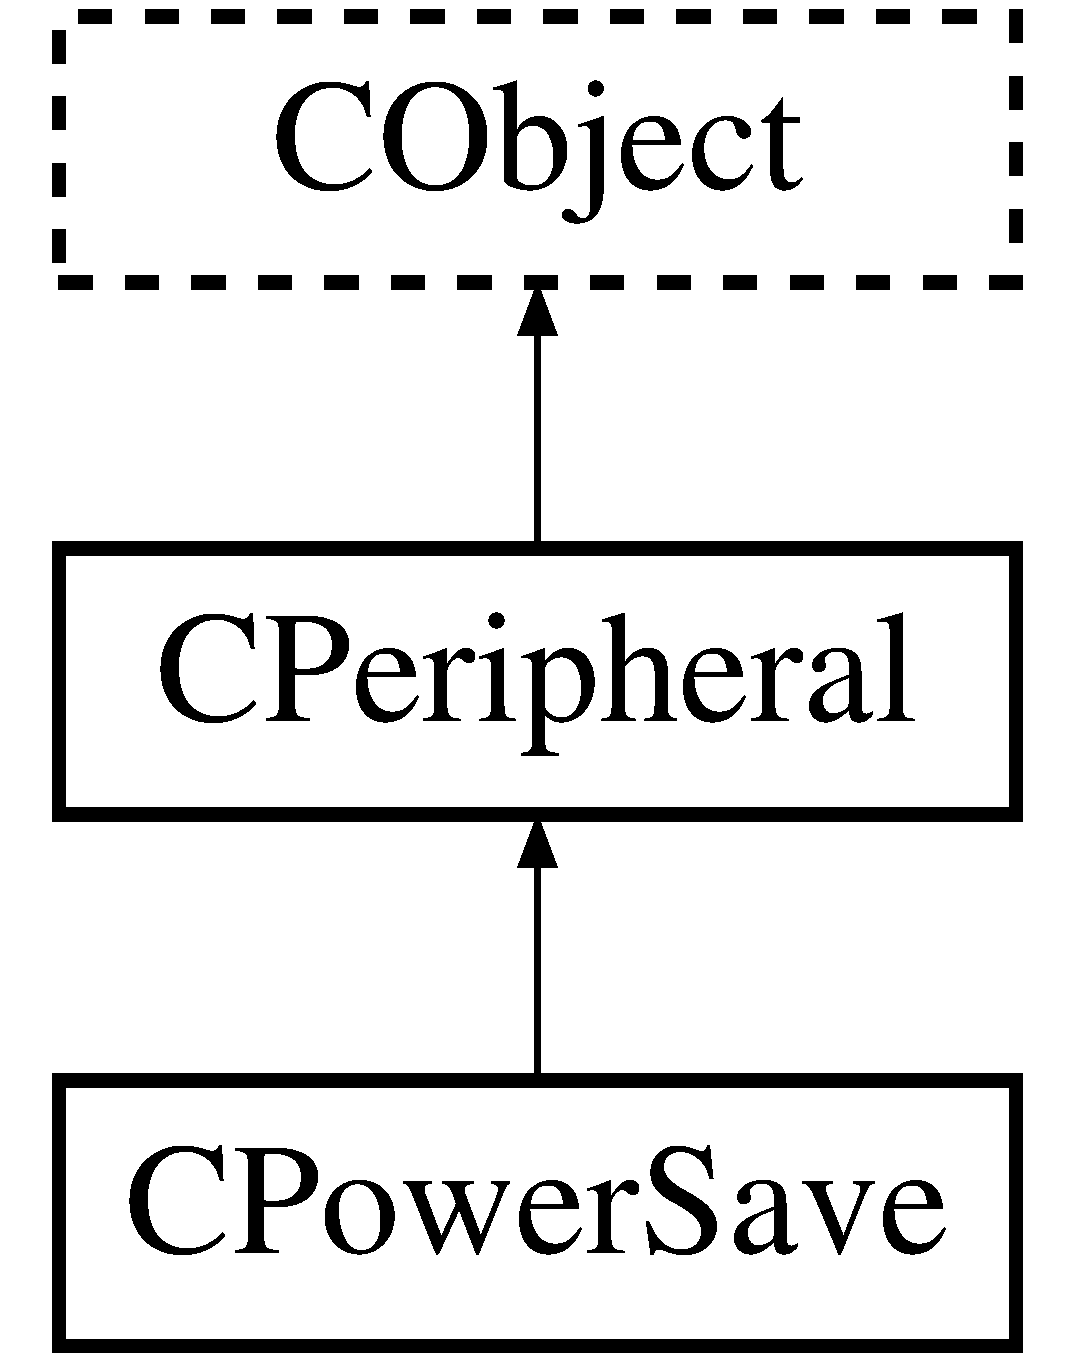
\includegraphics[height=3.000000cm]{class_c_power_save}
\end{center}
\end{figure}
\subsection*{Public Member Functions}
\begin{DoxyCompactItemize}
\item 
\hypertarget{class_c_power_save_a47741a6376b9b3065422d37d49851f25}{void {\bfseries enable} (P\-S\-\_\-\-M\-O\-D\-E\-\_\-\-T mode=D\-E\-E\-P\-\_\-\-S\-L\-E\-E\-P)}\label{class_c_power_save_a47741a6376b9b3065422d37d49851f25}

\item 
\hypertarget{class_c_power_save_a4311f52789a5e20f2a37ebddb1228e36}{void {\bfseries disable} ()}\label{class_c_power_save_a4311f52789a5e20f2a37ebddb1228e36}

\item 
\hypertarget{class_c_power_save_a646cda9a3b424a1cb4e1dbf5b9d4870f}{virtual void {\bfseries on\-Sleep} (uint32\-\_\-t ul\-Expected\-Idle\-Time)}\label{class_c_power_save_a646cda9a3b424a1cb4e1dbf5b9d4870f}

\item 
\hypertarget{class_c_power_save_a3c0304fe662448a763f8addb03a0f342}{virtual void {\bfseries on\-Wakeup} (uint32\-\_\-t $\ast$p\-Expected\-Idle\-Time)}\label{class_c_power_save_a3c0304fe662448a763f8addb03a0f342}

\item 
\hypertarget{class_c_power_save_ae7f5e81053c530c03deef192c10f93d5}{virtual bool {\bfseries is\-Enable} ()}\label{class_c_power_save_ae7f5e81053c530c03deef192c10f93d5}

\end{DoxyCompactItemize}
\subsection*{Protected Attributes}
\begin{DoxyCompactItemize}
\item 
\hypertarget{class_c_power_save_a3095ad5f6ba5d06364df1fd8304147ba}{uint32\-\_\-t {\bfseries m\-\_\-flag}}\label{class_c_power_save_a3095ad5f6ba5d06364df1fd8304147ba}

\item 
\hypertarget{class_c_power_save_afac4eec3245ca0555adb81ad15dad2a0}{\hyperlink{class_c_watchdog}{C\-Watchdog} {\bfseries m\-\_\-wdt}}\label{class_c_power_save_afac4eec3245ca0555adb81ad15dad2a0}

\end{DoxyCompactItemize}


The documentation for this class was generated from the following file\-:\begin{DoxyCompactItemize}
\item 
power.\-h\end{DoxyCompactItemize}

\hypertarget{class_c_pwm}{\section{C\-Pwm Class Reference}
\label{class_c_pwm}\index{C\-Pwm@{C\-Pwm}}
}


Pulse-\/width modulated output.  




{\ttfamily \#include \char`\"{}class/pwm.\-h\char`\"{}}

Inheritance diagram for C\-Pwm\-:\begin{figure}[H]
\begin{center}
\leavevmode
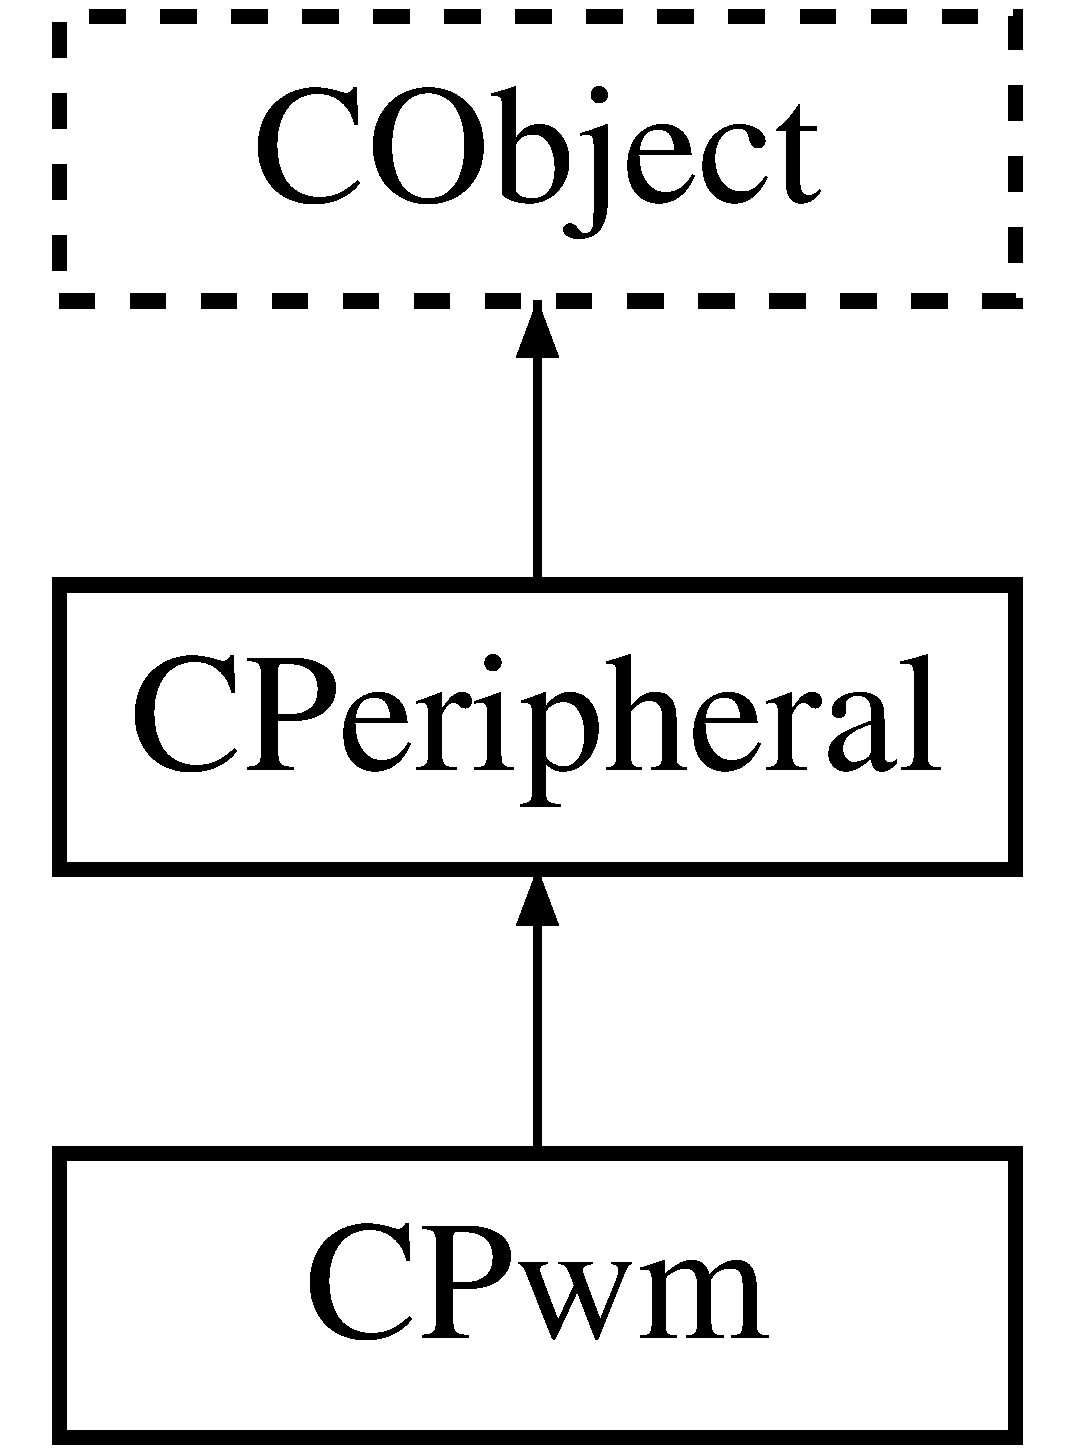
\includegraphics[height=3.000000cm]{d1/d9f/class_c_pwm}
\end{center}
\end{figure}
\subsection*{Public Member Functions}
\begin{DoxyCompactItemize}
\item 
\hyperlink{class_c_pwm_a53beaa27e8d3982351770f425dffb432}{C\-Pwm} (P\-W\-M\-\_\-\-C\-H\-\_\-\-T ch)
\item 
virtual void \hyperlink{class_c_pwm_a640f06df704cc299e45fafb9c1a1972e}{enable} ()
\item 
virtual void \hyperlink{class_c_pwm_a47c790491c994cc959bf204415be2aeb}{disable} ()
\item 
virtual void \hyperlink{class_c_pwm_ae0cb5e7e45453fb3fc049bada896c151}{duty\-Cycle} (float percentage)
\item 
virtual void \hyperlink{class_c_pwm_ae6ea4c5209e4f1360861371c7bf744e7}{pulse\-Width} (float sec)
\item 
virtual float \hyperlink{class_c_pwm_af69709834f0c179df1a6d8e7ad314930}{read} ()
\item 
void \hyperlink{class_c_pwm_a57cbfceb20e1f2970f45b5d1571431d1}{write} (float percentage)
\item 
void \hyperlink{class_c_pwm_aadc2ad3efd1afe9ae32919462c8286cb}{operator=} (float sec)
\item 
\hyperlink{class_c_pwm_a34dc590715ddb4b118132c69dad1140f}{operator float} ()
\item 
void \hyperlink{class_c_pwm_ae8fdd7f2337005c61ec995196de366de}{begin} ()
\item 
void \hyperlink{class_c_pwm_aea8cdf467fe4d3e1b3c1547dbfbce4ce}{end} ()
\end{DoxyCompactItemize}
\subsection*{Static Public Member Functions}
\begin{DoxyCompactItemize}
\item 
static void \hyperlink{class_c_pwm_aff0df75ef798c102015abedf86998366}{period} (float sec)
\item 
static void \hyperlink{class_c_pwm_a21081698744ec8596a9e922d3bedc8ed}{frequency} (uint32\-\_\-t f)
\end{DoxyCompactItemize}


\subsection{Detailed Description}
Pulse-\/width modulated output. 

\subsection{Constructor \& Destructor Documentation}
\hypertarget{class_c_pwm_a53beaa27e8d3982351770f425dffb432}{\index{C\-Pwm@{C\-Pwm}!C\-Pwm@{C\-Pwm}}
\index{C\-Pwm@{C\-Pwm}!CPwm@{C\-Pwm}}
\subsubsection[{C\-Pwm}]{\setlength{\rightskip}{0pt plus 5cm}C\-Pwm\-::\-C\-Pwm (
\begin{DoxyParamCaption}
\item[{P\-W\-M\-\_\-\-C\-H\-\_\-\-T}]{ch}
\end{DoxyParamCaption}
)}}\label{class_c_pwm_a53beaa27e8d3982351770f425dffb432}
Constructs a \hyperlink{class_c_pwm}{C\-Pwm} object to connect to the specified P\-W\-M channel. 
\begin{DoxyParams}{Parameters}
{\em ch} & ... are P\-W\-M\-\_\-\-C\-H\-\_\-\-T to specified a P\-W\-M channel to the object.\\
\hline
\end{DoxyParams}

\begin{DoxyCode}
Example:
        \hyperlink{class_c_pwm_aff0df75ef798c102015abedf86998366}{CPwm::period}(0.02); \textcolor{comment}{// Set PWM period time = 20ms}
        CPwm::start();      \textcolor{comment}{// Start the core PWM peripheral}

        \hyperlink{class_c_pwm}{CPwm} servo(PWM1);   \textcolor{comment}{// create a servo objecj}
        servo.dutyCycle(80);\textcolor{comment}{// set servo object to 80% dutyCycle}
        servo.begin();      \textcolor{comment}{// begin the servo PWM output}
\end{DoxyCode}


\begin{DoxyRemark}{Remarks}
to 'E\-N\-D' of the pin arguments is M\-U\-S\-T!! 
\end{DoxyRemark}


\subsection{Member Function Documentation}
\hypertarget{class_c_pwm_a640f06df704cc299e45fafb9c1a1972e}{\index{C\-Pwm@{C\-Pwm}!enable@{enable}}
\index{enable@{enable}!CPwm@{C\-Pwm}}
\subsubsection[{enable}]{\setlength{\rightskip}{0pt plus 5cm}virtual void C\-Pwm\-::enable (
\begin{DoxyParamCaption}
{}
\end{DoxyParamCaption}
)\hspace{0.3cm}{\ttfamily [virtual]}}}\label{class_c_pwm_a640f06df704cc299e45fafb9c1a1972e}
enable the P\-W\-M channel output \hypertarget{class_c_pwm_a47c790491c994cc959bf204415be2aeb}{\index{C\-Pwm@{C\-Pwm}!disable@{disable}}
\index{disable@{disable}!CPwm@{C\-Pwm}}
\subsubsection[{disable}]{\setlength{\rightskip}{0pt plus 5cm}virtual void C\-Pwm\-::disable (
\begin{DoxyParamCaption}
{}
\end{DoxyParamCaption}
)\hspace{0.3cm}{\ttfamily [virtual]}}}\label{class_c_pwm_a47c790491c994cc959bf204415be2aeb}
disable of the P\-W\-M channel output \hypertarget{class_c_pwm_ae0cb5e7e45453fb3fc049bada896c151}{\index{C\-Pwm@{C\-Pwm}!duty\-Cycle@{duty\-Cycle}}
\index{duty\-Cycle@{duty\-Cycle}!CPwm@{C\-Pwm}}
\subsubsection[{duty\-Cycle}]{\setlength{\rightskip}{0pt plus 5cm}virtual void C\-Pwm\-::duty\-Cycle (
\begin{DoxyParamCaption}
\item[{float}]{percentage}
\end{DoxyParamCaption}
)\hspace{0.3cm}{\ttfamily [virtual]}}}\label{class_c_pwm_ae0cb5e7e45453fb3fc049bada896c151}
Set the output duty-\/cycle, specified as a percentage (float) \hypertarget{class_c_pwm_ae6ea4c5209e4f1360861371c7bf744e7}{\index{C\-Pwm@{C\-Pwm}!pulse\-Width@{pulse\-Width}}
\index{pulse\-Width@{pulse\-Width}!CPwm@{C\-Pwm}}
\subsubsection[{pulse\-Width}]{\setlength{\rightskip}{0pt plus 5cm}virtual void C\-Pwm\-::pulse\-Width (
\begin{DoxyParamCaption}
\item[{float}]{sec}
\end{DoxyParamCaption}
)\hspace{0.3cm}{\ttfamily [virtual]}}}\label{class_c_pwm_ae6ea4c5209e4f1360861371c7bf744e7}
Set the P\-W\-M pulse-\/width, specified in seconds (float) \hypertarget{class_c_pwm_af69709834f0c179df1a6d8e7ad314930}{\index{C\-Pwm@{C\-Pwm}!read@{read}}
\index{read@{read}!CPwm@{C\-Pwm}}
\subsubsection[{read}]{\setlength{\rightskip}{0pt plus 5cm}virtual float C\-Pwm\-::read (
\begin{DoxyParamCaption}
{}
\end{DoxyParamCaption}
)\hspace{0.3cm}{\ttfamily [virtual]}}}\label{class_c_pwm_af69709834f0c179df1a6d8e7ad314930}
\hypertarget{class_c_pwm_a57cbfceb20e1f2970f45b5d1571431d1}{\index{C\-Pwm@{C\-Pwm}!write@{write}}
\index{write@{write}!CPwm@{C\-Pwm}}
\subsubsection[{write}]{\setlength{\rightskip}{0pt plus 5cm}void C\-Pwm\-::write (
\begin{DoxyParamCaption}
\item[{float}]{percentage}
\end{DoxyParamCaption}
)\hspace{0.3cm}{\ttfamily [inline]}}}\label{class_c_pwm_a57cbfceb20e1f2970f45b5d1571431d1}
Set output duty-\/cycle; inline function call to the member \hyperlink{class_c_pwm_ae0cb5e7e45453fb3fc049bada896c151}{duty\-Cycle()} \hypertarget{class_c_pwm_aadc2ad3efd1afe9ae32919462c8286cb}{\index{C\-Pwm@{C\-Pwm}!operator=@{operator=}}
\index{operator=@{operator=}!CPwm@{C\-Pwm}}
\subsubsection[{operator=}]{\setlength{\rightskip}{0pt plus 5cm}void C\-Pwm\-::operator= (
\begin{DoxyParamCaption}
\item[{float}]{sec}
\end{DoxyParamCaption}
)\hspace{0.3cm}{\ttfamily [inline]}}}\label{class_c_pwm_aadc2ad3efd1afe9ae32919462c8286cb}
A shorthand to call the member \hyperlink{class_c_pwm_ae6ea4c5209e4f1360861371c7bf744e7}{pulse\-Width()} \hypertarget{class_c_pwm_a34dc590715ddb4b118132c69dad1140f}{\index{C\-Pwm@{C\-Pwm}!operator float@{operator float}}
\index{operator float@{operator float}!CPwm@{C\-Pwm}}
\subsubsection[{operator float}]{\setlength{\rightskip}{0pt plus 5cm}C\-Pwm\-::operator float (
\begin{DoxyParamCaption}
{}
\end{DoxyParamCaption}
)\hspace{0.3cm}{\ttfamily [inline]}}}\label{class_c_pwm_a34dc590715ddb4b118132c69dad1140f}
\hypertarget{class_c_pwm_aff0df75ef798c102015abedf86998366}{\index{C\-Pwm@{C\-Pwm}!period@{period}}
\index{period@{period}!CPwm@{C\-Pwm}}
\subsubsection[{period}]{\setlength{\rightskip}{0pt plus 5cm}static void C\-Pwm\-::period (
\begin{DoxyParamCaption}
\item[{float}]{sec}
\end{DoxyParamCaption}
)\hspace{0.3cm}{\ttfamily [static]}}}\label{class_c_pwm_aff0df75ef798c102015abedf86998366}
A static member function. Set the P\-W\-M M\-A\-I\-N period (or frequency), specified in seconds (float). \hypertarget{class_c_pwm_a21081698744ec8596a9e922d3bedc8ed}{\index{C\-Pwm@{C\-Pwm}!frequency@{frequency}}
\index{frequency@{frequency}!CPwm@{C\-Pwm}}
\subsubsection[{frequency}]{\setlength{\rightskip}{0pt plus 5cm}static void C\-Pwm\-::frequency (
\begin{DoxyParamCaption}
\item[{uint32\-\_\-t}]{f}
\end{DoxyParamCaption}
)\hspace{0.3cm}{\ttfamily [static]}}}\label{class_c_pwm_a21081698744ec8596a9e922d3bedc8ed}
\hypertarget{class_c_pwm_ae8fdd7f2337005c61ec995196de366de}{\index{C\-Pwm@{C\-Pwm}!begin@{begin}}
\index{begin@{begin}!CPwm@{C\-Pwm}}
\subsubsection[{begin}]{\setlength{\rightskip}{0pt plus 5cm}void C\-Pwm\-::begin (
\begin{DoxyParamCaption}
{}
\end{DoxyParamCaption}
)\hspace{0.3cm}{\ttfamily [inline]}}}\label{class_c_pwm_ae8fdd7f2337005c61ec995196de366de}
inline functions \hypertarget{class_c_pwm_aea8cdf467fe4d3e1b3c1547dbfbce4ce}{\index{C\-Pwm@{C\-Pwm}!end@{end}}
\index{end@{end}!CPwm@{C\-Pwm}}
\subsubsection[{end}]{\setlength{\rightskip}{0pt plus 5cm}void C\-Pwm\-::end (
\begin{DoxyParamCaption}
{}
\end{DoxyParamCaption}
)\hspace{0.3cm}{\ttfamily [inline]}}}\label{class_c_pwm_aea8cdf467fe4d3e1b3c1547dbfbce4ce}


The documentation for this class was generated from the following file\-:\begin{DoxyCompactItemize}
\item 
pwm.\-h\end{DoxyCompactItemize}

\hypertarget{class_c_r_c16}{\section{C\-R\-C16 Class Reference}
\label{class_c_r_c16}\index{C\-R\-C16@{C\-R\-C16}}
}


{\ttfamily \#include $<$crc16.\-h$>$}

Inheritance diagram for C\-R\-C16\-:\begin{figure}[H]
\begin{center}
\leavevmode
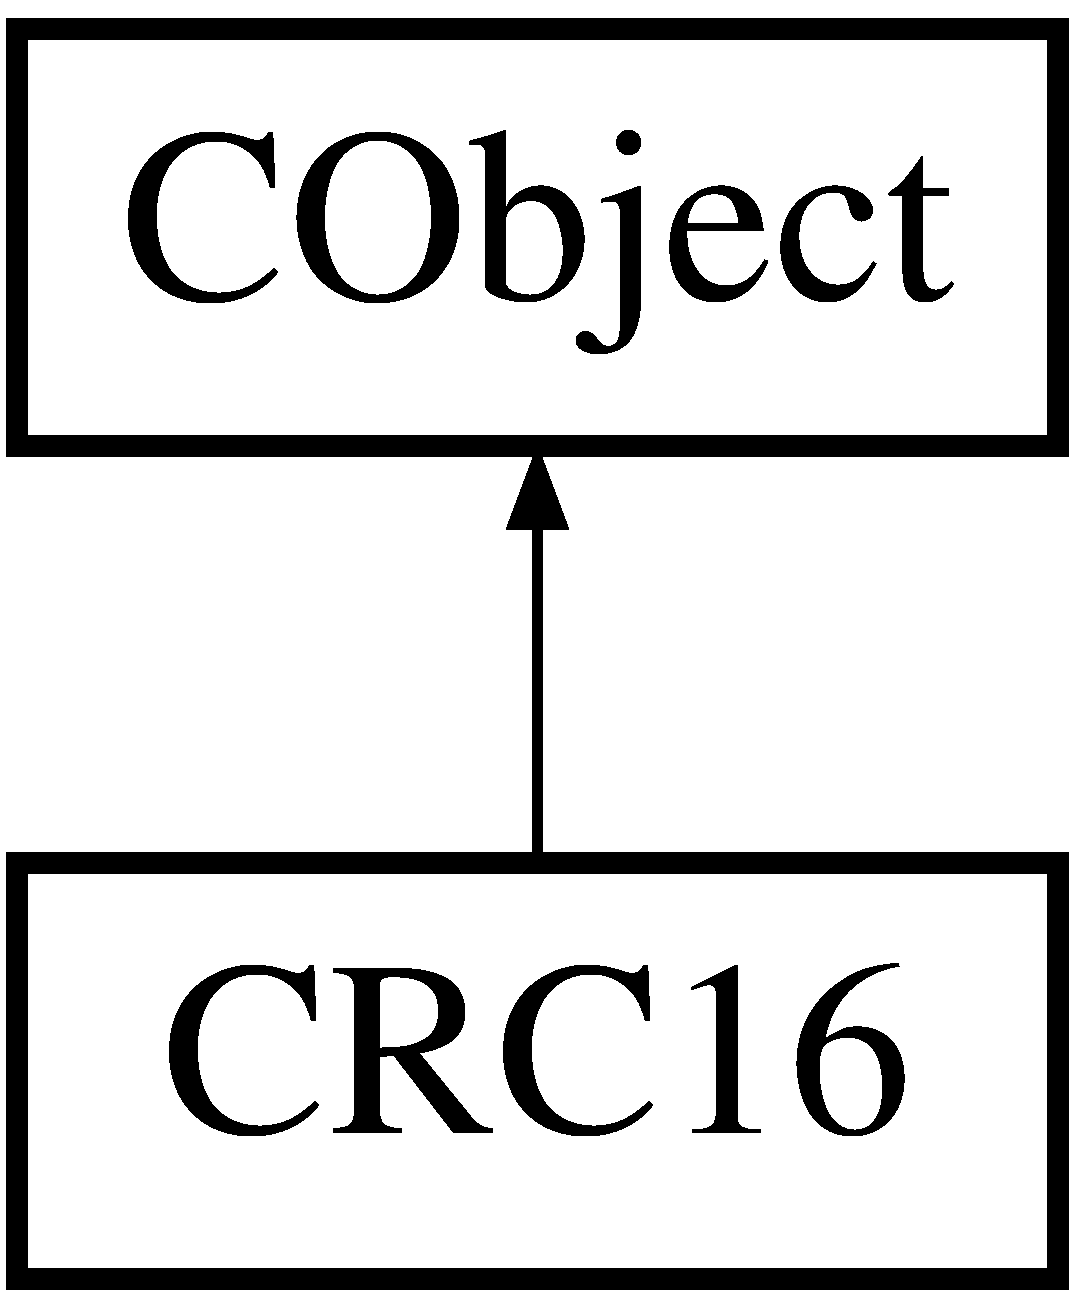
\includegraphics[height=2.000000cm]{d5/df3/class_c_r_c16}
\end{center}
\end{figure}
\subsection*{Public Member Functions}
\begin{DoxyCompactItemize}
\item 
\hyperlink{class_c_r_c16_a2317eff72b4509289399f5c6b6306db2}{C\-R\-C16} (uint16\-\_\-t init=0xffff, uint16\-\_\-t poly=0x1021)
\item 
virtual \hyperlink{class_c_r_c16_a017c6bb359a7403dedc5db838ceb627d}{$\sim$\-C\-R\-C16} ()
\item 
virtual void \hyperlink{class_c_r_c16_ad948d7638a1d07540db96cb649ce0d52}{reset} ()
\item 
virtual void \hyperlink{class_c_r_c16_afd577ee51489a3e07c4de201b8a3fdf4}{update} (uint8\-\_\-t data)
\item 
virtual void \hyperlink{class_c_r_c16_aea5d7fae41950ebc9ab79ec0445900f5}{update} (uint8\-\_\-t $\ast$buf, int length)
\item 
virtual uint16\-\_\-t \hyperlink{class_c_r_c16_aa70e96e936eea96361292dfc3f1a71fc}{result} ()
\item 
\hyperlink{class_c_r_c16_ac6704db61d9df8cf08e8f5697b7f8b31}{operator uint16\-\_\-t} ()
\end{DoxyCompactItemize}
\subsection*{Protected Attributes}
\begin{DoxyCompactItemize}
\item 
uint16\-\_\-t \hyperlink{class_c_r_c16_ae3d38db69627b3335b5a5f008057f98c}{m\-\_\-poly}
\item 
uint16\-\_\-t \hyperlink{class_c_r_c16_a85c28fd3fef555b4d25b0d18186fae6a}{m\-\_\-init}
\item 
uint16\-\_\-t \hyperlink{class_c_r_c16_a010ae9e2779e15bd4baf9a56980cd272}{m\-\_\-crc}
\end{DoxyCompactItemize}


\subsection{Constructor \& Destructor Documentation}
\hypertarget{class_c_r_c16_a2317eff72b4509289399f5c6b6306db2}{\index{C\-R\-C16@{C\-R\-C16}!C\-R\-C16@{C\-R\-C16}}
\index{C\-R\-C16@{C\-R\-C16}!CRC16@{C\-R\-C16}}
\subsubsection[{C\-R\-C16}]{\setlength{\rightskip}{0pt plus 5cm}C\-R\-C16\-::\-C\-R\-C16 (
\begin{DoxyParamCaption}
\item[{uint16\-\_\-t}]{init = {\ttfamily 0xffff}, }
\item[{uint16\-\_\-t}]{poly = {\ttfamily 0x1021}}
\end{DoxyParamCaption}
)}}\label{class_c_r_c16_a2317eff72b4509289399f5c6b6306db2}
\hypertarget{class_c_r_c16_a017c6bb359a7403dedc5db838ceb627d}{\index{C\-R\-C16@{C\-R\-C16}!$\sim$\-C\-R\-C16@{$\sim$\-C\-R\-C16}}
\index{$\sim$\-C\-R\-C16@{$\sim$\-C\-R\-C16}!CRC16@{C\-R\-C16}}
\subsubsection[{$\sim$\-C\-R\-C16}]{\setlength{\rightskip}{0pt plus 5cm}virtual C\-R\-C16\-::$\sim$\-C\-R\-C16 (
\begin{DoxyParamCaption}
{}
\end{DoxyParamCaption}
)\hspace{0.3cm}{\ttfamily [virtual]}}}\label{class_c_r_c16_a017c6bb359a7403dedc5db838ceb627d}


\subsection{Member Function Documentation}
\hypertarget{class_c_r_c16_ad948d7638a1d07540db96cb649ce0d52}{\index{C\-R\-C16@{C\-R\-C16}!reset@{reset}}
\index{reset@{reset}!CRC16@{C\-R\-C16}}
\subsubsection[{reset}]{\setlength{\rightskip}{0pt plus 5cm}virtual void C\-R\-C16\-::reset (
\begin{DoxyParamCaption}
{}
\end{DoxyParamCaption}
)\hspace{0.3cm}{\ttfamily [virtual]}}}\label{class_c_r_c16_ad948d7638a1d07540db96cb649ce0d52}
\hypertarget{class_c_r_c16_afd577ee51489a3e07c4de201b8a3fdf4}{\index{C\-R\-C16@{C\-R\-C16}!update@{update}}
\index{update@{update}!CRC16@{C\-R\-C16}}
\subsubsection[{update}]{\setlength{\rightskip}{0pt plus 5cm}virtual void C\-R\-C16\-::update (
\begin{DoxyParamCaption}
\item[{uint8\-\_\-t}]{data}
\end{DoxyParamCaption}
)\hspace{0.3cm}{\ttfamily [virtual]}}}\label{class_c_r_c16_afd577ee51489a3e07c4de201b8a3fdf4}
\hypertarget{class_c_r_c16_aea5d7fae41950ebc9ab79ec0445900f5}{\index{C\-R\-C16@{C\-R\-C16}!update@{update}}
\index{update@{update}!CRC16@{C\-R\-C16}}
\subsubsection[{update}]{\setlength{\rightskip}{0pt plus 5cm}virtual void C\-R\-C16\-::update (
\begin{DoxyParamCaption}
\item[{uint8\-\_\-t $\ast$}]{buf, }
\item[{int}]{length}
\end{DoxyParamCaption}
)\hspace{0.3cm}{\ttfamily [virtual]}}}\label{class_c_r_c16_aea5d7fae41950ebc9ab79ec0445900f5}
\hypertarget{class_c_r_c16_aa70e96e936eea96361292dfc3f1a71fc}{\index{C\-R\-C16@{C\-R\-C16}!result@{result}}
\index{result@{result}!CRC16@{C\-R\-C16}}
\subsubsection[{result}]{\setlength{\rightskip}{0pt plus 5cm}virtual uint16\-\_\-t C\-R\-C16\-::result (
\begin{DoxyParamCaption}
{}
\end{DoxyParamCaption}
)\hspace{0.3cm}{\ttfamily [virtual]}}}\label{class_c_r_c16_aa70e96e936eea96361292dfc3f1a71fc}
\hypertarget{class_c_r_c16_ac6704db61d9df8cf08e8f5697b7f8b31}{\index{C\-R\-C16@{C\-R\-C16}!operator uint16\-\_\-t@{operator uint16\-\_\-t}}
\index{operator uint16\-\_\-t@{operator uint16\-\_\-t}!CRC16@{C\-R\-C16}}
\subsubsection[{operator uint16\-\_\-t}]{\setlength{\rightskip}{0pt plus 5cm}C\-R\-C16\-::operator uint16\-\_\-t (
\begin{DoxyParamCaption}
{}
\end{DoxyParamCaption}
)\hspace{0.3cm}{\ttfamily [inline]}}}\label{class_c_r_c16_ac6704db61d9df8cf08e8f5697b7f8b31}


\subsection{Member Data Documentation}
\hypertarget{class_c_r_c16_ae3d38db69627b3335b5a5f008057f98c}{\index{C\-R\-C16@{C\-R\-C16}!m\-\_\-poly@{m\-\_\-poly}}
\index{m\-\_\-poly@{m\-\_\-poly}!CRC16@{C\-R\-C16}}
\subsubsection[{m\-\_\-poly}]{\setlength{\rightskip}{0pt plus 5cm}uint16\-\_\-t C\-R\-C16\-::m\-\_\-poly\hspace{0.3cm}{\ttfamily [protected]}}}\label{class_c_r_c16_ae3d38db69627b3335b5a5f008057f98c}
\hypertarget{class_c_r_c16_a85c28fd3fef555b4d25b0d18186fae6a}{\index{C\-R\-C16@{C\-R\-C16}!m\-\_\-init@{m\-\_\-init}}
\index{m\-\_\-init@{m\-\_\-init}!CRC16@{C\-R\-C16}}
\subsubsection[{m\-\_\-init}]{\setlength{\rightskip}{0pt plus 5cm}uint16\-\_\-t C\-R\-C16\-::m\-\_\-init\hspace{0.3cm}{\ttfamily [protected]}}}\label{class_c_r_c16_a85c28fd3fef555b4d25b0d18186fae6a}
\hypertarget{class_c_r_c16_a010ae9e2779e15bd4baf9a56980cd272}{\index{C\-R\-C16@{C\-R\-C16}!m\-\_\-crc@{m\-\_\-crc}}
\index{m\-\_\-crc@{m\-\_\-crc}!CRC16@{C\-R\-C16}}
\subsubsection[{m\-\_\-crc}]{\setlength{\rightskip}{0pt plus 5cm}uint16\-\_\-t C\-R\-C16\-::m\-\_\-crc\hspace{0.3cm}{\ttfamily [protected]}}}\label{class_c_r_c16_a010ae9e2779e15bd4baf9a56980cd272}


The documentation for this class was generated from the following file\-:\begin{DoxyCompactItemize}
\item 
crc16.\-h\end{DoxyCompactItemize}

\hypertarget{class_c_semaphore}{\section{C\-Semaphore Class Reference}
\label{class_c_semaphore}\index{C\-Semaphore@{C\-Semaphore}}
}


{\ttfamily \#include \char`\"{}class/semaphore.\-h\char`\"{}}

Inheritance diagram for C\-Semaphore\-:\begin{figure}[H]
\begin{center}
\leavevmode
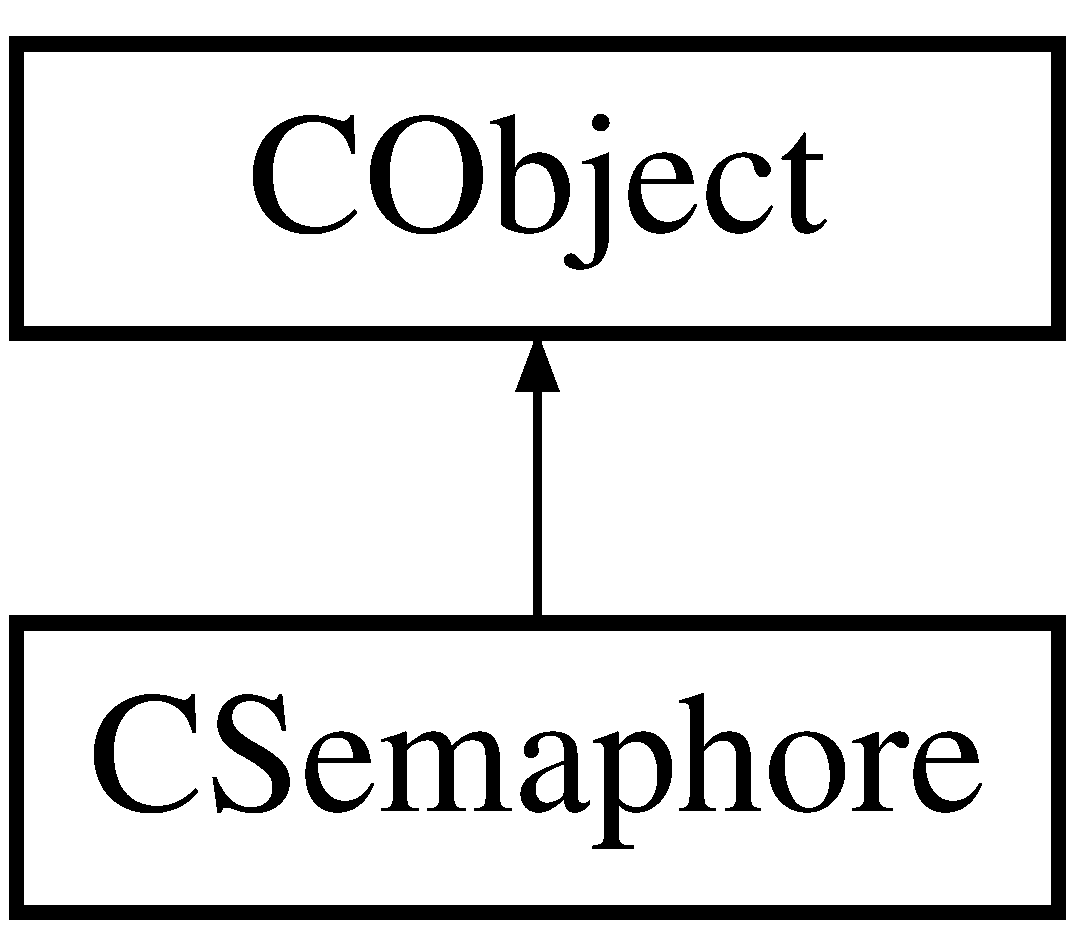
\includegraphics[height=2.000000cm]{d0/d06/class_c_semaphore}
\end{center}
\end{figure}
\subsection*{Public Member Functions}
\begin{DoxyCompactItemize}
\item 
virtual bool \hyperlink{class_c_semaphore_af4e913cd2861355f8be2211ae21753ba}{counting} (int count, int init=0)
\item 
virtual bool \hyperlink{class_c_semaphore_a0fc078dfd286cb3321c6cbaf7bcbb7b2}{binary} ()
\item 
virtual bool \hyperlink{class_c_semaphore_abad6f22e40a0d911e38ade968f4d801a}{wait} (int timeout=M\-A\-X\-\_\-\-D\-E\-L\-A\-Y\-\_\-\-T\-I\-M\-E)
\item 
virtual int \hyperlink{class_c_semaphore_aa1a25ff1be26f8dfdd0f008aeabec8b1}{release} (bool from\-I\-S\-R=false)
\item 
virtual int \hyperlink{class_c_semaphore_a2302ceb8f2f9e1bef3381f457589177d}{waiting} ()
\end{DoxyCompactItemize}


\subsection{Detailed Description}
The \hyperlink{class_c_semaphore}{C\-Semaphore} class provides two kinds semaphore which counting and binary. \begin{DoxyNote}{Note}
\hyperlink{class_c_semaphore}{C\-Semaphore} cannot be used before a call to member counting or binary. 
\end{DoxyNote}


\subsection{Member Function Documentation}
\hypertarget{class_c_semaphore_af4e913cd2861355f8be2211ae21753ba}{\index{C\-Semaphore@{C\-Semaphore}!counting@{counting}}
\index{counting@{counting}!CSemaphore@{C\-Semaphore}}
\subsubsection[{counting}]{\setlength{\rightskip}{0pt plus 5cm}virtual bool C\-Semaphore\-::counting (
\begin{DoxyParamCaption}
\item[{int}]{count, }
\item[{int}]{init = {\ttfamily 0}}
\end{DoxyParamCaption}
)\hspace{0.3cm}{\ttfamily [virtual]}}}\label{class_c_semaphore_af4e913cd2861355f8be2211ae21753ba}
Call the member function to creates a counting semaphore. 
\begin{DoxyParams}{Parameters}
{\em count} & is a integer value to specified the maximum count thate can be reached. \\
\hline
{\em init} & is a integer value to assigned to the semaphore when it is created. \\
\hline
\end{DoxyParams}
\begin{DoxyReturn}{Returns}
true if create semaphore successful; otherwise, failed. 
\end{DoxyReturn}
\hypertarget{class_c_semaphore_a0fc078dfd286cb3321c6cbaf7bcbb7b2}{\index{C\-Semaphore@{C\-Semaphore}!binary@{binary}}
\index{binary@{binary}!CSemaphore@{C\-Semaphore}}
\subsubsection[{binary}]{\setlength{\rightskip}{0pt plus 5cm}virtual bool C\-Semaphore\-::binary (
\begin{DoxyParamCaption}
{}
\end{DoxyParamCaption}
)\hspace{0.3cm}{\ttfamily [virtual]}}}\label{class_c_semaphore_a0fc078dfd286cb3321c6cbaf7bcbb7b2}
Call the member function to creates a binary semaphore. \begin{DoxyReturn}{Returns}
true if create semaphore successful; otherwise, failed. 
\end{DoxyReturn}
\begin{DoxyNote}{Note}
Binary semaphores and mutexes are very similar but have some subtle differences\-: Mutexes include a priority inheritance mechanism, binary semaphores do not. This makes binary semaphores the better choice for implementing synchronisation (between tasks or between tasks and an interrupt), and mutexes the better choice for implementing simple mutual exclusion. 
\end{DoxyNote}
\hypertarget{class_c_semaphore_abad6f22e40a0d911e38ade968f4d801a}{\index{C\-Semaphore@{C\-Semaphore}!wait@{wait}}
\index{wait@{wait}!CSemaphore@{C\-Semaphore}}
\subsubsection[{wait}]{\setlength{\rightskip}{0pt plus 5cm}virtual bool C\-Semaphore\-::wait (
\begin{DoxyParamCaption}
\item[{int}]{timeout = {\ttfamily MAX\-\_\-DELAY\-\_\-TIME}}
\end{DoxyParamCaption}
)\hspace{0.3cm}{\ttfamily [virtual]}}}\label{class_c_semaphore_abad6f22e40a0d911e38ade968f4d801a}
Call the member function to wait a semaphore available. 
\begin{DoxyParams}{Parameters}
{\em timeout} & is a integer value to specified the millisecond to wait for the semaphore to become available. \\
\hline
\end{DoxyParams}
\begin{DoxyReturn}{Returns}
true if create semaphore successful; otherwise, failed.
\end{DoxyReturn}

\begin{DoxyCode}
Example:
        \hyperlink{class_c_semaphore}{CSemaphore} semLED;

        \textcolor{comment}{// resource}
        \hyperlink{class_c_bus}{CBus} leds(\hyperlink{group___enumerations_gga65a2241721e4acb573e0c3fe29ac432fadac6477842247cab1a8c02c65f431b44}{LED1}, \hyperlink{group___enumerations_gga65a2241721e4acb573e0c3fe29ac432fa8379bbaa96d151e6adac488b2a147b7a}{LED2}, \hyperlink{group___enumerations_gga65a2241721e4acb573e0c3fe29ac432fa5dec293e081e0fc78369c842fab8452b}{LED3}, \hyperlink{group___enumerations_gga65a2241721e4acb573e0c3fe29ac432fad60e39b8d1701d30aa64f80343217342}{LED4}, \hyperlink{group___enumerations_gga65a2241721e4acb573e0c3fe29ac432fadc6f24fd6915a3f2786a1b7045406924}{END});
        \textcolor{keywordtype}{int}  index;

        \textcolor{comment}{// task1}
        \textcolor{keyword}{class }Task1: \textcolor{keyword}{public} \hyperlink{class_c_thread}{CThread} \{
        \textcolor{keyword}{protected}:
            \textcolor{keyword}{virtual} \textcolor{keywordtype}{void} run() \{
                \textcolor{keywordflow}{while}(1) \{
                    index = rand() % 4;     \textcolor{comment}{// get a random value in 0~3.}
                    semLED.\hyperlink{class_c_semaphore_aa1a25ff1be26f8dfdd0f008aeabec8b1}{release}();       \textcolor{comment}{// release resource.}
                    sleep(500);
                \}
            \}
        \};

        \textcolor{comment}{// task2}
        \textcolor{keyword}{class }Task2: \textcolor{keyword}{public} \hyperlink{class_c_thread}{CThread} \{
    \textcolor{keyword}{protected}:
            \textcolor{keyword}{virtual} \textcolor{keywordtype}{void} run() \{
                \textcolor{keywordflow}{while}(1) \{
                    semLED.\hyperlink{class_c_semaphore_abad6f22e40a0d911e38ade968f4d801a}{wait}();          \textcolor{comment}{// wait resource available.}
                    leds[index] = !leds[index];
                \}
            \}
        \}

        \textcolor{keywordtype}{void} main() \{
            ...
            semLED.\hyperlink{class_c_semaphore_a0fc078dfd286cb3321c6cbaf7bcbb7b2}{binary}();    \textcolor{comment}{// set the semaphore in binary mode}
            ...
        \}
\end{DoxyCode}
 \hypertarget{class_c_semaphore_aa1a25ff1be26f8dfdd0f008aeabec8b1}{\index{C\-Semaphore@{C\-Semaphore}!release@{release}}
\index{release@{release}!CSemaphore@{C\-Semaphore}}
\subsubsection[{release}]{\setlength{\rightskip}{0pt plus 5cm}virtual int C\-Semaphore\-::release (
\begin{DoxyParamCaption}
\item[{bool}]{from\-I\-S\-R = {\ttfamily false}}
\end{DoxyParamCaption}
)\hspace{0.3cm}{\ttfamily [virtual]}}}\label{class_c_semaphore_aa1a25ff1be26f8dfdd0f008aeabec8b1}
Call the member function to release a semaphore. 
\begin{DoxyParams}{Parameters}
{\em from\-I\-S\-R} & is a boolean to specified the release occur from interrupt routine. (internal used) \\
\hline
\end{DoxyParams}
\begin{DoxyReturn}{Returns}
a integer value to identify the context switch wake. (internal used)
\end{DoxyReturn}

\begin{DoxyCode}
Example:
        \hyperlink{class_c_semaphore}{CSemaphore} semLED;

        \textcolor{comment}{// resource}
        \hyperlink{class_c_bus}{CBus} leds(\hyperlink{group___enumerations_gga65a2241721e4acb573e0c3fe29ac432fadac6477842247cab1a8c02c65f431b44}{LED1}, \hyperlink{group___enumerations_gga65a2241721e4acb573e0c3fe29ac432fa8379bbaa96d151e6adac488b2a147b7a}{LED2}, \hyperlink{group___enumerations_gga65a2241721e4acb573e0c3fe29ac432fa5dec293e081e0fc78369c842fab8452b}{LED3}, \hyperlink{group___enumerations_gga65a2241721e4acb573e0c3fe29ac432fad60e39b8d1701d30aa64f80343217342}{LED4}, \hyperlink{group___enumerations_gga65a2241721e4acb573e0c3fe29ac432fadc6f24fd6915a3f2786a1b7045406924}{END});
        \textcolor{keywordtype}{int}  index;

        \textcolor{comment}{// task1}
        \textcolor{keyword}{class }Task1: \textcolor{keyword}{public} \hyperlink{class_c_thread}{CThread} \{
        \textcolor{keyword}{protected}:
            \textcolor{keyword}{virtual} \textcolor{keywordtype}{void} run() \{
                \textcolor{keywordflow}{while}(1) \{
                    index = rand() % 4;     \textcolor{comment}{// get a random value in 0~3.}
                    semLED.\hyperlink{class_c_semaphore_aa1a25ff1be26f8dfdd0f008aeabec8b1}{release}();       \textcolor{comment}{// release resource.}
                    sleep(500);
                \}
            \}
        \};

        \textcolor{comment}{// task2}
        \textcolor{keyword}{class }Task2: \textcolor{keyword}{public} \hyperlink{class_c_thread}{CThread} \{
    \textcolor{keyword}{protected}:
            \textcolor{keyword}{virtual} \textcolor{keywordtype}{void} run() \{
                \textcolor{keywordflow}{while}(1) \{
                    semLED.\hyperlink{class_c_semaphore_abad6f22e40a0d911e38ade968f4d801a}{wait}();          \textcolor{comment}{// wait resource available.}
                    leds[index] = !leds[index];
                \}
            \}
        \}

        \textcolor{keywordtype}{void} main() \{
            ...
            semLED.\hyperlink{class_c_semaphore_a0fc078dfd286cb3321c6cbaf7bcbb7b2}{binary}();    \textcolor{comment}{// set the semaphore in binary mode}
            ...
        \}
\end{DoxyCode}
 \hypertarget{class_c_semaphore_a2302ceb8f2f9e1bef3381f457589177d}{\index{C\-Semaphore@{C\-Semaphore}!waiting@{waiting}}
\index{waiting@{waiting}!CSemaphore@{C\-Semaphore}}
\subsubsection[{waiting}]{\setlength{\rightskip}{0pt plus 5cm}virtual int C\-Semaphore\-::waiting (
\begin{DoxyParamCaption}
{}
\end{DoxyParamCaption}
)\hspace{0.3cm}{\ttfamily [virtual]}}}\label{class_c_semaphore_a2302ceb8f2f9e1bef3381f457589177d}
Number of task in waiting 

The documentation for this class was generated from the following file\-:\begin{DoxyCompactItemize}
\item 
semaphore.\-h\end{DoxyCompactItemize}

\hypertarget{class_c_serial}{\section{C\-Serial Class Reference}
\label{class_c_serial}\index{C\-Serial@{C\-Serial}}
}


{\ttfamily \#include \char`\"{}class/serial.\-h\char`\"{}}

Inheritance diagram for C\-Serial\-:\begin{figure}[H]
\begin{center}
\leavevmode
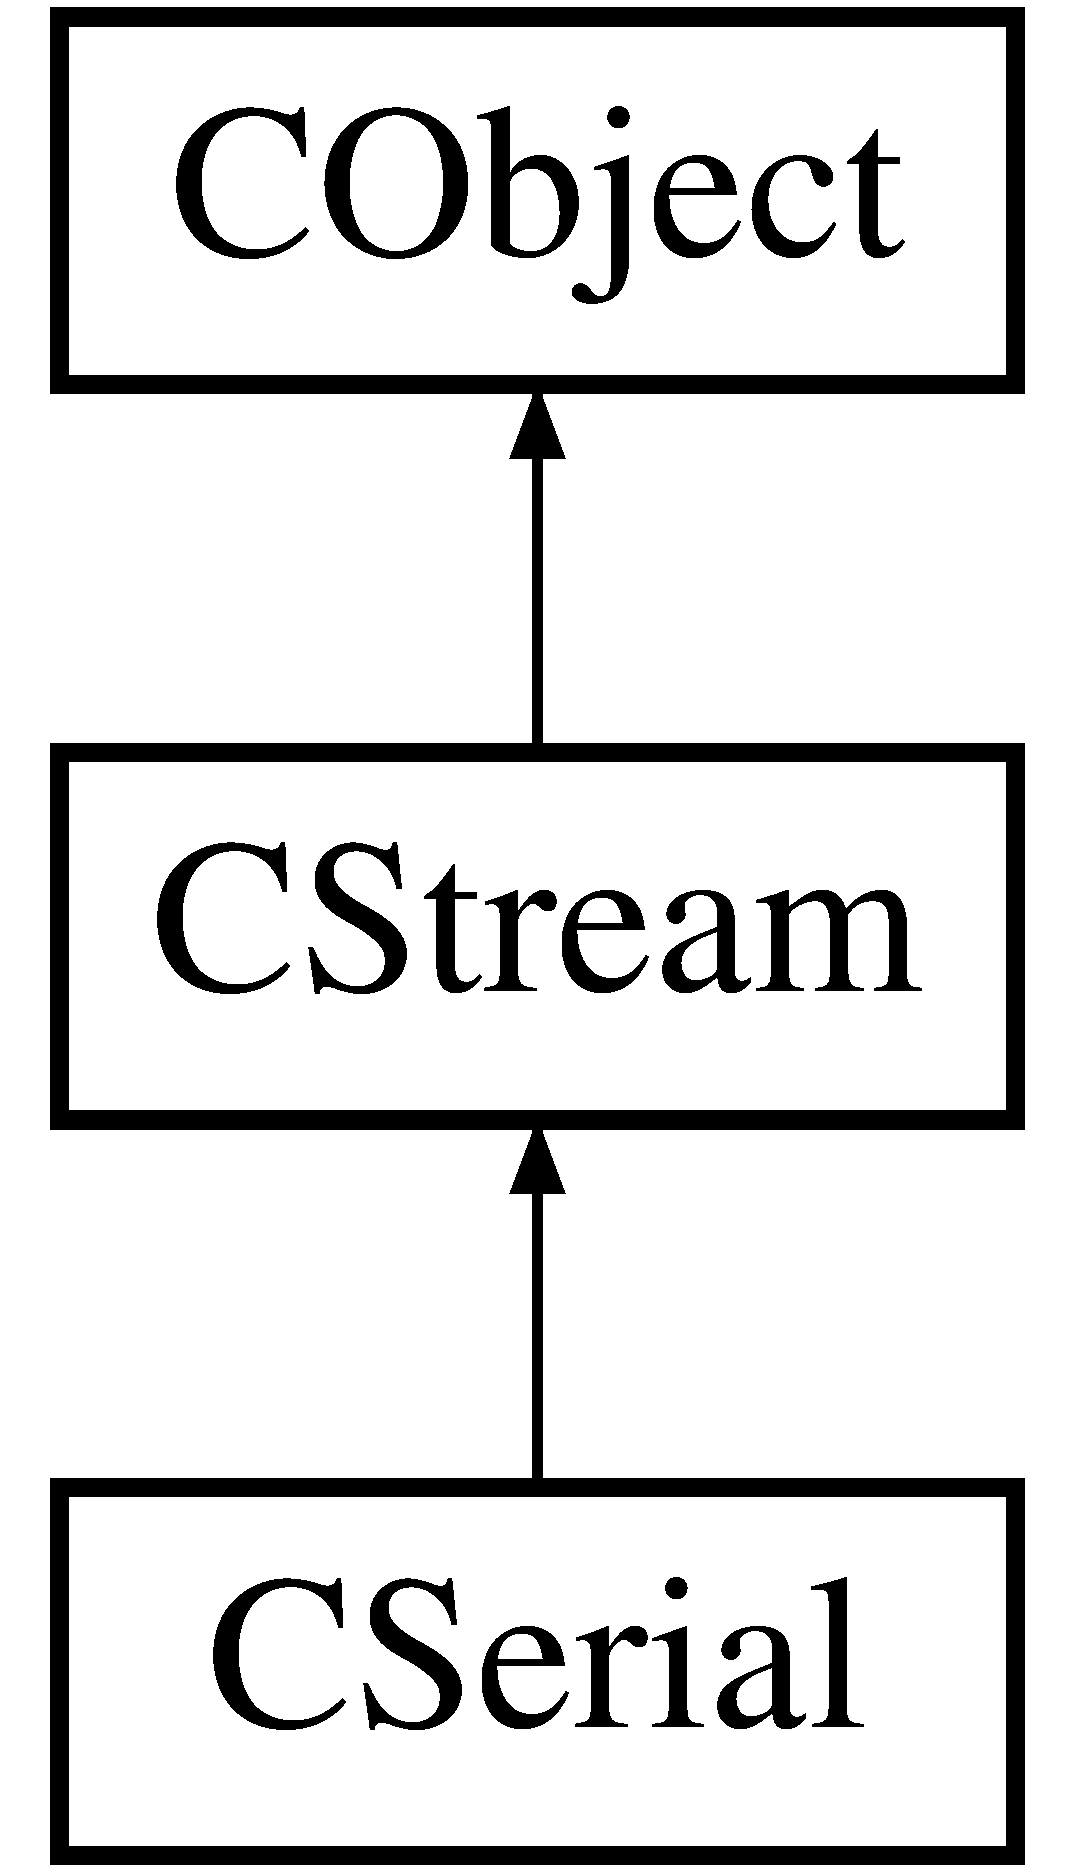
\includegraphics[height=3.000000cm]{d8/d1d/class_c_serial}
\end{center}
\end{figure}
\subsection*{Public Types}
\begin{DoxyCompactItemize}
\item 
enum \hyperlink{class_c_serial_ad38b0926868c6cfabb59e2da94f1cf40}{U\-A\-R\-T\-\_\-\-P\-A\-R\-I\-T\-Y\-\_\-\-T} \{ \\*
\hyperlink{class_c_serial_ad38b0926868c6cfabb59e2da94f1cf40a77e567bbd57497e51b0161ed1cd855a4}{U\-A\-R\-T\-\_\-\-P\-A\-R\-I\-T\-Y\-\_\-\-N\-O\-N\-E} = 4, 
\hyperlink{class_c_serial_ad38b0926868c6cfabb59e2da94f1cf40aa157a4ef710e04651e3aaf61a4d96ad9}{U\-A\-R\-T\-\_\-\-P\-A\-R\-I\-T\-Y\-\_\-\-O\-D\-D} = 0, 
\hyperlink{class_c_serial_ad38b0926868c6cfabb59e2da94f1cf40a4b7452e8ef848287eca86b7ea4411e65}{U\-A\-R\-T\-\_\-\-P\-A\-R\-I\-T\-Y\-\_\-\-E\-V\-E\-N} = 1, 
\hyperlink{class_c_serial_ad38b0926868c6cfabb59e2da94f1cf40a20c9bc3b3fa95b78898159cd2680e007}{U\-A\-R\-T\-\_\-\-P\-A\-R\-I\-T\-Y\-\_\-\-S\-P\-\_\-1} = 2, 
\\*
\hyperlink{class_c_serial_ad38b0926868c6cfabb59e2da94f1cf40a660aab6ba15f9c94cc9963ff226a77eb}{U\-A\-R\-T\-\_\-\-P\-A\-R\-I\-T\-Y\-\_\-\-S\-P\-\_\-0} = 3
 \}
\begin{DoxyCompactList}\small\item\em U\-A\-R\-T Parity type definitions. \end{DoxyCompactList}\item 
enum \hyperlink{class_c_serial_a628c8c9be04f0315c4dae70ce8ccc5b3}{U\-A\-R\-T\-\_\-\-D\-A\-T\-A\-B\-I\-T\-\_\-\-T} \{ \hyperlink{class_c_serial_a628c8c9be04f0315c4dae70ce8ccc5b3a7ac317a766becd83f58a2daa007fed1e}{U\-A\-R\-T\-\_\-\-D\-A\-T\-A\-B\-I\-T\-\_\-5} = 0, 
\hyperlink{class_c_serial_a628c8c9be04f0315c4dae70ce8ccc5b3a6c31f7e06c7a6779b6d72d37aba52fb1}{U\-A\-R\-T\-\_\-\-D\-A\-T\-A\-B\-I\-T\-\_\-6}, 
\hyperlink{class_c_serial_a628c8c9be04f0315c4dae70ce8ccc5b3abf533a46435efaddb8e38b9b9fe53eff}{U\-A\-R\-T\-\_\-\-D\-A\-T\-A\-B\-I\-T\-\_\-7}, 
\hyperlink{class_c_serial_a628c8c9be04f0315c4dae70ce8ccc5b3a196b716ca31d23301c1059b53ac35f25}{U\-A\-R\-T\-\_\-\-D\-A\-T\-A\-B\-I\-T\-\_\-8}
 \}
\begin{DoxyCompactList}\small\item\em U\-A\-R\-T Databit type definitions. \end{DoxyCompactList}\item 
enum \hyperlink{class_c_serial_af02af389f5596b7b40cf0d2ece57b04b}{U\-A\-R\-T\-\_\-\-S\-T\-O\-P\-B\-I\-T\-\_\-\-T} \{ \hyperlink{class_c_serial_af02af389f5596b7b40cf0d2ece57b04ba6351eeac6c2e865ed9019323e2491907}{U\-A\-R\-T\-\_\-\-S\-T\-O\-P\-B\-I\-T\-\_\-1} = (0), 
\hyperlink{class_c_serial_af02af389f5596b7b40cf0d2ece57b04bafe7ff299f68959471436234643298e71}{U\-A\-R\-T\-\_\-\-S\-T\-O\-P\-B\-I\-T\-\_\-2}
 \}
\begin{DoxyCompactList}\small\item\em U\-A\-R\-T Stop bit type definitions. \end{DoxyCompactList}\item 
enum \hyperlink{class_c_serial_a767bb157f0f469eb5bf5c99b8ada42f1}{U\-A\-R\-T\-\_\-\-F\-I\-T\-O\-\_\-\-L\-E\-V\-E\-L\-\_\-\-T} \{ \hyperlink{class_c_serial_a767bb157f0f469eb5bf5c99b8ada42f1aec8c4b69719ee6b1dc43cf6ccdd999de}{U\-A\-R\-T\-\_\-\-F\-I\-F\-O\-\_\-\-T\-R\-G\-L\-E\-V0} = 0, 
\hyperlink{class_c_serial_a767bb157f0f469eb5bf5c99b8ada42f1a2d29eb800e28d845f00b9fd5df1b955c}{U\-A\-R\-T\-\_\-\-F\-I\-F\-O\-\_\-\-T\-R\-G\-L\-E\-V1}, 
\hyperlink{class_c_serial_a767bb157f0f469eb5bf5c99b8ada42f1a3ca31e41f3d74e387b0ff625a927bcf4}{U\-A\-R\-T\-\_\-\-F\-I\-F\-O\-\_\-\-T\-R\-G\-L\-E\-V2}, 
\hyperlink{class_c_serial_a767bb157f0f469eb5bf5c99b8ada42f1a6893ab299c8d6be2e17efb39cd05e1a1}{U\-A\-R\-T\-\_\-\-F\-I\-F\-O\-\_\-\-T\-R\-G\-L\-E\-V3}
 \}
\begin{DoxyCompactList}\small\item\em R\-X F\-I\-F\-O Trigger Level type definitions. \end{DoxyCompactList}\end{DoxyCompactItemize}
\subsection*{Public Member Functions}
\begin{DoxyCompactItemize}
\item 
\hyperlink{class_c_serial_ad528b7355f527eabc415f6a8017745f4}{C\-Serial} (size\-\_\-t fifo\-\_\-size=32)
\item 
virtual void \hyperlink{class_c_serial_aff7c822bada51065ad52542fb9515be6}{enable} (uint32\-\_\-t baudrate, \hyperlink{class_c_serial_ad38b0926868c6cfabb59e2da94f1cf40}{U\-A\-R\-T\-\_\-\-P\-A\-R\-I\-T\-Y\-\_\-\-T} parity=\hyperlink{class_c_serial_ad38b0926868c6cfabb59e2da94f1cf40a77e567bbd57497e51b0161ed1cd855a4}{U\-A\-R\-T\-\_\-\-P\-A\-R\-I\-T\-Y\-\_\-\-N\-O\-N\-E}, \hyperlink{class_c_serial_a628c8c9be04f0315c4dae70ce8ccc5b3}{U\-A\-R\-T\-\_\-\-D\-A\-T\-A\-B\-I\-T\-\_\-\-T} databits=\hyperlink{class_c_serial_a628c8c9be04f0315c4dae70ce8ccc5b3a196b716ca31d23301c1059b53ac35f25}{U\-A\-R\-T\-\_\-\-D\-A\-T\-A\-B\-I\-T\-\_\-8}, \hyperlink{class_c_serial_af02af389f5596b7b40cf0d2ece57b04b}{U\-A\-R\-T\-\_\-\-S\-T\-O\-P\-B\-I\-T\-\_\-\-T} stopbits=\hyperlink{class_c_serial_af02af389f5596b7b40cf0d2ece57b04ba6351eeac6c2e865ed9019323e2491907}{U\-A\-R\-T\-\_\-\-S\-T\-O\-P\-B\-I\-T\-\_\-1}, \hyperlink{class_c_serial_a767bb157f0f469eb5bf5c99b8ada42f1}{U\-A\-R\-T\-\_\-\-F\-I\-T\-O\-\_\-\-L\-E\-V\-E\-L\-\_\-\-T} level=\hyperlink{class_c_serial_a767bb157f0f469eb5bf5c99b8ada42f1aec8c4b69719ee6b1dc43cf6ccdd999de}{U\-A\-R\-T\-\_\-\-F\-I\-F\-O\-\_\-\-T\-R\-G\-L\-E\-V0})
\item 
void \hyperlink{class_c_serial_a0c80ea521e310305579e787f21a55233}{settings} (uint32\-\_\-t baudrate, \hyperlink{class_c_serial_ad38b0926868c6cfabb59e2da94f1cf40}{U\-A\-R\-T\-\_\-\-P\-A\-R\-I\-T\-Y\-\_\-\-T} parity=\hyperlink{class_c_serial_ad38b0926868c6cfabb59e2da94f1cf40a77e567bbd57497e51b0161ed1cd855a4}{U\-A\-R\-T\-\_\-\-P\-A\-R\-I\-T\-Y\-\_\-\-N\-O\-N\-E}, \hyperlink{class_c_serial_a628c8c9be04f0315c4dae70ce8ccc5b3}{U\-A\-R\-T\-\_\-\-D\-A\-T\-A\-B\-I\-T\-\_\-\-T} databits=\hyperlink{class_c_serial_a628c8c9be04f0315c4dae70ce8ccc5b3a196b716ca31d23301c1059b53ac35f25}{U\-A\-R\-T\-\_\-\-D\-A\-T\-A\-B\-I\-T\-\_\-8}, \hyperlink{class_c_serial_af02af389f5596b7b40cf0d2ece57b04b}{U\-A\-R\-T\-\_\-\-S\-T\-O\-P\-B\-I\-T\-\_\-\-T} stopbits=\hyperlink{class_c_serial_af02af389f5596b7b40cf0d2ece57b04ba6351eeac6c2e865ed9019323e2491907}{U\-A\-R\-T\-\_\-\-S\-T\-O\-P\-B\-I\-T\-\_\-1}, \hyperlink{class_c_serial_a767bb157f0f469eb5bf5c99b8ada42f1}{U\-A\-R\-T\-\_\-\-F\-I\-T\-O\-\_\-\-L\-E\-V\-E\-L\-\_\-\-T} level=\hyperlink{class_c_serial_a767bb157f0f469eb5bf5c99b8ada42f1aec8c4b69719ee6b1dc43cf6ccdd999de}{U\-A\-R\-T\-\_\-\-F\-I\-F\-O\-\_\-\-T\-R\-G\-L\-E\-V0})
\item 
virtual int \hyperlink{class_c_serial_a0748723f610ddcfdc34286dbbfbd4917}{readable} ()
\item 
virtual int \hyperlink{class_c_serial_ac59cfe80216e1fb7eb479017f0bb8e7f}{writeable} ()
\item 
virtual int \hyperlink{class_c_serial_a9b658bf4bc4d81413627bc2fe81e1471}{read} (void $\ast$buf, int len, bool block=true)
\item 
virtual int \hyperlink{class_c_serial_adef6d3e77843c65617b7cb555c2f8732}{write} (const void $\ast$buf, int len, bool block=true)
\item 
virtual void \hyperlink{class_c_serial_a68aecf6351423ae0e8791870c9e694bf}{flush} ()
\item 
virtual void \hyperlink{class_c_serial_a678403bcefc3bd7dfc603c334383b8df}{begin} (uint32\-\_\-t speed)
\item 
virtual void \hyperlink{class_c_serial_a4fb5a06c1d1f746c834088c8beeb3097}{end} ()
\item 
virtual int \hyperlink{class_c_serial_a5c142221c0841e7c961e962c45bd2db7}{available} ()
\item 
virtual bool \hyperlink{class_c_serial_ae7c133c4586cd5ca729cd026f813a8a0}{is\-Connected} ()
\item 
void \hyperlink{class_c_serial_a9dc5498e6cae5a2d0d12cb57fc6ee335}{handshaking} ()
\end{DoxyCompactItemize}


\subsection{Detailed Description}
Use the \hyperlink{class_c_serial}{C\-Serial} class to transceiver the serial stream. 

\subsection{Member Enumeration Documentation}
\hypertarget{class_c_serial_ad38b0926868c6cfabb59e2da94f1cf40}{\index{C\-Serial@{C\-Serial}!U\-A\-R\-T\-\_\-\-P\-A\-R\-I\-T\-Y\-\_\-\-T@{U\-A\-R\-T\-\_\-\-P\-A\-R\-I\-T\-Y\-\_\-\-T}}
\index{U\-A\-R\-T\-\_\-\-P\-A\-R\-I\-T\-Y\-\_\-\-T@{U\-A\-R\-T\-\_\-\-P\-A\-R\-I\-T\-Y\-\_\-\-T}!CSerial@{C\-Serial}}
\subsubsection[{U\-A\-R\-T\-\_\-\-P\-A\-R\-I\-T\-Y\-\_\-\-T}]{\setlength{\rightskip}{0pt plus 5cm}enum {\bf C\-Serial\-::\-U\-A\-R\-T\-\_\-\-P\-A\-R\-I\-T\-Y\-\_\-\-T}}}\label{class_c_serial_ad38b0926868c6cfabb59e2da94f1cf40}


U\-A\-R\-T Parity type definitions. 

\begin{Desc}
\item[Enumerator]\par
\begin{description}
\index{U\-A\-R\-T\-\_\-\-P\-A\-R\-I\-T\-Y\-\_\-\-N\-O\-N\-E@{U\-A\-R\-T\-\_\-\-P\-A\-R\-I\-T\-Y\-\_\-\-N\-O\-N\-E}!C\-Serial@{C\-Serial}}\index{C\-Serial@{C\-Serial}!U\-A\-R\-T\-\_\-\-P\-A\-R\-I\-T\-Y\-\_\-\-N\-O\-N\-E@{U\-A\-R\-T\-\_\-\-P\-A\-R\-I\-T\-Y\-\_\-\-N\-O\-N\-E}}\item[{\em 
\hypertarget{class_c_serial_ad38b0926868c6cfabb59e2da94f1cf40a77e567bbd57497e51b0161ed1cd855a4}{U\-A\-R\-T\-\_\-\-P\-A\-R\-I\-T\-Y\-\_\-\-N\-O\-N\-E}\label{class_c_serial_ad38b0926868c6cfabb59e2da94f1cf40a77e567bbd57497e51b0161ed1cd855a4}
}]No parity \index{U\-A\-R\-T\-\_\-\-P\-A\-R\-I\-T\-Y\-\_\-\-O\-D\-D@{U\-A\-R\-T\-\_\-\-P\-A\-R\-I\-T\-Y\-\_\-\-O\-D\-D}!C\-Serial@{C\-Serial}}\index{C\-Serial@{C\-Serial}!U\-A\-R\-T\-\_\-\-P\-A\-R\-I\-T\-Y\-\_\-\-O\-D\-D@{U\-A\-R\-T\-\_\-\-P\-A\-R\-I\-T\-Y\-\_\-\-O\-D\-D}}\item[{\em 
\hypertarget{class_c_serial_ad38b0926868c6cfabb59e2da94f1cf40aa157a4ef710e04651e3aaf61a4d96ad9}{U\-A\-R\-T\-\_\-\-P\-A\-R\-I\-T\-Y\-\_\-\-O\-D\-D}\label{class_c_serial_ad38b0926868c6cfabb59e2da94f1cf40aa157a4ef710e04651e3aaf61a4d96ad9}
}]Odd parity \index{U\-A\-R\-T\-\_\-\-P\-A\-R\-I\-T\-Y\-\_\-\-E\-V\-E\-N@{U\-A\-R\-T\-\_\-\-P\-A\-R\-I\-T\-Y\-\_\-\-E\-V\-E\-N}!C\-Serial@{C\-Serial}}\index{C\-Serial@{C\-Serial}!U\-A\-R\-T\-\_\-\-P\-A\-R\-I\-T\-Y\-\_\-\-E\-V\-E\-N@{U\-A\-R\-T\-\_\-\-P\-A\-R\-I\-T\-Y\-\_\-\-E\-V\-E\-N}}\item[{\em 
\hypertarget{class_c_serial_ad38b0926868c6cfabb59e2da94f1cf40a4b7452e8ef848287eca86b7ea4411e65}{U\-A\-R\-T\-\_\-\-P\-A\-R\-I\-T\-Y\-\_\-\-E\-V\-E\-N}\label{class_c_serial_ad38b0926868c6cfabb59e2da94f1cf40a4b7452e8ef848287eca86b7ea4411e65}
}]Even parity \index{U\-A\-R\-T\-\_\-\-P\-A\-R\-I\-T\-Y\-\_\-\-S\-P\-\_\-1@{U\-A\-R\-T\-\_\-\-P\-A\-R\-I\-T\-Y\-\_\-\-S\-P\-\_\-1}!C\-Serial@{C\-Serial}}\index{C\-Serial@{C\-Serial}!U\-A\-R\-T\-\_\-\-P\-A\-R\-I\-T\-Y\-\_\-\-S\-P\-\_\-1@{U\-A\-R\-T\-\_\-\-P\-A\-R\-I\-T\-Y\-\_\-\-S\-P\-\_\-1}}\item[{\em 
\hypertarget{class_c_serial_ad38b0926868c6cfabb59e2da94f1cf40a20c9bc3b3fa95b78898159cd2680e007}{U\-A\-R\-T\-\_\-\-P\-A\-R\-I\-T\-Y\-\_\-\-S\-P\-\_\-1}\label{class_c_serial_ad38b0926868c6cfabb59e2da94f1cf40a20c9bc3b3fa95b78898159cd2680e007}
}]Forced \char`\"{}1\char`\"{} stick parity \index{U\-A\-R\-T\-\_\-\-P\-A\-R\-I\-T\-Y\-\_\-\-S\-P\-\_\-0@{U\-A\-R\-T\-\_\-\-P\-A\-R\-I\-T\-Y\-\_\-\-S\-P\-\_\-0}!C\-Serial@{C\-Serial}}\index{C\-Serial@{C\-Serial}!U\-A\-R\-T\-\_\-\-P\-A\-R\-I\-T\-Y\-\_\-\-S\-P\-\_\-0@{U\-A\-R\-T\-\_\-\-P\-A\-R\-I\-T\-Y\-\_\-\-S\-P\-\_\-0}}\item[{\em 
\hypertarget{class_c_serial_ad38b0926868c6cfabb59e2da94f1cf40a660aab6ba15f9c94cc9963ff226a77eb}{U\-A\-R\-T\-\_\-\-P\-A\-R\-I\-T\-Y\-\_\-\-S\-P\-\_\-0}\label{class_c_serial_ad38b0926868c6cfabb59e2da94f1cf40a660aab6ba15f9c94cc9963ff226a77eb}
}]Forced \char`\"{}0\char`\"{} stick parity \end{description}
\end{Desc}
\hypertarget{class_c_serial_a628c8c9be04f0315c4dae70ce8ccc5b3}{\index{C\-Serial@{C\-Serial}!U\-A\-R\-T\-\_\-\-D\-A\-T\-A\-B\-I\-T\-\_\-\-T@{U\-A\-R\-T\-\_\-\-D\-A\-T\-A\-B\-I\-T\-\_\-\-T}}
\index{U\-A\-R\-T\-\_\-\-D\-A\-T\-A\-B\-I\-T\-\_\-\-T@{U\-A\-R\-T\-\_\-\-D\-A\-T\-A\-B\-I\-T\-\_\-\-T}!CSerial@{C\-Serial}}
\subsubsection[{U\-A\-R\-T\-\_\-\-D\-A\-T\-A\-B\-I\-T\-\_\-\-T}]{\setlength{\rightskip}{0pt plus 5cm}enum {\bf C\-Serial\-::\-U\-A\-R\-T\-\_\-\-D\-A\-T\-A\-B\-I\-T\-\_\-\-T}}}\label{class_c_serial_a628c8c9be04f0315c4dae70ce8ccc5b3}


U\-A\-R\-T Databit type definitions. 

\begin{Desc}
\item[Enumerator]\par
\begin{description}
\index{U\-A\-R\-T\-\_\-\-D\-A\-T\-A\-B\-I\-T\-\_\-5@{U\-A\-R\-T\-\_\-\-D\-A\-T\-A\-B\-I\-T\-\_\-5}!C\-Serial@{C\-Serial}}\index{C\-Serial@{C\-Serial}!U\-A\-R\-T\-\_\-\-D\-A\-T\-A\-B\-I\-T\-\_\-5@{U\-A\-R\-T\-\_\-\-D\-A\-T\-A\-B\-I\-T\-\_\-5}}\item[{\em 
\hypertarget{class_c_serial_a628c8c9be04f0315c4dae70ce8ccc5b3a7ac317a766becd83f58a2daa007fed1e}{U\-A\-R\-T\-\_\-\-D\-A\-T\-A\-B\-I\-T\-\_\-5}\label{class_c_serial_a628c8c9be04f0315c4dae70ce8ccc5b3a7ac317a766becd83f58a2daa007fed1e}
}]U\-A\-R\-T 5 bit data mode \index{U\-A\-R\-T\-\_\-\-D\-A\-T\-A\-B\-I\-T\-\_\-6@{U\-A\-R\-T\-\_\-\-D\-A\-T\-A\-B\-I\-T\-\_\-6}!C\-Serial@{C\-Serial}}\index{C\-Serial@{C\-Serial}!U\-A\-R\-T\-\_\-\-D\-A\-T\-A\-B\-I\-T\-\_\-6@{U\-A\-R\-T\-\_\-\-D\-A\-T\-A\-B\-I\-T\-\_\-6}}\item[{\em 
\hypertarget{class_c_serial_a628c8c9be04f0315c4dae70ce8ccc5b3a6c31f7e06c7a6779b6d72d37aba52fb1}{U\-A\-R\-T\-\_\-\-D\-A\-T\-A\-B\-I\-T\-\_\-6}\label{class_c_serial_a628c8c9be04f0315c4dae70ce8ccc5b3a6c31f7e06c7a6779b6d72d37aba52fb1}
}]U\-A\-R\-T 6 bit data mode \index{U\-A\-R\-T\-\_\-\-D\-A\-T\-A\-B\-I\-T\-\_\-7@{U\-A\-R\-T\-\_\-\-D\-A\-T\-A\-B\-I\-T\-\_\-7}!C\-Serial@{C\-Serial}}\index{C\-Serial@{C\-Serial}!U\-A\-R\-T\-\_\-\-D\-A\-T\-A\-B\-I\-T\-\_\-7@{U\-A\-R\-T\-\_\-\-D\-A\-T\-A\-B\-I\-T\-\_\-7}}\item[{\em 
\hypertarget{class_c_serial_a628c8c9be04f0315c4dae70ce8ccc5b3abf533a46435efaddb8e38b9b9fe53eff}{U\-A\-R\-T\-\_\-\-D\-A\-T\-A\-B\-I\-T\-\_\-7}\label{class_c_serial_a628c8c9be04f0315c4dae70ce8ccc5b3abf533a46435efaddb8e38b9b9fe53eff}
}]U\-A\-R\-T 7 bit data mode \index{U\-A\-R\-T\-\_\-\-D\-A\-T\-A\-B\-I\-T\-\_\-8@{U\-A\-R\-T\-\_\-\-D\-A\-T\-A\-B\-I\-T\-\_\-8}!C\-Serial@{C\-Serial}}\index{C\-Serial@{C\-Serial}!U\-A\-R\-T\-\_\-\-D\-A\-T\-A\-B\-I\-T\-\_\-8@{U\-A\-R\-T\-\_\-\-D\-A\-T\-A\-B\-I\-T\-\_\-8}}\item[{\em 
\hypertarget{class_c_serial_a628c8c9be04f0315c4dae70ce8ccc5b3a196b716ca31d23301c1059b53ac35f25}{U\-A\-R\-T\-\_\-\-D\-A\-T\-A\-B\-I\-T\-\_\-8}\label{class_c_serial_a628c8c9be04f0315c4dae70ce8ccc5b3a196b716ca31d23301c1059b53ac35f25}
}]U\-A\-R\-T 8 bit data mode \end{description}
\end{Desc}
\hypertarget{class_c_serial_af02af389f5596b7b40cf0d2ece57b04b}{\index{C\-Serial@{C\-Serial}!U\-A\-R\-T\-\_\-\-S\-T\-O\-P\-B\-I\-T\-\_\-\-T@{U\-A\-R\-T\-\_\-\-S\-T\-O\-P\-B\-I\-T\-\_\-\-T}}
\index{U\-A\-R\-T\-\_\-\-S\-T\-O\-P\-B\-I\-T\-\_\-\-T@{U\-A\-R\-T\-\_\-\-S\-T\-O\-P\-B\-I\-T\-\_\-\-T}!CSerial@{C\-Serial}}
\subsubsection[{U\-A\-R\-T\-\_\-\-S\-T\-O\-P\-B\-I\-T\-\_\-\-T}]{\setlength{\rightskip}{0pt plus 5cm}enum {\bf C\-Serial\-::\-U\-A\-R\-T\-\_\-\-S\-T\-O\-P\-B\-I\-T\-\_\-\-T}}}\label{class_c_serial_af02af389f5596b7b40cf0d2ece57b04b}


U\-A\-R\-T Stop bit type definitions. 

\begin{Desc}
\item[Enumerator]\par
\begin{description}
\index{U\-A\-R\-T\-\_\-\-S\-T\-O\-P\-B\-I\-T\-\_\-1@{U\-A\-R\-T\-\_\-\-S\-T\-O\-P\-B\-I\-T\-\_\-1}!C\-Serial@{C\-Serial}}\index{C\-Serial@{C\-Serial}!U\-A\-R\-T\-\_\-\-S\-T\-O\-P\-B\-I\-T\-\_\-1@{U\-A\-R\-T\-\_\-\-S\-T\-O\-P\-B\-I\-T\-\_\-1}}\item[{\em 
\hypertarget{class_c_serial_af02af389f5596b7b40cf0d2ece57b04ba6351eeac6c2e865ed9019323e2491907}{U\-A\-R\-T\-\_\-\-S\-T\-O\-P\-B\-I\-T\-\_\-1}\label{class_c_serial_af02af389f5596b7b40cf0d2ece57b04ba6351eeac6c2e865ed9019323e2491907}
}]U\-A\-R\-T 1 Stop Bits Select \index{U\-A\-R\-T\-\_\-\-S\-T\-O\-P\-B\-I\-T\-\_\-2@{U\-A\-R\-T\-\_\-\-S\-T\-O\-P\-B\-I\-T\-\_\-2}!C\-Serial@{C\-Serial}}\index{C\-Serial@{C\-Serial}!U\-A\-R\-T\-\_\-\-S\-T\-O\-P\-B\-I\-T\-\_\-2@{U\-A\-R\-T\-\_\-\-S\-T\-O\-P\-B\-I\-T\-\_\-2}}\item[{\em 
\hypertarget{class_c_serial_af02af389f5596b7b40cf0d2ece57b04bafe7ff299f68959471436234643298e71}{U\-A\-R\-T\-\_\-\-S\-T\-O\-P\-B\-I\-T\-\_\-2}\label{class_c_serial_af02af389f5596b7b40cf0d2ece57b04bafe7ff299f68959471436234643298e71}
}]U\-A\-R\-T Two Stop Bits Select \end{description}
\end{Desc}
\hypertarget{class_c_serial_a767bb157f0f469eb5bf5c99b8ada42f1}{\index{C\-Serial@{C\-Serial}!U\-A\-R\-T\-\_\-\-F\-I\-T\-O\-\_\-\-L\-E\-V\-E\-L\-\_\-\-T@{U\-A\-R\-T\-\_\-\-F\-I\-T\-O\-\_\-\-L\-E\-V\-E\-L\-\_\-\-T}}
\index{U\-A\-R\-T\-\_\-\-F\-I\-T\-O\-\_\-\-L\-E\-V\-E\-L\-\_\-\-T@{U\-A\-R\-T\-\_\-\-F\-I\-T\-O\-\_\-\-L\-E\-V\-E\-L\-\_\-\-T}!CSerial@{C\-Serial}}
\subsubsection[{U\-A\-R\-T\-\_\-\-F\-I\-T\-O\-\_\-\-L\-E\-V\-E\-L\-\_\-\-T}]{\setlength{\rightskip}{0pt plus 5cm}enum {\bf C\-Serial\-::\-U\-A\-R\-T\-\_\-\-F\-I\-T\-O\-\_\-\-L\-E\-V\-E\-L\-\_\-\-T}}}\label{class_c_serial_a767bb157f0f469eb5bf5c99b8ada42f1}


R\-X F\-I\-F\-O Trigger Level type definitions. 

\begin{Desc}
\item[Enumerator]\par
\begin{description}
\index{U\-A\-R\-T\-\_\-\-F\-I\-F\-O\-\_\-\-T\-R\-G\-L\-E\-V0@{U\-A\-R\-T\-\_\-\-F\-I\-F\-O\-\_\-\-T\-R\-G\-L\-E\-V0}!C\-Serial@{C\-Serial}}\index{C\-Serial@{C\-Serial}!U\-A\-R\-T\-\_\-\-F\-I\-F\-O\-\_\-\-T\-R\-G\-L\-E\-V0@{U\-A\-R\-T\-\_\-\-F\-I\-F\-O\-\_\-\-T\-R\-G\-L\-E\-V0}}\item[{\em 
\hypertarget{class_c_serial_a767bb157f0f469eb5bf5c99b8ada42f1aec8c4b69719ee6b1dc43cf6ccdd999de}{U\-A\-R\-T\-\_\-\-F\-I\-F\-O\-\_\-\-T\-R\-G\-L\-E\-V0}\label{class_c_serial_a767bb157f0f469eb5bf5c99b8ada42f1aec8c4b69719ee6b1dc43cf6ccdd999de}
}]U\-A\-R\-T F\-I\-F\-O trigger level 0\-: 1 character \index{U\-A\-R\-T\-\_\-\-F\-I\-F\-O\-\_\-\-T\-R\-G\-L\-E\-V1@{U\-A\-R\-T\-\_\-\-F\-I\-F\-O\-\_\-\-T\-R\-G\-L\-E\-V1}!C\-Serial@{C\-Serial}}\index{C\-Serial@{C\-Serial}!U\-A\-R\-T\-\_\-\-F\-I\-F\-O\-\_\-\-T\-R\-G\-L\-E\-V1@{U\-A\-R\-T\-\_\-\-F\-I\-F\-O\-\_\-\-T\-R\-G\-L\-E\-V1}}\item[{\em 
\hypertarget{class_c_serial_a767bb157f0f469eb5bf5c99b8ada42f1a2d29eb800e28d845f00b9fd5df1b955c}{U\-A\-R\-T\-\_\-\-F\-I\-F\-O\-\_\-\-T\-R\-G\-L\-E\-V1}\label{class_c_serial_a767bb157f0f469eb5bf5c99b8ada42f1a2d29eb800e28d845f00b9fd5df1b955c}
}]U\-A\-R\-T F\-I\-F\-O trigger level 1\-: 4 character \index{U\-A\-R\-T\-\_\-\-F\-I\-F\-O\-\_\-\-T\-R\-G\-L\-E\-V2@{U\-A\-R\-T\-\_\-\-F\-I\-F\-O\-\_\-\-T\-R\-G\-L\-E\-V2}!C\-Serial@{C\-Serial}}\index{C\-Serial@{C\-Serial}!U\-A\-R\-T\-\_\-\-F\-I\-F\-O\-\_\-\-T\-R\-G\-L\-E\-V2@{U\-A\-R\-T\-\_\-\-F\-I\-F\-O\-\_\-\-T\-R\-G\-L\-E\-V2}}\item[{\em 
\hypertarget{class_c_serial_a767bb157f0f469eb5bf5c99b8ada42f1a3ca31e41f3d74e387b0ff625a927bcf4}{U\-A\-R\-T\-\_\-\-F\-I\-F\-O\-\_\-\-T\-R\-G\-L\-E\-V2}\label{class_c_serial_a767bb157f0f469eb5bf5c99b8ada42f1a3ca31e41f3d74e387b0ff625a927bcf4}
}]U\-A\-R\-T F\-I\-F\-O trigger level 2\-: 8 character \index{U\-A\-R\-T\-\_\-\-F\-I\-F\-O\-\_\-\-T\-R\-G\-L\-E\-V3@{U\-A\-R\-T\-\_\-\-F\-I\-F\-O\-\_\-\-T\-R\-G\-L\-E\-V3}!C\-Serial@{C\-Serial}}\index{C\-Serial@{C\-Serial}!U\-A\-R\-T\-\_\-\-F\-I\-F\-O\-\_\-\-T\-R\-G\-L\-E\-V3@{U\-A\-R\-T\-\_\-\-F\-I\-F\-O\-\_\-\-T\-R\-G\-L\-E\-V3}}\item[{\em 
\hypertarget{class_c_serial_a767bb157f0f469eb5bf5c99b8ada42f1a6893ab299c8d6be2e17efb39cd05e1a1}{U\-A\-R\-T\-\_\-\-F\-I\-F\-O\-\_\-\-T\-R\-G\-L\-E\-V3}\label{class_c_serial_a767bb157f0f469eb5bf5c99b8ada42f1a6893ab299c8d6be2e17efb39cd05e1a1}
}]U\-A\-R\-T F\-I\-F\-O trigger level 3\-: 14 character \end{description}
\end{Desc}


\subsection{Constructor \& Destructor Documentation}
\hypertarget{class_c_serial_ad528b7355f527eabc415f6a8017745f4}{\index{C\-Serial@{C\-Serial}!C\-Serial@{C\-Serial}}
\index{C\-Serial@{C\-Serial}!CSerial@{C\-Serial}}
\subsubsection[{C\-Serial}]{\setlength{\rightskip}{0pt plus 5cm}C\-Serial\-::\-C\-Serial (
\begin{DoxyParamCaption}
\item[{size\-\_\-t}]{fifo\-\_\-size = {\ttfamily 32}}
\end{DoxyParamCaption}
)}}\label{class_c_serial_ad528b7355f527eabc415f6a8017745f4}
Constructs a \hyperlink{class_c_serial}{C\-Serial} object. 
\begin{DoxyParams}{Parameters}
{\em fifo\-\_\-size} & \\
\hline
\end{DoxyParams}


\subsection{Member Function Documentation}
\hypertarget{class_c_serial_aff7c822bada51065ad52542fb9515be6}{\index{C\-Serial@{C\-Serial}!enable@{enable}}
\index{enable@{enable}!CSerial@{C\-Serial}}
\subsubsection[{enable}]{\setlength{\rightskip}{0pt plus 5cm}virtual void C\-Serial\-::enable (
\begin{DoxyParamCaption}
\item[{uint32\-\_\-t}]{baudrate, }
\item[{{\bf U\-A\-R\-T\-\_\-\-P\-A\-R\-I\-T\-Y\-\_\-\-T}}]{parity = {\ttfamily {\bf U\-A\-R\-T\-\_\-\-P\-A\-R\-I\-T\-Y\-\_\-\-N\-O\-N\-E}}, }
\item[{{\bf U\-A\-R\-T\-\_\-\-D\-A\-T\-A\-B\-I\-T\-\_\-\-T}}]{databits = {\ttfamily {\bf U\-A\-R\-T\-\_\-\-D\-A\-T\-A\-B\-I\-T\-\_\-8}}, }
\item[{{\bf U\-A\-R\-T\-\_\-\-S\-T\-O\-P\-B\-I\-T\-\_\-\-T}}]{stopbits = {\ttfamily {\bf U\-A\-R\-T\-\_\-\-S\-T\-O\-P\-B\-I\-T\-\_\-1}}, }
\item[{{\bf U\-A\-R\-T\-\_\-\-F\-I\-T\-O\-\_\-\-L\-E\-V\-E\-L\-\_\-\-T}}]{level = {\ttfamily {\bf U\-A\-R\-T\-\_\-\-F\-I\-F\-O\-\_\-\-T\-R\-G\-L\-E\-V0}}}
\end{DoxyParamCaption}
)\hspace{0.3cm}{\ttfamily [virtual]}}}\label{class_c_serial_aff7c822bada51065ad52542fb9515be6}
Call the member function to enable the serial port. 
\begin{DoxyParams}{Parameters}
{\em baudrate} & is a unsigned long integer to specified the data baud-\/rate. \\
\hline
{\em parity} & is an U\-A\-R\-T\-\_\-\-P\-A\-R\-I\-T\-Y\-\_\-\-T enumerations. \\
\hline
{\em databits} & is an U\-A\-R\-T\-\_\-\-D\-A\-T\-A\-B\-I\-T\-\_\-\-T enumerations. \\
\hline
{\em stopbits} & is an U\-A\-R\-T\-\_\-\-S\-T\-O\-P\-B\-I\-T\-\_\-\-T enumerations. \\
\hline
{\em level} & is U\-A\-R\-T\-\_\-\-F\-I\-T\-O\-\_\-\-L\-E\-V\-E\-L\-\_\-\-T to trigger how many receiver U\-A\-R\-Tn F\-I\-F\-O characters must be written before an interrupt or D\-M\-A request is activated. \\
\hline
\end{DoxyParams}
\hypertarget{class_c_serial_a0c80ea521e310305579e787f21a55233}{\index{C\-Serial@{C\-Serial}!settings@{settings}}
\index{settings@{settings}!CSerial@{C\-Serial}}
\subsubsection[{settings}]{\setlength{\rightskip}{0pt plus 5cm}void C\-Serial\-::settings (
\begin{DoxyParamCaption}
\item[{uint32\-\_\-t}]{baudrate, }
\item[{{\bf U\-A\-R\-T\-\_\-\-P\-A\-R\-I\-T\-Y\-\_\-\-T}}]{parity = {\ttfamily {\bf U\-A\-R\-T\-\_\-\-P\-A\-R\-I\-T\-Y\-\_\-\-N\-O\-N\-E}}, }
\item[{{\bf U\-A\-R\-T\-\_\-\-D\-A\-T\-A\-B\-I\-T\-\_\-\-T}}]{databits = {\ttfamily {\bf U\-A\-R\-T\-\_\-\-D\-A\-T\-A\-B\-I\-T\-\_\-8}}, }
\item[{{\bf U\-A\-R\-T\-\_\-\-S\-T\-O\-P\-B\-I\-T\-\_\-\-T}}]{stopbits = {\ttfamily {\bf U\-A\-R\-T\-\_\-\-S\-T\-O\-P\-B\-I\-T\-\_\-1}}, }
\item[{{\bf U\-A\-R\-T\-\_\-\-F\-I\-T\-O\-\_\-\-L\-E\-V\-E\-L\-\_\-\-T}}]{level = {\ttfamily {\bf U\-A\-R\-T\-\_\-\-F\-I\-F\-O\-\_\-\-T\-R\-G\-L\-E\-V0}}}
\end{DoxyParamCaption}
)\hspace{0.3cm}{\ttfamily [inline]}}}\label{class_c_serial_a0c80ea521e310305579e787f21a55233}
Outmoded, redirect to \hyperlink{class_c_serial_aff7c822bada51065ad52542fb9515be6}{enable()} \hypertarget{class_c_serial_a0748723f610ddcfdc34286dbbfbd4917}{\index{C\-Serial@{C\-Serial}!readable@{readable}}
\index{readable@{readable}!CSerial@{C\-Serial}}
\subsubsection[{readable}]{\setlength{\rightskip}{0pt plus 5cm}virtual int C\-Serial\-::readable (
\begin{DoxyParamCaption}
{}
\end{DoxyParamCaption}
)\hspace{0.3cm}{\ttfamily [virtual]}}}\label{class_c_serial_a0748723f610ddcfdc34286dbbfbd4917}
Call the member function to check that receive buffer is ready to read. \begin{DoxyReturn}{Returns}
greater than zero if receive data from serial port. 
\end{DoxyReturn}


Reimplemented from \hyperlink{class_c_stream_a96328807241e15017868b845b06fd9e4}{C\-Stream}.

\hypertarget{class_c_serial_ac59cfe80216e1fb7eb479017f0bb8e7f}{\index{C\-Serial@{C\-Serial}!writeable@{writeable}}
\index{writeable@{writeable}!CSerial@{C\-Serial}}
\subsubsection[{writeable}]{\setlength{\rightskip}{0pt plus 5cm}virtual int C\-Serial\-::writeable (
\begin{DoxyParamCaption}
{}
\end{DoxyParamCaption}
)\hspace{0.3cm}{\ttfamily [virtual]}}}\label{class_c_serial_ac59cfe80216e1fb7eb479017f0bb8e7f}
Call the member function to check that transmit buffer is ready to write. \begin{DoxyReturn}{Returns}
how many bytes can be write to transmit buffer. 
\end{DoxyReturn}


Reimplemented from \hyperlink{class_c_stream_a56ec27ee664f1a4eb9910988b78833d5}{C\-Stream}.

\hypertarget{class_c_serial_a9b658bf4bc4d81413627bc2fe81e1471}{\index{C\-Serial@{C\-Serial}!read@{read}}
\index{read@{read}!CSerial@{C\-Serial}}
\subsubsection[{read}]{\setlength{\rightskip}{0pt plus 5cm}virtual int C\-Serial\-::read (
\begin{DoxyParamCaption}
\item[{void $\ast$}]{buf, }
\item[{int}]{len, }
\item[{bool}]{block = {\ttfamily true}}
\end{DoxyParamCaption}
)\hspace{0.3cm}{\ttfamily [virtual]}}}\label{class_c_serial_a9b658bf4bc4d81413627bc2fe81e1471}
Call the member function to read a data block from serial port. 
\begin{DoxyParams}[1]{Parameters}
\mbox{\tt out}  & {\em buf} & is a pointer which contain the data block from serial port. \\
\hline
\mbox{\tt in}  & {\em len} & is a integer to specified the buffer length. \\
\hline
\mbox{\tt in}  & {\em block} & is a boolean value to specified to wait for reading. \\
\hline
\end{DoxyParams}


Reimplemented from \hyperlink{class_c_stream_a80977482ffb2f7b626a9f29f437b7d8d}{C\-Stream}.

\hypertarget{class_c_serial_adef6d3e77843c65617b7cb555c2f8732}{\index{C\-Serial@{C\-Serial}!write@{write}}
\index{write@{write}!CSerial@{C\-Serial}}
\subsubsection[{write}]{\setlength{\rightskip}{0pt plus 5cm}virtual int C\-Serial\-::write (
\begin{DoxyParamCaption}
\item[{const void $\ast$}]{buf, }
\item[{int}]{len, }
\item[{bool}]{block = {\ttfamily true}}
\end{DoxyParamCaption}
)\hspace{0.3cm}{\ttfamily [virtual]}}}\label{class_c_serial_adef6d3e77843c65617b7cb555c2f8732}
Call the member function to write a data block to serial port 
\begin{DoxyParams}[1]{Parameters}
\mbox{\tt in}  & {\em buf} & is a pointer which data block want to send to serial port. \\
\hline
\mbox{\tt in}  & {\em len} & is a integer value to specified the buffer length. \\
\hline
\mbox{\tt in}  & {\em block} & is a boolean value to specified to wait for writing. \\
\hline
\end{DoxyParams}


Reimplemented from \hyperlink{class_c_stream_a172fe857c74488b881007c65cc2e9552}{C\-Stream}.

\hypertarget{class_c_serial_a68aecf6351423ae0e8791870c9e694bf}{\index{C\-Serial@{C\-Serial}!flush@{flush}}
\index{flush@{flush}!CSerial@{C\-Serial}}
\subsubsection[{flush}]{\setlength{\rightskip}{0pt plus 5cm}virtual void C\-Serial\-::flush (
\begin{DoxyParamCaption}
{}
\end{DoxyParamCaption}
)\hspace{0.3cm}{\ttfamily [virtual]}}}\label{class_c_serial_a68aecf6351423ae0e8791870c9e694bf}
Call the member function to wait for transmission of outgoing serial data to complete. 

Reimplemented from \hyperlink{class_c_stream_a5bd707b33627e01c2069b14bbf10694a}{C\-Stream}.

\hypertarget{class_c_serial_a678403bcefc3bd7dfc603c334383b8df}{\index{C\-Serial@{C\-Serial}!begin@{begin}}
\index{begin@{begin}!CSerial@{C\-Serial}}
\subsubsection[{begin}]{\setlength{\rightskip}{0pt plus 5cm}virtual void C\-Serial\-::begin (
\begin{DoxyParamCaption}
\item[{uint32\-\_\-t}]{speed}
\end{DoxyParamCaption}
)\hspace{0.3cm}{\ttfamily [inline]}, {\ttfamily [virtual]}}}\label{class_c_serial_a678403bcefc3bd7dfc603c334383b8df}
Call the member function to begin the serial port. \begin{DoxyNote}{Note}
The 'begin' is an inline code to call the exist \hyperlink{class_c_serial_a0c80ea521e310305579e787f21a55233}{settings()} member function. 
\end{DoxyNote}
\hypertarget{class_c_serial_a4fb5a06c1d1f746c834088c8beeb3097}{\index{C\-Serial@{C\-Serial}!end@{end}}
\index{end@{end}!CSerial@{C\-Serial}}
\subsubsection[{end}]{\setlength{\rightskip}{0pt plus 5cm}virtual void C\-Serial\-::end (
\begin{DoxyParamCaption}
{}
\end{DoxyParamCaption}
)\hspace{0.3cm}{\ttfamily [inline]}, {\ttfamily [virtual]}}}\label{class_c_serial_a4fb5a06c1d1f746c834088c8beeb3097}
Call the member function to end the serial port. \hypertarget{class_c_serial_a5c142221c0841e7c961e962c45bd2db7}{\index{C\-Serial@{C\-Serial}!available@{available}}
\index{available@{available}!CSerial@{C\-Serial}}
\subsubsection[{available}]{\setlength{\rightskip}{0pt plus 5cm}virtual int C\-Serial\-::available (
\begin{DoxyParamCaption}
{}
\end{DoxyParamCaption}
)\hspace{0.3cm}{\ttfamily [inline]}, {\ttfamily [virtual]}}}\label{class_c_serial_a5c142221c0841e7c961e962c45bd2db7}
Call the member function to check that receive buffer is ready. \begin{DoxyNote}{Note}
The 'available' is an inline code to call the exist \hyperlink{class_c_serial_a0748723f610ddcfdc34286dbbfbd4917}{readable()} member function. 
\end{DoxyNote}
\hypertarget{class_c_serial_ae7c133c4586cd5ca729cd026f813a8a0}{\index{C\-Serial@{C\-Serial}!is\-Connected@{is\-Connected}}
\index{is\-Connected@{is\-Connected}!CSerial@{C\-Serial}}
\subsubsection[{is\-Connected}]{\setlength{\rightskip}{0pt plus 5cm}virtual bool C\-Serial\-::is\-Connected (
\begin{DoxyParamCaption}
{}
\end{DoxyParamCaption}
)\hspace{0.3cm}{\ttfamily [inline]}, {\ttfamily [virtual]}}}\label{class_c_serial_ae7c133c4586cd5ca729cd026f813a8a0}
Call the member function to check that serial port is ready. 

Reimplemented from \hyperlink{class_c_stream_a7a152e6bda8654064634428d81bd81cb}{C\-Stream}.

\hypertarget{class_c_serial_a9dc5498e6cae5a2d0d12cb57fc6ee335}{\index{C\-Serial@{C\-Serial}!handshaking@{handshaking}}
\index{handshaking@{handshaking}!CSerial@{C\-Serial}}
\subsubsection[{handshaking}]{\setlength{\rightskip}{0pt plus 5cm}void C\-Serial\-::handshaking (
\begin{DoxyParamCaption}
{}
\end{DoxyParamCaption}
)}}\label{class_c_serial_a9dc5498e6cae5a2d0d12cb57fc6ee335}
Enable hardware handshaking R\-T\-S/\-C\-T\-S pins 

The documentation for this class was generated from the following file\-:\begin{DoxyCompactItemize}
\item 
serial.\-h\end{DoxyCompactItemize}

\hypertarget{class_c_shell}{\section{C\-Shell Class Reference}
\label{class_c_shell}\index{C\-Shell@{C\-Shell}}
}


{\ttfamily \#include $<$shell.\-h$>$}

Inheritance diagram for C\-Shell\-:\begin{figure}[H]
\begin{center}
\leavevmode
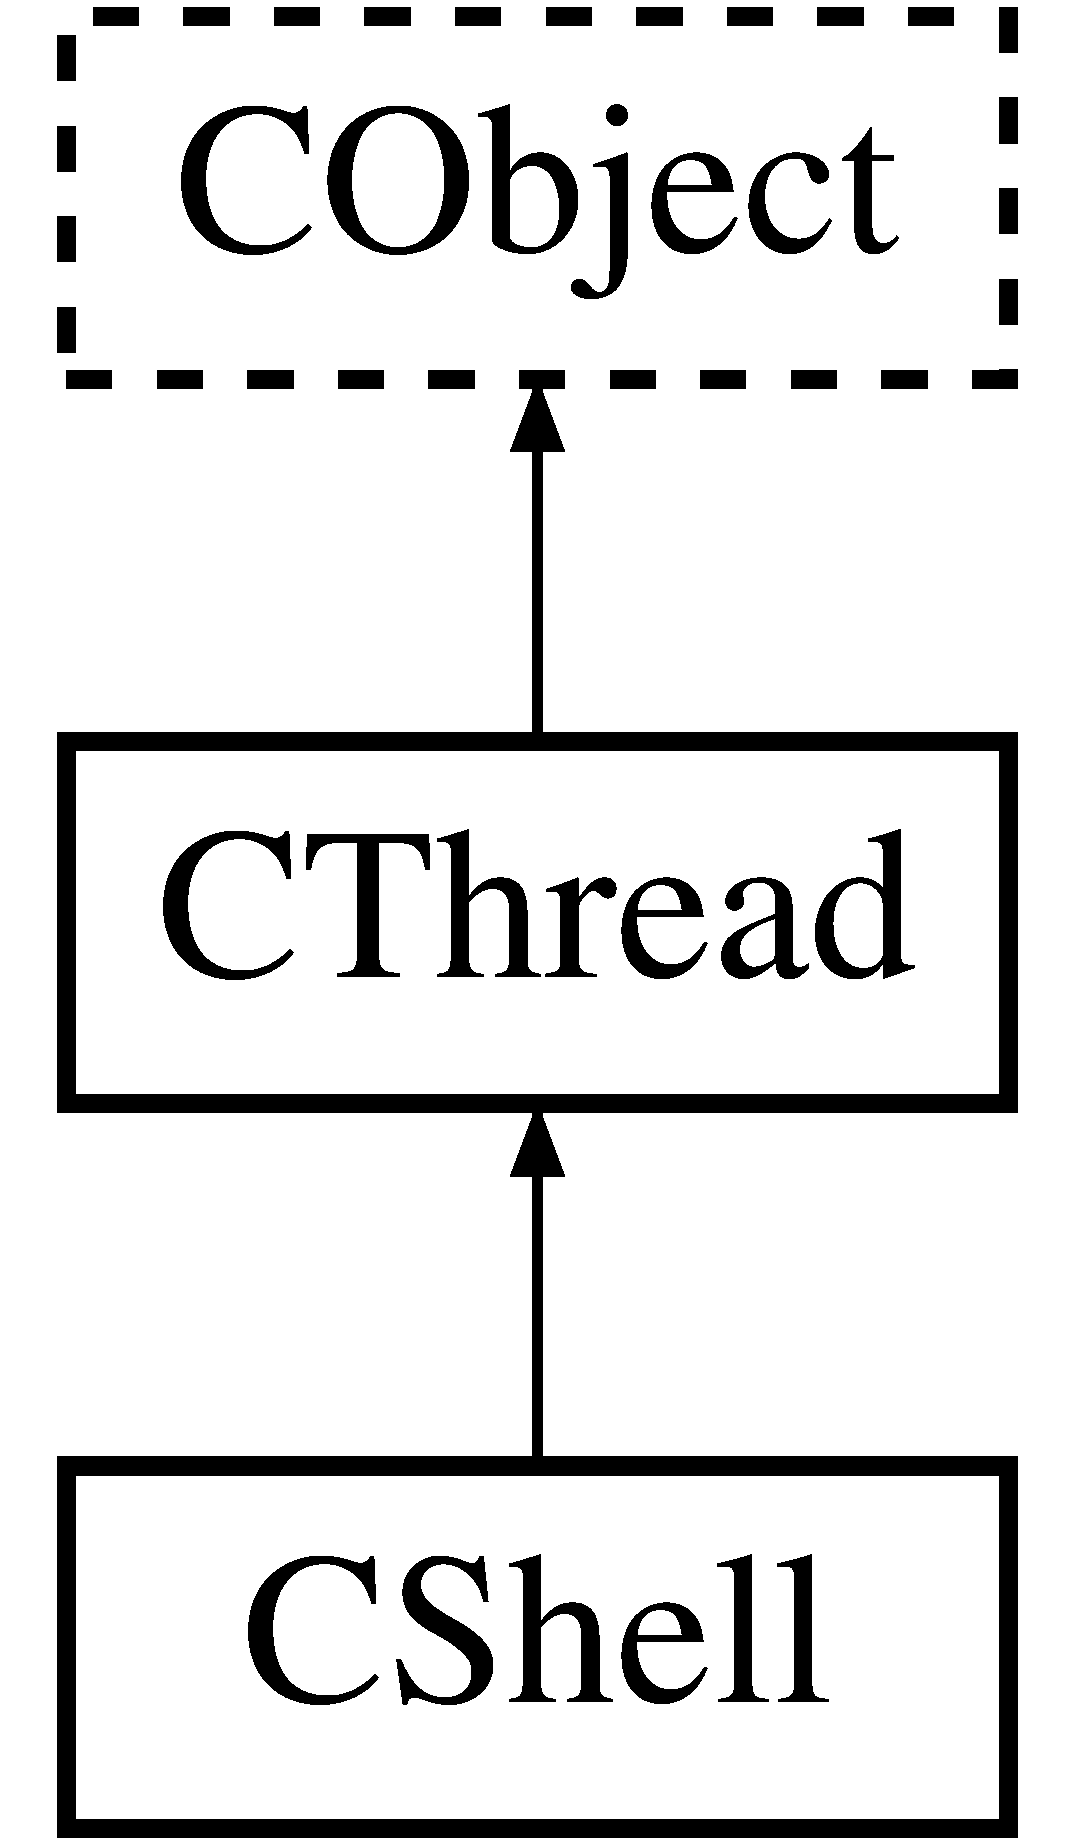
\includegraphics[height=3.000000cm]{de/dba/class_c_shell}
\end{center}
\end{figure}
\subsection*{Public Member Functions}
\begin{DoxyCompactItemize}
\item 
\hyperlink{class_c_shell_a66915a194065db1d82873d79ee6ec8c6}{C\-Shell} (\hyperlink{class_c_stream}{C\-Stream} \&s)
\item 
virtual bool \hyperlink{class_c_shell_a670f66f552494dfce94ee297ae0f659a}{start} ()
\item 
virtual void \hyperlink{class_c_shell_a16e1dae0dedda35c0be64d1c8f40e6b4}{on\-Query} (\hyperlink{class_c_string}{C\-String} \&str)
\item 
virtual void \hyperlink{class_c_shell_a34dfa6d370ce6fb517e1307d38a4982b}{show\-\_\-welcome} ()
\item 
virtual void \hyperlink{class_c_shell_a7adec131871fb1931300eb0f6b31b3f5}{show\-\_\-prompt} ()
\item 
virtual void \hyperlink{class_c_shell_ab499caffc2baf478802c3f89d606fc6c}{show\-\_\-menu} ()
\item 
virtual void \hyperlink{class_c_shell_ac9f0aa22624f3168256f6b6c851ec885}{show\-\_\-task} ()
\item 
virtual void \hyperlink{class_c_shell_a99cd1946dd501dd788accc421ffb883c}{show\-\_\-heap} ()
\item 
virtual void \hyperlink{class_c_shell_a4aed8c6a1e01a50595d9e8da8d1f88b2}{show\-\_\-version} ()
\item 
virtual void \hyperlink{class_c_shell_a8cb6ac07d2290e4d51c641af1d152b1f}{show\-\_\-clear} ()
\item 
bool \hyperlink{class_c_shell_ae0f6cb34ee627c44b1690d16d76d628f}{is\-Debug\-Mode} ()
\item 
int \hyperlink{class_c_shell_a7731a22b0b80a4facc431f6e07db2599}{dbg\-Wait\-Key} (uint32\-\_\-t t=M\-A\-X\-\_\-\-D\-E\-L\-A\-Y\-\_\-\-T\-I\-M\-E)
\item 
virtual void \hyperlink{class_c_shell_a1565a93fad9a1e35e05a597889ad130f}{run} ()
\item 
virtual void \hyperlink{class_c_shell_a74d294faaebd969b295366f4a861cf02}{on\-Debug} ()
\item 
virtual void \hyperlink{class_c_shell_a27a37bf5a22eaba1426655409decc188}{on\-Close} ()
\item 
virtual \hyperlink{class_c_shell_a342aa70c0ff0ba0f990942edfbc59bb6}{$\sim$\-C\-Shell} ()
\end{DoxyCompactItemize}
\subsection*{Public Attributes}
\begin{DoxyCompactItemize}
\item 
\hyperlink{class_console}{Console} \hyperlink{class_c_shell_ac555f42f70f60653dbd5e0c8ec9c4dcf}{m\-\_\-console}
\end{DoxyCompactItemize}
\subsection*{Protected Attributes}
\begin{DoxyCompactItemize}
\item 
\hyperlink{class_c_stream}{C\-Stream} $\ast$ \hyperlink{class_c_shell_ab0eaa18213db8965c68f978538050162}{m\-\_\-sock}
\item 
\hyperlink{class_c_string}{C\-String} \hyperlink{class_c_shell_aa5ef2d56e802b9925cf0ae7d36741bda}{cmd}
\item 
\hyperlink{class_c_semaphore}{C\-Semaphore} \hyperlink{class_c_shell_aa81828c40c17f38821ec395aaf38ee98}{m\-\_\-sem\-Input}
\item 
int \hyperlink{class_c_shell_ab2b6ca1616128e6a8a05c8c235c7b011}{m\-\_\-dbg\-Key}
\end{DoxyCompactItemize}
\subsection*{Additional Inherited Members}


\subsection{Constructor \& Destructor Documentation}
\hypertarget{class_c_shell_a66915a194065db1d82873d79ee6ec8c6}{\index{C\-Shell@{C\-Shell}!C\-Shell@{C\-Shell}}
\index{C\-Shell@{C\-Shell}!CShell@{C\-Shell}}
\subsubsection[{C\-Shell}]{\setlength{\rightskip}{0pt plus 5cm}C\-Shell\-::\-C\-Shell (
\begin{DoxyParamCaption}
\item[{{\bf C\-Stream} \&}]{s}
\end{DoxyParamCaption}
)}}\label{class_c_shell_a66915a194065db1d82873d79ee6ec8c6}
\hypertarget{class_c_shell_a342aa70c0ff0ba0f990942edfbc59bb6}{\index{C\-Shell@{C\-Shell}!$\sim$\-C\-Shell@{$\sim$\-C\-Shell}}
\index{$\sim$\-C\-Shell@{$\sim$\-C\-Shell}!CShell@{C\-Shell}}
\subsubsection[{$\sim$\-C\-Shell}]{\setlength{\rightskip}{0pt plus 5cm}virtual C\-Shell\-::$\sim$\-C\-Shell (
\begin{DoxyParamCaption}
{}
\end{DoxyParamCaption}
)\hspace{0.3cm}{\ttfamily [virtual]}}}\label{class_c_shell_a342aa70c0ff0ba0f990942edfbc59bb6}


\subsection{Member Function Documentation}
\hypertarget{class_c_shell_a670f66f552494dfce94ee297ae0f659a}{\index{C\-Shell@{C\-Shell}!start@{start}}
\index{start@{start}!CShell@{C\-Shell}}
\subsubsection[{start}]{\setlength{\rightskip}{0pt plus 5cm}virtual bool C\-Shell\-::start (
\begin{DoxyParamCaption}
{}
\end{DoxyParamCaption}
)\hspace{0.3cm}{\ttfamily [virtual]}}}\label{class_c_shell_a670f66f552494dfce94ee297ae0f659a}
Call the member function to start the thread. \begin{DoxyNote}{Note}
the \hyperlink{class_c_shell_a670f66f552494dfce94ee297ae0f659a}{start()} is an overload member function of \hyperlink{class_c_thread}{C\-Thread}. 
\end{DoxyNote}


Reimplemented from \hyperlink{class_c_thread_aacf955d1852e74da1f989251955ee6ec}{C\-Thread}.

\hypertarget{class_c_shell_a16e1dae0dedda35c0be64d1c8f40e6b4}{\index{C\-Shell@{C\-Shell}!on\-Query@{on\-Query}}
\index{on\-Query@{on\-Query}!CShell@{C\-Shell}}
\subsubsection[{on\-Query}]{\setlength{\rightskip}{0pt plus 5cm}virtual void C\-Shell\-::on\-Query (
\begin{DoxyParamCaption}
\item[{{\bf C\-String} \&}]{str}
\end{DoxyParamCaption}
)\hspace{0.3cm}{\ttfamily [virtual]}}}\label{class_c_shell_a16e1dae0dedda35c0be64d1c8f40e6b4}
\hypertarget{class_c_shell_a34dfa6d370ce6fb517e1307d38a4982b}{\index{C\-Shell@{C\-Shell}!show\-\_\-welcome@{show\-\_\-welcome}}
\index{show\-\_\-welcome@{show\-\_\-welcome}!CShell@{C\-Shell}}
\subsubsection[{show\-\_\-welcome}]{\setlength{\rightskip}{0pt plus 5cm}virtual void C\-Shell\-::show\-\_\-welcome (
\begin{DoxyParamCaption}
{}
\end{DoxyParamCaption}
)\hspace{0.3cm}{\ttfamily [virtual]}}}\label{class_c_shell_a34dfa6d370ce6fb517e1307d38a4982b}
\hypertarget{class_c_shell_a7adec131871fb1931300eb0f6b31b3f5}{\index{C\-Shell@{C\-Shell}!show\-\_\-prompt@{show\-\_\-prompt}}
\index{show\-\_\-prompt@{show\-\_\-prompt}!CShell@{C\-Shell}}
\subsubsection[{show\-\_\-prompt}]{\setlength{\rightskip}{0pt plus 5cm}virtual void C\-Shell\-::show\-\_\-prompt (
\begin{DoxyParamCaption}
{}
\end{DoxyParamCaption}
)\hspace{0.3cm}{\ttfamily [virtual]}}}\label{class_c_shell_a7adec131871fb1931300eb0f6b31b3f5}
\hypertarget{class_c_shell_ab499caffc2baf478802c3f89d606fc6c}{\index{C\-Shell@{C\-Shell}!show\-\_\-menu@{show\-\_\-menu}}
\index{show\-\_\-menu@{show\-\_\-menu}!CShell@{C\-Shell}}
\subsubsection[{show\-\_\-menu}]{\setlength{\rightskip}{0pt plus 5cm}virtual void C\-Shell\-::show\-\_\-menu (
\begin{DoxyParamCaption}
{}
\end{DoxyParamCaption}
)\hspace{0.3cm}{\ttfamily [virtual]}}}\label{class_c_shell_ab499caffc2baf478802c3f89d606fc6c}
\hypertarget{class_c_shell_ac9f0aa22624f3168256f6b6c851ec885}{\index{C\-Shell@{C\-Shell}!show\-\_\-task@{show\-\_\-task}}
\index{show\-\_\-task@{show\-\_\-task}!CShell@{C\-Shell}}
\subsubsection[{show\-\_\-task}]{\setlength{\rightskip}{0pt plus 5cm}virtual void C\-Shell\-::show\-\_\-task (
\begin{DoxyParamCaption}
{}
\end{DoxyParamCaption}
)\hspace{0.3cm}{\ttfamily [virtual]}}}\label{class_c_shell_ac9f0aa22624f3168256f6b6c851ec885}
\hypertarget{class_c_shell_a99cd1946dd501dd788accc421ffb883c}{\index{C\-Shell@{C\-Shell}!show\-\_\-heap@{show\-\_\-heap}}
\index{show\-\_\-heap@{show\-\_\-heap}!CShell@{C\-Shell}}
\subsubsection[{show\-\_\-heap}]{\setlength{\rightskip}{0pt plus 5cm}virtual void C\-Shell\-::show\-\_\-heap (
\begin{DoxyParamCaption}
{}
\end{DoxyParamCaption}
)\hspace{0.3cm}{\ttfamily [virtual]}}}\label{class_c_shell_a99cd1946dd501dd788accc421ffb883c}
\hypertarget{class_c_shell_a4aed8c6a1e01a50595d9e8da8d1f88b2}{\index{C\-Shell@{C\-Shell}!show\-\_\-version@{show\-\_\-version}}
\index{show\-\_\-version@{show\-\_\-version}!CShell@{C\-Shell}}
\subsubsection[{show\-\_\-version}]{\setlength{\rightskip}{0pt plus 5cm}virtual void C\-Shell\-::show\-\_\-version (
\begin{DoxyParamCaption}
{}
\end{DoxyParamCaption}
)\hspace{0.3cm}{\ttfamily [virtual]}}}\label{class_c_shell_a4aed8c6a1e01a50595d9e8da8d1f88b2}
\hypertarget{class_c_shell_a8cb6ac07d2290e4d51c641af1d152b1f}{\index{C\-Shell@{C\-Shell}!show\-\_\-clear@{show\-\_\-clear}}
\index{show\-\_\-clear@{show\-\_\-clear}!CShell@{C\-Shell}}
\subsubsection[{show\-\_\-clear}]{\setlength{\rightskip}{0pt plus 5cm}virtual void C\-Shell\-::show\-\_\-clear (
\begin{DoxyParamCaption}
{}
\end{DoxyParamCaption}
)\hspace{0.3cm}{\ttfamily [virtual]}}}\label{class_c_shell_a8cb6ac07d2290e4d51c641af1d152b1f}
\hypertarget{class_c_shell_ae0f6cb34ee627c44b1690d16d76d628f}{\index{C\-Shell@{C\-Shell}!is\-Debug\-Mode@{is\-Debug\-Mode}}
\index{is\-Debug\-Mode@{is\-Debug\-Mode}!CShell@{C\-Shell}}
\subsubsection[{is\-Debug\-Mode}]{\setlength{\rightskip}{0pt plus 5cm}bool C\-Shell\-::is\-Debug\-Mode (
\begin{DoxyParamCaption}
{}
\end{DoxyParamCaption}
)}}\label{class_c_shell_ae0f6cb34ee627c44b1690d16d76d628f}
\hypertarget{class_c_shell_a7731a22b0b80a4facc431f6e07db2599}{\index{C\-Shell@{C\-Shell}!dbg\-Wait\-Key@{dbg\-Wait\-Key}}
\index{dbg\-Wait\-Key@{dbg\-Wait\-Key}!CShell@{C\-Shell}}
\subsubsection[{dbg\-Wait\-Key}]{\setlength{\rightskip}{0pt plus 5cm}int C\-Shell\-::dbg\-Wait\-Key (
\begin{DoxyParamCaption}
\item[{uint32\-\_\-t}]{t = {\ttfamily MAX\-\_\-DELAY\-\_\-TIME}}
\end{DoxyParamCaption}
)}}\label{class_c_shell_a7731a22b0b80a4facc431f6e07db2599}
\hypertarget{class_c_shell_a1565a93fad9a1e35e05a597889ad130f}{\index{C\-Shell@{C\-Shell}!run@{run}}
\index{run@{run}!CShell@{C\-Shell}}
\subsubsection[{run}]{\setlength{\rightskip}{0pt plus 5cm}virtual void C\-Shell\-::run (
\begin{DoxyParamCaption}
{}
\end{DoxyParamCaption}
)\hspace{0.3cm}{\ttfamily [virtual]}}}\label{class_c_shell_a1565a93fad9a1e35e05a597889ad130f}
The run member function is the task main procedure, and callback by R\-T\-O\-S when task start.


\begin{DoxyCode}
Example:
        \textcolor{keyword}{class }CLedTask: \textcolor{keyword}{public} \hyperlink{class_c_thread}{CThread} \{
        \textcolor{keyword}{protected}:
            \textcolor{keyword}{virtual} \textcolor{keywordtype}{void} \hyperlink{class_c_shell_a1565a93fad9a1e35e05a597889ad130f}{run}() \{
                \hyperlink{class_c_pin}{CPin} led(LED2);
                \textcolor{keywordflow}{while}(1) \{
                    led = !led;
                    sleep(200);
                \}
            \}
        \};

        \textcolor{keywordtype}{int} main() \{
            ...
            CLedTask ledTask;
            ledTask.start(\textcolor{stringliteral}{"led"});   \textcolor{comment}{// default stack=128, default priority=low}
            ...
        \}
\end{DoxyCode}
 \begin{DoxyRemark}{Remarks}
The \hyperlink{class_c_shell_a1565a93fad9a1e35e05a597889ad130f}{run()} is a pure virtual function, must reimplement by inheritor. 
\end{DoxyRemark}
\begin{DoxyNote}{Note}
if end the \hyperlink{class_c_shell_a1565a93fad9a1e35e05a597889ad130f}{run()} member function, the \hyperlink{class_c_thread}{C\-Thread} object will be deleted and collected. 
\end{DoxyNote}


Reimplemented from \hyperlink{class_c_thread_a071c3d3b3c19a7bd6a01aca073a9b4d7}{C\-Thread}.

\hypertarget{class_c_shell_a74d294faaebd969b295366f4a861cf02}{\index{C\-Shell@{C\-Shell}!on\-Debug@{on\-Debug}}
\index{on\-Debug@{on\-Debug}!CShell@{C\-Shell}}
\subsubsection[{on\-Debug}]{\setlength{\rightskip}{0pt plus 5cm}virtual void C\-Shell\-::on\-Debug (
\begin{DoxyParamCaption}
{}
\end{DoxyParamCaption}
)\hspace{0.3cm}{\ttfamily [virtual]}}}\label{class_c_shell_a74d294faaebd969b295366f4a861cf02}
\hypertarget{class_c_shell_a27a37bf5a22eaba1426655409decc188}{\index{C\-Shell@{C\-Shell}!on\-Close@{on\-Close}}
\index{on\-Close@{on\-Close}!CShell@{C\-Shell}}
\subsubsection[{on\-Close}]{\setlength{\rightskip}{0pt plus 5cm}virtual void C\-Shell\-::on\-Close (
\begin{DoxyParamCaption}
{}
\end{DoxyParamCaption}
)\hspace{0.3cm}{\ttfamily [inline]}, {\ttfamily [virtual]}}}\label{class_c_shell_a27a37bf5a22eaba1426655409decc188}


\subsection{Member Data Documentation}
\hypertarget{class_c_shell_ac555f42f70f60653dbd5e0c8ec9c4dcf}{\index{C\-Shell@{C\-Shell}!m\-\_\-console@{m\-\_\-console}}
\index{m\-\_\-console@{m\-\_\-console}!CShell@{C\-Shell}}
\subsubsection[{m\-\_\-console}]{\setlength{\rightskip}{0pt plus 5cm}{\bf Console} C\-Shell\-::m\-\_\-console}}\label{class_c_shell_ac555f42f70f60653dbd5e0c8ec9c4dcf}
\hypertarget{class_c_shell_ab0eaa18213db8965c68f978538050162}{\index{C\-Shell@{C\-Shell}!m\-\_\-sock@{m\-\_\-sock}}
\index{m\-\_\-sock@{m\-\_\-sock}!CShell@{C\-Shell}}
\subsubsection[{m\-\_\-sock}]{\setlength{\rightskip}{0pt plus 5cm}{\bf C\-Stream}$\ast$ C\-Shell\-::m\-\_\-sock\hspace{0.3cm}{\ttfamily [protected]}}}\label{class_c_shell_ab0eaa18213db8965c68f978538050162}
\hypertarget{class_c_shell_aa5ef2d56e802b9925cf0ae7d36741bda}{\index{C\-Shell@{C\-Shell}!cmd@{cmd}}
\index{cmd@{cmd}!CShell@{C\-Shell}}
\subsubsection[{cmd}]{\setlength{\rightskip}{0pt plus 5cm}{\bf C\-String} C\-Shell\-::cmd\hspace{0.3cm}{\ttfamily [protected]}}}\label{class_c_shell_aa5ef2d56e802b9925cf0ae7d36741bda}
\hypertarget{class_c_shell_aa81828c40c17f38821ec395aaf38ee98}{\index{C\-Shell@{C\-Shell}!m\-\_\-sem\-Input@{m\-\_\-sem\-Input}}
\index{m\-\_\-sem\-Input@{m\-\_\-sem\-Input}!CShell@{C\-Shell}}
\subsubsection[{m\-\_\-sem\-Input}]{\setlength{\rightskip}{0pt plus 5cm}{\bf C\-Semaphore} C\-Shell\-::m\-\_\-sem\-Input\hspace{0.3cm}{\ttfamily [protected]}}}\label{class_c_shell_aa81828c40c17f38821ec395aaf38ee98}
\hypertarget{class_c_shell_ab2b6ca1616128e6a8a05c8c235c7b011}{\index{C\-Shell@{C\-Shell}!m\-\_\-dbg\-Key@{m\-\_\-dbg\-Key}}
\index{m\-\_\-dbg\-Key@{m\-\_\-dbg\-Key}!CShell@{C\-Shell}}
\subsubsection[{m\-\_\-dbg\-Key}]{\setlength{\rightskip}{0pt plus 5cm}int C\-Shell\-::m\-\_\-dbg\-Key\hspace{0.3cm}{\ttfamily [protected]}}}\label{class_c_shell_ab2b6ca1616128e6a8a05c8c235c7b011}


The documentation for this class was generated from the following file\-:\begin{DoxyCompactItemize}
\item 
shell.\-h\end{DoxyCompactItemize}

\hypertarget{class_c_small_printf}{\section{C\-Small\-Printf Class Reference}
\label{class_c_small_printf}\index{C\-Small\-Printf@{C\-Small\-Printf}}
}


{\ttfamily \#include $<$smallprintf.\-h$>$}

Inheritance diagram for C\-Small\-Printf\-:\begin{figure}[H]
\begin{center}
\leavevmode
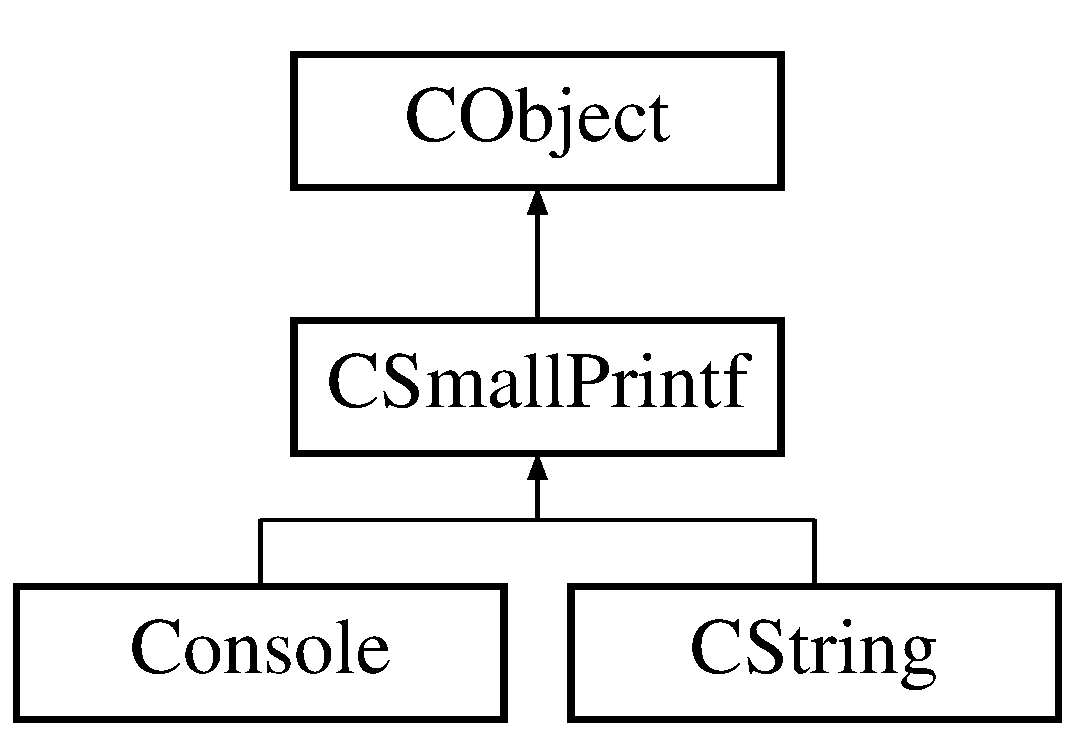
\includegraphics[height=3.000000cm]{de/db4/class_c_small_printf}
\end{center}
\end{figure}
\subsection*{Public Member Functions}
\begin{DoxyCompactItemize}
\item 
\hyperlink{class_c_small_printf_a4d3c439b597dde5df178d189a5eb4024}{C\-Small\-Printf} ()
\item 
int \hyperlink{class_c_small_printf_a6213c847987bc1cf18b980619ca49db7}{printf} (L\-P\-C\-T\-S\-T\-R format,...)
\item 
int \hyperlink{class_c_small_printf_a651d3546ffbbe986fbbbf4bb1043bb7b}{printf} (L\-P\-C\-T\-S\-T\-R format, va\-\_\-list args)
\item 
int \hyperlink{class_c_small_printf_a158dc1f45a1f19c8edd63e22544c30cc}{putv} (int val)
\item 
int \hyperlink{class_c_small_printf_a4396d279d38afdf4fd71514760b6ace3}{putv} (unsigned val)
\item 
int \hyperlink{class_c_small_printf_a9158226f537c34067bf2e6a7c25d3f8b}{putv} (double val)
\end{DoxyCompactItemize}


\subsection{Constructor \& Destructor Documentation}
\hypertarget{class_c_small_printf_a4d3c439b597dde5df178d189a5eb4024}{\index{C\-Small\-Printf@{C\-Small\-Printf}!C\-Small\-Printf@{C\-Small\-Printf}}
\index{C\-Small\-Printf@{C\-Small\-Printf}!CSmallPrintf@{C\-Small\-Printf}}
\subsubsection[{C\-Small\-Printf}]{\setlength{\rightskip}{0pt plus 5cm}C\-Small\-Printf\-::\-C\-Small\-Printf (
\begin{DoxyParamCaption}
{}
\end{DoxyParamCaption}
)}}\label{class_c_small_printf_a4d3c439b597dde5df178d189a5eb4024}


\subsection{Member Function Documentation}
\hypertarget{class_c_small_printf_a6213c847987bc1cf18b980619ca49db7}{\index{C\-Small\-Printf@{C\-Small\-Printf}!printf@{printf}}
\index{printf@{printf}!CSmallPrintf@{C\-Small\-Printf}}
\subsubsection[{printf}]{\setlength{\rightskip}{0pt plus 5cm}int C\-Small\-Printf\-::printf (
\begin{DoxyParamCaption}
\item[{L\-P\-C\-T\-S\-T\-R}]{format, }
\item[{}]{...}
\end{DoxyParamCaption}
)}}\label{class_c_small_printf_a6213c847987bc1cf18b980619ca49db7}
\hypertarget{class_c_small_printf_a651d3546ffbbe986fbbbf4bb1043bb7b}{\index{C\-Small\-Printf@{C\-Small\-Printf}!printf@{printf}}
\index{printf@{printf}!CSmallPrintf@{C\-Small\-Printf}}
\subsubsection[{printf}]{\setlength{\rightskip}{0pt plus 5cm}int C\-Small\-Printf\-::printf (
\begin{DoxyParamCaption}
\item[{L\-P\-C\-T\-S\-T\-R}]{format, }
\item[{va\-\_\-list}]{args}
\end{DoxyParamCaption}
)}}\label{class_c_small_printf_a651d3546ffbbe986fbbbf4bb1043bb7b}
\hypertarget{class_c_small_printf_a158dc1f45a1f19c8edd63e22544c30cc}{\index{C\-Small\-Printf@{C\-Small\-Printf}!putv@{putv}}
\index{putv@{putv}!CSmallPrintf@{C\-Small\-Printf}}
\subsubsection[{putv}]{\setlength{\rightskip}{0pt plus 5cm}int C\-Small\-Printf\-::putv (
\begin{DoxyParamCaption}
\item[{int}]{val}
\end{DoxyParamCaption}
)}}\label{class_c_small_printf_a158dc1f45a1f19c8edd63e22544c30cc}
\hypertarget{class_c_small_printf_a4396d279d38afdf4fd71514760b6ace3}{\index{C\-Small\-Printf@{C\-Small\-Printf}!putv@{putv}}
\index{putv@{putv}!CSmallPrintf@{C\-Small\-Printf}}
\subsubsection[{putv}]{\setlength{\rightskip}{0pt plus 5cm}int C\-Small\-Printf\-::putv (
\begin{DoxyParamCaption}
\item[{unsigned}]{val}
\end{DoxyParamCaption}
)}}\label{class_c_small_printf_a4396d279d38afdf4fd71514760b6ace3}
\hypertarget{class_c_small_printf_a9158226f537c34067bf2e6a7c25d3f8b}{\index{C\-Small\-Printf@{C\-Small\-Printf}!putv@{putv}}
\index{putv@{putv}!CSmallPrintf@{C\-Small\-Printf}}
\subsubsection[{putv}]{\setlength{\rightskip}{0pt plus 5cm}int C\-Small\-Printf\-::putv (
\begin{DoxyParamCaption}
\item[{double}]{val}
\end{DoxyParamCaption}
)}}\label{class_c_small_printf_a9158226f537c34067bf2e6a7c25d3f8b}


The documentation for this class was generated from the following file\-:\begin{DoxyCompactItemize}
\item 
smallprintf.\-h\end{DoxyCompactItemize}

\hypertarget{class_c_s_p_i}{\section{C\-S\-P\-I Class Reference}
\label{class_c_s_p_i}\index{C\-S\-P\-I@{C\-S\-P\-I}}
}


{\ttfamily \#include \char`\"{}class/spi.\-h\char`\"{}}

Inheritance diagram for C\-S\-P\-I\-:\begin{figure}[H]
\begin{center}
\leavevmode
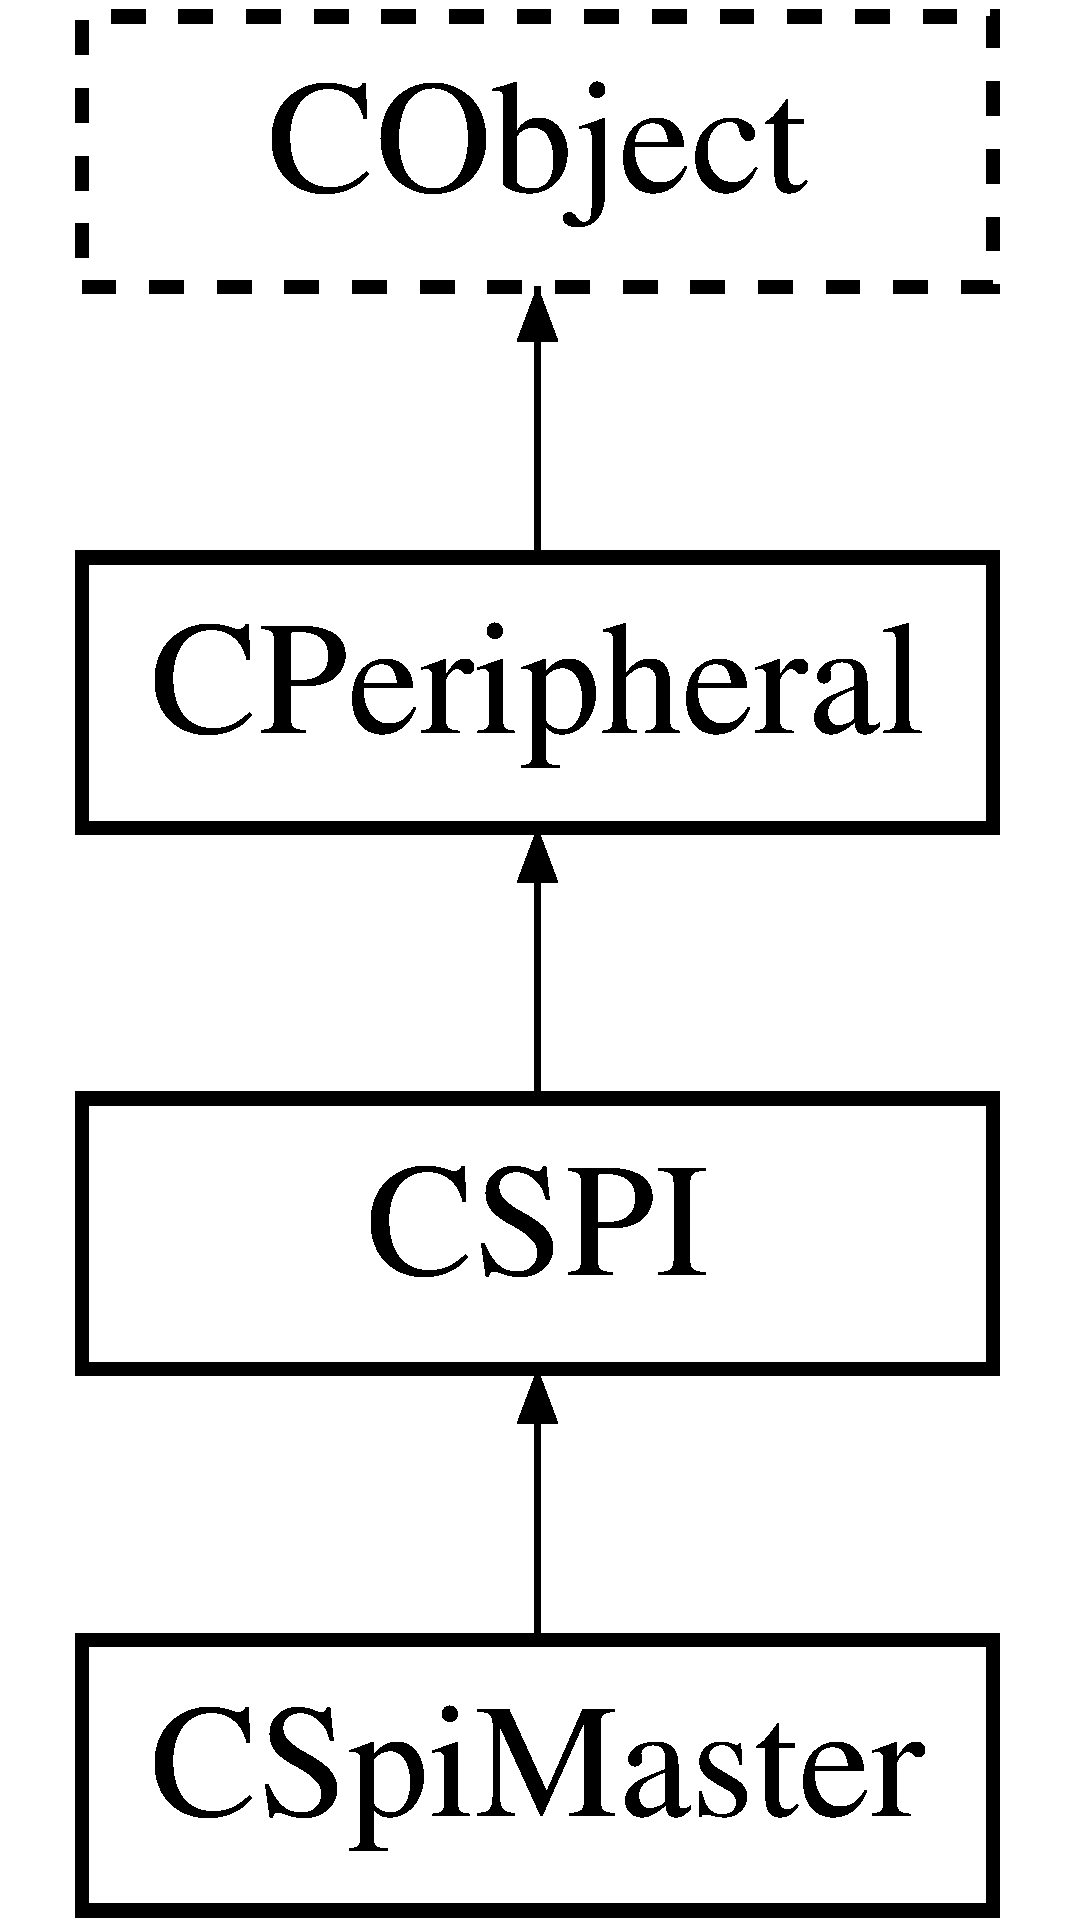
\includegraphics[height=4.000000cm]{d2/d3f/class_c_s_p_i}
\end{center}
\end{figure}
\subsection*{Public Member Functions}
\begin{DoxyCompactItemize}
\item 
\hyperlink{class_c_s_p_i_a45ebc1852b74f5f0ccfbb97b302cf5e9}{C\-S\-P\-I} (\hyperlink{group___enumerations_ga1adbe6bf70e3880dc6b9f86e58bb7f98}{S\-P\-I\-\_\-\-P\-O\-R\-T\-\_\-\-T} port=\hyperlink{group___enumerations_gga1adbe6bf70e3880dc6b9f86e58bb7f98a7add1e0588a075d9385b10fcbb2010f4}{S\-P\-I0}, bool pullup=true)
\item 
virtual \hyperlink{class_c_s_p_i_ade8c01d1d751682ededa1cb27ab85409}{$\sim$\-C\-S\-P\-I} ()
\item 
void \hyperlink{class_c_s_p_i_accc9a5c831ee85e95f0bb5567de5f529}{format} (S\-P\-I\-\_\-\-D\-A\-T\-A\-B\-I\-T\-\_\-\-T bits, S\-P\-I\-\_\-\-M\-O\-D\-E\-\_\-\-T mode=S\-P\-I\-\_\-\-M\-O\-D\-E\-\_\-0)
\item 
void \hyperlink{class_c_s_p_i_aa7a160dad74689b9afb720c78d63558f}{bit\-Order} (S\-P\-I\-\_\-\-B\-I\-T\-\_\-\-O\-R\-D\-E\-R\-\_\-\-T value)
\item 
bool \hyperlink{class_c_s_p_i_ad8143fa5be48bc62762fda52b86d630a}{frequency} (uint32\-\_\-t hz)
\item 
virtual void \hyperlink{class_c_s_p_i_a7dc9ce9f0b38a59f7332e6f4f39864e8}{enable} (S\-P\-I\-\_\-\-R\-O\-L\-E\-\_\-\-T role=S\-P\-I\-\_\-\-M\-A\-S\-T\-E\-R)
\item 
virtual void \hyperlink{class_c_s_p_i_a5009ac7cc08bcf2b1d1be19b320424e6}{disable} ()
\item 
bool \hyperlink{class_c_s_p_i_ab237c0acc917287a8f7cdca7e91e87c6}{is\-Slave} ()
\item 
void \hyperlink{class_c_s_p_i_a98fb4712f52c9977d4973430f5f505b8}{begin} (S\-P\-I\-\_\-\-R\-O\-L\-E\-\_\-\-T role=S\-P\-I\-\_\-\-M\-A\-S\-T\-E\-R)
\item 
void \hyperlink{class_c_s_p_i_a9a8f9843e54bf4f11dd871cf798fe337}{end} ()
\item 
virtual int \hyperlink{class_c_s_p_i_a5215a320db4cb5f2792ea18f8d6e0671}{readwrite} (void $\ast$txbuf, void $\ast$rxbuf, uint32\-\_\-t length)
\item 
int \hyperlink{class_c_s_p_i_a0cdfe6a4d42e835cf7b67ba99ae115ca}{readwrite} (uint8\-\_\-t tx, uint8\-\_\-t \&rx)
\item 
uint8\-\_\-t \hyperlink{class_c_s_p_i_acf2e1695f717fa88620e4bddd7871ea3}{readwrite} (uint8\-\_\-t tx)
\item 
uint8\-\_\-t \hyperlink{class_c_s_p_i_a2b91318925ae9de3f295abd2418285c4}{write} (uint8\-\_\-t tx)
\item 
void \hyperlink{class_c_s_p_i_a24ca202a0494b84a92ff56d10725ce40}{operator$>$$>$} (uint8\-\_\-t \&val)
\item 
void \hyperlink{class_c_s_p_i_a3ce438bee4e3c087e44b3cf2b1690ecd}{operator$<$$<$} (uint8\-\_\-t val)
\item 
void \hyperlink{class_c_s_p_i_ac53ab106be8d0f369b349f82b3db6813}{operator$>$$>$} (uint16\-\_\-t \&val)
\item 
void \hyperlink{class_c_s_p_i_a272f5e518d21194dbc996f5f5475ae02}{operator$<$$<$} (uint16\-\_\-t val)
\item 
void \hyperlink{class_c_s_p_i_aaf1a92290aaee5a93f8fc2db9ce4a512}{operator$>$$>$} (uint32\-\_\-t \&val)
\item 
void \hyperlink{class_c_s_p_i_a4d0cd48d0bba271fd72df43d7528e2a0}{operator$<$$<$} (uint32\-\_\-t val)
\end{DoxyCompactItemize}
\subsection*{Protected Attributes}
\begin{DoxyCompactItemize}
\item 
\hyperlink{group___enumerations_ga1adbe6bf70e3880dc6b9f86e58bb7f98}{S\-P\-I\-\_\-\-P\-O\-R\-T\-\_\-\-T} \hyperlink{class_c_s_p_i_a44669f2150e9312a3bd022c000574f81}{m\-\_\-port}
\item 
uint32\-\_\-t \hyperlink{class_c_s_p_i_a63f794ebd52c8a7402c1327cd84986ed}{m\-\_\-n\-Flag}
\end{DoxyCompactItemize}


\subsection{Detailed Description}
\hyperlink{class_c_s_p_i}{C\-S\-P\-I} class provides the Serial Peripheral Interface. 

\subsection{Constructor \& Destructor Documentation}
\hypertarget{class_c_s_p_i_a45ebc1852b74f5f0ccfbb97b302cf5e9}{\index{C\-S\-P\-I@{C\-S\-P\-I}!C\-S\-P\-I@{C\-S\-P\-I}}
\index{C\-S\-P\-I@{C\-S\-P\-I}!CSPI@{C\-S\-P\-I}}
\subsubsection[{C\-S\-P\-I}]{\setlength{\rightskip}{0pt plus 5cm}C\-S\-P\-I\-::\-C\-S\-P\-I (
\begin{DoxyParamCaption}
\item[{{\bf S\-P\-I\-\_\-\-P\-O\-R\-T\-\_\-\-T}}]{port = {\ttfamily {\bf S\-P\-I0}}, }
\item[{bool}]{pullup = {\ttfamily true}}
\end{DoxyParamCaption}
)}}\label{class_c_s_p_i_a45ebc1852b74f5f0ccfbb97b302cf5e9}
\hypertarget{class_c_s_p_i_ade8c01d1d751682ededa1cb27ab85409}{\index{C\-S\-P\-I@{C\-S\-P\-I}!$\sim$\-C\-S\-P\-I@{$\sim$\-C\-S\-P\-I}}
\index{$\sim$\-C\-S\-P\-I@{$\sim$\-C\-S\-P\-I}!CSPI@{C\-S\-P\-I}}
\subsubsection[{$\sim$\-C\-S\-P\-I}]{\setlength{\rightskip}{0pt plus 5cm}virtual C\-S\-P\-I\-::$\sim$\-C\-S\-P\-I (
\begin{DoxyParamCaption}
{}
\end{DoxyParamCaption}
)\hspace{0.3cm}{\ttfamily [virtual]}}}\label{class_c_s_p_i_ade8c01d1d751682ededa1cb27ab85409}


\subsection{Member Function Documentation}
\hypertarget{class_c_s_p_i_accc9a5c831ee85e95f0bb5567de5f529}{\index{C\-S\-P\-I@{C\-S\-P\-I}!format@{format}}
\index{format@{format}!CSPI@{C\-S\-P\-I}}
\subsubsection[{format}]{\setlength{\rightskip}{0pt plus 5cm}void C\-S\-P\-I\-::format (
\begin{DoxyParamCaption}
\item[{S\-P\-I\-\_\-\-D\-A\-T\-A\-B\-I\-T\-\_\-\-T}]{bits, }
\item[{S\-P\-I\-\_\-\-M\-O\-D\-E\-\_\-\-T}]{mode = {\ttfamily SPI\-\_\-MODE\-\_\-0}}
\end{DoxyParamCaption}
)}}\label{class_c_s_p_i_accc9a5c831ee85e95f0bb5567de5f529}
\hypertarget{class_c_s_p_i_aa7a160dad74689b9afb720c78d63558f}{\index{C\-S\-P\-I@{C\-S\-P\-I}!bit\-Order@{bit\-Order}}
\index{bit\-Order@{bit\-Order}!CSPI@{C\-S\-P\-I}}
\subsubsection[{bit\-Order}]{\setlength{\rightskip}{0pt plus 5cm}void C\-S\-P\-I\-::bit\-Order (
\begin{DoxyParamCaption}
\item[{S\-P\-I\-\_\-\-B\-I\-T\-\_\-\-O\-R\-D\-E\-R\-\_\-\-T}]{value}
\end{DoxyParamCaption}
)}}\label{class_c_s_p_i_aa7a160dad74689b9afb720c78d63558f}
\hypertarget{class_c_s_p_i_ad8143fa5be48bc62762fda52b86d630a}{\index{C\-S\-P\-I@{C\-S\-P\-I}!frequency@{frequency}}
\index{frequency@{frequency}!CSPI@{C\-S\-P\-I}}
\subsubsection[{frequency}]{\setlength{\rightskip}{0pt plus 5cm}bool C\-S\-P\-I\-::frequency (
\begin{DoxyParamCaption}
\item[{uint32\-\_\-t}]{hz}
\end{DoxyParamCaption}
)}}\label{class_c_s_p_i_ad8143fa5be48bc62762fda52b86d630a}
\hypertarget{class_c_s_p_i_a7dc9ce9f0b38a59f7332e6f4f39864e8}{\index{C\-S\-P\-I@{C\-S\-P\-I}!enable@{enable}}
\index{enable@{enable}!CSPI@{C\-S\-P\-I}}
\subsubsection[{enable}]{\setlength{\rightskip}{0pt plus 5cm}virtual void C\-S\-P\-I\-::enable (
\begin{DoxyParamCaption}
\item[{S\-P\-I\-\_\-\-R\-O\-L\-E\-\_\-\-T}]{role = {\ttfamily SPI\-\_\-MASTER}}
\end{DoxyParamCaption}
)\hspace{0.3cm}{\ttfamily [virtual]}}}\label{class_c_s_p_i_a7dc9ce9f0b38a59f7332e6f4f39864e8}
\hypertarget{class_c_s_p_i_a5009ac7cc08bcf2b1d1be19b320424e6}{\index{C\-S\-P\-I@{C\-S\-P\-I}!disable@{disable}}
\index{disable@{disable}!CSPI@{C\-S\-P\-I}}
\subsubsection[{disable}]{\setlength{\rightskip}{0pt plus 5cm}virtual void C\-S\-P\-I\-::disable (
\begin{DoxyParamCaption}
{}
\end{DoxyParamCaption}
)\hspace{0.3cm}{\ttfamily [virtual]}}}\label{class_c_s_p_i_a5009ac7cc08bcf2b1d1be19b320424e6}
\hypertarget{class_c_s_p_i_ab237c0acc917287a8f7cdca7e91e87c6}{\index{C\-S\-P\-I@{C\-S\-P\-I}!is\-Slave@{is\-Slave}}
\index{is\-Slave@{is\-Slave}!CSPI@{C\-S\-P\-I}}
\subsubsection[{is\-Slave}]{\setlength{\rightskip}{0pt plus 5cm}bool C\-S\-P\-I\-::is\-Slave (
\begin{DoxyParamCaption}
{}
\end{DoxyParamCaption}
)}}\label{class_c_s_p_i_ab237c0acc917287a8f7cdca7e91e87c6}
\hypertarget{class_c_s_p_i_a98fb4712f52c9977d4973430f5f505b8}{\index{C\-S\-P\-I@{C\-S\-P\-I}!begin@{begin}}
\index{begin@{begin}!CSPI@{C\-S\-P\-I}}
\subsubsection[{begin}]{\setlength{\rightskip}{0pt plus 5cm}void C\-S\-P\-I\-::begin (
\begin{DoxyParamCaption}
\item[{S\-P\-I\-\_\-\-R\-O\-L\-E\-\_\-\-T}]{role = {\ttfamily SPI\-\_\-MASTER}}
\end{DoxyParamCaption}
)\hspace{0.3cm}{\ttfamily [inline]}}}\label{class_c_s_p_i_a98fb4712f52c9977d4973430f5f505b8}
\hypertarget{class_c_s_p_i_a9a8f9843e54bf4f11dd871cf798fe337}{\index{C\-S\-P\-I@{C\-S\-P\-I}!end@{end}}
\index{end@{end}!CSPI@{C\-S\-P\-I}}
\subsubsection[{end}]{\setlength{\rightskip}{0pt plus 5cm}void C\-S\-P\-I\-::end (
\begin{DoxyParamCaption}
{}
\end{DoxyParamCaption}
)\hspace{0.3cm}{\ttfamily [inline]}}}\label{class_c_s_p_i_a9a8f9843e54bf4f11dd871cf798fe337}
\hypertarget{class_c_s_p_i_a5215a320db4cb5f2792ea18f8d6e0671}{\index{C\-S\-P\-I@{C\-S\-P\-I}!readwrite@{readwrite}}
\index{readwrite@{readwrite}!CSPI@{C\-S\-P\-I}}
\subsubsection[{readwrite}]{\setlength{\rightskip}{0pt plus 5cm}virtual int C\-S\-P\-I\-::readwrite (
\begin{DoxyParamCaption}
\item[{void $\ast$}]{txbuf, }
\item[{void $\ast$}]{rxbuf, }
\item[{uint32\-\_\-t}]{length}
\end{DoxyParamCaption}
)\hspace{0.3cm}{\ttfamily [virtual]}}}\label{class_c_s_p_i_a5215a320db4cb5f2792ea18f8d6e0671}


Reimplemented in \hyperlink{class_c_spi_master_a13d1514765c41561d16dd46eefb9926e}{C\-Spi\-Master}.

\hypertarget{class_c_s_p_i_a0cdfe6a4d42e835cf7b67ba99ae115ca}{\index{C\-S\-P\-I@{C\-S\-P\-I}!readwrite@{readwrite}}
\index{readwrite@{readwrite}!CSPI@{C\-S\-P\-I}}
\subsubsection[{readwrite}]{\setlength{\rightskip}{0pt plus 5cm}int C\-S\-P\-I\-::readwrite (
\begin{DoxyParamCaption}
\item[{uint8\-\_\-t}]{tx, }
\item[{uint8\-\_\-t \&}]{rx}
\end{DoxyParamCaption}
)\hspace{0.3cm}{\ttfamily [inline]}}}\label{class_c_s_p_i_a0cdfe6a4d42e835cf7b67ba99ae115ca}
\hypertarget{class_c_s_p_i_acf2e1695f717fa88620e4bddd7871ea3}{\index{C\-S\-P\-I@{C\-S\-P\-I}!readwrite@{readwrite}}
\index{readwrite@{readwrite}!CSPI@{C\-S\-P\-I}}
\subsubsection[{readwrite}]{\setlength{\rightskip}{0pt plus 5cm}uint8\-\_\-t C\-S\-P\-I\-::readwrite (
\begin{DoxyParamCaption}
\item[{uint8\-\_\-t}]{tx}
\end{DoxyParamCaption}
)\hspace{0.3cm}{\ttfamily [inline]}}}\label{class_c_s_p_i_acf2e1695f717fa88620e4bddd7871ea3}
\hypertarget{class_c_s_p_i_a2b91318925ae9de3f295abd2418285c4}{\index{C\-S\-P\-I@{C\-S\-P\-I}!write@{write}}
\index{write@{write}!CSPI@{C\-S\-P\-I}}
\subsubsection[{write}]{\setlength{\rightskip}{0pt plus 5cm}uint8\-\_\-t C\-S\-P\-I\-::write (
\begin{DoxyParamCaption}
\item[{uint8\-\_\-t}]{tx}
\end{DoxyParamCaption}
)\hspace{0.3cm}{\ttfamily [inline]}}}\label{class_c_s_p_i_a2b91318925ae9de3f295abd2418285c4}
\hypertarget{class_c_s_p_i_a24ca202a0494b84a92ff56d10725ce40}{\index{C\-S\-P\-I@{C\-S\-P\-I}!operator$>$$>$@{operator$>$$>$}}
\index{operator$>$$>$@{operator$>$$>$}!CSPI@{C\-S\-P\-I}}
\subsubsection[{operator$>$$>$}]{\setlength{\rightskip}{0pt plus 5cm}void C\-S\-P\-I\-::operator$>$$>$ (
\begin{DoxyParamCaption}
\item[{uint8\-\_\-t \&}]{val}
\end{DoxyParamCaption}
)\hspace{0.3cm}{\ttfamily [inline]}}}\label{class_c_s_p_i_a24ca202a0494b84a92ff56d10725ce40}
\hypertarget{class_c_s_p_i_a3ce438bee4e3c087e44b3cf2b1690ecd}{\index{C\-S\-P\-I@{C\-S\-P\-I}!operator$<$$<$@{operator$<$$<$}}
\index{operator$<$$<$@{operator$<$$<$}!CSPI@{C\-S\-P\-I}}
\subsubsection[{operator$<$$<$}]{\setlength{\rightskip}{0pt plus 5cm}void C\-S\-P\-I\-::operator$<$$<$ (
\begin{DoxyParamCaption}
\item[{uint8\-\_\-t}]{val}
\end{DoxyParamCaption}
)\hspace{0.3cm}{\ttfamily [inline]}}}\label{class_c_s_p_i_a3ce438bee4e3c087e44b3cf2b1690ecd}
\hypertarget{class_c_s_p_i_ac53ab106be8d0f369b349f82b3db6813}{\index{C\-S\-P\-I@{C\-S\-P\-I}!operator$>$$>$@{operator$>$$>$}}
\index{operator$>$$>$@{operator$>$$>$}!CSPI@{C\-S\-P\-I}}
\subsubsection[{operator$>$$>$}]{\setlength{\rightskip}{0pt plus 5cm}void C\-S\-P\-I\-::operator$>$$>$ (
\begin{DoxyParamCaption}
\item[{uint16\-\_\-t \&}]{val}
\end{DoxyParamCaption}
)\hspace{0.3cm}{\ttfamily [inline]}}}\label{class_c_s_p_i_ac53ab106be8d0f369b349f82b3db6813}
\hypertarget{class_c_s_p_i_a272f5e518d21194dbc996f5f5475ae02}{\index{C\-S\-P\-I@{C\-S\-P\-I}!operator$<$$<$@{operator$<$$<$}}
\index{operator$<$$<$@{operator$<$$<$}!CSPI@{C\-S\-P\-I}}
\subsubsection[{operator$<$$<$}]{\setlength{\rightskip}{0pt plus 5cm}void C\-S\-P\-I\-::operator$<$$<$ (
\begin{DoxyParamCaption}
\item[{uint16\-\_\-t}]{val}
\end{DoxyParamCaption}
)\hspace{0.3cm}{\ttfamily [inline]}}}\label{class_c_s_p_i_a272f5e518d21194dbc996f5f5475ae02}
\hypertarget{class_c_s_p_i_aaf1a92290aaee5a93f8fc2db9ce4a512}{\index{C\-S\-P\-I@{C\-S\-P\-I}!operator$>$$>$@{operator$>$$>$}}
\index{operator$>$$>$@{operator$>$$>$}!CSPI@{C\-S\-P\-I}}
\subsubsection[{operator$>$$>$}]{\setlength{\rightskip}{0pt plus 5cm}void C\-S\-P\-I\-::operator$>$$>$ (
\begin{DoxyParamCaption}
\item[{uint32\-\_\-t \&}]{val}
\end{DoxyParamCaption}
)\hspace{0.3cm}{\ttfamily [inline]}}}\label{class_c_s_p_i_aaf1a92290aaee5a93f8fc2db9ce4a512}
\hypertarget{class_c_s_p_i_a4d0cd48d0bba271fd72df43d7528e2a0}{\index{C\-S\-P\-I@{C\-S\-P\-I}!operator$<$$<$@{operator$<$$<$}}
\index{operator$<$$<$@{operator$<$$<$}!CSPI@{C\-S\-P\-I}}
\subsubsection[{operator$<$$<$}]{\setlength{\rightskip}{0pt plus 5cm}void C\-S\-P\-I\-::operator$<$$<$ (
\begin{DoxyParamCaption}
\item[{uint32\-\_\-t}]{val}
\end{DoxyParamCaption}
)\hspace{0.3cm}{\ttfamily [inline]}}}\label{class_c_s_p_i_a4d0cd48d0bba271fd72df43d7528e2a0}


\subsection{Member Data Documentation}
\hypertarget{class_c_s_p_i_a44669f2150e9312a3bd022c000574f81}{\index{C\-S\-P\-I@{C\-S\-P\-I}!m\-\_\-port@{m\-\_\-port}}
\index{m\-\_\-port@{m\-\_\-port}!CSPI@{C\-S\-P\-I}}
\subsubsection[{m\-\_\-port}]{\setlength{\rightskip}{0pt plus 5cm}{\bf S\-P\-I\-\_\-\-P\-O\-R\-T\-\_\-\-T} C\-S\-P\-I\-::m\-\_\-port\hspace{0.3cm}{\ttfamily [protected]}}}\label{class_c_s_p_i_a44669f2150e9312a3bd022c000574f81}
\hypertarget{class_c_s_p_i_a63f794ebd52c8a7402c1327cd84986ed}{\index{C\-S\-P\-I@{C\-S\-P\-I}!m\-\_\-n\-Flag@{m\-\_\-n\-Flag}}
\index{m\-\_\-n\-Flag@{m\-\_\-n\-Flag}!CSPI@{C\-S\-P\-I}}
\subsubsection[{m\-\_\-n\-Flag}]{\setlength{\rightskip}{0pt plus 5cm}uint32\-\_\-t C\-S\-P\-I\-::m\-\_\-n\-Flag\hspace{0.3cm}{\ttfamily [protected]}}}\label{class_c_s_p_i_a63f794ebd52c8a7402c1327cd84986ed}


The documentation for this class was generated from the following file\-:\begin{DoxyCompactItemize}
\item 
spi.\-h\end{DoxyCompactItemize}

\hypertarget{class_c_spi_master}{\section{C\-Spi\-Master Class Reference}
\label{class_c_spi_master}\index{C\-Spi\-Master@{C\-Spi\-Master}}
}


{\ttfamily \#include $<$spi.\-h$>$}

Inheritance diagram for C\-Spi\-Master\-:\begin{figure}[H]
\begin{center}
\leavevmode
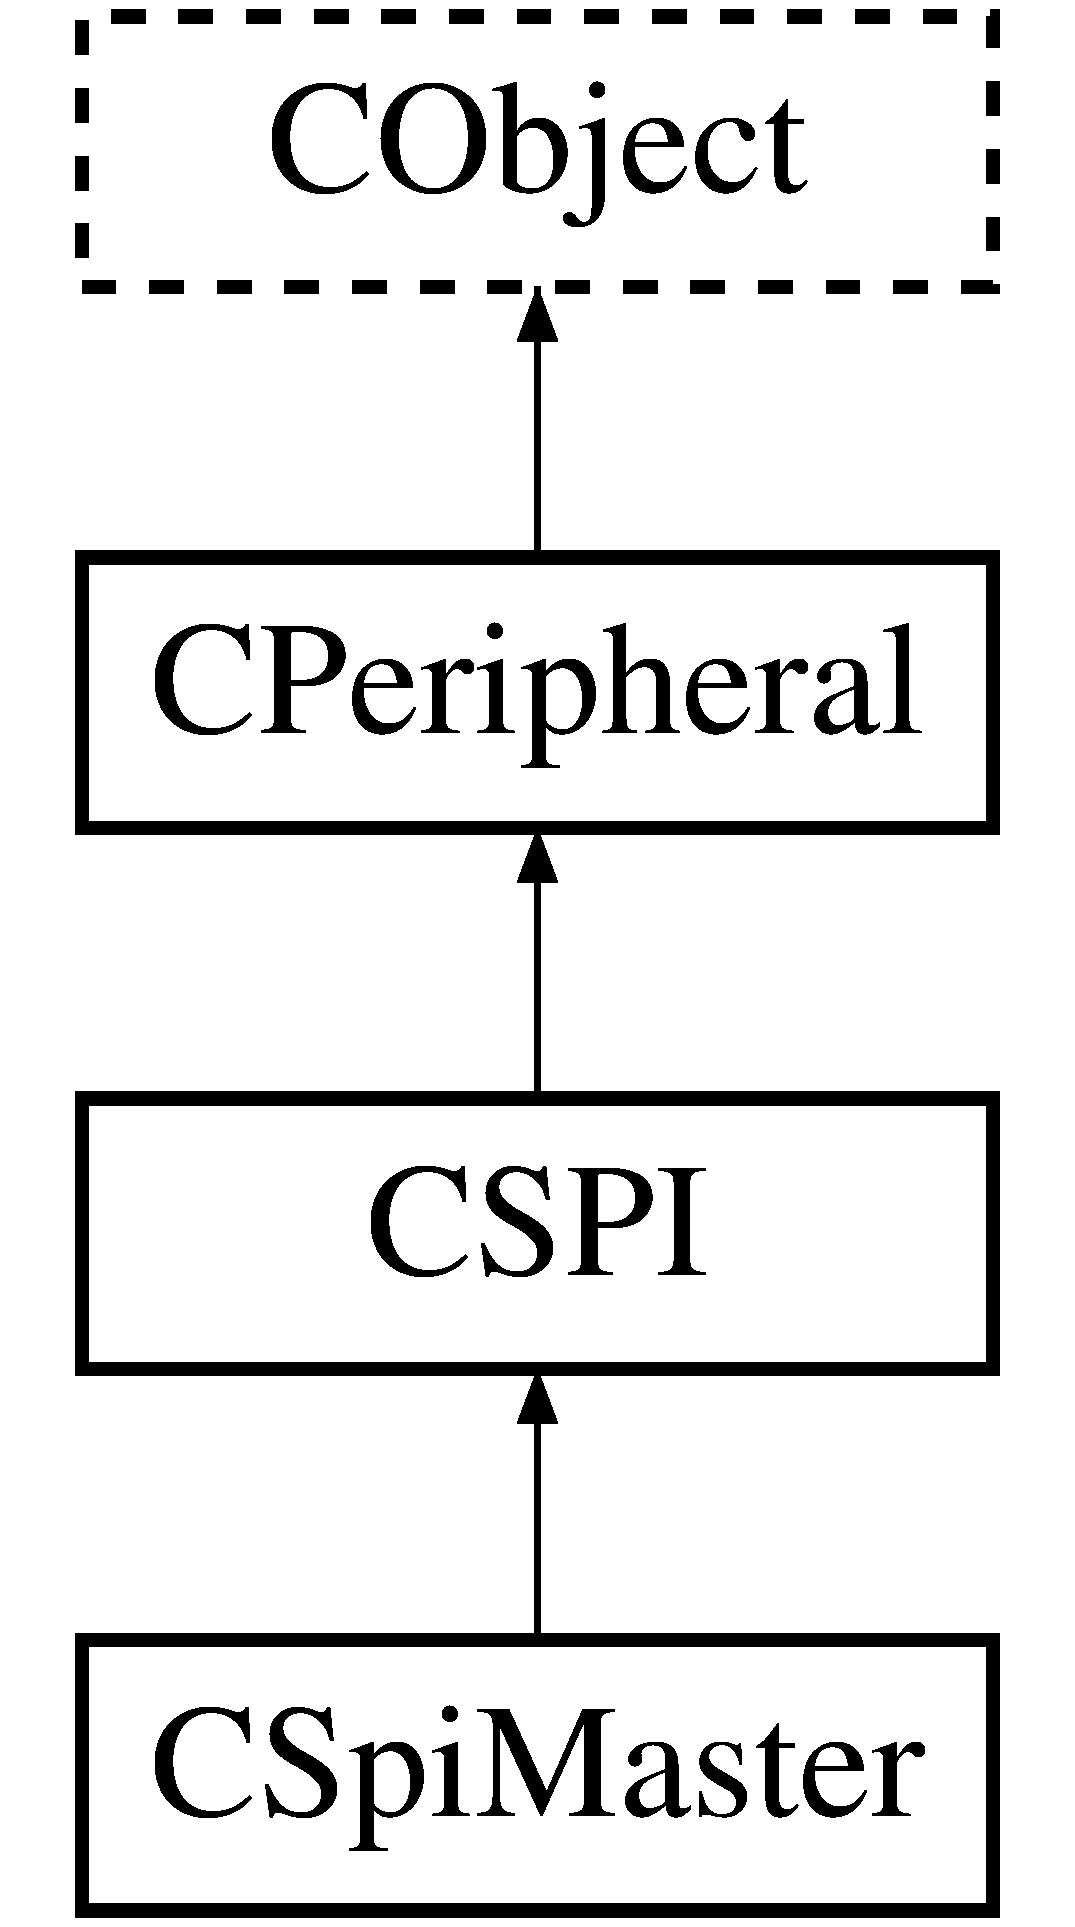
\includegraphics[height=4.000000cm]{d9/d9b/class_c_spi_master}
\end{center}
\end{figure}
\subsection*{Public Member Functions}
\begin{DoxyCompactItemize}
\item 
\hyperlink{class_c_spi_master_ae8d9da2cee5e13a06c8ed5e4146e4800}{C\-Spi\-Master} (P\-I\-N\-\_\-\-N\-A\-M\-E\-\_\-\-T sel\-Pin)
\item 
virtual int \hyperlink{class_c_spi_master_a13d1514765c41561d16dd46eefb9926e}{readwrite} (void $\ast$txbuf, void $\ast$rxbuf, uint32\-\_\-t length)
\end{DoxyCompactItemize}
\subsection*{Protected Attributes}
\begin{DoxyCompactItemize}
\item 
\hyperlink{class_c_pin}{C\-Pin} \hyperlink{class_c_spi_master_aee50dcd7bb052ad758e8bb5bf0362eb4}{m\-\_\-cs}
\end{DoxyCompactItemize}


\subsection{Constructor \& Destructor Documentation}
\hypertarget{class_c_spi_master_ae8d9da2cee5e13a06c8ed5e4146e4800}{\index{C\-Spi\-Master@{C\-Spi\-Master}!C\-Spi\-Master@{C\-Spi\-Master}}
\index{C\-Spi\-Master@{C\-Spi\-Master}!CSpiMaster@{C\-Spi\-Master}}
\subsubsection[{C\-Spi\-Master}]{\setlength{\rightskip}{0pt plus 5cm}C\-Spi\-Master\-::\-C\-Spi\-Master (
\begin{DoxyParamCaption}
\item[{P\-I\-N\-\_\-\-N\-A\-M\-E\-\_\-\-T}]{sel\-Pin}
\end{DoxyParamCaption}
)}}\label{class_c_spi_master_ae8d9da2cee5e13a06c8ed5e4146e4800}


\subsection{Member Function Documentation}
\hypertarget{class_c_spi_master_a13d1514765c41561d16dd46eefb9926e}{\index{C\-Spi\-Master@{C\-Spi\-Master}!readwrite@{readwrite}}
\index{readwrite@{readwrite}!CSpiMaster@{C\-Spi\-Master}}
\subsubsection[{readwrite}]{\setlength{\rightskip}{0pt plus 5cm}virtual int C\-Spi\-Master\-::readwrite (
\begin{DoxyParamCaption}
\item[{void $\ast$}]{txbuf, }
\item[{void $\ast$}]{rxbuf, }
\item[{uint32\-\_\-t}]{length}
\end{DoxyParamCaption}
)\hspace{0.3cm}{\ttfamily [virtual]}}}\label{class_c_spi_master_a13d1514765c41561d16dd46eefb9926e}


Reimplemented from \hyperlink{class_c_s_p_i_a5215a320db4cb5f2792ea18f8d6e0671}{C\-S\-P\-I}.



\subsection{Member Data Documentation}
\hypertarget{class_c_spi_master_aee50dcd7bb052ad758e8bb5bf0362eb4}{\index{C\-Spi\-Master@{C\-Spi\-Master}!m\-\_\-cs@{m\-\_\-cs}}
\index{m\-\_\-cs@{m\-\_\-cs}!CSpiMaster@{C\-Spi\-Master}}
\subsubsection[{m\-\_\-cs}]{\setlength{\rightskip}{0pt plus 5cm}{\bf C\-Pin} C\-Spi\-Master\-::m\-\_\-cs\hspace{0.3cm}{\ttfamily [protected]}}}\label{class_c_spi_master_aee50dcd7bb052ad758e8bb5bf0362eb4}


The documentation for this class was generated from the following file\-:\begin{DoxyCompactItemize}
\item 
spi.\-h\end{DoxyCompactItemize}

\hypertarget{class_c_stream}{\section{C\-Stream Class Reference}
\label{class_c_stream}\index{C\-Stream@{C\-Stream}}
}


{\ttfamily \#include \char`\"{}class/stream.\-h\char`\"{}}

Inheritance diagram for C\-Stream\-:\begin{figure}[H]
\begin{center}
\leavevmode
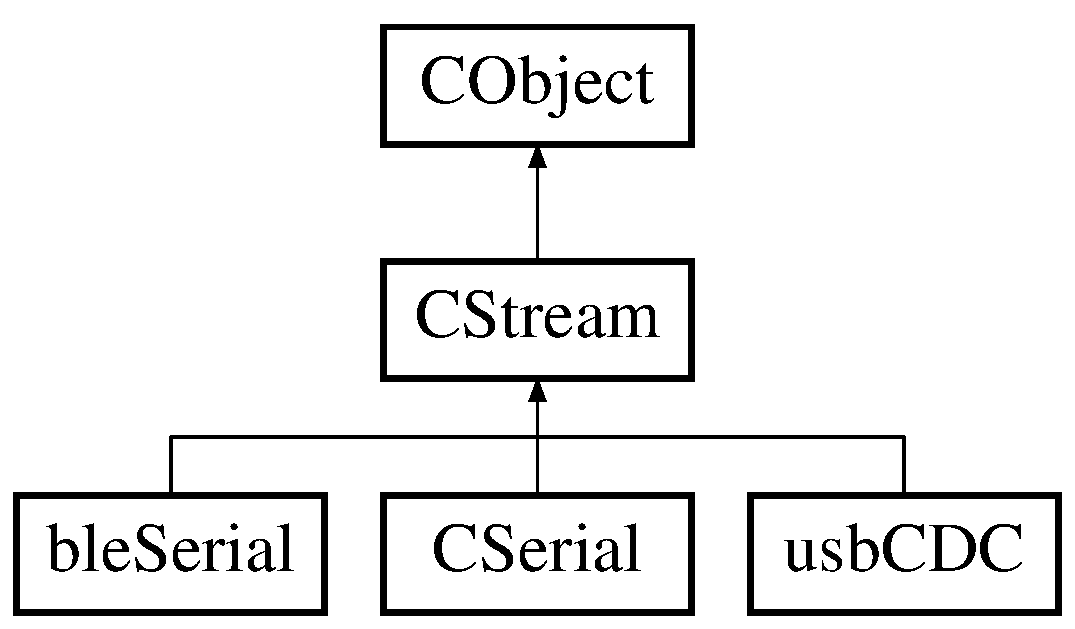
\includegraphics[height=3.000000cm]{d4/d16/class_c_stream}
\end{center}
\end{figure}
\subsection*{Public Member Functions}
\begin{DoxyCompactItemize}
\item 
\hyperlink{class_c_stream_acd9fd6c1ed458608829da8288047515c}{C\-Stream} ()
\item 
virtual \hyperlink{class_c_stream_ab1387be186f7dd1877455ea246b56d5e}{$\sim$\-C\-Stream} ()
\item 
virtual int \hyperlink{class_c_stream_a96328807241e15017868b845b06fd9e4}{readable} ()
\item 
virtual int \hyperlink{class_c_stream_a56ec27ee664f1a4eb9910988b78833d5}{writeable} ()
\item 
virtual int \hyperlink{class_c_stream_a80977482ffb2f7b626a9f29f437b7d8d}{read} (void $\ast$buf, int len, bool block=true)
\item 
virtual int \hyperlink{class_c_stream_a172fe857c74488b881007c65cc2e9552}{write} (const void $\ast$buf, int len, bool block=true)
\item 
virtual bool \hyperlink{class_c_stream_a7a152e6bda8654064634428d81bd81cb}{is\-Connected} ()
\item 
virtual void \hyperlink{class_c_stream_a5bd707b33627e01c2069b14bbf10694a}{flush} ()
\item 
int \hyperlink{class_c_stream_aa5c2d9723e67ba97a65a890f0b55656f}{write} (int ch)
\item 
int \hyperlink{class_c_stream_a59d24a785259d0f0aa3f8f44a1046fd7}{read} ()
\end{DoxyCompactItemize}


\subsection{Detailed Description}
An abstract class, to define the serial stream input and output interface. 

\subsection{Constructor \& Destructor Documentation}
\hypertarget{class_c_stream_acd9fd6c1ed458608829da8288047515c}{\index{C\-Stream@{C\-Stream}!C\-Stream@{C\-Stream}}
\index{C\-Stream@{C\-Stream}!CStream@{C\-Stream}}
\subsubsection[{C\-Stream}]{\setlength{\rightskip}{0pt plus 5cm}C\-Stream\-::\-C\-Stream (
\begin{DoxyParamCaption}
{}
\end{DoxyParamCaption}
)}}\label{class_c_stream_acd9fd6c1ed458608829da8288047515c}
\hyperlink{class_c_stream}{C\-Stream} constructor \hypertarget{class_c_stream_ab1387be186f7dd1877455ea246b56d5e}{\index{C\-Stream@{C\-Stream}!$\sim$\-C\-Stream@{$\sim$\-C\-Stream}}
\index{$\sim$\-C\-Stream@{$\sim$\-C\-Stream}!CStream@{C\-Stream}}
\subsubsection[{$\sim$\-C\-Stream}]{\setlength{\rightskip}{0pt plus 5cm}virtual C\-Stream\-::$\sim$\-C\-Stream (
\begin{DoxyParamCaption}
{}
\end{DoxyParamCaption}
)\hspace{0.3cm}{\ttfamily [virtual]}}}\label{class_c_stream_ab1387be186f7dd1877455ea246b56d5e}
\hyperlink{class_c_stream}{C\-Stream} destructor 

\subsection{Member Function Documentation}
\hypertarget{class_c_stream_a96328807241e15017868b845b06fd9e4}{\index{C\-Stream@{C\-Stream}!readable@{readable}}
\index{readable@{readable}!CStream@{C\-Stream}}
\subsubsection[{readable}]{\setlength{\rightskip}{0pt plus 5cm}virtual int C\-Stream\-::readable (
\begin{DoxyParamCaption}
{}
\end{DoxyParamCaption}
)\hspace{0.3cm}{\ttfamily [virtual]}}}\label{class_c_stream_a96328807241e15017868b845b06fd9e4}
Determine how many data bytes are available to read. \begin{DoxyReturn}{Returns}
A value to indicate how many data byte is available in the input buffer. 
\end{DoxyReturn}
\begin{DoxyRemark}{Remarks}
the pure virtual function have to implement by child class. 
\end{DoxyRemark}


Reimplemented in \hyperlink{classble_serial_a59dca8e3e2d6945a699347f4c4708fd4}{ble\-Serial}, \hyperlink{class_c_serial_a0748723f610ddcfdc34286dbbfbd4917}{C\-Serial}, and \hyperlink{classusb_c_d_c_a7182c4dfdad0293bba73a82056d43e80}{usb\-C\-D\-C}.

\hypertarget{class_c_stream_a56ec27ee664f1a4eb9910988b78833d5}{\index{C\-Stream@{C\-Stream}!writeable@{writeable}}
\index{writeable@{writeable}!CStream@{C\-Stream}}
\subsubsection[{writeable}]{\setlength{\rightskip}{0pt plus 5cm}virtual int C\-Stream\-::writeable (
\begin{DoxyParamCaption}
{}
\end{DoxyParamCaption}
)\hspace{0.3cm}{\ttfamily [virtual]}}}\label{class_c_stream_a56ec27ee664f1a4eb9910988b78833d5}
Determine how many data space are available to write. \begin{DoxyReturn}{Returns}
A value to indicate how many data space is available in the output buffer. 
\end{DoxyReturn}
\begin{DoxyRemark}{Remarks}
the pure virtual function have to implement by child class. 
\end{DoxyRemark}


Reimplemented in \hyperlink{classble_serial_ac42a8f805e6784e0fa2064270b5288a1}{ble\-Serial}, \hyperlink{class_c_serial_ac59cfe80216e1fb7eb479017f0bb8e7f}{C\-Serial}, and \hyperlink{classusb_c_d_c_ae45acb09392fedde912a5dba6fc3b88a}{usb\-C\-D\-C}.

\hypertarget{class_c_stream_a80977482ffb2f7b626a9f29f437b7d8d}{\index{C\-Stream@{C\-Stream}!read@{read}}
\index{read@{read}!CStream@{C\-Stream}}
\subsubsection[{read}]{\setlength{\rightskip}{0pt plus 5cm}virtual int C\-Stream\-::read (
\begin{DoxyParamCaption}
\item[{void $\ast$}]{buf, }
\item[{int}]{len, }
\item[{bool}]{block = {\ttfamily true}}
\end{DoxyParamCaption}
)\hspace{0.3cm}{\ttfamily [virtual]}}}\label{class_c_stream_a80977482ffb2f7b626a9f29f437b7d8d}
To read the stream to buffer. 
\begin{DoxyParams}[1]{Parameters}
\mbox{\tt in}  & {\em buf} & Destination buffer. \\
\hline
\mbox{\tt in}  & {\em len} & Length of destination buffer. \\
\hline
\mbox{\tt in}  & {\em block} & If true, to block in the read function unit to the indication length (len) be read. \\
\hline
\end{DoxyParams}
\begin{DoxyReturn}{Returns}
A value to indicate how many data bytes to read. 
\end{DoxyReturn}
\begin{DoxyRemark}{Remarks}
the pure virtual function have to implement by child class. 
\end{DoxyRemark}


Reimplemented in \hyperlink{classble_serial_a186e09706d9b6e58a6213ac0b6a220ad}{ble\-Serial}, \hyperlink{class_c_serial_a9b658bf4bc4d81413627bc2fe81e1471}{C\-Serial}, and \hyperlink{classusb_c_d_c_a65831ad4bfa85bf83f467c63b9f22799}{usb\-C\-D\-C}.

\hypertarget{class_c_stream_a172fe857c74488b881007c65cc2e9552}{\index{C\-Stream@{C\-Stream}!write@{write}}
\index{write@{write}!CStream@{C\-Stream}}
\subsubsection[{write}]{\setlength{\rightskip}{0pt plus 5cm}virtual int C\-Stream\-::write (
\begin{DoxyParamCaption}
\item[{const void $\ast$}]{buf, }
\item[{int}]{len, }
\item[{bool}]{block = {\ttfamily true}}
\end{DoxyParamCaption}
)\hspace{0.3cm}{\ttfamily [virtual]}}}\label{class_c_stream_a172fe857c74488b881007c65cc2e9552}
To write the buffer to stream. 
\begin{DoxyParams}[1]{Parameters}
\mbox{\tt out}  & {\em buf} & Source buffer. \\
\hline
\mbox{\tt in}  & {\em len} & Length of source buffer. \\
\hline
\mbox{\tt in}  & {\em block} & If true, to block in the write function unit to the indication length (len) be sent. \\
\hline
\end{DoxyParams}
\begin{DoxyReturn}{Returns}
A value to indicate how many data bytes to write. 
\end{DoxyReturn}
\begin{DoxyRemark}{Remarks}
the pure virtual function have to implement by child class. 
\end{DoxyRemark}


Reimplemented in \hyperlink{classble_serial_ab9d147e7dcb9436f390f2ad29d539930}{ble\-Serial}, \hyperlink{class_c_serial_adef6d3e77843c65617b7cb555c2f8732}{C\-Serial}, and \hyperlink{classusb_c_d_c_a340c728ca722a61a3a457a546a301dec}{usb\-C\-D\-C}.

\hypertarget{class_c_stream_a7a152e6bda8654064634428d81bd81cb}{\index{C\-Stream@{C\-Stream}!is\-Connected@{is\-Connected}}
\index{is\-Connected@{is\-Connected}!CStream@{C\-Stream}}
\subsubsection[{is\-Connected}]{\setlength{\rightskip}{0pt plus 5cm}virtual bool C\-Stream\-::is\-Connected (
\begin{DoxyParamCaption}
{}
\end{DoxyParamCaption}
)\hspace{0.3cm}{\ttfamily [virtual]}}}\label{class_c_stream_a7a152e6bda8654064634428d81bd81cb}
Check the current connection is valid or not. \begin{DoxyReturn}{Returns}
true if current connection is valid. 
\end{DoxyReturn}
\begin{DoxyRemark}{Remarks}
the pure virtual function have to implement by child class. 
\end{DoxyRemark}


Reimplemented in \hyperlink{classble_serial_aebfde0d9a7583cb641ac60f02df7cd77}{ble\-Serial}, \hyperlink{class_c_serial_ae7c133c4586cd5ca729cd026f813a8a0}{C\-Serial}, and \hyperlink{classusb_c_d_c_a0c0cb27d108bed8763e68a4121efee32}{usb\-C\-D\-C}.

\hypertarget{class_c_stream_a5bd707b33627e01c2069b14bbf10694a}{\index{C\-Stream@{C\-Stream}!flush@{flush}}
\index{flush@{flush}!CStream@{C\-Stream}}
\subsubsection[{flush}]{\setlength{\rightskip}{0pt plus 5cm}virtual void C\-Stream\-::flush (
\begin{DoxyParamCaption}
{}
\end{DoxyParamCaption}
)\hspace{0.3cm}{\ttfamily [virtual]}}}\label{class_c_stream_a5bd707b33627e01c2069b14bbf10694a}
Flush the stream the both input and output buffer \begin{DoxyRemark}{Remarks}
the pure virtual function have to implement by child class. 
\end{DoxyRemark}


Reimplemented in \hyperlink{classble_serial_ad41b78cc1b0fc02ce65248147b32ffa8}{ble\-Serial}, \hyperlink{class_c_serial_a68aecf6351423ae0e8791870c9e694bf}{C\-Serial}, and \hyperlink{classusb_c_d_c_afebca0ce341d46537cc6e2a811bede72}{usb\-C\-D\-C}.

\hypertarget{class_c_stream_aa5c2d9723e67ba97a65a890f0b55656f}{\index{C\-Stream@{C\-Stream}!write@{write}}
\index{write@{write}!CStream@{C\-Stream}}
\subsubsection[{write}]{\setlength{\rightskip}{0pt plus 5cm}int C\-Stream\-::write (
\begin{DoxyParamCaption}
\item[{int}]{ch}
\end{DoxyParamCaption}
)\hspace{0.3cm}{\ttfamily [inline]}}}\label{class_c_stream_aa5c2d9723e67ba97a65a890f0b55656f}
An inline function to write a character to output buffer of stream. 
\begin{DoxyParams}{Parameters}
{\em ch} & is an integer data that will be send to the stream buffer, the data size is one byte. \\
\hline
\end{DoxyParams}
\begin{DoxyReturn}{Returns}
1 (length) if write successful, otherwise is fail. 
\end{DoxyReturn}
\begin{DoxyNote}{Note}
The inline function is a overload function to call to the \hyperlink{class_c_stream_a172fe857c74488b881007c65cc2e9552}{write()} member. 
\end{DoxyNote}
\hypertarget{class_c_stream_a59d24a785259d0f0aa3f8f44a1046fd7}{\index{C\-Stream@{C\-Stream}!read@{read}}
\index{read@{read}!CStream@{C\-Stream}}
\subsubsection[{read}]{\setlength{\rightskip}{0pt plus 5cm}int C\-Stream\-::read (
\begin{DoxyParamCaption}
{}
\end{DoxyParamCaption}
)\hspace{0.3cm}{\ttfamily [inline]}}}\label{class_c_stream_a59d24a785259d0f0aa3f8f44a1046fd7}
An inline function to read a character from input buffer of stream. \begin{DoxyReturn}{Returns}
the character value, the character size is one byte. 
\end{DoxyReturn}
\begin{DoxyNote}{Note}
The inline function is a overload function to call to the \hyperlink{class_c_stream_a59d24a785259d0f0aa3f8f44a1046fd7}{read()} member. 
\end{DoxyNote}


The documentation for this class was generated from the following file\-:\begin{DoxyCompactItemize}
\item 
stream.\-h\end{DoxyCompactItemize}

\hypertarget{class_c_string}{\section{C\-String Class Reference}
\label{class_c_string}\index{C\-String@{C\-String}}
}


a string class inherit from \hyperlink{class_c_small_printf}{C\-Small\-Printf}.  




{\ttfamily \#include \char`\"{}class/string.\-h\char`\"{}}

Inheritance diagram for C\-String\-:\begin{figure}[H]
\begin{center}
\leavevmode
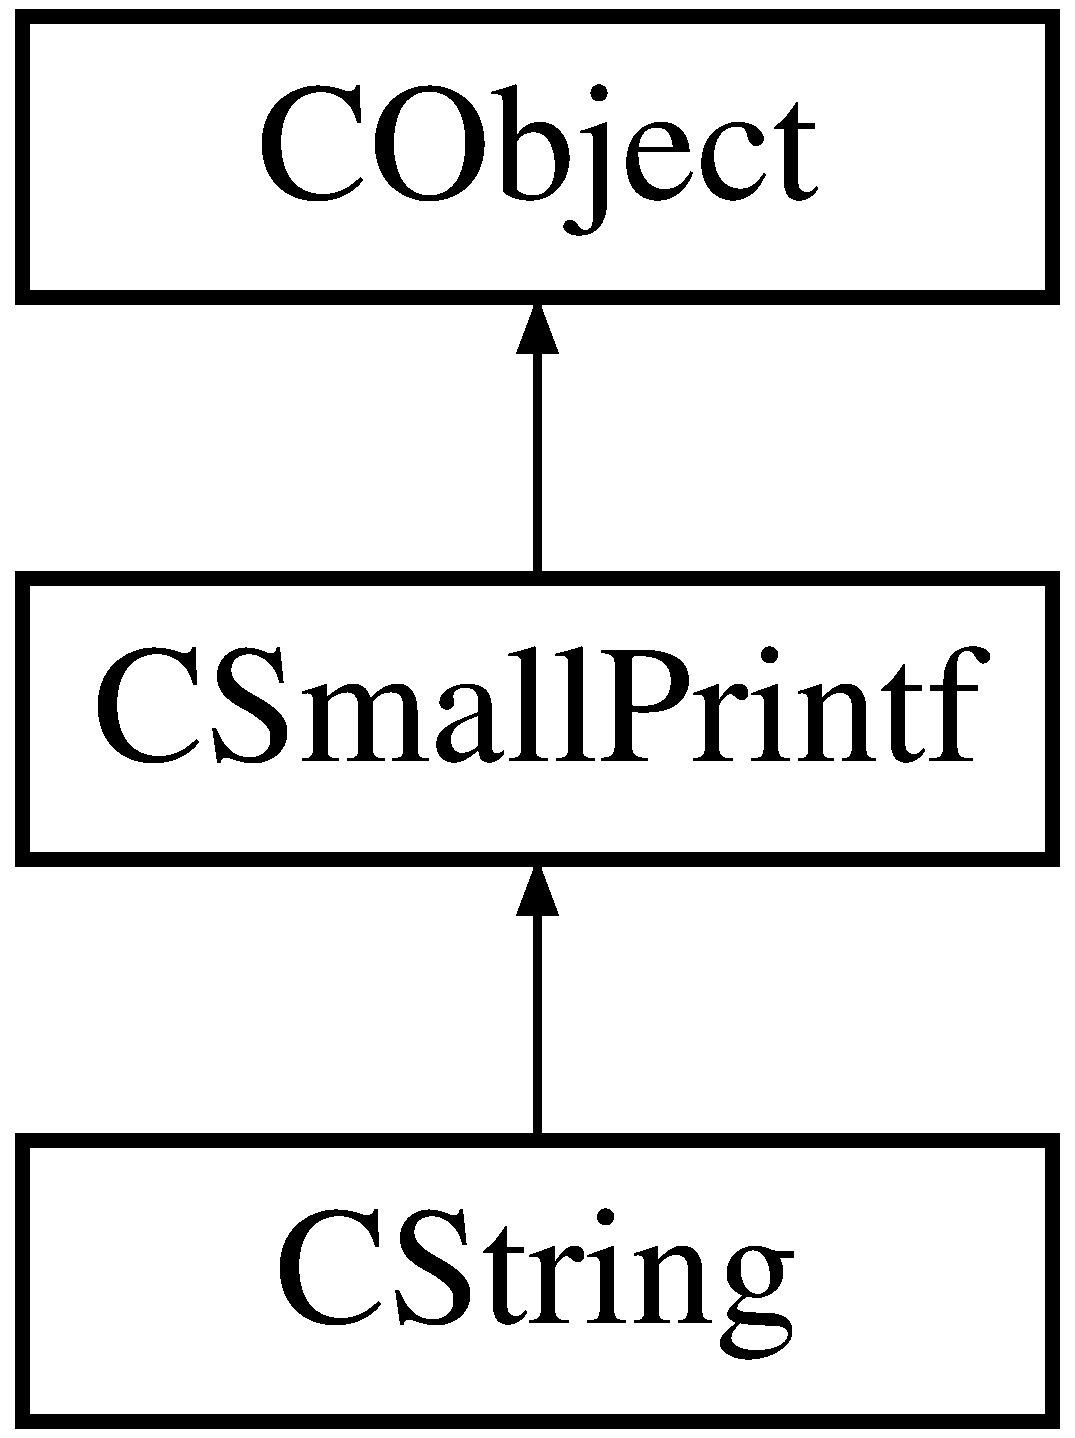
\includegraphics[height=3.000000cm]{df/d99/class_c_string}
\end{center}
\end{figure}
\subsection*{Public Member Functions}
\begin{DoxyCompactItemize}
\item 
\hyperlink{class_c_string_a3cb66b8f688676f29cdb51c914a15cf7}{C\-String} (int size=D\-E\-F\-\_\-\-S\-T\-R\-B\-U\-F\-\_\-\-S\-I\-Z\-E)
\item 
\hyperlink{class_c_string_a4866844f29a912ee7eb7afcb641ffb8f}{C\-String} (const \hyperlink{class_c_string}{C\-String} \&str)
\item 
\hyperlink{class_c_string_a233297b331dbc4c342745d67ad166b97}{C\-String} (L\-P\-C\-T\-S\-T\-R str, int \hyperlink{class_c_string_a8f131c0e097bea62d809acbc995807b9}{length}=0)
\item 
\hyperlink{class_c_string_a4cc7726fc9fbaa450876ffd98e3e6ff4}{C\-String} (L\-P\-T\-S\-T\-R buf)
\item 
virtual \hyperlink{class_c_string_a65b70fc602655e47340e5d8ae53167f3}{$\sim$\-C\-String} ()
\item 
virtual int \hyperlink{class_c_string_a1cc58a690ea6c9b8c4d7a9118fe3cc18}{get\-Buf\-Size} ()
\item 
virtual L\-P\-T\-S\-T\-R \hyperlink{class_c_string_ac7b886c37095673cc287d24100a9f3fd}{get\-Buffer} (bool lock=false)
\item 
virtual int \hyperlink{class_c_string_a5f5361665c7568d502d058992b14c016}{chk\-Length} ()
\item 
virtual void \hyperlink{class_c_string_a9cb7e6111fd46dd4d16a111ffe4af39d}{free\-Extra} ()
\item 
virtual int \hyperlink{class_c_string_a8f131c0e097bea62d809acbc995807b9}{length} ()
\item 
virtual void \hyperlink{class_c_string_a86bdac885b2d28689a62cbb6ae8b9ee4}{clear} ()
\item 
virtual T\-C\-H\-A\-R \hyperlink{class_c_string_ae1bcd2dd9d59762b41fe898916bfdd23}{get\-At} (int index)
\item 
virtual void \hyperlink{class_c_string_a99eaccef0daa453bf36ec886ae9b42c4}{set\-At} (int index, T\-C\-H\-A\-R ch)
\item 
virtual int \hyperlink{class_c_string_a181b18bf81568cee519617106706963f}{copy} (\hyperlink{class_c_string}{C\-String} \&str)
\item 
virtual int \hyperlink{class_c_string_a98fd9f07225ffd32a683d0ffe3e70bac}{copy} (L\-P\-C\-T\-S\-T\-R str, int \hyperlink{class_c_string_a8f131c0e097bea62d809acbc995807b9}{length})
\item 
virtual \hyperlink{class_c_string}{C\-String} \hyperlink{class_c_string_aeebb301ee8968688fd6ea8029a95ce9c}{clone} ()
\item 
virtual L\-P\-C\-T\-S\-T\-R \hyperlink{class_c_string_a7a027f50c1bede9a37d12ec9d2cc6616}{make\-Upper} ()
\item 
virtual L\-P\-C\-T\-S\-T\-R \hyperlink{class_c_string_af4236022a2befbcee7c1eaad21ba6798}{make\-Lower} ()
\item 
virtual L\-P\-C\-T\-S\-T\-R \hyperlink{class_c_string_a0b2512a4d0efb8c0317ef7a969268f07}{make\-Reverse} ()
\item 
virtual \hyperlink{class_c_string}{C\-String} \hyperlink{class_c_string_aae1e4a3db1f724363a300d706eae78b8}{mid} (int first, int count)
\item 
virtual int \hyperlink{class_c_string_a34ca981fe4599b24ed4312ee95a7f008}{find} (L\-P\-C\-T\-S\-T\-R str, int start=0)
\item 
virtual int \hyperlink{class_c_string_a225a9d464e22c27b750749426906c308}{find} (T\-C\-H\-A\-R ch, int start=0)
\item 
virtual int \hyperlink{class_c_string_a0d1d84239f8a01f8dd4e012fddc63cbe}{find\-I\-C} (L\-P\-C\-T\-S\-T\-R str, int start=0)
\item 
virtual int \hyperlink{class_c_string_a2330b9d10792cbf3dec9ccd747c67da1}{replace} (L\-P\-C\-T\-S\-T\-R oldstr, L\-P\-C\-T\-S\-T\-R newstr)
\item 
virtual int \hyperlink{class_c_string_aade923167835efe164b5e06fb192e176}{uri\-Decode} (L\-P\-C\-T\-S\-T\-R uri)
\item 
virtual T\-C\-H\-A\-R \hyperlink{class_c_string_a198badb5e4ffe29258ae2476836e274a}{operator\mbox{[}$\,$\mbox{]}} (int index)
\item 
virtual void \hyperlink{class_c_string_a68736847dab1a820326697c0321bce63}{operator=} (\hyperlink{class_c_string}{C\-String} \&str)
\item 
virtual void \hyperlink{class_c_string_a1ceee05f01a8bc4b96a25f0bfb3d9a2b}{operator=} (L\-P\-C\-T\-S\-T\-R str)
\item 
virtual \hyperlink{class_c_string}{C\-String} \& \hyperlink{class_c_string_ae4536c8c8913afaebdc72f79bbe02d9d}{operator+} (\hyperlink{class_c_string}{C\-String} \&str)
\item 
virtual \hyperlink{class_c_string}{C\-String} \& \hyperlink{class_c_string_a80701bf9d780b7cfa78930de18a54e5e}{operator+} (T\-C\-H\-A\-R ch)
\item 
virtual \hyperlink{class_c_string}{C\-String} \& \hyperlink{class_c_string_aed0a539d88caa84a10e42c56736b8585}{operator+} (L\-P\-C\-T\-S\-T\-R str)
\item 
virtual void \hyperlink{class_c_string_a40bc4b86a267617199efa1bd1b4054eb}{operator+=} (\hyperlink{class_c_string}{C\-String} \&str)
\item 
virtual void \hyperlink{class_c_string_aa65a2be961ede8c8894248c4d6faba79}{operator+=} (T\-C\-H\-A\-R ch)
\item 
virtual void \hyperlink{class_c_string_a776672751c58502039234d6c78832a9b}{operator+=} (L\-P\-C\-T\-S\-T\-R str)
\item 
virtual void \hyperlink{class_c_string_ad0593358c21cca96aca2403be6d6ec92}{operator+=} (int val)
\item 
virtual void \hyperlink{class_c_string_abee606394e7b160c90aaa492febecdee}{operator+=} (double val)
\item 
virtual void \hyperlink{class_c_string_a33449318e0ed01e0307993e1f173747f}{operator+=} (uint32\-\_\-t val)
\item 
virtual bool \hyperlink{class_c_string_a960b7b752e43ec86a0851e30fa9f5f16}{operator==} (\hyperlink{class_c_string}{C\-String} \&str)
\item 
virtual bool \hyperlink{class_c_string_a6aee7112647fd18a9161497494418e16}{operator==} (L\-P\-C\-T\-S\-T\-R str)
\item 
virtual L\-P\-C\-T\-S\-T\-R \hyperlink{class_c_string_aab798ff84e78c0bce521dad477bcdfa6}{operator$\ast$} ()
\item 
virtual \hyperlink{class_c_string_a9149db10490c1d9c4c969043877f3cdb}{operator L\-P\-C\-T\-S\-T\-R} ()
\end{DoxyCompactItemize}


\subsection{Detailed Description}
a string class inherit from \hyperlink{class_c_small_printf}{C\-Small\-Printf}. 

\subsection{Constructor \& Destructor Documentation}
\hypertarget{class_c_string_a3cb66b8f688676f29cdb51c914a15cf7}{\index{C\-String@{C\-String}!C\-String@{C\-String}}
\index{C\-String@{C\-String}!CString@{C\-String}}
\subsubsection[{C\-String}]{\setlength{\rightskip}{0pt plus 5cm}C\-String\-::\-C\-String (
\begin{DoxyParamCaption}
\item[{int}]{size = {\ttfamily DEF\-\_\-STRBUF\-\_\-SIZE}}
\end{DoxyParamCaption}
)}}\label{class_c_string_a3cb66b8f688676f29cdb51c914a15cf7}
\hypertarget{class_c_string_a4866844f29a912ee7eb7afcb641ffb8f}{\index{C\-String@{C\-String}!C\-String@{C\-String}}
\index{C\-String@{C\-String}!CString@{C\-String}}
\subsubsection[{C\-String}]{\setlength{\rightskip}{0pt plus 5cm}C\-String\-::\-C\-String (
\begin{DoxyParamCaption}
\item[{const {\bf C\-String} \&}]{str}
\end{DoxyParamCaption}
)}}\label{class_c_string_a4866844f29a912ee7eb7afcb641ffb8f}
\hypertarget{class_c_string_a233297b331dbc4c342745d67ad166b97}{\index{C\-String@{C\-String}!C\-String@{C\-String}}
\index{C\-String@{C\-String}!CString@{C\-String}}
\subsubsection[{C\-String}]{\setlength{\rightskip}{0pt plus 5cm}C\-String\-::\-C\-String (
\begin{DoxyParamCaption}
\item[{L\-P\-C\-T\-S\-T\-R}]{str, }
\item[{int}]{length = {\ttfamily 0}}
\end{DoxyParamCaption}
)}}\label{class_c_string_a233297b331dbc4c342745d67ad166b97}
\hypertarget{class_c_string_a4cc7726fc9fbaa450876ffd98e3e6ff4}{\index{C\-String@{C\-String}!C\-String@{C\-String}}
\index{C\-String@{C\-String}!CString@{C\-String}}
\subsubsection[{C\-String}]{\setlength{\rightskip}{0pt plus 5cm}C\-String\-::\-C\-String (
\begin{DoxyParamCaption}
\item[{L\-P\-T\-S\-T\-R}]{buf}
\end{DoxyParamCaption}
)}}\label{class_c_string_a4cc7726fc9fbaa450876ffd98e3e6ff4}
\hypertarget{class_c_string_a65b70fc602655e47340e5d8ae53167f3}{\index{C\-String@{C\-String}!$\sim$\-C\-String@{$\sim$\-C\-String}}
\index{$\sim$\-C\-String@{$\sim$\-C\-String}!CString@{C\-String}}
\subsubsection[{$\sim$\-C\-String}]{\setlength{\rightskip}{0pt plus 5cm}virtual C\-String\-::$\sim$\-C\-String (
\begin{DoxyParamCaption}
{}
\end{DoxyParamCaption}
)\hspace{0.3cm}{\ttfamily [virtual]}}}\label{class_c_string_a65b70fc602655e47340e5d8ae53167f3}


\subsection{Member Function Documentation}
\hypertarget{class_c_string_a1cc58a690ea6c9b8c4d7a9118fe3cc18}{\index{C\-String@{C\-String}!get\-Buf\-Size@{get\-Buf\-Size}}
\index{get\-Buf\-Size@{get\-Buf\-Size}!CString@{C\-String}}
\subsubsection[{get\-Buf\-Size}]{\setlength{\rightskip}{0pt plus 5cm}virtual int C\-String\-::get\-Buf\-Size (
\begin{DoxyParamCaption}
{}
\end{DoxyParamCaption}
)\hspace{0.3cm}{\ttfamily [virtual]}}}\label{class_c_string_a1cc58a690ea6c9b8c4d7a9118fe3cc18}
\hypertarget{class_c_string_ac7b886c37095673cc287d24100a9f3fd}{\index{C\-String@{C\-String}!get\-Buffer@{get\-Buffer}}
\index{get\-Buffer@{get\-Buffer}!CString@{C\-String}}
\subsubsection[{get\-Buffer}]{\setlength{\rightskip}{0pt plus 5cm}virtual L\-P\-T\-S\-T\-R C\-String\-::get\-Buffer (
\begin{DoxyParamCaption}
\item[{bool}]{lock = {\ttfamily false}}
\end{DoxyParamCaption}
)\hspace{0.3cm}{\ttfamily [virtual]}}}\label{class_c_string_ac7b886c37095673cc287d24100a9f3fd}
\hypertarget{class_c_string_a5f5361665c7568d502d058992b14c016}{\index{C\-String@{C\-String}!chk\-Length@{chk\-Length}}
\index{chk\-Length@{chk\-Length}!CString@{C\-String}}
\subsubsection[{chk\-Length}]{\setlength{\rightskip}{0pt plus 5cm}virtual int C\-String\-::chk\-Length (
\begin{DoxyParamCaption}
{}
\end{DoxyParamCaption}
)\hspace{0.3cm}{\ttfamily [virtual]}}}\label{class_c_string_a5f5361665c7568d502d058992b14c016}
\hypertarget{class_c_string_a9cb7e6111fd46dd4d16a111ffe4af39d}{\index{C\-String@{C\-String}!free\-Extra@{free\-Extra}}
\index{free\-Extra@{free\-Extra}!CString@{C\-String}}
\subsubsection[{free\-Extra}]{\setlength{\rightskip}{0pt plus 5cm}virtual void C\-String\-::free\-Extra (
\begin{DoxyParamCaption}
{}
\end{DoxyParamCaption}
)\hspace{0.3cm}{\ttfamily [virtual]}}}\label{class_c_string_a9cb7e6111fd46dd4d16a111ffe4af39d}
\hypertarget{class_c_string_a8f131c0e097bea62d809acbc995807b9}{\index{C\-String@{C\-String}!length@{length}}
\index{length@{length}!CString@{C\-String}}
\subsubsection[{length}]{\setlength{\rightskip}{0pt plus 5cm}virtual int C\-String\-::length (
\begin{DoxyParamCaption}
{}
\end{DoxyParamCaption}
)\hspace{0.3cm}{\ttfamily [virtual]}}}\label{class_c_string_a8f131c0e097bea62d809acbc995807b9}
\hypertarget{class_c_string_a86bdac885b2d28689a62cbb6ae8b9ee4}{\index{C\-String@{C\-String}!clear@{clear}}
\index{clear@{clear}!CString@{C\-String}}
\subsubsection[{clear}]{\setlength{\rightskip}{0pt plus 5cm}virtual void C\-String\-::clear (
\begin{DoxyParamCaption}
{}
\end{DoxyParamCaption}
)\hspace{0.3cm}{\ttfamily [virtual]}}}\label{class_c_string_a86bdac885b2d28689a62cbb6ae8b9ee4}
\hypertarget{class_c_string_ae1bcd2dd9d59762b41fe898916bfdd23}{\index{C\-String@{C\-String}!get\-At@{get\-At}}
\index{get\-At@{get\-At}!CString@{C\-String}}
\subsubsection[{get\-At}]{\setlength{\rightskip}{0pt plus 5cm}virtual T\-C\-H\-A\-R C\-String\-::get\-At (
\begin{DoxyParamCaption}
\item[{int}]{index}
\end{DoxyParamCaption}
)\hspace{0.3cm}{\ttfamily [virtual]}}}\label{class_c_string_ae1bcd2dd9d59762b41fe898916bfdd23}
\hypertarget{class_c_string_a99eaccef0daa453bf36ec886ae9b42c4}{\index{C\-String@{C\-String}!set\-At@{set\-At}}
\index{set\-At@{set\-At}!CString@{C\-String}}
\subsubsection[{set\-At}]{\setlength{\rightskip}{0pt plus 5cm}virtual void C\-String\-::set\-At (
\begin{DoxyParamCaption}
\item[{int}]{index, }
\item[{T\-C\-H\-A\-R}]{ch}
\end{DoxyParamCaption}
)\hspace{0.3cm}{\ttfamily [virtual]}}}\label{class_c_string_a99eaccef0daa453bf36ec886ae9b42c4}
\hypertarget{class_c_string_a181b18bf81568cee519617106706963f}{\index{C\-String@{C\-String}!copy@{copy}}
\index{copy@{copy}!CString@{C\-String}}
\subsubsection[{copy}]{\setlength{\rightskip}{0pt plus 5cm}virtual int C\-String\-::copy (
\begin{DoxyParamCaption}
\item[{{\bf C\-String} \&}]{str}
\end{DoxyParamCaption}
)\hspace{0.3cm}{\ttfamily [virtual]}}}\label{class_c_string_a181b18bf81568cee519617106706963f}
\hypertarget{class_c_string_a98fd9f07225ffd32a683d0ffe3e70bac}{\index{C\-String@{C\-String}!copy@{copy}}
\index{copy@{copy}!CString@{C\-String}}
\subsubsection[{copy}]{\setlength{\rightskip}{0pt plus 5cm}virtual int C\-String\-::copy (
\begin{DoxyParamCaption}
\item[{L\-P\-C\-T\-S\-T\-R}]{str, }
\item[{int}]{length}
\end{DoxyParamCaption}
)\hspace{0.3cm}{\ttfamily [virtual]}}}\label{class_c_string_a98fd9f07225ffd32a683d0ffe3e70bac}
\hypertarget{class_c_string_aeebb301ee8968688fd6ea8029a95ce9c}{\index{C\-String@{C\-String}!clone@{clone}}
\index{clone@{clone}!CString@{C\-String}}
\subsubsection[{clone}]{\setlength{\rightskip}{0pt plus 5cm}virtual {\bf C\-String} C\-String\-::clone (
\begin{DoxyParamCaption}
{}
\end{DoxyParamCaption}
)\hspace{0.3cm}{\ttfamily [virtual]}}}\label{class_c_string_aeebb301ee8968688fd6ea8029a95ce9c}
\hypertarget{class_c_string_a7a027f50c1bede9a37d12ec9d2cc6616}{\index{C\-String@{C\-String}!make\-Upper@{make\-Upper}}
\index{make\-Upper@{make\-Upper}!CString@{C\-String}}
\subsubsection[{make\-Upper}]{\setlength{\rightskip}{0pt plus 5cm}virtual L\-P\-C\-T\-S\-T\-R C\-String\-::make\-Upper (
\begin{DoxyParamCaption}
{}
\end{DoxyParamCaption}
)\hspace{0.3cm}{\ttfamily [virtual]}}}\label{class_c_string_a7a027f50c1bede9a37d12ec9d2cc6616}
\hypertarget{class_c_string_af4236022a2befbcee7c1eaad21ba6798}{\index{C\-String@{C\-String}!make\-Lower@{make\-Lower}}
\index{make\-Lower@{make\-Lower}!CString@{C\-String}}
\subsubsection[{make\-Lower}]{\setlength{\rightskip}{0pt plus 5cm}virtual L\-P\-C\-T\-S\-T\-R C\-String\-::make\-Lower (
\begin{DoxyParamCaption}
{}
\end{DoxyParamCaption}
)\hspace{0.3cm}{\ttfamily [virtual]}}}\label{class_c_string_af4236022a2befbcee7c1eaad21ba6798}
\hypertarget{class_c_string_a0b2512a4d0efb8c0317ef7a969268f07}{\index{C\-String@{C\-String}!make\-Reverse@{make\-Reverse}}
\index{make\-Reverse@{make\-Reverse}!CString@{C\-String}}
\subsubsection[{make\-Reverse}]{\setlength{\rightskip}{0pt plus 5cm}virtual L\-P\-C\-T\-S\-T\-R C\-String\-::make\-Reverse (
\begin{DoxyParamCaption}
{}
\end{DoxyParamCaption}
)\hspace{0.3cm}{\ttfamily [virtual]}}}\label{class_c_string_a0b2512a4d0efb8c0317ef7a969268f07}
\hypertarget{class_c_string_aae1e4a3db1f724363a300d706eae78b8}{\index{C\-String@{C\-String}!mid@{mid}}
\index{mid@{mid}!CString@{C\-String}}
\subsubsection[{mid}]{\setlength{\rightskip}{0pt plus 5cm}virtual {\bf C\-String} C\-String\-::mid (
\begin{DoxyParamCaption}
\item[{int}]{first, }
\item[{int}]{count}
\end{DoxyParamCaption}
)\hspace{0.3cm}{\ttfamily [virtual]}}}\label{class_c_string_aae1e4a3db1f724363a300d706eae78b8}
\hypertarget{class_c_string_a34ca981fe4599b24ed4312ee95a7f008}{\index{C\-String@{C\-String}!find@{find}}
\index{find@{find}!CString@{C\-String}}
\subsubsection[{find}]{\setlength{\rightskip}{0pt plus 5cm}virtual int C\-String\-::find (
\begin{DoxyParamCaption}
\item[{L\-P\-C\-T\-S\-T\-R}]{str, }
\item[{int}]{start = {\ttfamily 0}}
\end{DoxyParamCaption}
)\hspace{0.3cm}{\ttfamily [virtual]}}}\label{class_c_string_a34ca981fe4599b24ed4312ee95a7f008}
\hypertarget{class_c_string_a225a9d464e22c27b750749426906c308}{\index{C\-String@{C\-String}!find@{find}}
\index{find@{find}!CString@{C\-String}}
\subsubsection[{find}]{\setlength{\rightskip}{0pt plus 5cm}virtual int C\-String\-::find (
\begin{DoxyParamCaption}
\item[{T\-C\-H\-A\-R}]{ch, }
\item[{int}]{start = {\ttfamily 0}}
\end{DoxyParamCaption}
)\hspace{0.3cm}{\ttfamily [virtual]}}}\label{class_c_string_a225a9d464e22c27b750749426906c308}
\hypertarget{class_c_string_a0d1d84239f8a01f8dd4e012fddc63cbe}{\index{C\-String@{C\-String}!find\-I\-C@{find\-I\-C}}
\index{find\-I\-C@{find\-I\-C}!CString@{C\-String}}
\subsubsection[{find\-I\-C}]{\setlength{\rightskip}{0pt plus 5cm}virtual int C\-String\-::find\-I\-C (
\begin{DoxyParamCaption}
\item[{L\-P\-C\-T\-S\-T\-R}]{str, }
\item[{int}]{start = {\ttfamily 0}}
\end{DoxyParamCaption}
)\hspace{0.3cm}{\ttfamily [virtual]}}}\label{class_c_string_a0d1d84239f8a01f8dd4e012fddc63cbe}
\hypertarget{class_c_string_a2330b9d10792cbf3dec9ccd747c67da1}{\index{C\-String@{C\-String}!replace@{replace}}
\index{replace@{replace}!CString@{C\-String}}
\subsubsection[{replace}]{\setlength{\rightskip}{0pt plus 5cm}virtual int C\-String\-::replace (
\begin{DoxyParamCaption}
\item[{L\-P\-C\-T\-S\-T\-R}]{oldstr, }
\item[{L\-P\-C\-T\-S\-T\-R}]{newstr}
\end{DoxyParamCaption}
)\hspace{0.3cm}{\ttfamily [virtual]}}}\label{class_c_string_a2330b9d10792cbf3dec9ccd747c67da1}
\hypertarget{class_c_string_aade923167835efe164b5e06fb192e176}{\index{C\-String@{C\-String}!uri\-Decode@{uri\-Decode}}
\index{uri\-Decode@{uri\-Decode}!CString@{C\-String}}
\subsubsection[{uri\-Decode}]{\setlength{\rightskip}{0pt plus 5cm}virtual int C\-String\-::uri\-Decode (
\begin{DoxyParamCaption}
\item[{L\-P\-C\-T\-S\-T\-R}]{uri}
\end{DoxyParamCaption}
)\hspace{0.3cm}{\ttfamily [virtual]}}}\label{class_c_string_aade923167835efe164b5e06fb192e176}
\hypertarget{class_c_string_a198badb5e4ffe29258ae2476836e274a}{\index{C\-String@{C\-String}!operator\mbox{[}$\,$\mbox{]}@{operator[]}}
\index{operator\mbox{[}$\,$\mbox{]}@{operator[]}!CString@{C\-String}}
\subsubsection[{operator[]}]{\setlength{\rightskip}{0pt plus 5cm}virtual T\-C\-H\-A\-R C\-String\-::operator\mbox{[}$\,$\mbox{]} (
\begin{DoxyParamCaption}
\item[{int}]{index}
\end{DoxyParamCaption}
)\hspace{0.3cm}{\ttfamily [virtual]}}}\label{class_c_string_a198badb5e4ffe29258ae2476836e274a}
\hypertarget{class_c_string_a68736847dab1a820326697c0321bce63}{\index{C\-String@{C\-String}!operator=@{operator=}}
\index{operator=@{operator=}!CString@{C\-String}}
\subsubsection[{operator=}]{\setlength{\rightskip}{0pt plus 5cm}virtual void C\-String\-::operator= (
\begin{DoxyParamCaption}
\item[{{\bf C\-String} \&}]{str}
\end{DoxyParamCaption}
)\hspace{0.3cm}{\ttfamily [virtual]}}}\label{class_c_string_a68736847dab1a820326697c0321bce63}
\hypertarget{class_c_string_a1ceee05f01a8bc4b96a25f0bfb3d9a2b}{\index{C\-String@{C\-String}!operator=@{operator=}}
\index{operator=@{operator=}!CString@{C\-String}}
\subsubsection[{operator=}]{\setlength{\rightskip}{0pt plus 5cm}virtual void C\-String\-::operator= (
\begin{DoxyParamCaption}
\item[{L\-P\-C\-T\-S\-T\-R}]{str}
\end{DoxyParamCaption}
)\hspace{0.3cm}{\ttfamily [virtual]}}}\label{class_c_string_a1ceee05f01a8bc4b96a25f0bfb3d9a2b}
\hypertarget{class_c_string_ae4536c8c8913afaebdc72f79bbe02d9d}{\index{C\-String@{C\-String}!operator+@{operator+}}
\index{operator+@{operator+}!CString@{C\-String}}
\subsubsection[{operator+}]{\setlength{\rightskip}{0pt plus 5cm}virtual {\bf C\-String}\& C\-String\-::operator+ (
\begin{DoxyParamCaption}
\item[{{\bf C\-String} \&}]{str}
\end{DoxyParamCaption}
)\hspace{0.3cm}{\ttfamily [virtual]}}}\label{class_c_string_ae4536c8c8913afaebdc72f79bbe02d9d}
\hypertarget{class_c_string_a80701bf9d780b7cfa78930de18a54e5e}{\index{C\-String@{C\-String}!operator+@{operator+}}
\index{operator+@{operator+}!CString@{C\-String}}
\subsubsection[{operator+}]{\setlength{\rightskip}{0pt plus 5cm}virtual {\bf C\-String}\& C\-String\-::operator+ (
\begin{DoxyParamCaption}
\item[{T\-C\-H\-A\-R}]{ch}
\end{DoxyParamCaption}
)\hspace{0.3cm}{\ttfamily [virtual]}}}\label{class_c_string_a80701bf9d780b7cfa78930de18a54e5e}
\hypertarget{class_c_string_aed0a539d88caa84a10e42c56736b8585}{\index{C\-String@{C\-String}!operator+@{operator+}}
\index{operator+@{operator+}!CString@{C\-String}}
\subsubsection[{operator+}]{\setlength{\rightskip}{0pt plus 5cm}virtual {\bf C\-String}\& C\-String\-::operator+ (
\begin{DoxyParamCaption}
\item[{L\-P\-C\-T\-S\-T\-R}]{str}
\end{DoxyParamCaption}
)\hspace{0.3cm}{\ttfamily [virtual]}}}\label{class_c_string_aed0a539d88caa84a10e42c56736b8585}
\hypertarget{class_c_string_a40bc4b86a267617199efa1bd1b4054eb}{\index{C\-String@{C\-String}!operator+=@{operator+=}}
\index{operator+=@{operator+=}!CString@{C\-String}}
\subsubsection[{operator+=}]{\setlength{\rightskip}{0pt plus 5cm}virtual void C\-String\-::operator+= (
\begin{DoxyParamCaption}
\item[{{\bf C\-String} \&}]{str}
\end{DoxyParamCaption}
)\hspace{0.3cm}{\ttfamily [virtual]}}}\label{class_c_string_a40bc4b86a267617199efa1bd1b4054eb}
\hypertarget{class_c_string_aa65a2be961ede8c8894248c4d6faba79}{\index{C\-String@{C\-String}!operator+=@{operator+=}}
\index{operator+=@{operator+=}!CString@{C\-String}}
\subsubsection[{operator+=}]{\setlength{\rightskip}{0pt plus 5cm}virtual void C\-String\-::operator+= (
\begin{DoxyParamCaption}
\item[{T\-C\-H\-A\-R}]{ch}
\end{DoxyParamCaption}
)\hspace{0.3cm}{\ttfamily [virtual]}}}\label{class_c_string_aa65a2be961ede8c8894248c4d6faba79}
\hypertarget{class_c_string_a776672751c58502039234d6c78832a9b}{\index{C\-String@{C\-String}!operator+=@{operator+=}}
\index{operator+=@{operator+=}!CString@{C\-String}}
\subsubsection[{operator+=}]{\setlength{\rightskip}{0pt plus 5cm}virtual void C\-String\-::operator+= (
\begin{DoxyParamCaption}
\item[{L\-P\-C\-T\-S\-T\-R}]{str}
\end{DoxyParamCaption}
)\hspace{0.3cm}{\ttfamily [virtual]}}}\label{class_c_string_a776672751c58502039234d6c78832a9b}
\hypertarget{class_c_string_ad0593358c21cca96aca2403be6d6ec92}{\index{C\-String@{C\-String}!operator+=@{operator+=}}
\index{operator+=@{operator+=}!CString@{C\-String}}
\subsubsection[{operator+=}]{\setlength{\rightskip}{0pt plus 5cm}virtual void C\-String\-::operator+= (
\begin{DoxyParamCaption}
\item[{int}]{val}
\end{DoxyParamCaption}
)\hspace{0.3cm}{\ttfamily [inline]}, {\ttfamily [virtual]}}}\label{class_c_string_ad0593358c21cca96aca2403be6d6ec92}
\hypertarget{class_c_string_abee606394e7b160c90aaa492febecdee}{\index{C\-String@{C\-String}!operator+=@{operator+=}}
\index{operator+=@{operator+=}!CString@{C\-String}}
\subsubsection[{operator+=}]{\setlength{\rightskip}{0pt plus 5cm}virtual void C\-String\-::operator+= (
\begin{DoxyParamCaption}
\item[{double}]{val}
\end{DoxyParamCaption}
)\hspace{0.3cm}{\ttfamily [inline]}, {\ttfamily [virtual]}}}\label{class_c_string_abee606394e7b160c90aaa492febecdee}
\hypertarget{class_c_string_a33449318e0ed01e0307993e1f173747f}{\index{C\-String@{C\-String}!operator+=@{operator+=}}
\index{operator+=@{operator+=}!CString@{C\-String}}
\subsubsection[{operator+=}]{\setlength{\rightskip}{0pt plus 5cm}virtual void C\-String\-::operator+= (
\begin{DoxyParamCaption}
\item[{uint32\-\_\-t}]{val}
\end{DoxyParamCaption}
)\hspace{0.3cm}{\ttfamily [inline]}, {\ttfamily [virtual]}}}\label{class_c_string_a33449318e0ed01e0307993e1f173747f}
\hypertarget{class_c_string_a960b7b752e43ec86a0851e30fa9f5f16}{\index{C\-String@{C\-String}!operator==@{operator==}}
\index{operator==@{operator==}!CString@{C\-String}}
\subsubsection[{operator==}]{\setlength{\rightskip}{0pt plus 5cm}virtual bool C\-String\-::operator== (
\begin{DoxyParamCaption}
\item[{{\bf C\-String} \&}]{str}
\end{DoxyParamCaption}
)\hspace{0.3cm}{\ttfamily [virtual]}}}\label{class_c_string_a960b7b752e43ec86a0851e30fa9f5f16}
\hypertarget{class_c_string_a6aee7112647fd18a9161497494418e16}{\index{C\-String@{C\-String}!operator==@{operator==}}
\index{operator==@{operator==}!CString@{C\-String}}
\subsubsection[{operator==}]{\setlength{\rightskip}{0pt plus 5cm}virtual bool C\-String\-::operator== (
\begin{DoxyParamCaption}
\item[{L\-P\-C\-T\-S\-T\-R}]{str}
\end{DoxyParamCaption}
)\hspace{0.3cm}{\ttfamily [virtual]}}}\label{class_c_string_a6aee7112647fd18a9161497494418e16}
\hypertarget{class_c_string_aab798ff84e78c0bce521dad477bcdfa6}{\index{C\-String@{C\-String}!operator$\ast$@{operator$\ast$}}
\index{operator$\ast$@{operator$\ast$}!CString@{C\-String}}
\subsubsection[{operator$\ast$}]{\setlength{\rightskip}{0pt plus 5cm}virtual L\-P\-C\-T\-S\-T\-R C\-String\-::operator$\ast$ (
\begin{DoxyParamCaption}
{}
\end{DoxyParamCaption}
)\hspace{0.3cm}{\ttfamily [inline]}, {\ttfamily [virtual]}}}\label{class_c_string_aab798ff84e78c0bce521dad477bcdfa6}
\hypertarget{class_c_string_a9149db10490c1d9c4c969043877f3cdb}{\index{C\-String@{C\-String}!operator L\-P\-C\-T\-S\-T\-R@{operator L\-P\-C\-T\-S\-T\-R}}
\index{operator L\-P\-C\-T\-S\-T\-R@{operator L\-P\-C\-T\-S\-T\-R}!CString@{C\-String}}
\subsubsection[{operator L\-P\-C\-T\-S\-T\-R}]{\setlength{\rightskip}{0pt plus 5cm}virtual C\-String\-::operator L\-P\-C\-T\-S\-T\-R (
\begin{DoxyParamCaption}
{}
\end{DoxyParamCaption}
)\hspace{0.3cm}{\ttfamily [inline]}, {\ttfamily [virtual]}}}\label{class_c_string_a9149db10490c1d9c4c969043877f3cdb}


The documentation for this class was generated from the following file\-:\begin{DoxyCompactItemize}
\item 
string.\-h\end{DoxyCompactItemize}

\hypertarget{class_c_thread}{\section{C\-Thread Class Reference}
\label{class_c_thread}\index{C\-Thread@{C\-Thread}}
}


{\ttfamily \#include \char`\"{}class/thread.\-h\char`\"{}}

Inheritance diagram for C\-Thread\-:\begin{figure}[H]
\begin{center}
\leavevmode
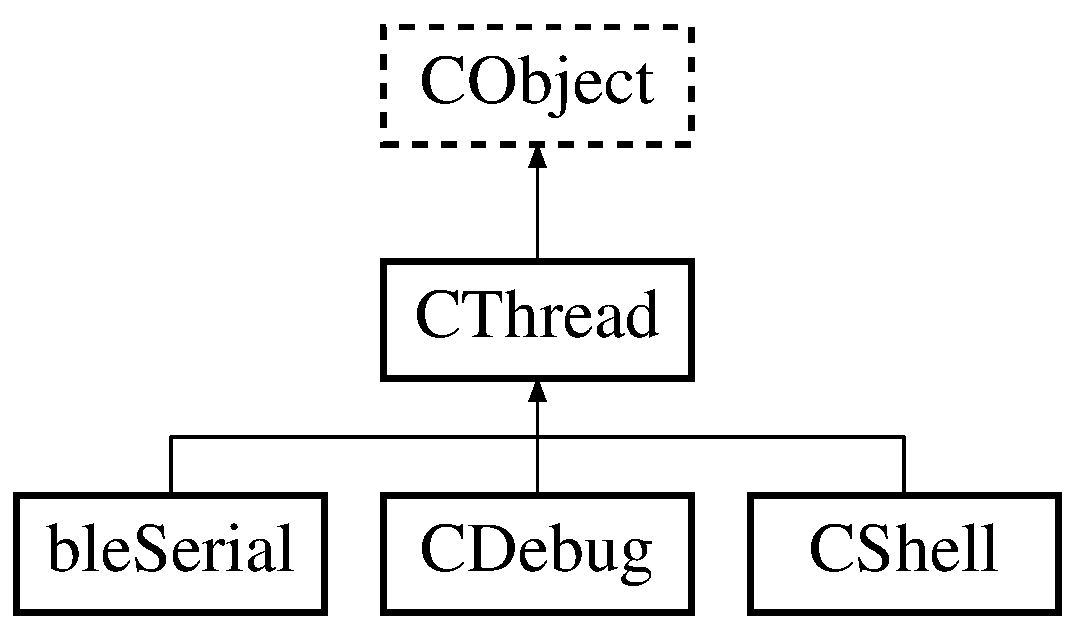
\includegraphics[height=3.000000cm]{d0/d26/class_c_thread}
\end{center}
\end{figure}
\subsection*{Public Member Functions}
\begin{DoxyCompactItemize}
\item 
virtual bool \hyperlink{class_c_thread_a3ebabcc071634508511ae2fc7b868ab7}{start} (const char $\ast$name, int stack=D\-E\-F\-\_\-\-T\-H\-R\-E\-A\-D\-\_\-\-S\-T\-A\-C\-K, \hyperlink{group___enumerations_ga51e24e4c0498282f564e92975e020c1d}{P\-R\-I\-O\-R\-I\-T\-I\-E\-S\-\_\-\-T} priority=\hyperlink{group___enumerations_gga51e24e4c0498282f564e92975e020c1daf8a2513dc9a78bb09c0520af65a3f402}{P\-R\-I\-\_\-\-L\-O\-W})
\item 
virtual bool \hyperlink{class_c_thread_aacf955d1852e74da1f989251955ee6ec}{start} ()
\item 
virtual void \hyperlink{class_c_thread_ac8c53aa8c145fc4ac70fa6d825b95742}{resume} ()
\item 
virtual void \hyperlink{class_c_thread_a53e71e6db2221cd1c45aec21953d4aad}{suspend} ()
\item 
uint32\-\_\-t \hyperlink{class_c_thread_ac0227eda51725b795a461a768703f588}{get\-Stack\-High\-Water\-Mark} ()
\item 
virtual bool \hyperlink{class_c_thread_a51dbe9909ce528b4113d2cc27314e965}{is\-Suspend} ()
\item 
\hyperlink{group___enumerations_ga25ee4013cc565a18ac2f4039b4ad441b}{T\-A\-S\-K\-\_\-\-S\-T\-A\-T\-E\-\_\-\-T} \hyperlink{class_c_thread_a1e9cce461d8dfb3889cea24f1a703f6f}{get\-State} ()
\item 
virtual void \hyperlink{class_c_thread_a6b0703ae0cc085a0c0aaa55b6945575b}{set\-Priority} (\hyperlink{group___enumerations_ga51e24e4c0498282f564e92975e020c1d}{P\-R\-I\-O\-R\-I\-T\-I\-E\-S\-\_\-\-T} p)
\item 
virtual \hyperlink{group___enumerations_ga51e24e4c0498282f564e92975e020c1d}{P\-R\-I\-O\-R\-I\-T\-I\-E\-S\-\_\-\-T} \hyperlink{class_c_thread_ac30b0a1f51549a97b88771692319c0e4}{get\-Priority} ()
\item 
L\-P\-C\-T\-S\-T\-R \hyperlink{class_c_thread_aa291909bc3ff7cc0decf46c885a7a725}{get\-Name} ()
\item 
virtual bool \hyperlink{class_c_thread_a4a0f0727be4714cef1e24150a869d403}{is\-Alive} ()
\item 
virtual void \hyperlink{class_c_thread_a15041136818470124d097d790d55a6e5}{kill} ()
\item 
virtual bool \hyperlink{class_c_thread_ab2513fd0fcad30e2e6605609c91f1984}{is\-Thread} ()
\end{DoxyCompactItemize}
\subsection*{Static Public Member Functions}
\begin{DoxyCompactItemize}
\item 
static void \hyperlink{class_c_thread_a743d4325b7e7da494283f3292773ff77}{resume\-All} ()
\item 
static void \hyperlink{class_c_thread_a2c09328581bd4e4a3e9e793f3376a92a}{suspend\-All} ()
\item 
static void \hyperlink{class_c_thread_aeb4cafe42d6cfc41294cf5dedcee8678}{enter\-Critical\-Section} ()
\item 
static void \hyperlink{class_c_thread_aab3a51062666552690be49b8e8027161}{exit\-Critical\-Section} ()
\end{DoxyCompactItemize}
\subsection*{Protected Member Functions}
\begin{DoxyCompactItemize}
\item 
virtual void \hyperlink{class_c_thread_a071c3d3b3c19a7bd6a01aca073a9b4d7}{run} ()
\end{DoxyCompactItemize}
\subsection*{Protected Attributes}
\begin{DoxyCompactItemize}
\item 
uint32\-\_\-t \hyperlink{class_c_thread_a2723c18f3f7659cdd93610fd1654d564}{m\-\_\-flag}
\end{DoxyCompactItemize}


\subsection{Detailed Description}
The \hyperlink{class_c_thread}{C\-Thread} class provide the multi-\/tasking services. \begin{DoxyNote}{Note}
The \hyperlink{class_c_thread}{C\-Thread} class is an abstract class, child class have to implement the \hyperlink{class_c_thread_a071c3d3b3c19a7bd6a01aca073a9b4d7}{run()} member. 
\end{DoxyNote}


\subsection{Member Function Documentation}
\hypertarget{class_c_thread_a3ebabcc071634508511ae2fc7b868ab7}{\index{C\-Thread@{C\-Thread}!start@{start}}
\index{start@{start}!CThread@{C\-Thread}}
\subsubsection[{start}]{\setlength{\rightskip}{0pt plus 5cm}virtual bool C\-Thread\-::start (
\begin{DoxyParamCaption}
\item[{const char $\ast$}]{name, }
\item[{int}]{stack = {\ttfamily DEF\-\_\-THREAD\-\_\-STACK}, }
\item[{{\bf P\-R\-I\-O\-R\-I\-T\-I\-E\-S\-\_\-\-T}}]{priority = {\ttfamily {\bf P\-R\-I\-\_\-\-L\-O\-W}}}
\end{DoxyParamCaption}
)\hspace{0.3cm}{\ttfamily [virtual]}}}\label{class_c_thread_a3ebabcc071634508511ae2fc7b868ab7}
Call the member function to start the thread. 
\begin{DoxyParams}{Parameters}
{\em name} & is a descriptive name for the task. \\
\hline
{\em stack} & is a integer value to specified as the number of stack can hold-\/not the number of bytes. \\
\hline
{\em priority} & at which the task should run. \\
\hline
\end{DoxyParams}
\begin{DoxyReturn}{Returns}
true if successful; otherwise, crate task failed.
\end{DoxyReturn}

\begin{DoxyCode}
Example:
        \textcolor{keyword}{class }CLedTask: \textcolor{keyword}{public} \hyperlink{class_c_thread}{CThread} \{
        \textcolor{keyword}{protected}:
            \textcolor{keyword}{virtual} \textcolor{keywordtype}{void} \hyperlink{class_c_thread_a071c3d3b3c19a7bd6a01aca073a9b4d7}{run}() \{
                \hyperlink{class_c_pin}{CPin} led(\hyperlink{group___enumerations_gga65a2241721e4acb573e0c3fe29ac432fa8379bbaa96d151e6adac488b2a147b7a}{LED2});
                \textcolor{keywordflow}{while}( \hyperlink{class_c_thread_a4a0f0727be4714cef1e24150a869d403}{isAlive}() ) \{    \textcolor{comment}{// Is thread in alive?  (when thread be kill, the isAlive
       will return false)}
                    led = !led;
                    sleep(200);
                \}
            \}
        \};

        \textcolor{keywordtype}{int} main() \{
            ...
            CLedTask ledTask;
            ledTask.start(\textcolor{stringliteral}{"led"});   \textcolor{comment}{// default stack=128, default priority=low}
            ...
        \}
\end{DoxyCode}
 \hypertarget{class_c_thread_aacf955d1852e74da1f989251955ee6ec}{\index{C\-Thread@{C\-Thread}!start@{start}}
\index{start@{start}!CThread@{C\-Thread}}
\subsubsection[{start}]{\setlength{\rightskip}{0pt plus 5cm}virtual bool C\-Thread\-::start (
\begin{DoxyParamCaption}
{}
\end{DoxyParamCaption}
)\hspace{0.3cm}{\ttfamily [virtual]}}}\label{class_c_thread_aacf955d1852e74da1f989251955ee6ec}
Call the member function to start the thread. \begin{DoxyNote}{Note}
the \hyperlink{class_c_thread_aacf955d1852e74da1f989251955ee6ec}{start()} is an overload member function of \hyperlink{class_c_thread}{C\-Thread}. 
\end{DoxyNote}


Reimplemented in \hyperlink{class_c_debug_a40d1b7f50b76311b3a7fb148e5b7e2ea}{C\-Debug}, and \hyperlink{class_c_shell_a670f66f552494dfce94ee297ae0f659a}{C\-Shell}.

\hypertarget{class_c_thread_ac8c53aa8c145fc4ac70fa6d825b95742}{\index{C\-Thread@{C\-Thread}!resume@{resume}}
\index{resume@{resume}!CThread@{C\-Thread}}
\subsubsection[{resume}]{\setlength{\rightskip}{0pt plus 5cm}virtual void C\-Thread\-::resume (
\begin{DoxyParamCaption}
{}
\end{DoxyParamCaption}
)\hspace{0.3cm}{\ttfamily [virtual]}}}\label{class_c_thread_ac8c53aa8c145fc4ac70fa6d825b95742}
Call the member function to resume the thread.


\begin{DoxyCode}
Example:
    \textcolor{keywordtype}{int} main() \{
        ...
        CLedTask ledTask;
        ledTask.start(\textcolor{stringliteral}{"led"});
        ...
        ledTask.suspend();      \textcolor{comment}{// suspend the ledTask}
        ...
        \textcolor{keywordflow}{if} ( ledTask.isSuspend() ) \{
            ledTask.resume();   \textcolor{comment}{// resume the ledTask}
        \}
        ...
    \}
\end{DoxyCode}
 \hypertarget{class_c_thread_a53e71e6db2221cd1c45aec21953d4aad}{\index{C\-Thread@{C\-Thread}!suspend@{suspend}}
\index{suspend@{suspend}!CThread@{C\-Thread}}
\subsubsection[{suspend}]{\setlength{\rightskip}{0pt plus 5cm}virtual void C\-Thread\-::suspend (
\begin{DoxyParamCaption}
{}
\end{DoxyParamCaption}
)\hspace{0.3cm}{\ttfamily [virtual]}}}\label{class_c_thread_a53e71e6db2221cd1c45aec21953d4aad}
Call the member function to suspend the thread.


\begin{DoxyCode}
Example:
    \textcolor{keywordtype}{int} main() \{
        ...
        CLedTask ledTask;
        ledTask.start(\textcolor{stringliteral}{"led"});
        ...
        ledTask.suspend();      \textcolor{comment}{// suspend the ledTask}
        ...
        \textcolor{keywordflow}{if} ( ledTask.isSuspend() ) \{
            ledTask.resume();   \textcolor{comment}{// resume the ledTask}
        \}
        ...
    \}
\end{DoxyCode}
 \hypertarget{class_c_thread_ac0227eda51725b795a461a768703f588}{\index{C\-Thread@{C\-Thread}!get\-Stack\-High\-Water\-Mark@{get\-Stack\-High\-Water\-Mark}}
\index{get\-Stack\-High\-Water\-Mark@{get\-Stack\-High\-Water\-Mark}!CThread@{C\-Thread}}
\subsubsection[{get\-Stack\-High\-Water\-Mark}]{\setlength{\rightskip}{0pt plus 5cm}uint32\-\_\-t C\-Thread\-::get\-Stack\-High\-Water\-Mark (
\begin{DoxyParamCaption}
{}
\end{DoxyParamCaption}
)}}\label{class_c_thread_ac0227eda51725b795a461a768703f588}
Call the member function to check the stack high water mark. \begin{DoxyNote}{Note}
Or use the shell and type 'task' to check all tasks status. 
\end{DoxyNote}
\hypertarget{class_c_thread_a51dbe9909ce528b4113d2cc27314e965}{\index{C\-Thread@{C\-Thread}!is\-Suspend@{is\-Suspend}}
\index{is\-Suspend@{is\-Suspend}!CThread@{C\-Thread}}
\subsubsection[{is\-Suspend}]{\setlength{\rightskip}{0pt plus 5cm}virtual bool C\-Thread\-::is\-Suspend (
\begin{DoxyParamCaption}
{}
\end{DoxyParamCaption}
)\hspace{0.3cm}{\ttfamily [virtual]}}}\label{class_c_thread_a51dbe9909ce528b4113d2cc27314e965}
Call the member function to check the task is in suspended or not. \begin{DoxyReturn}{Returns}
true if task in suspended. otherwise, the task in running. 
\end{DoxyReturn}
\hypertarget{class_c_thread_a1e9cce461d8dfb3889cea24f1a703f6f}{\index{C\-Thread@{C\-Thread}!get\-State@{get\-State}}
\index{get\-State@{get\-State}!CThread@{C\-Thread}}
\subsubsection[{get\-State}]{\setlength{\rightskip}{0pt plus 5cm}{\bf T\-A\-S\-K\-\_\-\-S\-T\-A\-T\-E\-\_\-\-T} C\-Thread\-::get\-State (
\begin{DoxyParamCaption}
{}
\end{DoxyParamCaption}
)}}\label{class_c_thread_a1e9cce461d8dfb3889cea24f1a703f6f}
Retrieve the state of thread object (task) \hypertarget{class_c_thread_a6b0703ae0cc085a0c0aaa55b6945575b}{\index{C\-Thread@{C\-Thread}!set\-Priority@{set\-Priority}}
\index{set\-Priority@{set\-Priority}!CThread@{C\-Thread}}
\subsubsection[{set\-Priority}]{\setlength{\rightskip}{0pt plus 5cm}virtual void C\-Thread\-::set\-Priority (
\begin{DoxyParamCaption}
\item[{{\bf P\-R\-I\-O\-R\-I\-T\-I\-E\-S\-\_\-\-T}}]{p}
\end{DoxyParamCaption}
)\hspace{0.3cm}{\ttfamily [virtual]}}}\label{class_c_thread_a6b0703ae0cc085a0c0aaa55b6945575b}
Call the member function to change the task's priority. 
\begin{DoxyParams}{Parameters}
{\em p} & is P\-R\-I\-O\-R\-I\-T\-I\-E\-S\-\_\-\-T to set a new priority for the task. \\
\hline
\end{DoxyParams}
\hypertarget{class_c_thread_ac30b0a1f51549a97b88771692319c0e4}{\index{C\-Thread@{C\-Thread}!get\-Priority@{get\-Priority}}
\index{get\-Priority@{get\-Priority}!CThread@{C\-Thread}}
\subsubsection[{get\-Priority}]{\setlength{\rightskip}{0pt plus 5cm}virtual {\bf P\-R\-I\-O\-R\-I\-T\-I\-E\-S\-\_\-\-T} C\-Thread\-::get\-Priority (
\begin{DoxyParamCaption}
{}
\end{DoxyParamCaption}
)\hspace{0.3cm}{\ttfamily [virtual]}}}\label{class_c_thread_ac30b0a1f51549a97b88771692319c0e4}
Call the member function to get the task's priority. \begin{DoxyReturn}{Returns}
P\-R\-I\-O\-R\-I\-T\-I\-E\-S\-\_\-\-T 
\end{DoxyReturn}
\hypertarget{class_c_thread_aa291909bc3ff7cc0decf46c885a7a725}{\index{C\-Thread@{C\-Thread}!get\-Name@{get\-Name}}
\index{get\-Name@{get\-Name}!CThread@{C\-Thread}}
\subsubsection[{get\-Name}]{\setlength{\rightskip}{0pt plus 5cm}L\-P\-C\-T\-S\-T\-R C\-Thread\-::get\-Name (
\begin{DoxyParamCaption}
{}
\end{DoxyParamCaption}
)}}\label{class_c_thread_aa291909bc3ff7cc0decf46c885a7a725}
Call the member function to retrieve the task's name. \hypertarget{class_c_thread_a4a0f0727be4714cef1e24150a869d403}{\index{C\-Thread@{C\-Thread}!is\-Alive@{is\-Alive}}
\index{is\-Alive@{is\-Alive}!CThread@{C\-Thread}}
\subsubsection[{is\-Alive}]{\setlength{\rightskip}{0pt plus 5cm}virtual bool C\-Thread\-::is\-Alive (
\begin{DoxyParamCaption}
{}
\end{DoxyParamCaption}
)\hspace{0.3cm}{\ttfamily [virtual]}}}\label{class_c_thread_a4a0f0727be4714cef1e24150a869d403}
is\-Alive is to check the thread is in alive (for run-\/loop) \hypertarget{class_c_thread_a15041136818470124d097d790d55a6e5}{\index{C\-Thread@{C\-Thread}!kill@{kill}}
\index{kill@{kill}!CThread@{C\-Thread}}
\subsubsection[{kill}]{\setlength{\rightskip}{0pt plus 5cm}virtual void C\-Thread\-::kill (
\begin{DoxyParamCaption}
{}
\end{DoxyParamCaption}
)\hspace{0.3cm}{\ttfamily [virtual]}}}\label{class_c_thread_a15041136818470124d097d790d55a6e5}
kill the thread, call the kill the \hyperlink{class_c_thread_a4a0f0727be4714cef1e24150a869d403}{is\-Alive()} will return false \hypertarget{class_c_thread_ab2513fd0fcad30e2e6605609c91f1984}{\index{C\-Thread@{C\-Thread}!is\-Thread@{is\-Thread}}
\index{is\-Thread@{is\-Thread}!CThread@{C\-Thread}}
\subsubsection[{is\-Thread}]{\setlength{\rightskip}{0pt plus 5cm}virtual bool C\-Thread\-::is\-Thread (
\begin{DoxyParamCaption}
{}
\end{DoxyParamCaption}
)\hspace{0.3cm}{\ttfamily [inline]}, {\ttfamily [virtual]}}}\label{class_c_thread_ab2513fd0fcad30e2e6605609c91f1984}
\hyperlink{class_c_thread_ab2513fd0fcad30e2e6605609c91f1984}{is\-Thread()}, check the class is inherited from \hyperlink{class_c_thread}{C\-Thread} 

Reimplemented from \hyperlink{class_c_object_a26a76c241a4d62d2efdac57d2cfe4c0f}{C\-Object}.

\hypertarget{class_c_thread_a743d4325b7e7da494283f3292773ff77}{\index{C\-Thread@{C\-Thread}!resume\-All@{resume\-All}}
\index{resume\-All@{resume\-All}!CThread@{C\-Thread}}
\subsubsection[{resume\-All}]{\setlength{\rightskip}{0pt plus 5cm}static void C\-Thread\-::resume\-All (
\begin{DoxyParamCaption}
{}
\end{DoxyParamCaption}
)\hspace{0.3cm}{\ttfamily [static]}}}\label{class_c_thread_a743d4325b7e7da494283f3292773ff77}
The resume\-All is a static (global) function to resume all suspended tasks. \hypertarget{class_c_thread_a2c09328581bd4e4a3e9e793f3376a92a}{\index{C\-Thread@{C\-Thread}!suspend\-All@{suspend\-All}}
\index{suspend\-All@{suspend\-All}!CThread@{C\-Thread}}
\subsubsection[{suspend\-All}]{\setlength{\rightskip}{0pt plus 5cm}static void C\-Thread\-::suspend\-All (
\begin{DoxyParamCaption}
{}
\end{DoxyParamCaption}
)\hspace{0.3cm}{\ttfamily [static]}}}\label{class_c_thread_a2c09328581bd4e4a3e9e793f3376a92a}
The suspend\-All is a static (globa) function to suspend all running tasks. \hypertarget{class_c_thread_aeb4cafe42d6cfc41294cf5dedcee8678}{\index{C\-Thread@{C\-Thread}!enter\-Critical\-Section@{enter\-Critical\-Section}}
\index{enter\-Critical\-Section@{enter\-Critical\-Section}!CThread@{C\-Thread}}
\subsubsection[{enter\-Critical\-Section}]{\setlength{\rightskip}{0pt plus 5cm}static void C\-Thread\-::enter\-Critical\-Section (
\begin{DoxyParamCaption}
{}
\end{DoxyParamCaption}
)\hspace{0.3cm}{\ttfamily [static]}}}\label{class_c_thread_aeb4cafe42d6cfc41294cf5dedcee8678}
\hypertarget{class_c_thread_aab3a51062666552690be49b8e8027161}{\index{C\-Thread@{C\-Thread}!exit\-Critical\-Section@{exit\-Critical\-Section}}
\index{exit\-Critical\-Section@{exit\-Critical\-Section}!CThread@{C\-Thread}}
\subsubsection[{exit\-Critical\-Section}]{\setlength{\rightskip}{0pt plus 5cm}static void C\-Thread\-::exit\-Critical\-Section (
\begin{DoxyParamCaption}
{}
\end{DoxyParamCaption}
)\hspace{0.3cm}{\ttfamily [static]}}}\label{class_c_thread_aab3a51062666552690be49b8e8027161}
\hypertarget{class_c_thread_a071c3d3b3c19a7bd6a01aca073a9b4d7}{\index{C\-Thread@{C\-Thread}!run@{run}}
\index{run@{run}!CThread@{C\-Thread}}
\subsubsection[{run}]{\setlength{\rightskip}{0pt plus 5cm}virtual void C\-Thread\-::run (
\begin{DoxyParamCaption}
{}
\end{DoxyParamCaption}
)\hspace{0.3cm}{\ttfamily [protected]}, {\ttfamily [virtual]}}}\label{class_c_thread_a071c3d3b3c19a7bd6a01aca073a9b4d7}
The run member function is the task main procedure, and callback by R\-T\-O\-S when task start.


\begin{DoxyCode}
Example:
        \textcolor{keyword}{class }CLedTask: \textcolor{keyword}{public} \hyperlink{class_c_thread}{CThread} \{
        \textcolor{keyword}{protected}:
            \textcolor{keyword}{virtual} \textcolor{keywordtype}{void} \hyperlink{class_c_thread_a071c3d3b3c19a7bd6a01aca073a9b4d7}{run}() \{
                \hyperlink{class_c_pin}{CPin} led(\hyperlink{group___enumerations_gga65a2241721e4acb573e0c3fe29ac432fa8379bbaa96d151e6adac488b2a147b7a}{LED2});
                \textcolor{keywordflow}{while}(1) \{
                    led = !led;
                    sleep(200);
                \}
            \}
        \};

        \textcolor{keywordtype}{int} main() \{
            ...
            CLedTask ledTask;
            ledTask.start(\textcolor{stringliteral}{"led"});   \textcolor{comment}{// default stack=128, default priority=low}
            ...
        \}
\end{DoxyCode}
 \begin{DoxyRemark}{Remarks}
The \hyperlink{class_c_thread_a071c3d3b3c19a7bd6a01aca073a9b4d7}{run()} is a pure virtual function, must reimplement by inheritor. 
\end{DoxyRemark}
\begin{DoxyNote}{Note}
if end the \hyperlink{class_c_thread_a071c3d3b3c19a7bd6a01aca073a9b4d7}{run()} member function, the \hyperlink{class_c_thread}{C\-Thread} object will be deleted and collected. 
\end{DoxyNote}


Reimplemented in \hyperlink{class_c_debug_a9a3e40cc8ee5d0c2a41577f658779c71}{C\-Debug}, and \hyperlink{class_c_shell_a1565a93fad9a1e35e05a597889ad130f}{C\-Shell}.



\subsection{Member Data Documentation}
\hypertarget{class_c_thread_a2723c18f3f7659cdd93610fd1654d564}{\index{C\-Thread@{C\-Thread}!m\-\_\-flag@{m\-\_\-flag}}
\index{m\-\_\-flag@{m\-\_\-flag}!CThread@{C\-Thread}}
\subsubsection[{m\-\_\-flag}]{\setlength{\rightskip}{0pt plus 5cm}uint32\-\_\-t C\-Thread\-::m\-\_\-flag\hspace{0.3cm}{\ttfamily [protected]}}}\label{class_c_thread_a2723c18f3f7659cdd93610fd1654d564}


The documentation for this class was generated from the following file\-:\begin{DoxyCompactItemize}
\item 
thread.\-h\end{DoxyCompactItemize}

\hypertarget{class_c_timeout}{\section{C\-Timeout Class Reference}
\label{class_c_timeout}\index{C\-Timeout@{C\-Timeout}}
}


{\ttfamily \#include $<$timeout.\-h$>$}

Inheritance diagram for C\-Timeout\-:\begin{figure}[H]
\begin{center}
\leavevmode
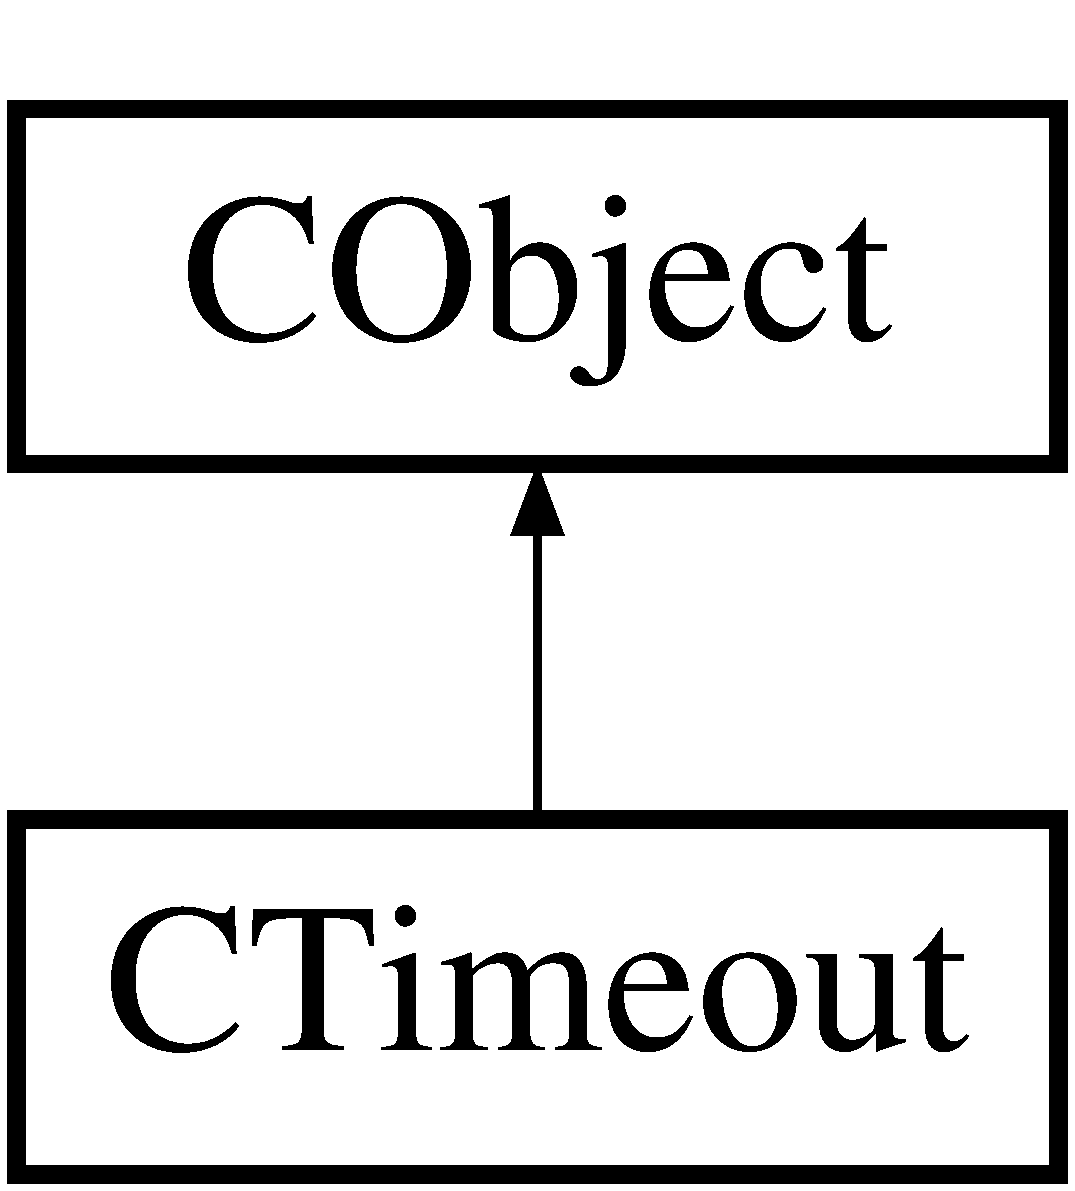
\includegraphics[height=2.000000cm]{d5/d5b/class_c_timeout}
\end{center}
\end{figure}
\subsection*{Public Member Functions}
\begin{DoxyCompactItemize}
\item 
\hyperlink{class_c_timeout_ac01d1f8a0d214687ff63cd6d915729de}{C\-Timeout} ()
\item 
virtual void \hyperlink{class_c_timeout_a663a09bb51c1de8f8d83bd62fdc1a688}{reset} ()
\item 
virtual void \hyperlink{class_c_timeout_a05315e59fa44ceafe8c9e444af0ac9e8}{wait} (int ms)
\item 
virtual void \hyperlink{class_c_timeout_ab2edd08150efbd3ef36766c7e02f7792}{wait} (float sec)
\item 
virtual uint32\-\_\-t \hyperlink{class_c_timeout_a1858ddcad4e18f8056441072616a457f}{elapsed} ()
\item 
virtual bool \hyperlink{class_c_timeout_a3841c7c53689d2ef8559a6c5e402aa5b}{is\-Expired} (uint32\-\_\-t to)
\item 
virtual float \hyperlink{class_c_timeout_a8af3a09c9ed9172b37e930d05865cfac}{read} ()
\end{DoxyCompactItemize}
\subsection*{Protected Attributes}
\begin{DoxyCompactItemize}
\item 
uint32\-\_\-t \hyperlink{class_c_timeout_a70d74daffca8e29ae4682dae45bb9f8f}{m\-\_\-tick}
\end{DoxyCompactItemize}


\subsection{Constructor \& Destructor Documentation}
\hypertarget{class_c_timeout_ac01d1f8a0d214687ff63cd6d915729de}{\index{C\-Timeout@{C\-Timeout}!C\-Timeout@{C\-Timeout}}
\index{C\-Timeout@{C\-Timeout}!CTimeout@{C\-Timeout}}
\subsubsection[{C\-Timeout}]{\setlength{\rightskip}{0pt plus 5cm}C\-Timeout\-::\-C\-Timeout (
\begin{DoxyParamCaption}
{}
\end{DoxyParamCaption}
)}}\label{class_c_timeout_ac01d1f8a0d214687ff63cd6d915729de}


\subsection{Member Function Documentation}
\hypertarget{class_c_timeout_a663a09bb51c1de8f8d83bd62fdc1a688}{\index{C\-Timeout@{C\-Timeout}!reset@{reset}}
\index{reset@{reset}!CTimeout@{C\-Timeout}}
\subsubsection[{reset}]{\setlength{\rightskip}{0pt plus 5cm}virtual void C\-Timeout\-::reset (
\begin{DoxyParamCaption}
{}
\end{DoxyParamCaption}
)\hspace{0.3cm}{\ttfamily [virtual]}}}\label{class_c_timeout_a663a09bb51c1de8f8d83bd62fdc1a688}
\hypertarget{class_c_timeout_a05315e59fa44ceafe8c9e444af0ac9e8}{\index{C\-Timeout@{C\-Timeout}!wait@{wait}}
\index{wait@{wait}!CTimeout@{C\-Timeout}}
\subsubsection[{wait}]{\setlength{\rightskip}{0pt plus 5cm}virtual void C\-Timeout\-::wait (
\begin{DoxyParamCaption}
\item[{int}]{ms}
\end{DoxyParamCaption}
)\hspace{0.3cm}{\ttfamily [virtual]}}}\label{class_c_timeout_a05315e59fa44ceafe8c9e444af0ac9e8}
\hypertarget{class_c_timeout_ab2edd08150efbd3ef36766c7e02f7792}{\index{C\-Timeout@{C\-Timeout}!wait@{wait}}
\index{wait@{wait}!CTimeout@{C\-Timeout}}
\subsubsection[{wait}]{\setlength{\rightskip}{0pt plus 5cm}virtual void C\-Timeout\-::wait (
\begin{DoxyParamCaption}
\item[{float}]{sec}
\end{DoxyParamCaption}
)\hspace{0.3cm}{\ttfamily [inline]}, {\ttfamily [virtual]}}}\label{class_c_timeout_ab2edd08150efbd3ef36766c7e02f7792}
\hypertarget{class_c_timeout_a1858ddcad4e18f8056441072616a457f}{\index{C\-Timeout@{C\-Timeout}!elapsed@{elapsed}}
\index{elapsed@{elapsed}!CTimeout@{C\-Timeout}}
\subsubsection[{elapsed}]{\setlength{\rightskip}{0pt plus 5cm}virtual uint32\-\_\-t C\-Timeout\-::elapsed (
\begin{DoxyParamCaption}
{}
\end{DoxyParamCaption}
)\hspace{0.3cm}{\ttfamily [virtual]}}}\label{class_c_timeout_a1858ddcad4e18f8056441072616a457f}
\hypertarget{class_c_timeout_a3841c7c53689d2ef8559a6c5e402aa5b}{\index{C\-Timeout@{C\-Timeout}!is\-Expired@{is\-Expired}}
\index{is\-Expired@{is\-Expired}!CTimeout@{C\-Timeout}}
\subsubsection[{is\-Expired}]{\setlength{\rightskip}{0pt plus 5cm}virtual bool C\-Timeout\-::is\-Expired (
\begin{DoxyParamCaption}
\item[{uint32\-\_\-t}]{to}
\end{DoxyParamCaption}
)\hspace{0.3cm}{\ttfamily [inline]}, {\ttfamily [virtual]}}}\label{class_c_timeout_a3841c7c53689d2ef8559a6c5e402aa5b}
\hypertarget{class_c_timeout_a8af3a09c9ed9172b37e930d05865cfac}{\index{C\-Timeout@{C\-Timeout}!read@{read}}
\index{read@{read}!CTimeout@{C\-Timeout}}
\subsubsection[{read}]{\setlength{\rightskip}{0pt plus 5cm}virtual float C\-Timeout\-::read (
\begin{DoxyParamCaption}
{}
\end{DoxyParamCaption}
)\hspace{0.3cm}{\ttfamily [inline]}, {\ttfamily [virtual]}}}\label{class_c_timeout_a8af3a09c9ed9172b37e930d05865cfac}
Reterive timeout value \begin{DoxyReturn}{Returns}
float second 
\end{DoxyReturn}


\subsection{Member Data Documentation}
\hypertarget{class_c_timeout_a70d74daffca8e29ae4682dae45bb9f8f}{\index{C\-Timeout@{C\-Timeout}!m\-\_\-tick@{m\-\_\-tick}}
\index{m\-\_\-tick@{m\-\_\-tick}!CTimeout@{C\-Timeout}}
\subsubsection[{m\-\_\-tick}]{\setlength{\rightskip}{0pt plus 5cm}uint32\-\_\-t C\-Timeout\-::m\-\_\-tick\hspace{0.3cm}{\ttfamily [protected]}}}\label{class_c_timeout_a70d74daffca8e29ae4682dae45bb9f8f}


The documentation for this class was generated from the following file\-:\begin{DoxyCompactItemize}
\item 
timeout.\-h\end{DoxyCompactItemize}

\hypertarget{class_c_timer}{\section{C\-Timer Class Reference}
\label{class_c_timer}\index{C\-Timer@{C\-Timer}}
}
Inheritance diagram for C\-Timer\-:\begin{figure}[H]
\begin{center}
\leavevmode
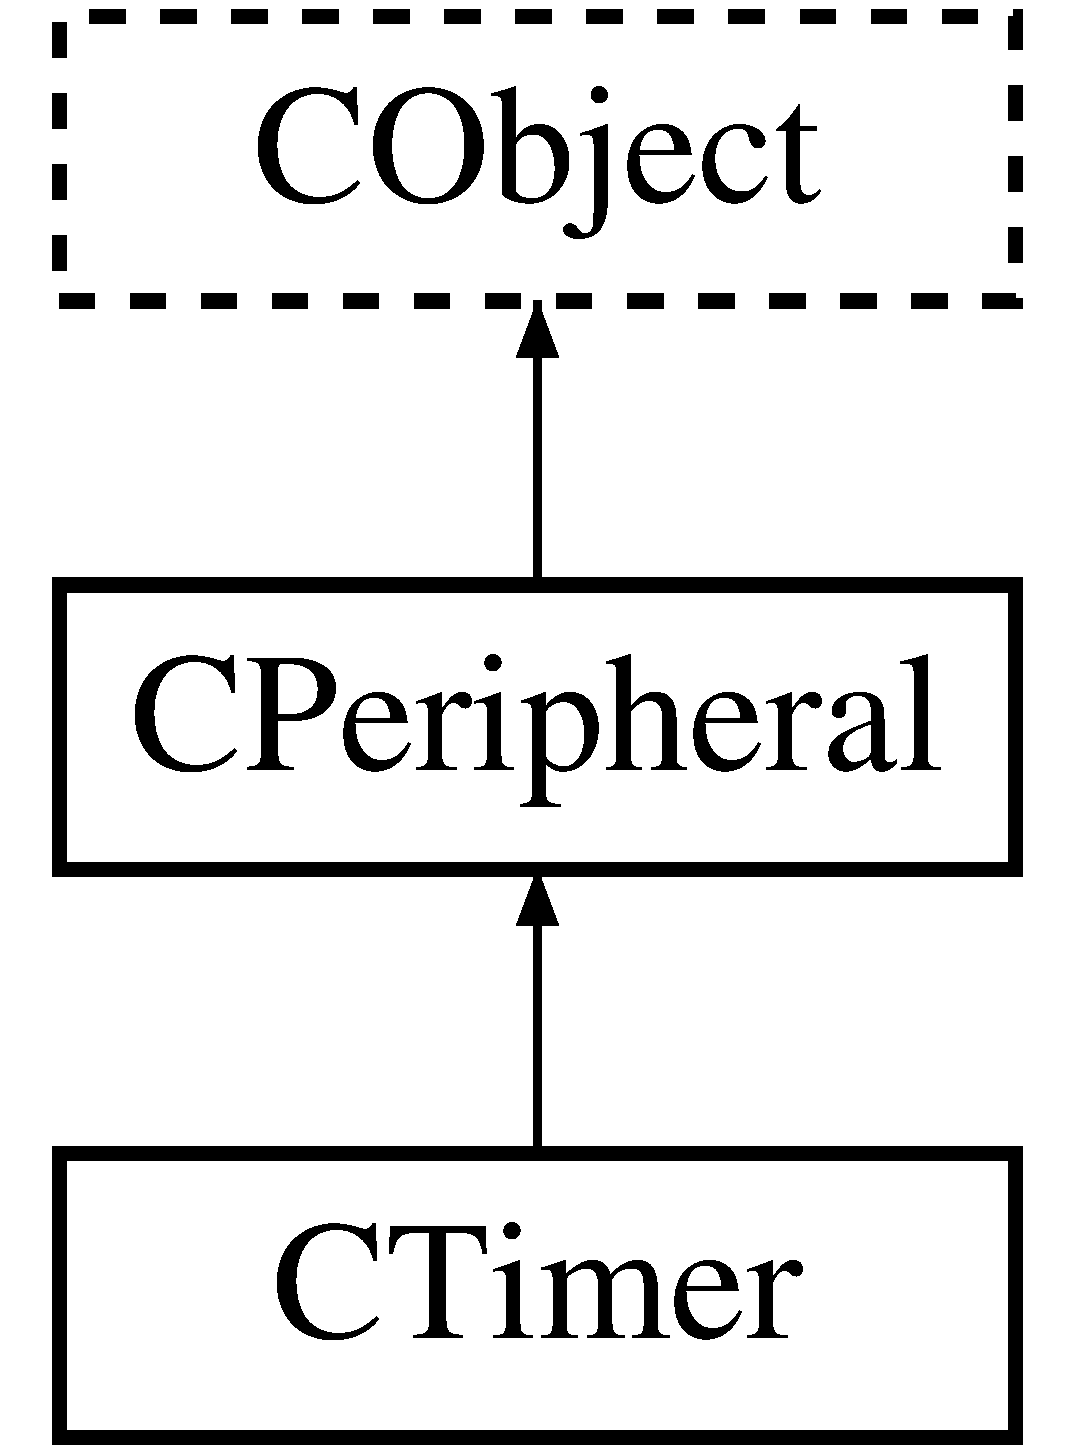
\includegraphics[height=3.000000cm]{class_c_timer}
\end{center}
\end{figure}
\subsection*{Public Member Functions}
\begin{DoxyCompactItemize}
\item 
\hypertarget{class_c_timer_a01988907cb23d887bf9db237ecac1d8f}{{\bfseries C\-Timer} (T\-I\-M\-E\-R\-\_\-\-T t)}\label{class_c_timer_a01988907cb23d887bf9db237ecac1d8f}

\item 
\hypertarget{class_c_timer_aa4d48f568d057eccc1842748034fadbf}{void {\bfseries second} (float sec)}\label{class_c_timer_aa4d48f568d057eccc1842748034fadbf}

\item 
\hypertarget{class_c_timer_a80328fea91b61d9ffb154671b5cae6df}{void {\bfseries millisecond} (uint32\-\_\-t ms)}\label{class_c_timer_a80328fea91b61d9ffb154671b5cae6df}

\item 
\hypertarget{class_c_timer_aeffc80e8f34a8c1e5e0850da92b7ee17}{void {\bfseries enable} ()}\label{class_c_timer_aeffc80e8f34a8c1e5e0850da92b7ee17}

\item 
\hypertarget{class_c_timer_a61c79a568b4337520ed58e5f248a068e}{void {\bfseries disable} ()}\label{class_c_timer_a61c79a568b4337520ed58e5f248a068e}

\item 
\hypertarget{class_c_timer_ab94e07fab4cea184d1b02de1c9435b02}{void {\bfseries begin} ()}\label{class_c_timer_ab94e07fab4cea184d1b02de1c9435b02}

\item 
\hypertarget{class_c_timer_a7258888c2b3954fa3922201595e562a8}{void {\bfseries end} ()}\label{class_c_timer_a7258888c2b3954fa3922201595e562a8}

\item 
\hypertarget{class_c_timer_a6234aac53e301116247e33254cd2f585}{void {\bfseries reset} ()}\label{class_c_timer_a6234aac53e301116247e33254cd2f585}

\item 
\hypertarget{class_c_timer_a9e63f073da87bd67b2afded332d2aa2d}{bool {\bfseries wait} (uint32\-\_\-t timeout=M\-A\-X\-\_\-\-D\-E\-L\-A\-Y\-\_\-\-T\-I\-M\-E)}\label{class_c_timer_a9e63f073da87bd67b2afded332d2aa2d}

\item 
\hypertarget{class_c_timer_a54ec6171b2f4f7af4fd5f3b43a486d02}{uint32\-\_\-t {\bfseries count} ()}\label{class_c_timer_a54ec6171b2f4f7af4fd5f3b43a486d02}

\end{DoxyCompactItemize}
\subsection*{Static Public Member Functions}
\begin{DoxyCompactItemize}
\item 
\hypertarget{class_c_timer_a2021fd4d79d43498822c376625dd511b}{static T\-I\-M\-E\-R\-\_\-\-T {\bfseries get\-Unused} ()}\label{class_c_timer_a2021fd4d79d43498822c376625dd511b}

\end{DoxyCompactItemize}
\subsection*{Public Attributes}
\begin{DoxyCompactItemize}
\item 
\hypertarget{class_c_timer_a1bd7d3dbb8bfeeb5e603a7f7c0eed5c7}{\hyperlink{class_c_semaphore}{C\-Semaphore} {\bfseries m\-\_\-sem\-Irq}}\label{class_c_timer_a1bd7d3dbb8bfeeb5e603a7f7c0eed5c7}

\item 
\hypertarget{class_c_timer_a0ab331eadfa7223dfe9344db39dac615}{uint32\-\_\-t {\bfseries m\-\_\-count}}\label{class_c_timer_a0ab331eadfa7223dfe9344db39dac615}

\end{DoxyCompactItemize}


The documentation for this class was generated from the following file\-:\begin{DoxyCompactItemize}
\item 
timer.\-h\end{DoxyCompactItemize}

\hypertarget{class_c_watchdog}{\section{C\-Watchdog Class Reference}
\label{class_c_watchdog}\index{C\-Watchdog@{C\-Watchdog}}
}


{\ttfamily \#include $<$watchdog.\-h$>$}

Inheritance diagram for C\-Watchdog\-:\begin{figure}[H]
\begin{center}
\leavevmode
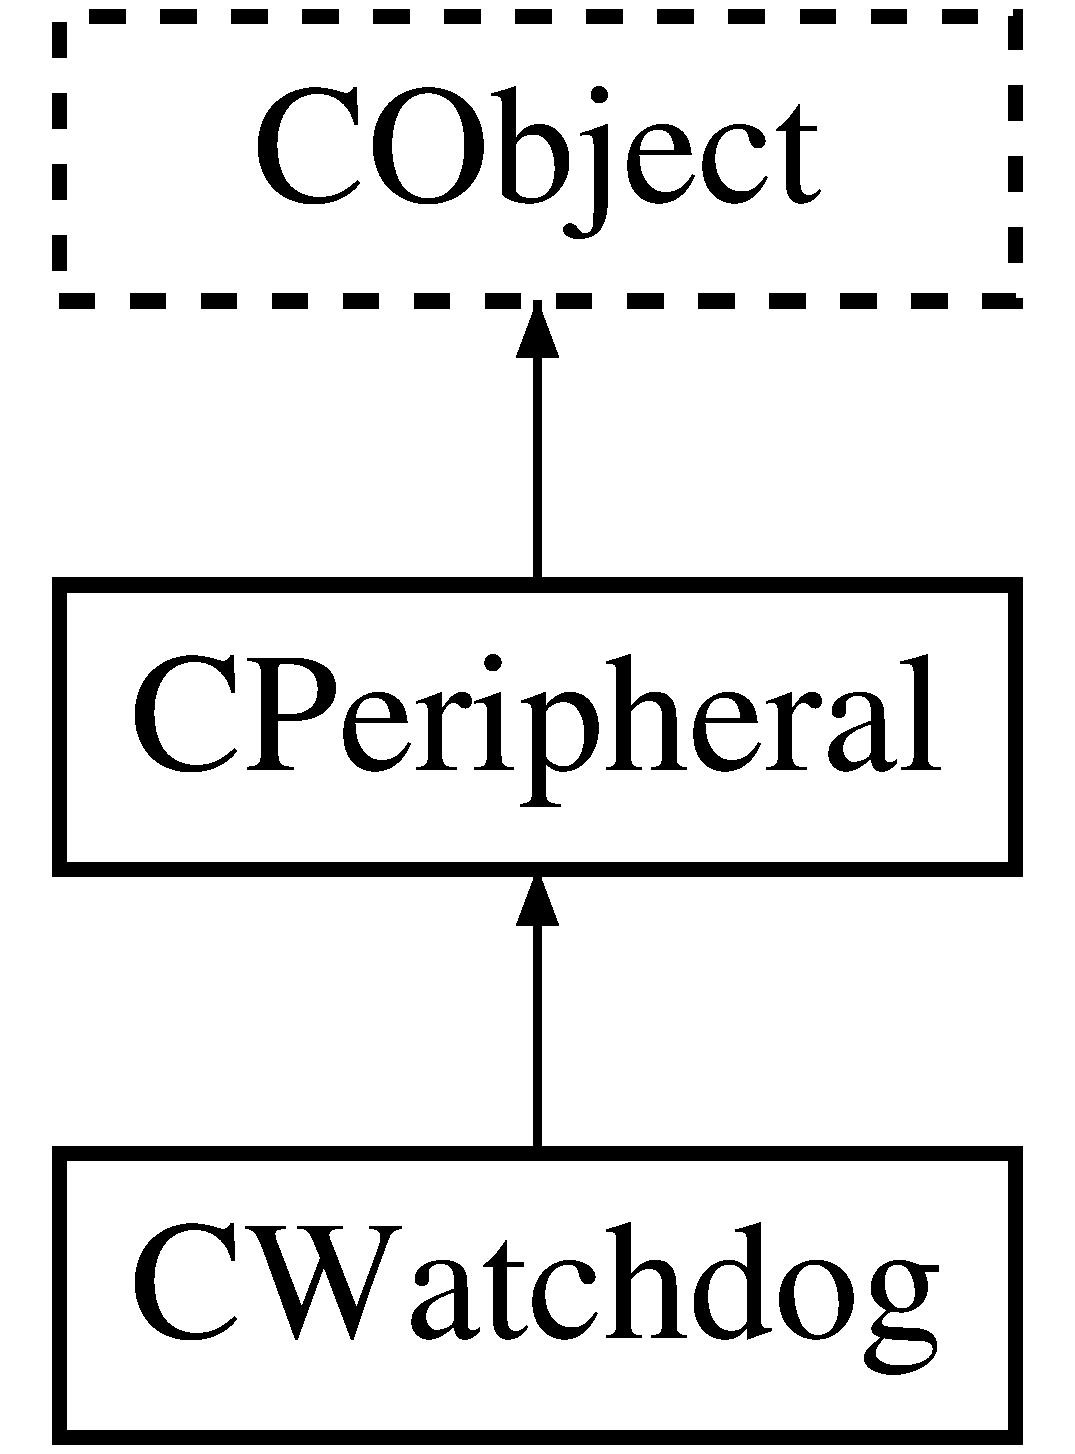
\includegraphics[height=3.000000cm]{d3/d75/class_c_watchdog}
\end{center}
\end{figure}
\subsection*{Public Member Functions}
\begin{DoxyCompactItemize}
\item 
\hyperlink{class_c_watchdog_ab2859bc21e221a86d73e1dc3877b8f86}{C\-Watchdog} ()
\item 
void \hyperlink{class_c_watchdog_af9dc7eb09403e54c36ffce01e1932f1e}{set\-Timeout} (float second)
\item 
void \hyperlink{class_c_watchdog_afbc1961aa586367e2bfaf36388bdbccb}{enable} (float warming)
\item 
void \hyperlink{class_c_watchdog_a7b59eeaca4965e03559e327131d76979}{disable} ()
\item 
virtual bool \hyperlink{class_c_watchdog_a252da476793090998b1086c99bbbd1ab}{wait} (uint32\-\_\-t timeout=M\-A\-X\-\_\-\-D\-E\-L\-A\-Y\-\_\-\-T\-I\-M\-E)
\item 
void \hyperlink{class_c_watchdog_ae0b02e76a4c9e853aec3d5526dd33963}{as\-Wakeup\-Source} ()
\item 
uint32\-\_\-t \hyperlink{class_c_watchdog_ac6c20aa855ac46780e63de1f745c4d6b}{count} ()
\item 
virtual \hyperlink{class_c_watchdog_a95284e312f91b18f52eacd6e6daeacaf}{$\sim$\-C\-Watchdog} ()
\end{DoxyCompactItemize}
\subsection*{Static Public Member Functions}
\begin{DoxyCompactItemize}
\item 
static void \hyperlink{class_c_watchdog_a34f816a6e2a53dc92943e9c309244130}{feed} ()
\item 
static uint32\-\_\-t \hyperlink{class_c_watchdog_a231300cd97144342d7d3d9606cb9b60c}{frequence} ()
\end{DoxyCompactItemize}
\subsection*{Public Attributes}
\begin{DoxyCompactItemize}
\item 
\hyperlink{class_c_semaphore}{C\-Semaphore} \hyperlink{class_c_watchdog_afac017788a234968c352f037ebb77649}{m\-\_\-sem\-Irq}
\end{DoxyCompactItemize}


\subsection{Constructor \& Destructor Documentation}
\hypertarget{class_c_watchdog_ab2859bc21e221a86d73e1dc3877b8f86}{\index{C\-Watchdog@{C\-Watchdog}!C\-Watchdog@{C\-Watchdog}}
\index{C\-Watchdog@{C\-Watchdog}!CWatchdog@{C\-Watchdog}}
\subsubsection[{C\-Watchdog}]{\setlength{\rightskip}{0pt plus 5cm}C\-Watchdog\-::\-C\-Watchdog (
\begin{DoxyParamCaption}
{}
\end{DoxyParamCaption}
)}}\label{class_c_watchdog_ab2859bc21e221a86d73e1dc3877b8f86}
\hypertarget{class_c_watchdog_a95284e312f91b18f52eacd6e6daeacaf}{\index{C\-Watchdog@{C\-Watchdog}!$\sim$\-C\-Watchdog@{$\sim$\-C\-Watchdog}}
\index{$\sim$\-C\-Watchdog@{$\sim$\-C\-Watchdog}!CWatchdog@{C\-Watchdog}}
\subsubsection[{$\sim$\-C\-Watchdog}]{\setlength{\rightskip}{0pt plus 5cm}virtual C\-Watchdog\-::$\sim$\-C\-Watchdog (
\begin{DoxyParamCaption}
{}
\end{DoxyParamCaption}
)\hspace{0.3cm}{\ttfamily [virtual]}}}\label{class_c_watchdog_a95284e312f91b18f52eacd6e6daeacaf}


\subsection{Member Function Documentation}
\hypertarget{class_c_watchdog_af9dc7eb09403e54c36ffce01e1932f1e}{\index{C\-Watchdog@{C\-Watchdog}!set\-Timeout@{set\-Timeout}}
\index{set\-Timeout@{set\-Timeout}!CWatchdog@{C\-Watchdog}}
\subsubsection[{set\-Timeout}]{\setlength{\rightskip}{0pt plus 5cm}void C\-Watchdog\-::set\-Timeout (
\begin{DoxyParamCaption}
\item[{float}]{second}
\end{DoxyParamCaption}
)}}\label{class_c_watchdog_af9dc7eb09403e54c36ffce01e1932f1e}
\hypertarget{class_c_watchdog_afbc1961aa586367e2bfaf36388bdbccb}{\index{C\-Watchdog@{C\-Watchdog}!enable@{enable}}
\index{enable@{enable}!CWatchdog@{C\-Watchdog}}
\subsubsection[{enable}]{\setlength{\rightskip}{0pt plus 5cm}void C\-Watchdog\-::enable (
\begin{DoxyParamCaption}
\item[{float}]{warming}
\end{DoxyParamCaption}
)}}\label{class_c_watchdog_afbc1961aa586367e2bfaf36388bdbccb}
\hypertarget{class_c_watchdog_a7b59eeaca4965e03559e327131d76979}{\index{C\-Watchdog@{C\-Watchdog}!disable@{disable}}
\index{disable@{disable}!CWatchdog@{C\-Watchdog}}
\subsubsection[{disable}]{\setlength{\rightskip}{0pt plus 5cm}void C\-Watchdog\-::disable (
\begin{DoxyParamCaption}
{}
\end{DoxyParamCaption}
)}}\label{class_c_watchdog_a7b59eeaca4965e03559e327131d76979}
\hypertarget{class_c_watchdog_a34f816a6e2a53dc92943e9c309244130}{\index{C\-Watchdog@{C\-Watchdog}!feed@{feed}}
\index{feed@{feed}!CWatchdog@{C\-Watchdog}}
\subsubsection[{feed}]{\setlength{\rightskip}{0pt plus 5cm}static void C\-Watchdog\-::feed (
\begin{DoxyParamCaption}
{}
\end{DoxyParamCaption}
)\hspace{0.3cm}{\ttfamily [static]}}}\label{class_c_watchdog_a34f816a6e2a53dc92943e9c309244130}
\hypertarget{class_c_watchdog_a231300cd97144342d7d3d9606cb9b60c}{\index{C\-Watchdog@{C\-Watchdog}!frequence@{frequence}}
\index{frequence@{frequence}!CWatchdog@{C\-Watchdog}}
\subsubsection[{frequence}]{\setlength{\rightskip}{0pt plus 5cm}static uint32\-\_\-t C\-Watchdog\-::frequence (
\begin{DoxyParamCaption}
{}
\end{DoxyParamCaption}
)\hspace{0.3cm}{\ttfamily [static]}}}\label{class_c_watchdog_a231300cd97144342d7d3d9606cb9b60c}
\hypertarget{class_c_watchdog_a252da476793090998b1086c99bbbd1ab}{\index{C\-Watchdog@{C\-Watchdog}!wait@{wait}}
\index{wait@{wait}!CWatchdog@{C\-Watchdog}}
\subsubsection[{wait}]{\setlength{\rightskip}{0pt plus 5cm}virtual bool C\-Watchdog\-::wait (
\begin{DoxyParamCaption}
\item[{uint32\-\_\-t}]{timeout = {\ttfamily MAX\-\_\-DELAY\-\_\-TIME}}
\end{DoxyParamCaption}
)\hspace{0.3cm}{\ttfamily [virtual]}}}\label{class_c_watchdog_a252da476793090998b1086c99bbbd1ab}
\hypertarget{class_c_watchdog_ae0b02e76a4c9e853aec3d5526dd33963}{\index{C\-Watchdog@{C\-Watchdog}!as\-Wakeup\-Source@{as\-Wakeup\-Source}}
\index{as\-Wakeup\-Source@{as\-Wakeup\-Source}!CWatchdog@{C\-Watchdog}}
\subsubsection[{as\-Wakeup\-Source}]{\setlength{\rightskip}{0pt plus 5cm}void C\-Watchdog\-::as\-Wakeup\-Source (
\begin{DoxyParamCaption}
{}
\end{DoxyParamCaption}
)}}\label{class_c_watchdog_ae0b02e76a4c9e853aec3d5526dd33963}
\hypertarget{class_c_watchdog_ac6c20aa855ac46780e63de1f745c4d6b}{\index{C\-Watchdog@{C\-Watchdog}!count@{count}}
\index{count@{count}!CWatchdog@{C\-Watchdog}}
\subsubsection[{count}]{\setlength{\rightskip}{0pt plus 5cm}uint32\-\_\-t C\-Watchdog\-::count (
\begin{DoxyParamCaption}
{}
\end{DoxyParamCaption}
)}}\label{class_c_watchdog_ac6c20aa855ac46780e63de1f745c4d6b}


\subsection{Member Data Documentation}
\hypertarget{class_c_watchdog_afac017788a234968c352f037ebb77649}{\index{C\-Watchdog@{C\-Watchdog}!m\-\_\-sem\-Irq@{m\-\_\-sem\-Irq}}
\index{m\-\_\-sem\-Irq@{m\-\_\-sem\-Irq}!CWatchdog@{C\-Watchdog}}
\subsubsection[{m\-\_\-sem\-Irq}]{\setlength{\rightskip}{0pt plus 5cm}{\bf C\-Semaphore} C\-Watchdog\-::m\-\_\-sem\-Irq}}\label{class_c_watchdog_afac017788a234968c352f037ebb77649}


The documentation for this class was generated from the following file\-:\begin{DoxyCompactItemize}
\item 
watchdog.\-h\end{DoxyCompactItemize}

\hypertarget{class_e_e_p_r_o_m}{\section{E\-E\-P\-R\-O\-M Class Reference}
\label{class_e_e_p_r_o_m}\index{E\-E\-P\-R\-O\-M@{E\-E\-P\-R\-O\-M}}
}


{\ttfamily \#include $<$eeprom.\-h$>$}

Inheritance diagram for E\-E\-P\-R\-O\-M\-:\begin{figure}[H]
\begin{center}
\leavevmode
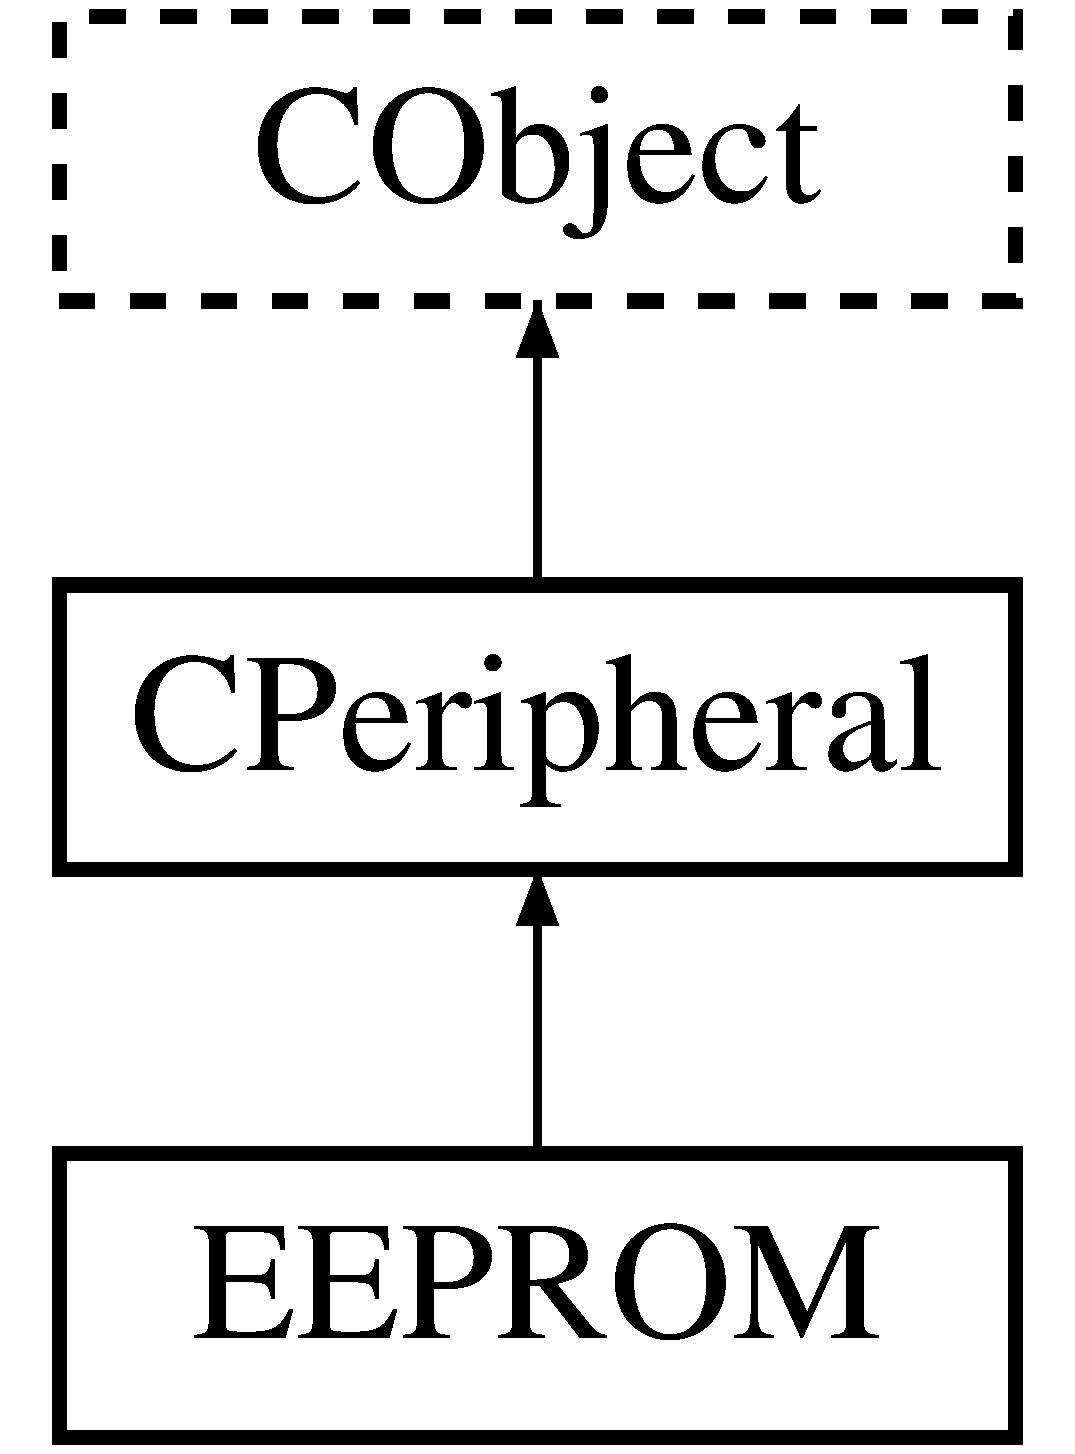
\includegraphics[height=3.000000cm]{d0/d7a/class_e_e_p_r_o_m}
\end{center}
\end{figure}
\subsection*{Static Public Member Functions}
\begin{DoxyCompactItemize}
\item 
static bool \hyperlink{class_e_e_p_r_o_m_a47f3f52eed97b6e43b830ce4a1dc495e}{read} (unsigned addr, void $\ast$buf, unsigned size)
\item 
static bool \hyperlink{class_e_e_p_r_o_m_a8c397be98d4762869715a2a07866af6b}{write} (unsigned addr, void $\ast$buf, unsigned size)
\end{DoxyCompactItemize}
\subsection*{Additional Inherited Members}


\subsection{Member Function Documentation}
\hypertarget{class_e_e_p_r_o_m_a47f3f52eed97b6e43b830ce4a1dc495e}{\index{E\-E\-P\-R\-O\-M@{E\-E\-P\-R\-O\-M}!read@{read}}
\index{read@{read}!EEPROM@{E\-E\-P\-R\-O\-M}}
\subsubsection[{read}]{\setlength{\rightskip}{0pt plus 5cm}static bool E\-E\-P\-R\-O\-M\-::read (
\begin{DoxyParamCaption}
\item[{unsigned}]{addr, }
\item[{void $\ast$}]{buf, }
\item[{unsigned}]{size}
\end{DoxyParamCaption}
)\hspace{0.3cm}{\ttfamily [static]}}}\label{class_e_e_p_r_o_m_a47f3f52eed97b6e43b830ce4a1dc495e}
\hypertarget{class_e_e_p_r_o_m_a8c397be98d4762869715a2a07866af6b}{\index{E\-E\-P\-R\-O\-M@{E\-E\-P\-R\-O\-M}!write@{write}}
\index{write@{write}!EEPROM@{E\-E\-P\-R\-O\-M}}
\subsubsection[{write}]{\setlength{\rightskip}{0pt plus 5cm}static bool E\-E\-P\-R\-O\-M\-::write (
\begin{DoxyParamCaption}
\item[{unsigned}]{addr, }
\item[{void $\ast$}]{buf, }
\item[{unsigned}]{size}
\end{DoxyParamCaption}
)\hspace{0.3cm}{\ttfamily [static]}}}\label{class_e_e_p_r_o_m_a8c397be98d4762869715a2a07866af6b}


The documentation for this class was generated from the following file\-:\begin{DoxyCompactItemize}
\item 
eeprom.\-h\end{DoxyCompactItemize}

\hypertarget{structfifo__t}{\section{fifo\-\_\-t Struct Reference}
\label{structfifo__t}\index{fifo\-\_\-t@{fifo\-\_\-t}}
}


{\ttfamily \#include $<$fifo.\-h$>$}

\subsection*{Public Attributes}
\begin{DoxyCompactItemize}
\item 
int \hyperlink{structfifo__t_adfe58cd24e80a0d62cf830bcc83f5c01}{size}
\item 
int \hyperlink{structfifo__t_ae93028e986799fceacecbd153729f855}{head}
\item 
int \hyperlink{structfifo__t_abe914ae9dd92644d8a53a4b99d89b487}{tail}
\item 
uint8\-\_\-t $\ast$ \hyperlink{structfifo__t_a6179dabda649717df17b5a38dbf0d744}{buf}
\end{DoxyCompactItemize}


\subsection{Member Data Documentation}
\hypertarget{structfifo__t_adfe58cd24e80a0d62cf830bcc83f5c01}{\index{fifo\-\_\-t@{fifo\-\_\-t}!size@{size}}
\index{size@{size}!fifo_t@{fifo\-\_\-t}}
\subsubsection[{size}]{\setlength{\rightskip}{0pt plus 5cm}int fifo\-\_\-t\-::size}}\label{structfifo__t_adfe58cd24e80a0d62cf830bcc83f5c01}
\hypertarget{structfifo__t_ae93028e986799fceacecbd153729f855}{\index{fifo\-\_\-t@{fifo\-\_\-t}!head@{head}}
\index{head@{head}!fifo_t@{fifo\-\_\-t}}
\subsubsection[{head}]{\setlength{\rightskip}{0pt plus 5cm}int fifo\-\_\-t\-::head}}\label{structfifo__t_ae93028e986799fceacecbd153729f855}
\hypertarget{structfifo__t_abe914ae9dd92644d8a53a4b99d89b487}{\index{fifo\-\_\-t@{fifo\-\_\-t}!tail@{tail}}
\index{tail@{tail}!fifo_t@{fifo\-\_\-t}}
\subsubsection[{tail}]{\setlength{\rightskip}{0pt plus 5cm}int fifo\-\_\-t\-::tail}}\label{structfifo__t_abe914ae9dd92644d8a53a4b99d89b487}
\hypertarget{structfifo__t_a6179dabda649717df17b5a38dbf0d744}{\index{fifo\-\_\-t@{fifo\-\_\-t}!buf@{buf}}
\index{buf@{buf}!fifo_t@{fifo\-\_\-t}}
\subsubsection[{buf}]{\setlength{\rightskip}{0pt plus 5cm}uint8\-\_\-t$\ast$ fifo\-\_\-t\-::buf}}\label{structfifo__t_a6179dabda649717df17b5a38dbf0d744}


The documentation for this struct was generated from the following file\-:\begin{DoxyCompactItemize}
\item 
fifo.\-h\end{DoxyCompactItemize}

\hypertarget{structble_health_thermometer_1_1h__thermo__temp__measure__t}{\section{ble\-Health\-Thermometer\-:\-:h\-\_\-thermo\-\_\-temp\-\_\-measure\-\_\-t Struct Reference}
\label{structble_health_thermometer_1_1h__thermo__temp__measure__t}\index{ble\-Health\-Thermometer\-::h\-\_\-thermo\-\_\-temp\-\_\-measure\-\_\-t@{ble\-Health\-Thermometer\-::h\-\_\-thermo\-\_\-temp\-\_\-measure\-\_\-t}}
}


{\ttfamily \#include $<$ble\-\_\-ht.\-h$>$}

\subsection*{Public Attributes}
\begin{DoxyCompactItemize}
\item 
uint8\-\_\-t \hyperlink{structble_health_thermometer_1_1h__thermo__temp__measure__t_ad2beee2a9d16609e0171df720eea4fc4}{flags}
\item 
uint8\-\_\-t \hyperlink{structble_health_thermometer_1_1h__thermo__temp__measure__t_ae65911e1474d1271d982d70b2624609f}{measurement} \mbox{[}4\mbox{]}
\item 
uint8\-\_\-t \hyperlink{structble_health_thermometer_1_1h__thermo__temp__measure__t_a5827f7c41051575943c0b7c85a20ef72}{time\-\_\-type} \mbox{[}8\mbox{]}
\end{DoxyCompactItemize}


\subsection{Detailed Description}
Temperature measurement structure 

\subsection{Member Data Documentation}
\hypertarget{structble_health_thermometer_1_1h__thermo__temp__measure__t_ad2beee2a9d16609e0171df720eea4fc4}{\index{ble\-Health\-Thermometer\-::h\-\_\-thermo\-\_\-temp\-\_\-measure\-\_\-t@{ble\-Health\-Thermometer\-::h\-\_\-thermo\-\_\-temp\-\_\-measure\-\_\-t}!flags@{flags}}
\index{flags@{flags}!bleHealthThermometer::h_thermo_temp_measure_t@{ble\-Health\-Thermometer\-::h\-\_\-thermo\-\_\-temp\-\_\-measure\-\_\-t}}
\subsubsection[{flags}]{\setlength{\rightskip}{0pt plus 5cm}uint8\-\_\-t ble\-Health\-Thermometer\-::h\-\_\-thermo\-\_\-temp\-\_\-measure\-\_\-t\-::flags}}\label{structble_health_thermometer_1_1h__thermo__temp__measure__t_ad2beee2a9d16609e0171df720eea4fc4}
\hypertarget{structble_health_thermometer_1_1h__thermo__temp__measure__t_ae65911e1474d1271d982d70b2624609f}{\index{ble\-Health\-Thermometer\-::h\-\_\-thermo\-\_\-temp\-\_\-measure\-\_\-t@{ble\-Health\-Thermometer\-::h\-\_\-thermo\-\_\-temp\-\_\-measure\-\_\-t}!measurement@{measurement}}
\index{measurement@{measurement}!bleHealthThermometer::h_thermo_temp_measure_t@{ble\-Health\-Thermometer\-::h\-\_\-thermo\-\_\-temp\-\_\-measure\-\_\-t}}
\subsubsection[{measurement}]{\setlength{\rightskip}{0pt plus 5cm}uint8\-\_\-t ble\-Health\-Thermometer\-::h\-\_\-thermo\-\_\-temp\-\_\-measure\-\_\-t\-::measurement\mbox{[}4\mbox{]}}}\label{structble_health_thermometer_1_1h__thermo__temp__measure__t_ae65911e1474d1271d982d70b2624609f}
\hypertarget{structble_health_thermometer_1_1h__thermo__temp__measure__t_a5827f7c41051575943c0b7c85a20ef72}{\index{ble\-Health\-Thermometer\-::h\-\_\-thermo\-\_\-temp\-\_\-measure\-\_\-t@{ble\-Health\-Thermometer\-::h\-\_\-thermo\-\_\-temp\-\_\-measure\-\_\-t}!time\-\_\-type@{time\-\_\-type}}
\index{time\-\_\-type@{time\-\_\-type}!bleHealthThermometer::h_thermo_temp_measure_t@{ble\-Health\-Thermometer\-::h\-\_\-thermo\-\_\-temp\-\_\-measure\-\_\-t}}
\subsubsection[{time\-\_\-type}]{\setlength{\rightskip}{0pt plus 5cm}uint8\-\_\-t ble\-Health\-Thermometer\-::h\-\_\-thermo\-\_\-temp\-\_\-measure\-\_\-t\-::time\-\_\-type\mbox{[}8\mbox{]}}}\label{structble_health_thermometer_1_1h__thermo__temp__measure__t_a5827f7c41051575943c0b7c85a20ef72}


The documentation for this struct was generated from the following file\-:\begin{DoxyCompactItemize}
\item 
ble\-\_\-ht.\-h\end{DoxyCompactItemize}

\hypertarget{union_i_p___a_d_d_r___t}{\section{I\-P\-\_\-\-A\-D\-D\-R\-\_\-\-T Union Reference}
\label{union_i_p___a_d_d_r___t}\index{I\-P\-\_\-\-A\-D\-D\-R\-\_\-\-T@{I\-P\-\_\-\-A\-D\-D\-R\-\_\-\-T}}
}
\subsection*{Public Attributes}
\begin{DoxyCompactItemize}
\item 
\hypertarget{union_i_p___a_d_d_r___t_a7d804478df76fbcabec9ea3e252b07d4}{uint32\-\_\-t \hyperlink{union_i_p___a_d_d_r___t_a7d804478df76fbcabec9ea3e252b07d4}{addr}}\label{union_i_p___a_d_d_r___t_a7d804478df76fbcabec9ea3e252b07d4}

\begin{DoxyCompactList}\small\item\em a 32bits unsigned long integer type address \end{DoxyCompactList}\item 
\hypertarget{union_i_p___a_d_d_r___t_a46438b841f54b90fdaa0ef824dbcc2c2}{uint8\-\_\-t \hyperlink{union_i_p___a_d_d_r___t_a46438b841f54b90fdaa0ef824dbcc2c2}{addr8} \mbox{[}4\mbox{]}}\label{union_i_p___a_d_d_r___t_a46438b841f54b90fdaa0ef824dbcc2c2}

\begin{DoxyCompactList}\small\item\em a 4 bytes array address \end{DoxyCompactList}\end{DoxyCompactItemize}


The documentation for this union was generated from the following file\-:\begin{DoxyCompactItemize}
\item 
u\-C\-Xpresso.\-h\end{DoxyCompactItemize}

\hypertarget{struct_s_y_s___i_d___t}{\section{S\-Y\-S\-\_\-\-I\-D\-\_\-\-T Struct Reference}
\label{struct_s_y_s___i_d___t}\index{S\-Y\-S\-\_\-\-I\-D\-\_\-\-T@{S\-Y\-S\-\_\-\-I\-D\-\_\-\-T}}
}


{\ttfamily \#include $<$ble\-\_\-devinfo.\-h$>$}

\subsection*{Public Attributes}
\begin{DoxyCompactItemize}
\item 
uint8\-\_\-t \hyperlink{struct_s_y_s___i_d___t_a36a75b1bc4c8e4866eb039880b8aad9e}{mfg\-Id} \mbox{[}5\mbox{]}
\begin{DoxyCompactList}\small\item\em Manufacturer Identifier, 40 bits. \end{DoxyCompactList}\item 
uint8\-\_\-t \hyperlink{struct_s_y_s___i_d___t_aaf2c14195d90ec1c9de9b6c57c4fcd94}{org\-Id} \mbox{[}3\mbox{]}
\begin{DoxyCompactList}\small\item\em Organizationally Unique Identifier, 24 bits;. \end{DoxyCompactList}\end{DoxyCompactItemize}


\subsection{Detailed Description}
System Id for Device Information (B\-L\-E). 

\subsection{Member Data Documentation}
\hypertarget{struct_s_y_s___i_d___t_a36a75b1bc4c8e4866eb039880b8aad9e}{\index{S\-Y\-S\-\_\-\-I\-D\-\_\-\-T@{S\-Y\-S\-\_\-\-I\-D\-\_\-\-T}!mfg\-Id@{mfg\-Id}}
\index{mfg\-Id@{mfg\-Id}!SYS_ID_T@{S\-Y\-S\-\_\-\-I\-D\-\_\-\-T}}
\subsubsection[{mfg\-Id}]{\setlength{\rightskip}{0pt plus 5cm}uint8\-\_\-t S\-Y\-S\-\_\-\-I\-D\-\_\-\-T\-::mfg\-Id\mbox{[}5\mbox{]}}}\label{struct_s_y_s___i_d___t_a36a75b1bc4c8e4866eb039880b8aad9e}


Manufacturer Identifier, 40 bits. 

\hypertarget{struct_s_y_s___i_d___t_aaf2c14195d90ec1c9de9b6c57c4fcd94}{\index{S\-Y\-S\-\_\-\-I\-D\-\_\-\-T@{S\-Y\-S\-\_\-\-I\-D\-\_\-\-T}!org\-Id@{org\-Id}}
\index{org\-Id@{org\-Id}!SYS_ID_T@{S\-Y\-S\-\_\-\-I\-D\-\_\-\-T}}
\subsubsection[{org\-Id}]{\setlength{\rightskip}{0pt plus 5cm}uint8\-\_\-t S\-Y\-S\-\_\-\-I\-D\-\_\-\-T\-::org\-Id\mbox{[}3\mbox{]}}}\label{struct_s_y_s___i_d___t_aaf2c14195d90ec1c9de9b6c57c4fcd94}


Organizationally Unique Identifier, 24 bits;. 



The documentation for this struct was generated from the following file\-:\begin{DoxyCompactItemize}
\item 
ble\-\_\-devinfo.\-h\end{DoxyCompactItemize}

\hypertarget{classusb_c_d_c}{\section{usb\-C\-D\-C Class Reference}
\label{classusb_c_d_c}\index{usb\-C\-D\-C@{usb\-C\-D\-C}}
}
Inheritance diagram for usb\-C\-D\-C\-:\begin{figure}[H]
\begin{center}
\leavevmode
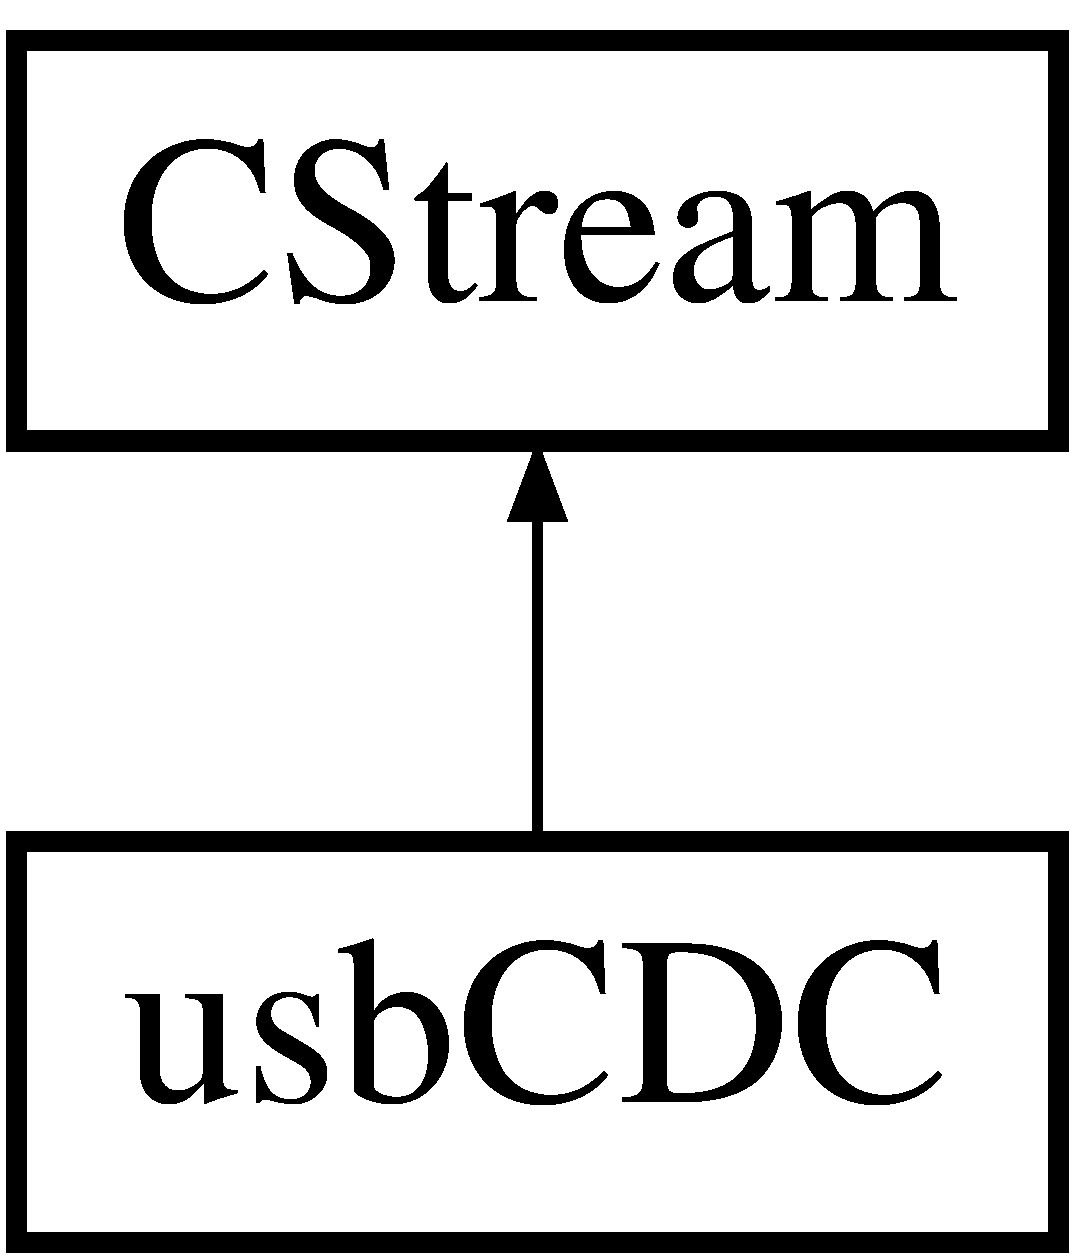
\includegraphics[height=2.000000cm]{classusb_c_d_c}
\end{center}
\end{figure}
\subsection*{Public Member Functions}
\begin{DoxyCompactItemize}
\item 
\hypertarget{classusb_c_d_c_a6eb4d9401ac17bab0bfb869bf6fc6315}{{\bfseries usb\-C\-D\-C} (int F\-I\-F\-O\-\_\-\-S\-I\-Z\-E=128)}\label{classusb_c_d_c_a6eb4d9401ac17bab0bfb869bf6fc6315}

\item 
\hypertarget{classusb_c_d_c_a49d431de50da7ccacf91ef33b04e99d2}{bool {\bfseries connect} ()}\label{classusb_c_d_c_a49d431de50da7ccacf91ef33b04e99d2}

\item 
\hypertarget{classusb_c_d_c_aa95f819926a8da40f12eebc62adf6f95}{bool {\bfseries disconnect} ()}\label{classusb_c_d_c_aa95f819926a8da40f12eebc62adf6f95}

\item 
\hypertarget{classusb_c_d_c_a15d235836f03a59a8d3a12ad5df78cd7}{void {\bfseries on\-Set\-Line\-Code} (C\-D\-C\-\_\-\-L\-I\-N\-E\-\_\-\-C\-O\-D\-I\-N\-G\-\_\-\-T $\ast$line)}\label{classusb_c_d_c_a15d235836f03a59a8d3a12ad5df78cd7}

\item 
\hypertarget{classusb_c_d_c_ad20e467624da633a79b150a435667619}{void {\bfseries on\-Ctrl\-Line\-State} (uint16\-\_\-t state)}\label{classusb_c_d_c_ad20e467624da633a79b150a435667619}

\item 
\hypertarget{classusb_c_d_c_a806fa3a4be9e6cfaab51b8621cb70697}{bool {\bfseries enable} ()}\label{classusb_c_d_c_a806fa3a4be9e6cfaab51b8621cb70697}

\item 
\hypertarget{classusb_c_d_c_a7ded774547bd49ca5f73257914a1f1f9}{bool {\bfseries disable} ()}\label{classusb_c_d_c_a7ded774547bd49ca5f73257914a1f1f9}

\item 
\hypertarget{classusb_c_d_c_a7182c4dfdad0293bba73a82056d43e80}{virtual int {\bfseries readable} ()}\label{classusb_c_d_c_a7182c4dfdad0293bba73a82056d43e80}

\item 
\hypertarget{classusb_c_d_c_ae45acb09392fedde912a5dba6fc3b88a}{virtual int {\bfseries writeable} ()}\label{classusb_c_d_c_ae45acb09392fedde912a5dba6fc3b88a}

\item 
\hypertarget{classusb_c_d_c_a65831ad4bfa85bf83f467c63b9f22799}{virtual int {\bfseries read} (void $\ast$buf, int len, bool block=true)}\label{classusb_c_d_c_a65831ad4bfa85bf83f467c63b9f22799}

\item 
\hypertarget{classusb_c_d_c_a340c728ca722a61a3a457a546a301dec}{virtual int {\bfseries write} (const void $\ast$buf, int len, bool block=true)}\label{classusb_c_d_c_a340c728ca722a61a3a457a546a301dec}

\item 
\hypertarget{classusb_c_d_c_a0c0cb27d108bed8763e68a4121efee32}{virtual bool {\bfseries is\-Connected} ()}\label{classusb_c_d_c_a0c0cb27d108bed8763e68a4121efee32}

\item 
\hypertarget{classusb_c_d_c_afebca0ce341d46537cc6e2a811bede72}{virtual void {\bfseries flush} ()}\label{classusb_c_d_c_afebca0ce341d46537cc6e2a811bede72}

\item 
\hypertarget{classusb_c_d_c_abbbc7fbe6d45daa397f1fe796ce28d97}{int {\bfseries on\-\_\-usb\-\_\-send} ()}\label{classusb_c_d_c_abbbc7fbe6d45daa397f1fe796ce28d97}

\item 
\hypertarget{classusb_c_d_c_a7b1bd30708c95c47753461f865439cbb}{void {\bfseries on\-\_\-usb\-\_\-recv} ()}\label{classusb_c_d_c_a7b1bd30708c95c47753461f865439cbb}

\end{DoxyCompactItemize}
\subsection*{Public Attributes}
\begin{DoxyCompactItemize}
\item 
\hypertarget{classusb_c_d_c_a8af7c1d1489eaa3fa35d140c1fb3e36b}{x\-Handle {\bfseries m\-\_\-h\-Usb}}\label{classusb_c_d_c_a8af7c1d1489eaa3fa35d140c1fb3e36b}

\item 
\hypertarget{classusb_c_d_c_a9904020c60c4f19f92d12f539293dd1f}{\hyperlink{class_c_semaphore}{C\-Semaphore} {\bfseries m\-\_\-sem\-Irq}}\label{classusb_c_d_c_a9904020c60c4f19f92d12f539293dd1f}

\item 
\hypertarget{classusb_c_d_c_acc8bfa27e6d3005950ccce1493de8f7b}{\hyperlink{structfifo__t}{F\-I\-F\-O\-\_\-\-T} {\bfseries m\-\_\-tx\-Fi\-Fo}}\label{classusb_c_d_c_acc8bfa27e6d3005950ccce1493de8f7b}

\item 
\hypertarget{classusb_c_d_c_abded5563b5ed9b2b05773e2756b4b147}{\hyperlink{structfifo__t}{F\-I\-F\-O\-\_\-\-T} {\bfseries m\-\_\-rx\-Fi\-Fo}}\label{classusb_c_d_c_abded5563b5ed9b2b05773e2756b4b147}

\item 
\hypertarget{classusb_c_d_c_ae4f03edf64316170547608292d2d4c0e}{uint16\-\_\-t {\bfseries m\-\_\-state}}\label{classusb_c_d_c_ae4f03edf64316170547608292d2d4c0e}

\item 
\hypertarget{classusb_c_d_c_a65b3a5365936dd08f69243e9d433d132}{uint32\-\_\-t {\bfseries m\-\_\-flag}}\label{classusb_c_d_c_a65b3a5365936dd08f69243e9d433d132}

\end{DoxyCompactItemize}
\subsection*{Protected Attributes}
\begin{DoxyCompactItemize}
\item 
\hypertarget{classusb_c_d_c_a3e75d771150245f193312bd7bc8e6c6c}{x\-Handle {\bfseries m\-\_\-h\-Cdc}}\label{classusb_c_d_c_a3e75d771150245f193312bd7bc8e6c6c}

\item 
\hypertarget{classusb_c_d_c_a9dd6cfe134ba6032c33b1f37b5260c73}{x\-Handle {\bfseries m\-\_\-irq\-Task}}\label{classusb_c_d_c_a9dd6cfe134ba6032c33b1f37b5260c73}

\item 
\hypertarget{classusb_c_d_c_a6e7ef41e22502fc36c48311c8654bc37}{uint8\-\_\-t $\ast$ {\bfseries ab\-Bulk\-Buf}}\label{classusb_c_d_c_a6e7ef41e22502fc36c48311c8654bc37}

\item 
\hypertarget{classusb_c_d_c_a4a1f881b570687525bb133ef2edfd8ae}{uint32\-\_\-t {\bfseries pbuf}}\label{classusb_c_d_c_a4a1f881b570687525bb133ef2edfd8ae}

\end{DoxyCompactItemize}


The documentation for this class was generated from the following file\-:\begin{DoxyCompactItemize}
\item 
usb\-\_\-cdc.\-h\end{DoxyCompactItemize}

%--- End generated contents ---

% Index
\newpage
\phantomsection
\addcontentsline{toc}{chapter}{Index}
\printindex

\end{document}
